% !TeX root = ../Book3.tex
% 纲要标题：# 第三编　同调方法与局部环的结构
% 纲要位置：计划纲要.md，第 1960 行。

\BookPart{同调方法与局部环的结构}{b3:part:03}
\BookPartGuide
前两编用理想、素理想链、局部化和完备化研究交换环。现在要进一步分辨：相同维数的局部环，为什么有的能够依次选取非零因子，有的却被零因子阻止？一个有限模的关系，需要多少层才能记录完毕？这些问题把局部结构与消解的长度联系起来。

\ProseParagraphBreak
\chapref{b3:ch:15}从正则序列开始构造 Koszul 复形，逐项说明微分的符号、同调及其正合性。\chapref{b3:ch:16}随后定义深度，证明极大正则序列的长度与选择无关，并把它刻画为剩余域的 Ext 首次非消失的次数。深度引理和局部化不等式使我们能够沿短正合列、素理想和逐次商比较这些长度。

\ProseParagraphBreak
\chapref{b3:ch:17}研究局部极小自由消解。极小微分在剩余域上变为零，因此 Tor 可以直接读出各层秩；Auslander–Buchsbaum 公式则把有限投射维数与深度联系起来。\chapref{b3:ch:18}将这些工具用于正则局部环，建立几何定义与同调刻画的等价，并证明局部化、完备化及唯一分解的性质。阶乘性的证明还需要区分两件事：高度一素理想在局部可以生成，与某个主开集上的可逆模实际自由，前者不能单独推出后者。

\ProseParagraphBreak
\chapref{b3:ch:19}研究较宽的 Cohen–Macaulay 条件。它允许奇点存在，却仍保证参数系能够成为正则序列；完全交提供一类可以通过 Koszul 复形明确计算的例子。\chapref{b3:ch:20}再把深度要求与余维一的正则性结合，证明 Serre 正规性判据。末尾的\secref{b3:sec:2005}进一步用秩一反射模解释除子类群；第21章不依赖这一节。

\ProseParagraphBreak
\chapref{b3:ch:21}回到多项式计算，证明 Hilbert 合冲定理，建立分次极小消解、Betti 数与 Hilbert 级数的关系，并用模 Gröbner 基和 Schreyer 构造计算关系。本章需要 Koszul 复形、消解与 Tor 的基本性质，不依赖除子类群。末尾的\secref{b3:sec:2106}把分片多项式的拼接写成核关系，算出具体样条空间的维数；后续章节不依赖这一节。

\begin{center}
\begin{tikzcd}[column sep=1.2em,row sep=3em]
\begin{gathered}\text{第15章}\\\text{正则序列与 Koszul}\end{gathered}\arrow[r]\arrow[d]\arrow[rrr,bend left=28]
&\begin{gathered}\text{第16章}\\\text{深度}\end{gathered}\arrow[r]\arrow[dr]\arrow[drr]
&\begin{gathered}\text{第17章}\\\text{局部消解}\end{gathered}\arrow[r]
&\begin{gathered}\text{第18章}\\\text{正则局部环}\end{gathered}\arrow[d]\\
\begin{gathered}\text{第21章}\\\text{分次消解与计算}\end{gathered}
&&\begin{gathered}\text{第20章}\\\text{正规性}\end{gathered}
&\begin{gathered}\text{第19章}\\\text{Cohen--Macaulay 性}\end{gathered}\arrow[l]
\end{tikzcd}
\end{center}

图中列出主要证明的直接依赖。第18章的阶乘性还用于\secref{b3:sec:2005}的类群讨论；第21章需要第8章的 Gröbner 基和第11章的分次理论。前两编的维数、关联素理想、平坦性和完备化仍会反复使用，具体调用均在相应证明中指出。

\ProseParagraphBreak
复形、消解、Ext、Tor 及维数平移的一般理论安排在第四卷第5—8章；沿本卷顺读也能取得本编所需的工具。先在\secref{b3:sec:1502}建立 Koszul 复形，在\cref{b3:lem:tor-basic-properties}取得 Tor 的基本性质，再读\secref{b3:sec:1602}中的 Ext 构造与\secref{b3:sec:1701}、\secref{b3:sec:1702}中的局部自由消解和投射维数判据。愿意先系统学习同调代数的读者，可以读第四卷相应章节后返回；本编不要求谱序列或导出范畴。正则序列描述逐次取商是否仍保持单射，消解和同调则记录单射失败及关系不能继续简化的程度。

\ProseParagraphBreak
本编的正则序列、深度、正则环与完全交理论，可配合松村英之的《Commutative Ring Theory》\cite[\S\S 16--21]{Matsumura1989CommutativeRingTheory}学习；各章再给出具体结果的位置。几何例子仍在仿射环与局部环的范围内展开，层和概形的系统构造留待后面的几何初步。

% !TeX root = ../../Book3.tex
% 纲要标题：## 第15章　正则序列与 Koszul 复形
% 纲要位置：工作记录/计划纲要.md，第 2444 行。
% 纲要细目（写作范围）：
% > 本编所需的复形、自由消解、链同伦与 Tor 在本章建立，Ext 与维数平移在后续章节建立；第四卷第6–9章（含第9.5节）给出这些工具的系统讨论。模论与范畴语言见预备知识总表；本编不以谱序列、导出范畴或 t-结构为前提。

\chapter{正则序列与 Koszul 复形}
\label{b3:ch:15}
\BookChapterNumber{b3:ch:15}

\begin{chapterabstract}
一个方程的乘法核可以用两项复形表示；几个方程的逐次正则性则由 Koszul 复形统一记录。本章先辨析模上非零因子、逐次商与末端非零的要求，证明局部环上有限生成模的正则序列可以重排，再从外代数写出 Koszul 微分、张量积符号及逐元加入的同调正合列。在此基础上证明正则序列的正合性，并对 Noether 局部环上的有限生成模证明逆命题。最后通过具体方程和 Tor 计算，比较独立方程、冗余关系、非约化结构与商环长度。
\end{chapterabstract}

\begin{learninggoals}
\begin{itemize}
\item 在每次取商后检验正则性，并说明局部性、有限性和末端非零条件的作用。
\item 写出低阶 Koszul 微分，核对张量积、外积和移位中的符号。
\item 用逐元加入的正合列证明正则性与 Koszul 同调消失之间的关系。
\item 区分自由消解与一般模上的正合 Koszul 复形，完成若干 Tor 的直接计算。
\end{itemize}
\end{learninggoals}

在交换环 \(R\) 中，一个元素 \(x\) 所决定的两项复形 \(0\to R\xrightarrow{\,x\,}R\to0\)，其末端商是 \(R/xR\)，起端同调却是 \(\operatorname{Ann}_R(x)\)。所以同一张乘法图同时记录“加上方程 \(x=0\)”与“\(x\) 是否为零因子”。若 \(k\) 为域，\(R=k[t]/(t^2)\)、\(x=\bar t\)，两端都有非零信息；仅写出商环并不能反映乘法的核。

\ProseParagraphBreak

多个方程可以把这些两项复形张量起来，得到 Koszul 复形。正则序列要求各方程在逐个取商后都保持非零因子的性质，且最后的商不能退化为零；这一条件将保证增广复形正合。这里的逐次独立性，是指每个 \(x_i\) 在 \(M/(x_1,\ldots,x_{i-1})M\) 上的乘法单射；它并不是参数的代数独立性，也不要求最后的商环约化或不可约。我们将从单个元素的核与像出发，追踪新添一个方程时同调如何变化。

\ProseParagraphBreak

本章使用\cref{b3:thm:nakayama,b3:thm:krull-intersection}，以及局部化、平坦基变换和第二卷第9章的外代数。复形、自由与投射消解、Ext、Tor 及维数平移的系统讨论安排在第四卷第6—9章；这里从自由模满射逐级构造消解，并通过链同伦说明 Tor 的定义不依赖消解的选择。

\ProseParagraphBreak
正则序列及 Koszul 复形可对照松村英之的《Commutative Ring Theory》\cite[\S16, pp. 123--129]{Matsumura1989CommutativeRingTheory}，其中 Theorems 16.4--16.5 分别给出逐元加入的同调正合列与正合性判据。本章把这些映射和符号逐项写出；一元情形应当始终作为核对一般公式的基准。

% 纲要内容（仅作写作计划，尚非教材正文）：
%
% > 本编所需的复形、自由消解、链同伦与 Tor 在本章建立，Ext 与维数平移在后续章节建立；第四卷第6–9章（含第9.5节）给出这些工具的系统讨论。模论与范畴语言见预备知识总表；本编不以谱序列、导出范畴或 t-结构为前提。
%

% !TeX root = ../../Book3.tex
% 纲要标题：### 15.1 正则序列
% 纲要位置：工作记录/计划纲要.md，第 2448 行。
% 纲要细目（写作范围）：
% * 模上非零因子及逐次商
% * 正则序列的次序问题
% * 平坦基变换、忠实平坦反映与局部化；区分逐次单射和末端商非零
% * 局部环上有限生成模的基本版本固定 \(M\ne0\)、各元素在极大理想中以及末端商非零的约定；零模的深度约定另列，避免定义间的退化冲突

\section{正则序列}
\label{b3:sec:1501}

依次施加几个方程时，每一步都可能产生新的零化关系，因此不能只在原模上逐个检查元素。正则序列要求在每个逐次商上重新检验乘法单射，并保留非零的最终商。


% 纲要内容（仅作写作计划，尚非教材正文）：
%
% * 模上非零因子及逐次商
% * 正则序列的次序问题
% * 平坦基变换、忠实平坦反映与局部化；区分逐次单射和末端商非零
% * 局部环上有限生成模的基本版本固定 \(M\ne0\)、各元素在极大理想中以及末端商非零的约定；零模的深度约定另列，避免定义间的退化冲突
%

\subsection{模上非零因子与逐次商}
\label{b3:subsec:1501:01}

一个方程对模的影响，要同时考察它删去了什么和留下了什么。乘法 \(m\mapsto xm\) 若有核，方程 \(x=0\) 已在原模中遇到被 \(x\) 零化的部分；若其商为零，则这个方程把整个模都消去了。正则序列排除这两种情形，并要求每增加一个方程后重新作同样的检查。

\begin{definition}\label{b3:def:regular-sequence}
设 \(R\) 为交换环，\(M\ne0\) 为 \(R\) 模。给定 \(x\in R\)，若乘法映射 \(M\xrightarrow{x}M\) 单射，则称 \(x\) 为 \(M\) 上的\term[mo-feilingyinzi]{非零因子}[non-zero-divisor on a module]。设 \(r\ge0\) 为整数，\(x_1,\ldots,x_r\in R\)，记
\[
M_i=M/(x_1,\ldots,x_i)M,\qquad M_0=M.
\]
若每个 \(x_i:M_{i-1}\rightarrow M_{i-1}\) 都单射，且 \(M_r\ne0\)，则称有序组 \(x_1,\ldots,x_r\) 为一个 \(M\) 上的\term[zhengze-xulie]{正则序列}[regular sequence on a module]。取 \(M=R\) 时称为 \(R\) 的正则序列。空序列在非零模上正则。
\end{definition}

末端商非零也保证每个中间商非零，因为末端商是它们的商。特别地，单元素序列 \((x)\) 在非零模 \(M\) 上正则，当且仅当乘 \(x\) 单射且 \(xM\ne M\)。非零因子只满足前一个条件；单位元的乘法是双射，所以它是非零因子，却会使 \(M/xM=0\)，不能成为正则序列的第一项。对 \(R=k[X,Y]\)，序列 \(X,Y\) 正则：第一次商是 \(k[Y]\)，其中 \(Y\) 的乘法单射，最后的商为 \(k\ne0\)。序列 \(X,XY\) 则不正则，因为 \(XY\) 在 \(R/(X)\) 中为零。

\ProseParagraphBreak
模也会改变结论。同一个 \(X\in k[X,Y]\) 在环本身上是非零因子，在模 \(k[X,Y]/(X)\) 上却把所有元素送到零。此后说“正则”时必须说明所作用的模，不能只看生成理想的表达式。

\subsection{正则序列的次序}
\label{b3:subsec:1501:02}

逐次取商使次序看起来不可避免。对一般环与模，次序确实可能改变正则性。例如令
\[
R=k[X,Y],\qquad M=R\oplus R/(X-1,Y).
\]
在第二个直和项上，\(X\) 作用为恒等映射，\(Y\) 作用为零。因此 \(X\) 在 \(M\) 上单射，且 \(M/XM\cong k[Y]\)，所以 \(X,Y\) 是 \(M\) 正则序列；但 \(Y\) 在 \(M\) 上已有非零核，\(Y,X\) 不是正则序列。取商 \(M/XM\) 时，第二个直和项被完全消去，后续的 \(Y\) 便看不到这个直和项中原有的零化关系。先施加 \(Y\) 则会立即遇到这些关系。

\begin{theorem}\label{b3:thm:regular-sequence-permutation}
设 \((R,\mathfrak m)\) 为交换 Noether 局部环，\(M\ne0\) 为有限生成的 \(R\) 模。若 \(x_1,\ldots,x_r\in\mathfrak m\) 是 \(M\) 正则序列，则其任意置换仍为 \(M\) 正则序列。
\end{theorem}
\begin{proof}
任意置换可分解为相邻交换，只需在已经除去前面各项后的非零有限生成模 \(N\) 上交换相邻的 \(x,y\)。已知 \(x\) 在 \(N\) 上单射，\(y\) 在 \(N/xN\) 上单射；交换后要分别证明 \(y\) 在 \(N\) 上单射，以及 \(x\) 在 \(N/yN\) 上单射。

若 \(yn=0\)，在 \(N/xN\) 中的单射性先给出 \(n=xn_1\)；由 \(xyn_1=0\) 和 \(x\) 单射得 \(yn_1=0\)。因此同一个论证还能对 \(n_1\) 使用，反复进行得到 \(n\in x^aN\) 对每个 \(a\ge0\) 成立。这里需要排除一个非零元素被任意高次的 \(x\) 整除。环 \(R\) 为 Noether 环、\(N\) 有限生成，且 \((x)\subseteq\mathfrak m=J(R)\)，所以\cref{b3:thm:krull-intersection}给出 \(\bigcap_{a\ge0}x^aN=0\)，从而 \(n=0\)。故 \(y\) 在 \(N\) 上单射。

若 \(xn=yn'\)，则在 \(N/xN\) 中有 \(y\bar n'=0\)，所以 \(n'=xn''\)。代回并约去 \(x\)，得到 \(n=yn''\)。这证明 \(x\) 在 \(N/yN\) 上单射。两个次序的末端商同为 \(N/(x,y)N\)，保持非零，后续逐次商也相同。因此相邻交换保持正则性。
\end{proof}

这里 Noether 性和有限性用于 Krull 交定理，元素位于极大理想中则排除了前例中单位元提前消去一部分模的现象。不能把这些假设从结论中删掉。

\subsection{平坦基变换与局部化}
\label{b3:subsec:1501:03}

\begin{proposition}\label{b3:prop:regular-sequence-base-change}
设 \(R\rightarrow S\) 为交换环之间的平坦同态，\(M\ne0\) 为 \(R\) 模，\(x_1,\ldots,x_r\) 为 \(M\) 正则序列。若
\[
\bigl(M/(x_1,\ldots,x_r)M\bigr)\otimes_RS\ne0,
\]
则其像为 \(M\otimes_RS\) 上的正则序列。特别地，忠实平坦扩张保持并反映正则序列。
\end{proposition}
\begin{proof}
每一步的短正合列 \(0\rightarrow M_{i-1}\xrightarrow{x_i}M_{i-1}\rightarrow M_i\rightarrow0\) 经平坦张量后仍正合，而余核为相应的逐次商。因此平坦性自动保持所有逐次乘法的单射性，却不保证非零的末端商在张量后仍非零；命题的附加条件正是保证这一点。末端商是 \(M\otimes_RS\) 的商，所以该条件也保证起始模非零。若同态忠实平坦，则非零模的张量仍非零，这个条件自动满足。

反过来，设扩张后的序列正则；平坦性使每个乘法核的张量积等于变基后乘法的核，因而这些张量积为零。忠实性再给出原核为零。原末端商若为零，其张量也将为零，与变基后的正则性矛盾，故原序列正则。
\end{proof}

因此局部化保持逐步单射；但末端商可能消失。设 \(R\) 为交换 Noether 环，\(M\ne0\) 为有限生成的 \(R\) 模，\(x_1,\ldots,x_r\) 为 \(M\) 正则序列，\(I=(x_1,\ldots,x_r)\)。在 \(\mathfrak p\in\operatorname{Supp}M\cap V(I)\) 处，\(M_{\mathfrak p}\) 是非零有限生成模，且 \(IR_{\mathfrak p}\subseteq\mathfrak pR_{\mathfrak p}\)；\cref{b3:thm:nakayama}保证 \(M_{\mathfrak p}/IM_{\mathfrak p}\ne0\)，故序列的像仍正则。在不包含 \(I\) 的素理想处，某个 \(x_i\) 成为单位，末端商则为零。

\ProseParagraphBreak
反向只检查 \(\operatorname{Supp}M\cap V(I)\) 则可能漏掉原来的乘法核。回到 \(R=k[X,Y]\)、\(M=R\oplus R/(X-1,Y)\)，取 \(I=(X,Y)\)。唯一包含 \(I\) 的素理想是 \(\mathfrak m=(X,Y)\)；在这里 \(X-1\) 为单位，第二个直和项的局部化为零，所以 \(M_{\mathfrak m}\cong R_{\mathfrak m}\)。序列 \(Y,X\) 在这个局部模上正则，因为除去 \(Y\) 后得到 \(k[X]_{(X)}\)，再除去 \(X\) 后得到 \(k\)。但原模中乘 \(Y\) 的核正是被局部化删去的第二个直和项，它支撑在 \((X-1,Y)\)，这个点不属于 \(V(I)\)。若要检验原来每个乘法的单射性，应在原环的全部极大理想处检验其核，而不是只检验末端商的支集。

\subsection{局部环上有限生成模的正则序列：非退化约定}
\label{b3:subsec:1501:04}

此后局部理论的基本对象固定为 Noether 局部环 \((R,\mathfrak m)\) 上的非零有限生成模 \(M\)，并只从 \(\mathfrak m\) 中选取正则序列。每个有限生成商模 \(M_i\) 若由非零的 \(M_{i-1}\) 除以 \(x_iM_{i-1}\) 得到，Nakayama 引理保证它仍非零。因此在这一范围内，检查逐次乘法单射已经足够；定义中的末端非零条件仍保留，以便在其他情形中准确使用。

\ProseParagraphBreak
对零模，所有乘法映射都单射；若允许以此构成任意长正则序列，长度便不再反映非零模上逐次正则性的限制。本书不在零模上定义上述非退化正则序列；下一章另外约定 \(\operatorname{depth}_R0=+\infty\)，使短正合列中的深度公式统一成立。这个数值约定不改变本章的定义。

% !TeX root = ../../Book3.tex
% 纲要标题：### 15.2 Koszul 复形
% 纲要位置：工作记录/计划纲要.md，第 2455 行。
% 纲要细目（写作范围）：
% * 外代数上的 Koszul 微分
% * 一元情形与张量积构造
% * 符号约定、微分平方为零与乘法同伦；同调的局部化和支集、含单位理想时的退化
% * 生成元可逆线性变换诱导的 Koszul 复形同构

\section{Koszul 复形}
\label{b3:sec:1502}

一条乘法映射记录一个方程的核与商，多个方程则还需要记录它们之间的关系。外代数的符号使这些关系组成复形，其同调能同时反映不同阶的失效。


% 纲要内容（仅作写作计划，尚非教材正文）：
%
% * 外代数上的 Koszul 微分
% * 一元情形与张量积构造
% * 符号约定及微分平方为零
% * 生成元可逆线性变换诱导的 Koszul 复形同构
%

\subsection{外代数上的 Koszul 微分}
\label{b3:subsec:1502:01}

\begin{definition}\label{b3:def:koszul-complex}
设 \(R\) 为交换环，\(r\) 为非负整数，\(x=(x_1,\ldots,x_r)\in R^r\)，令 \(F=R^r\) 的标准基为 \(e_1,\ldots,e_r\)。取
\[
K_i(x;R)=\bigwedge^i_RF\quad(0\le i\le r),\qquad K_i=0\quad(i<0\;\text{或}\;i>r),
\]
并以 \(R\) 线性延拓规定
\begin{equation}\label{b3:eq:koszul-differential}
\mathrm{d}_i(e_{j_1}\wedge\cdots\wedge e_{j_i})
=\sum_{a=1}^i(-1)^{a-1}x_{j_a}
e_{j_1}\wedge\cdots\wedge\widehat e_{j_a}\wedge\cdots\wedge e_{j_i}.
\end{equation}
这里 \(j_1<\cdots<j_i\)，帽号表示删去该因子，\(\mathrm{d}_0=0\)。所得链复形记为 \(K_\bullet(x;R)\)，称为 \(x\) 的\term[koszul-fuxing]{Koszul 复形}[Koszul complex]。对 \(R\) 模 \(M\)，定义 \(K_\bullet(x;M)=K_\bullet(x;R)\otimes_RM\)。
\end{definition}
\symidx{\(K_\bullet(x;M)\)：Koszul 复形}

设 \(R\) 为交换环，\(C_\bullet\) 为 \(R\) 模的链复形。本章采用下标递降的微分 \(\mathrm{d}_i:C_i\rightarrow C_{i-1}\)，它满足 \(\mathrm{d}_{i-1}\mathrm{d}_i=0\)。核 \(Z_i=\ker \mathrm{d}_i\) 中的元素称为\term[quan]{圈}[cycle]，像 \(B_i=\operatorname{im}\mathrm{d}_{i+1}\) 中的元素称为\term[bianjie]{边界}[boundary]。微分的复合为零保证 \(B_i\subseteq Z_i\)，其商 \(H_i(C)=Z_i/B_i\) 为\term[tongdiao-mo]{同调模}[homology module]；它记录核中还有哪些元素不能由前一级的像解释。这与第四卷的上链记号 \(C^{-i}=C_i\) 相容；上链微分仍升次。本节先把所需链复形直接写出，微分平方为零将在下文核验。

对任意 \(R\) 模 \(M\)，Koszul 复形的次数一到次数零的映射为
\[
M^r\xrightarrow{(x_1\ \cdots\ x_r)}M.
\]
它的像是 \(IM\)，其中 \(I=(x_1,\ldots,x_r)\)，而次数零的微分为零，故总有
\[
H_0(x;M)=M/IM.
\]
这个零次同调就是施加全部方程后所得的商；正次数同调则记录 Koszul 复形在相应次数未能正合的部分。

\ProseParagraphBreak
比较两个复形时，各次数的映射还须尊重微分，才能把关于核与像的比较传到同调。具体地，设 \(R\) 为交换环，\(C_\bullet,D_\bullet\) 为 \(R\) 模的链复形。若一族 \(R\) 线性映射 \(f_i:C_i\to D_i\) 满足 \(\mathrm{d}_Df_i=f_{i-1}\mathrm{d}_C\)，则称 \(f=(f_i)\) 为从 \(C_\bullet\) 到 \(D_\bullet\) 的\term[lian-yingshe]{链映射}[chain map]。对圈 \(z\)，相容式给出 \(\mathrm{d}_Df_i(z)=0\)；对边界 \(\mathrm{d}_Cw\)，它给出 \(f_i(\mathrm{d}_Cw)=\mathrm{d}_Df_{i+1}(w)\)。所以圈映到圈、边界映到边界，从而诱导同调模之间的同态。

\subsection{一元情形与张量积构造}
\label{b3:subsec:1502:02}

一元情形为
\[
K_\bullet(x;M):\qquad 0\longrightarrow M\xrightarrow{x}M\longrightarrow0,
\]
左边的 \(M\) 位于次数一，右边位于次数零。因此
\[
H_1(x;M)=0:_Mx,\qquad H_0(x;M)=M/xM.
\]
二元情形的全部矩阵则是
\[
0\longrightarrow M\xrightarrow{\binom{-y}{x}}M^2
\xrightarrow{(x\ \ y)}M\longrightarrow0.
\]
首个矩阵来自 \(\mathrm{d}(e_1\wedge e_2)=xe_2-ye_1\)。两个矩阵的复合把 \(c\in M\) 送到 \(x(-yc)+y(xc)=0\)，所以二元情形的微分平方为零正是交换律的结果。次数一的圈是满足 \(xa+yb=0\) 的关系 \((a,b)\)，边界则是 \((-yc,xc)\) 这种由交换律直接产生的 Koszul 关系。因此
\[
H_1(x,y;M)
=\frac{\{(a,b)\in M^2:xa+yb=0\}}
       {\{(-yc,xc):c\in M\}},
\]
它保留不能由这些 Koszul 关系得到的其余关系。

把每个方程的两项复形一起张量，就得到多元 Koszul 复形。下面的符号约定保证张量微分与外积微分相容。

\begin{proposition}\label{b3:prop:koszul-tensor}
设 \(R\) 为交换环，\(r\) 为非负整数，\(x_1,\ldots,x_r\in R\)。约定任意两个 \(R\) 模链复形 \(C_\bullet,D_\bullet\) 的张量积在次数 \(n\) 取 \(\bigoplus_{p+q=n}C_p\otimes_RD_q\)，并对齐次元 \(u\in C_p,v\in D_q\) 规定
\[
\mathrm{d}(u\otimes v)=\mathrm{d}_Cu\otimes v+(-1)^p u\otimes \mathrm{d}_Dv,
\]
在此约定下有链复形同构
\[
K_\bullet(x_1,\ldots,x_r;R)
\cong K_\bullet(x_1;R)\otimes_R\cdots\otimes_RK_\bullet(x_r;R).
\]
\end{proposition}
\begin{proof}
上述张量微分连续作用两次时，\(\mathrm{d}_C^2\) 与 \(\mathrm{d}_D^2\) 所给的项为零，两个交叉项的符号分别为 \((-1)^{p-1}\) 与 \((-1)^p\)，相加也为零，因而它确实定义链复形。在二元情形中，\(e_1\otimes e_2\) 的第一个因子次数为一，所以
\[
\mathrm{d}(e_1\otimes e_2)
=x_1(1\otimes e_2)-x_2(e_1\otimes1),
\]
恰好对应 \(\mathrm{d}(e_1\wedge e_2)=x_1e_2-x_2e_1\)。一般地，在右边每个因子中选择次数零的 \(1\) 或次数一的 \(e_j\)。恰有 \(i\) 个次数一因子的张量给出次数 \(i\) 的一组基，按指标顺序送到相应外积。在第 \(a\) 个次数一因子上作用微分时，前面有 \(a-1\) 个次数一因子，张量微分的符号为 \((-1)^{a-1}\)，与\eqref{b3:eq:koszul-differential}一致。这给出各次数的双射并保持微分；\(r=0\) 时两边均为集中在次数零的 \(R\)。
\end{proof}

\subsection{符号约定与微分平方为零}
\label{b3:subsec:1502:03}

\begin{proposition}\label{b3:prop:koszul-signs-homotopy}
设 \(R\) 为交换环，\(r\) 为非负整数，\(x=(x_1,\ldots,x_r)\in R^r\)，\(M\) 为 \(R\) 模，\(I=(x_1,\ldots,x_r)\)。Koszul 微分满足 \(\mathrm{d}^2=0\)，并且 \(I\) 零化每个 \(H_i(x;M)\)。对每个整数 \(i\) 和每个含一的乘法集 \(S\subseteq R\)，有自然同构
\[
S^{-1}H_i(x;M)\cong H_i(x/1;S^{-1}M),
\]
其中右端在 \(S^{-1}R\) 上计算，\(x/1=(x_1/1,\ldots,x_r/1)\)。此外，
\[
\operatorname{Supp}_R H_i(x;M)
\subseteq\operatorname{Supp}_R M\cap V(I).
\]
若 \(I=R\)，则所有 \(H_i(x;M)\) 都为零；当 \(M\ne0\) 时，这样的序列不满足本书正则序列的约定。
\end{proposition}
\begin{proof}
二元计算中的两种次序在一般情形中也逐对出现。在一次外积上连续删去第 \(a\) 与第 \(b\) 个因子，其中 \(a<b\)，两种删法分别带符号
\[
(-1)^{a-1+b-2},\qquad (-1)^{b-1+a-1}.
\]
两项的系数同为 \(x_{j_a}x_{j_b}\)，符号相反，所以逐对相消。此论证在特征二也成立，因为此时两项之和为零。

令 \(h_j(w)=e_j\wedge w\)，并张量上 \(M\) 的恒等映射，得到次数升一的映射 \(h_j\)。外积微分满足 \(\mathrm{d}(e_j\wedge w)=x_jw-e_j\wedge\mathrm{d}w\)，移项便得
\[
\mathrm{d} h_j+h_j\mathrm{d}=x_j\operatorname{id}.
\]
若 \(\mathrm{d}w=0\)，便有 \(x_jw=\mathrm{d}(h_jw)\)，即 \(x_j\) 乘一个圈得到边界。因此 \(x_jH_i=0\)，任意 \(I\) 中元素也零化同调。

在外幂的标准基下，每个 \(K_i(x;M)\) 是有限个 \(M\) 的直和。这些外积基向量及微分公式经局部化，分别给出 \(K_i(x/1;S^{-1}M)\) 及其微分。由\cref{b3:thm:localization-exact}，局部化与微分的核、像和商相容，所以圈模与边界模局部化后仍是相应的圈模与边界模，再取商就得到所述同调同构。若 \(M_{\mathfrak p}=0\)，局部化后的复形各项都为零，故同调也为零。若 \(\mathfrak p\notin V(I)\)，某个 \(x_j/1\) 在 \(R_{\mathfrak p}\) 中可逆，又零化局部化后的同调，该同调只能为零。这证明支集包含于 \(\operatorname{Supp}_R M\cap V(I)\)，不需要有限生成假设。

若 \(1=\sum_j a_jx_j\)，取 \(h=\sum_j a_jh_j\)，则 \(\mathrm{d}h+h\mathrm{d}=\operatorname{id}\)。对任意圈 \(w\)，这个等式给出 \(w=\mathrm{d}(hw)\)，所以全部同调为零，包括 \(H_0=M/IM\)。但末端商为零，故在 \(M\ne0\) 时不能据此得到正则序列。例如，对域 \(k\)，在 \(A=k[X,Y]_{(X)}\) 中，\(Y\) 因为不属于 \((X)\) 而成为单位。因此 \(K_\bullet(X,Y;A)\) 的全部同调消失，而非零环 \(A\) 的末端商 \(A/(X,Y)A\) 为零，序列 \(X,Y\) 不正则。
\end{proof}

设 \(C_\bullet,D_\bullet\) 为交换环 \(R\) 上的链复形，\(f,g:C_\bullet\rightarrow D_\bullet\) 为链映射。若存在 \(R\) 线性映射 \(h_i:C_i\rightarrow D_{i+1}\)，使 \(f-g=\mathrm{d}_Dh+h\mathrm{d}_C\)，则称 \(f\) 与 \(g\) \term[lian-tonglun]{链同伦}[chain homotopy]。上面构造的 \(h_j\) 表明乘法 \(x_j\) 与零映射链同伦。链同伦映射在同调上相同：对圈 \(z\)，有 \((f-g)z=\mathrm{d}_D(hz)\)。

\ProseParagraphBreak
生成元的重排是可逆线性变换的一种特例。添加另一个生成元的倍数或用单位倍替换一个生成元，也有同样的复形不变性。

\begin{proposition}[生成元的可逆线性变换]\label{b3:prop:koszul-generator-change}
设 \(R\) 为交换环，\(M\) 为 \(R\) 模，\(r\) 为非负整数。把 \(x=(x_1,\ldots,x_r)^{\mathsf T}\) 看成列向量，取 \(U=(u_{ji})\in\operatorname{GL}_r(R)\)，令 \(y=Ux\)，即 \(y_j=\sum_i u_{ji}x_i\)。则有链复形同构
\[
K_\bullet(y;M)\xrightarrow{\sim}K_\bullet(x;M).
\]
特别地，置换生成元的次序不改变 Koszul 同调。
\end{proposition}
\begin{proof}
设 \(e_1,\ldots,e_r\) 是定义 \(K_\bullet(x;R)\) 所用的基，\(e'_1,\ldots,e'_r\) 是定义 \(K_\bullet(y;R)\) 所用的基。规定
\[
\varphi(e'_j)=\sum_i u_{ji}e_i.
\]
这个线性映射的矩阵为 \(U^{\mathsf T}\)，故可逆，而且
\[
\mathrm{d}_x\varphi(e'_j)=\sum_i u_{ji}x_i=y_j
=\mathrm{d}_y(e'_j).
\]
两边的微分都按外积的带符号 Leibniz 公式延拓，上式因此给出
\(\mathrm{d}_x\bigwedge\varphi=(\bigwedge\varphi)\mathrm{d}_y\)。各次外幂均可逆，再张量上 \(M\) 的恒等映射，即得到所述链复形同构。
\end{proof}

这个同构说明可逆线性变换保持 Koszul 复形及其同调，却不能在一般环与模上直接推出正则性也保持。前节的直和反例中，\(X,Y\) 与 \(Y,X\) 的 Koszul 复形同构，但只有第一个次序正则；正则性还须逐次检查商模上的乘法单射。

% !TeX root = ../../Book3.tex
% 纲要标题：### 15.3 Koszul 正合性
% 纲要位置：工作记录/计划纲要.md，第 2462 行。
% 纲要细目（写作范围）：
% * 正则序列给出的自由消解
% * Noether 局部环上有限生成模的反向判据
% * Koszul 同调测量非正则性；零生成元、重复方程与冗余关系的正式算例
% * 逐元加入的短正合列、同调长正合列及一般与局部假设的对照

\section{Koszul 正合性}
\label{b3:sec:1503}

增加一个方程后，新的 Koszul 复形在每个次数包含原复形的相邻两项。两部分之间的微分由新增元素的乘法给出，因此新同调同时记录旧同调的商与乘法核。由此可以证明正则序列的正次同调消失；反过来，从同调消失恢复逐次单射，则需要局部有限性。


% 纲要内容（仅作写作计划，尚非教材正文）：
%
% * 正则序列给出的自由消解
% * Noether 局部环上有限生成模的反向判据
% * Koszul 同调测量非正则性
% * 逐元加入的短正合列、同调长正合列及一般与局部假设的对照
%

\subsection{正则序列给出的自由消解}
\label{b3:subsec:1503:01}

设 \(R\) 为交换环，\(M\) 为 \(R\) 模，\(r\ge1\)，\(x_1,\ldots,x_{r-1},y\in R\)，记 \(C_\bullet=K_\bullet(x_1,\ldots,x_{r-1};M)\)。增加 \(y\) 后，不含新增基向量的外积仍构成 \(C_i\)；含有它的外积则写成 \(e_y\wedge b\)，其中 \(b\in C_{i-1}\)。所以新复形包含一份原复形和一份平移后的原复形。把新增的基向量放在外积左端，得到
\[
K_i(x_1,\ldots,x_{r-1},y;M)\cong C_i\oplus C_{i-1},
\qquad \mathrm{d}(a,b)=(\mathrm{d}a+yb,-\mathrm{d}b).
\]
删去新增因子时产生 \(yb\)，而保留它时，旧微分前多一个负号；乘法 \(y\) 就这样连接两份复形。这里的链移位满足 \(C[1]_i=C_{i-1}\)、\(\mathrm{d}_{C[1]}=-\mathrm{d}_C\)。第一项的包含和第二项的投影都是链映射。

\begin{lemma}\label{b3:lem:koszul-adjoin-exact}
设 \(R\) 为交换环，\(M\) 为 \(R\) 模，\(r\ge1\)，\(x_1,\ldots,x_{r-1},y\in R\)，记 \(C_\bullet=K_\bullet(x_1,\ldots,x_{r-1};M)\)、\(K_\bullet=K_\bullet(x_1,\ldots,x_{r-1},y;M)\)。把新增基向量放在外积左端，识别 \(K_i=C_i\oplus C_{i-1}\)，并取 \(C[1]_i=C_{i-1}\)、\(\mathrm{d}_{C[1]}=-\mathrm{d}_C\)。以 \(\iota(a)=(a,0)\)、\(\pi(a,b)=b\) 为映射，有短正合列及其诱导的同调长正合列：
\[
\begin{gathered}
0\longrightarrow C_\bullet\xrightarrow{\iota}K_\bullet
\xrightarrow{\pi}C[1]_\bullet\longrightarrow0
\\
\Downarrow
\\
\cdots\longrightarrow H_i(C)\xrightarrow{y}H_i(C)
\longrightarrow H_i(K)
\longrightarrow H_{i-1}(C)\xrightarrow{y}H_{i-1}(C)\longrightarrow\cdots.
\end{gathered}
\]
\end{lemma}
\begin{proof}
对第二项投影得到的圈 \(b\in C_{i-1}\)，提升为 \((0,b)\)，其微分是 \((yb,0)\)。因此连接映射将 \([b]\) 送到 \([yb]\)，恰好是乘法 \(y\)。其余正合性也可从这一个公式核对：若圈 \((a,b)\) 投影为边界 \(b=\mathrm{d}c\)，则加上边界 \(\mathrm{d}(0,c)=(yc,-\mathrm{d}c)\) 后得到 \((a+yc,0)\)，来自 \(C\)；若 \(C\) 中圈 \(a\) 在 \(K\) 中是边界，则 \(a=\mathrm{d}u+yv\)、\(\mathrm{d}v=0\)，故其同调类来自乘法 \(y\)；最后，若 \(yb=-\mathrm{d}a\)，则 \((a,b)\) 是把 \([b]\) 提升到 \(K\) 的圈。这验证了长列中循环出现的三类位置。
\end{proof}

这条长列说明，同次旧同调模掉 \(y\) 的像后成为新同调的子模，而相邻低一次旧同调被 \(y\) 零化的部分成为其商。因此加入一元既可能消去旧同调，也可能从低一次同调的乘法核中产生新的同调。

\begin{theorem}\label{b3:thm:koszul-regular-resolution}
设 \(R\) 为交换环，\(M\ne0\) 为 \(R\) 模，\(r\ge0\) 为整数，\(x=(x_1,\ldots,x_r)\) 为 \(M\) 正则序列，\(I=(x_1,\ldots,x_r)\)。则
\[
H_i(x;M)=0\quad(i>0),\qquad H_0(x;M)=M/IM.
\]
增广复形 \(K_\bullet(x;M)\rightarrow M/IM\rightarrow0\) 正合，其次数 \(i\) 项为 \(M^{\binom ri}\)，一般不必自由。当 \(M=R\) 时，这是一条由有限秩自由模组成的 \(R/I\) 的自由消解。
\end{theorem}
\begin{proof}
当 \(r=0\) 时，复形只有次数零的 \(M\)，结论直接成立。一元情形已由乘法核算出。对长度归纳，令 \(C\) 如上。归纳假设给出 \(H_i(C)=0\) 对 \(i>0\)，而 \(H_0(C)=M/(x_1,\ldots,x_{r-1})M\)。上述正合列使新复形在 \(i\ge2\) 的同调为零，剩下的低次部分是
\[
0\longrightarrow H_1(K)\longrightarrow H_0(C)\xrightarrow{y}H_0(C)
\longrightarrow H_0(K)\longrightarrow0.
\]
归纳把剩余问题归结为 \(y\) 在这个逐次商上的乘法核。正则性使该核为零，次数零的余核则为 \(M/IM\)。增广映射是自然取商；Koszul 的次数 \(i\) 项为 \(\bigwedge^iR^r\otimes_RM\cong M^{\binom ri}\)，在 \(M=R\) 时各项自由。
\end{proof}

自由消解是由自由模组成的链复形，增广到被消解模以后正合。未增广的 Koszul 复形在次数零仍保留 \(H_0=M/IM\)，这里说它正合是指正次数同调消失；接上这个商与自然增广以后，才在所有位置正合。

\subsection{Noether 局部环上有限生成模的反向判据}
\label{b3:subsec:1503:02}

\begin{theorem}[Koszul 正合性判据]\label{b3:thm:koszul-acyclic}
设 \((R,\mathfrak m)\) 为交换 Noether 局部环，\(M\ne0\) 为有限生成的 \(R\) 模，\(r\ge0\) 为整数，\(x=(x_1,\ldots,x_r)\) 为 \(\mathfrak m\) 中的元素序列。以下条件等价：
\begin{equivalences}
\item \(x_1,\ldots,x_r\) 为 \(M\) 正则序列；
\item \(H_i(x;M)=0\) 对所有 \(i>0\) 成立；
\item \(H_1(x;M)=0\)。
\end{equivalences}
\end{theorem}
\begin{proof}
第一条件蕴含第二条件由\cref{b3:thm:koszul-regular-resolution}得到，第二条件显然蕴含第三条件。由第三条件对 \(r\) 归纳。\(r=0\) 时，空序列在非零模上正则；\(r=1\) 时，\(H_1(x_1;M)=0\) 就是乘法单射，而 \(x_1\in\mathfrak m\) 及 Nakayama 引理保证 \(M/x_1M\ne0\)。设 \(r>1\)，记 \(C=K_\bullet(x_1,\ldots,x_{r-1};M)\)、\(y=x_r\)。\cref{b3:lem:koszul-adjoin-exact}给出
\[
H_1(C)\xrightarrow{y}H_1(C)\longrightarrow0
\longrightarrow H_0(C)\xrightarrow{y}H_0(C).
\]
这同时给出 \(yH_1(C)=H_1(C)\) 及 \(y:H_0(C)\to H_0(C)\) 单射。每个 \(C_i\) 都是 \(M\) 的有限直和，因而是有限生成的 Noether 模；圈作为 \(C_1\) 的子模有限生成，边界作为 \(C_2\) 的同态像也有限生成，所以它们的商 \(H_1(C)\) 有限生成。对局部环 \(R\)、理想 \((y)\subseteq\mathfrak m=J(R)\) 及这个同调模使用\cref{b3:thm:nakayama}，得到 \(H_1(C)=0\)。归纳使前 \(r-1\) 项正则，而同时得到的单射正是 \(y\) 在相应逐次商上的非零因子条件。又 \(I=(x_1,\ldots,x_r)\subseteq\mathfrak m\)；若末端商 \(M/IM\) 为零，对有限生成模 \(M\) 再用 Nakayama 就会得到 \(M=0\)，矛盾。因此全部序列正则。
\end{proof}

这个证明只需次数一的消失；它通过有限性迫使较短序列的次数一同调也消失。若元素成为单位，乘法满射不能再由 Nakayama 推出模为零，这正是局部条件不能省略之处。

\ProseParagraphBreak
正则性中的末端非零条件和反向判据中的有限性条件承担不同的作用。\cref{b3:tab:koszul-hypotheses}把一般情形与本节的局部情形并列，便于区分它们。

\begin{center}
\begin{minipage}{\textwidth}
\makeatletter
\def\@captype{table}
\makeatother
\centering
\caption[正则序列与 Koszul 同调的假设和结论]{正则序列与 Koszul 同调的假设和结论。设 \(R\) 为交换环，\(M\ne0\) 为 \(R\) 模，\(x=(x_1,\ldots,x_r)\in R^r\)，\(I=(x_1,\ldots,x_r)\)。局部栏额外假设 \((R,\mathfrak m)\) 为 Noether 局部环、\(M\) 有限生成且全部 \(x_i\in\mathfrak m\)。局部化行假设原序列已经正则。}
\label{b3:tab:koszul-hypotheses}
\begin{tabularx}{\textwidth}{@{}>{\raggedright\arraybackslash}p{0.23\textwidth}>{\raggedright\arraybackslash}p{0.35\textwidth}>{\raggedright\arraybackslash}X@{}}
\toprule
条件或操作 & 一般环与模 & 上述 Noether 局部情形\\
\midrule
正则序列的条件 & 每一步乘法单射，且 \(M/IM\ne0\) & 每一步乘法单射；末端非零由 Nakayama 引理保证\\
正则推出 \(H_{i>0}=0\) & 成立 & 成立\\
\(H_{i>0}=0\) 推出正则 & 一般不成立 & 成立\\
\(H_1=0\) 推出正则 & 一般不成立 & 成立\\
任意重排保持正则 & 一般不成立 & 成立：同调不变性加本节的局部反向判据\\
在素理想 \(\mathfrak p\) 处局部化 & 保持逐次单射；还须 \((M/IM)_{\mathfrak p}\ne0\) & 在 \(\mathfrak p\in\operatorname{Supp}M\cap V(I)\) 处保持正则\\
\bottomrule
\end{tabularx}
\end{minipage}
\end{center}

\subsection{Koszul 同调与非正则性}
\label{b3:subsec:1503:03}

乘法出现新的零化关系，或新方程重复已有方程，都可能产生一次同调。下面几组计算分别说明这些同调类从何而来。

\begin{proposition}\label{b3:prop:koszul-obstruction-examples}
设 \(k\) 为域，\(R=k[X,Y]\)。对序列 \(X^2,XY\)，有
\[
\begin{gathered}
H_0(X^2,XY;R)\cong R/(X^2,XY),\\
H_1(X^2,XY;R)\cong R/(X),\qquad H_2(X^2,XY;R)=0.
\end{gathered}
\]
对序列 \(X,Y,0\) 及 \(X,Y,X+Y\)，零次和一次同调均同构于 \(k\)，二次以上同调为零。

若 \(R\) 为任意整环，\(z\in R\) 为非零非单位，则
\[
H_0(z,z;R)\cong R/(z),\qquad
H_1(z,z;R)\cong R/(z),\qquad H_2(z,z;R)=0.
\]
\end{proposition}
\begin{proof}
在 \(R=k[X,Y]\) 中，若 \((a,b)\in R^2\) 是 \(X^2,XY\) 的一次圈，则
\[
X^2a+XYb=0\quad\Longleftrightarrow\quad Xa+Yb=0.
\]
因 \(X\) 为素元且不整除 \(Y\)，等式迫使 \(b=Xc\)，再由整环中的消去得到 \(a=-Yc\)，且 \(c\) 唯一。因此圈模为 \(R(-Y,X)\)，边界模为 \(R(-XY,X^2)=XR(-Y,X)\)，得到所列一次同调。顶端微分 \(c\mapsto(-XYc,X^2c)\) 单射，故二次同调为零；一次微分的像为 \((X^2,XY)\)，给出零次同调。

在首次商 \(R/(X^2)\) 中，\(\bar X\ne0\) 而 \(XY\cdot\bar X=0\)。同样由 \(X,Y\) 互素，乘法 \(XY\) 的核恰为 \((X)/(X^2)\)；相邻两项的投影将圈 \(c(-Y,X)\) 的同调类送到 \(c\bar X\)，正把一次同调识别为这个乘法核。其支集为 \(V(X)\)，此处也恰好等于 \(V(X^2,XY)\)：在这条线的每个素点局部化后仍有非零一次同调，障碍并非只在原点。

序列 \(X,Y\) 在 \(R\) 上正则，商为 \(k\)，所以前一定理给出 \(C_\bullet=K_\bullet(X,Y;R)\) 的 \(H_0\cong k\) 及正次数同调消失。加入零元素后，微分公式中连接两份复形的乘法为零，故 \(K_\bullet(X,Y,0;R)=C_\bullet\oplus C[1]_\bullet\)。其同调为 \(H_i(C)\oplus H_{i-1}(C)\)，得到零次和一次各一个 \(k\)，其余为零。而
\[
\begin{pmatrix}1&0&0\\0&1&0\\-1&-1&1\end{pmatrix}
\begin{pmatrix}X\\Y\\X+Y\end{pmatrix}
=\begin{pmatrix}X\\Y\\0\end{pmatrix}.
\]
左侧矩阵行列式为 \(1\)，由\cref{b3:prop:koszul-generator-change}，序列 \(X,Y,X+Y\) 与 \(X,Y,0\) 具有同构的 Koszul 复形和相同的同调。

在任意整环 \(R\) 中，对非零 \(z\)，一次圈的条件 \(z(a+b)=0\) 等价于 \(a=-b\)，所以圈模为 \(R(-1,1)\)。边界模为 \(R(-z,z)=zR(-1,1)\)，其商是 \(R/(z)\)。顶端微分 \(c\mapsto(-zc,zc)\) 单射，一次微分的像为 \((z)\)，得到其余两项同调。\(z\) 非单位保证 \(R/(z)\ne0\)；第二次加入同一个方程不改变零次商，却留下 \((-1,1)\) 所生成的非零一次同调。
\end{proof}

% !TeX root = ../../Book3.tex
% 纲要标题：### 15.4 正则序列与完全交算例
% 纲要位置：计划纲要.md，第 2443 行。

\section{正则序列与完全交算例}
\label{b3:sec:1504}

一个方程为非零因子时，它的乘法映射已经给出商环的自由消解。多个方程能否继续给出这样的消解，要逐次在商环中检验。下面比较超曲面、二元正则序列与含零因子的方程组，具体观察方程之间的关系、商环的不可约分量和幂零元。


% 纲要内容（仅作写作计划，尚非教材正文）：
%
% * 超曲面与完全交的模型
% * 显式计算小长度正则序列
% * 非约化商环与商环长度
%

\subsection{超曲面与完全交模型}
\label{b3:subsec:1504:01}

设 \(k\) 为域，\(n\ge1\) 为整数。在多项式环 \(R=k[X_1,\ldots,X_n]\) 中，非零非常数多项式 \(f\) 是环上的非零因子，并且 \(R/(f)\ne0\)。其消解只有一条乘法：
\[
0\longrightarrow R\xrightarrow{f}R\longrightarrow R/(f)\longrightarrow0.
\]
这解释了超曲面为何有特别简单的关系结构。若 \(f_1,\ldots,f_c\) 是 \(R\) 上的正则序列，商环则有长度 \(c\) 的 Koszul 自由消解，第 \(i\) 项秩为 \(\binom ci\)。这类由正则序列给出的商是完全交的基本模型；完全交局部环的定义及其与 Cohen--Macaulay 性的关系将在\chapref{b3:ch:19}讨论。

\ProseParagraphBreak
设 \(a,b\) 为正整数。序列 \(X^a,Y^b\) 在 \(k[X,Y]\) 上正则。模掉 \(X^a\) 后，环作为 \(k[Y]\) 模自由，基为 \(1,X,\ldots,X^{a-1}\)，故乘 \(Y^b\) 单射。商的 \(k\) 基为
\[
\{\,X^iY^j\mid0\le i<a,\ 0\le j<b\,\},
\]
维数为 \(ab\)。正则序列并不要求商环约化：\(a>1\) 时 \(\bar X\) 是非零幂零元。正则性要求方程逐次作用时没有零因子；末端商仍可保留幂零结构，其长度也可以大于一。

\subsection{小长度正则序列的显式计算}
\label{b3:subsec:1504:02}

设 \(k\) 为域，令 \(R=k[X,Y,Z]\)。序列 \(X,YZ\) 正则，因为第一次商 \(k[Y,Z]\) 为整环。其长度二消解为
\[
0\longrightarrow R\xrightarrow{\binom{-YZ}{X}}R^2
\xrightarrow{(X\ \ YZ)}R\longrightarrow R/(X,YZ)\longrightarrow0.
\]
直接核验中间正合性：若 \(Xa+YZb=0\)，由 \(X\nmid YZ\) 得 \(b=Xc\)，随后 \(a=-YZc\)。商对应平面 \(X=0\) 内的两条相交直线，具有不同不可约分量，仍不妨碍正则性。

\ProseParagraphBreak
但 \(XY,XZ\) 不正则：第一次商中 \(\bar Y\ne0\)，而 \(XZ\bar Y=0\)。多项式环是整环，只保证第一个非零方程正则；第二步必须在已经取商的环中检验。两个方程在原环中都非零，不能替代这一检验。

\ProseParagraphBreak
若环本身已有零因子，例如 \(A=k[U,V]/(UV)\)，则 \(U\) 不能作第一项；不过 \(U+V\) 可以。把 \(A\) 嵌入 \(k[U]\oplus k[V]\)，像为两分量常数项相同的配对。乘 \(U+V\) 对应分别乘 \(U,V\)，两者都单射，所以在 \(A\) 上也单射。最后的商同构于 \(k[U]/(U^2)\)，再次出现非约化的正则截面。

% !TeX root = ../../Book3.tex
% 纲要标题：### 15.5 Tor 与 Koszul 同调
% 纲要位置：工作记录/计划纲要.md，第 2475 行。
% 纲要细目（写作范围）：
% * 自由消解存在性、链映射提升及链同伦唯一性
% * Tor 的良定义、两变量函子性与次数零的张量积
% * 第一象限双复形的全复形正合性及 Tor 平衡性
% * 两变量长正合列、零化性质、平坦性的 Tor 判据与交理想公式
% * Koszul 计算及局部多项式环剩余域的 Tor 外幂
% ---

\section{Tor 与 Koszul 同调}
\label{b3:sec:1505}

设 \(k\) 为域。在 \(R=k[X]\) 上，乘法 \(X:R\rightarrow R\) 是单射；张量 \(k=R/(X)\) 后，它却变成零映射。一般地，短正合列 \(0\to U\to V\to W\to0\) 张量 \(M\) 后只保证右正合列
\[
U\otimes_RM\longrightarrow V\otimes_RM
\longrightarrow W\otimes_RM\longrightarrow0,
\]
第一个箭头可能出现新的核。为记录这部分失去的正合性，需要把生成元的关系写成自由模之间的映射；关系之间可能还有关系，因而继续向左构造整条自由消解。张量消解后留下的同调就是 Tor。不同消解必须给出同一个不变量，模同态也应诱导其上的映射，这使消解比较成为定义的一部分；平衡性再允许选用两个变量中较易构造的消解，长正合列则将这些同调接到上述张量列的左端。正则序列已经提供显式的 Koszul 消解，可以用它直接完成计算。

% 纲要内容（仅作写作计划，尚非教材正文）：
%
% * 自由消解存在性、链映射提升及链同伦唯一性
% * Tor 的良定义、两变量函子性与次数零的张量积
% * 第一象限双复形的全复形正合性及 Tor 平衡性
% * 两变量长正合列、零化性质、平坦模的 Tor 消失及 Koszul 计算
%
% ---
%

\subsection{自由消解的存在与比较}
\label{b3:subsec:1505:01}
% 保留旧结构下的兼容标签；它与上面的标签同指本小节。
\label{b3:subsec:1504:03}

\begin{lemma}[自由消解的存在性]\label{b3:lem:free-resolution-existence}
设 \(R\) 为交换环，\(N\) 为 \(R\) 模。存在正合增广复形
\[
\cdots\longrightarrow F_2\xrightarrow{\mathrm{d}_2}F_1
\xrightarrow{\mathrm{d}_1}F_0\xrightarrow{\varepsilon}N\longrightarrow0,
\]
其中每个 \(F_i\) 都是自由 \(R\) 模。
\end{lemma}
\begin{proof}
以 \(N\) 的元素为指标取自由模 \(F_0=\bigoplus_{n\in N}Re_n\)，令 \(\varepsilon(e_n)=n\)，得到满射。对核 \(K_0=\ker\varepsilon\) 同样取自由模满射 \(F_1\twoheadrightarrow K_0\)，再与 \(K_0\hookrightarrow F_0\) 复合，得到 \(\mathrm{d}_1\)。递归地，在已经得到 \(\mathrm{d}_i:F_i\rightarrow F_{i-1}\) 后，对 \(\ker\mathrm{d}_i\) 取自由模满射 \(F_{i+1}\twoheadrightarrow\ker\mathrm{d}_i\)，并与该核的包含映射复合。这样 \(\operatorname{im}\mathrm{d}_{i+1}=\ker\mathrm{d}_i\) 在每个次数成立。所有核都是 \(R\) 模，故同一个构造可以不断继续；这里不要求核有限生成，也不需要 \(R\) 为 Noether 环。
\end{proof}

用全部元素作指标只是为了无条件证明存在性，计算时可用较小的生成组。若 \(N\) 有限生成，可取有限秩的 \(F_0\)；若 \(N\) 有限展示，还可使 \(F_1\) 有限秩。对正则序列商，前面构造的 Koszul 消解通常比逐个取全部元素的消解小得多。

\ProseParagraphBreak
为了比较两个消解，或使同态 \(N\to N'\) 诱导张量后同调的映射，先要把原模上的同态提升到各项自由模之间。若两条增广复形分别消解 \(N,N'\)，链映射 \(\phi:F_\bullet\rightarrow G_\bullet\) 满足 \(\varepsilon_G\phi_0=f\varepsilon_F\)，便说 \(\phi\) 提升了同态 \(f:N\rightarrow N'\)。自由性允许逐项提升映射，而正合性保证每次要提升的像确实落在正确的核中。

\begin{lemma}[消解比较]\label{b3:lem:free-resolution-comparison}
设 \(R\) 为交换环，\(F_\bullet\xrightarrow{\varepsilon_F}N\rightarrow0\) 与 \(G_\bullet\xrightarrow{\varepsilon_G}N'\rightarrow0\) 为自由消解。每个 \(R\) 模同态 \(f:N\rightarrow N'\) 都可提升为链映射 \(F_\bullet\rightarrow G_\bullet\)，且任意两个提升链同伦。
\end{lemma}
\begin{proof}
由于 \(F_0\) 自由且 \(\varepsilon_G\) 满射，可取 \(\phi_0:F_0\rightarrow G_0\)，使 \(\varepsilon_G\phi_0=f\varepsilon_F\)。假设已经构造到次数 \(i-1\)。当 \(i=1\) 时，\(\phi_0\mathrm{d}_1^F\) 的像落在 \(\ker\varepsilon_G\)；当 \(i>1\) 时，
\[
\mathrm{d}_{i-1}^G\phi_{i-1}\mathrm{d}_i^F
=\phi_{i-2}\mathrm{d}_{i-1}^F\mathrm{d}_i^F=0.
\]
消解的正合性说明该像都落在 \(\operatorname{im}\mathrm{d}_i^G\) 中。由 \(F_i\) 自由，可沿满射 \(G_i\twoheadrightarrow\operatorname{im}\mathrm{d}_i^G\) 提升，得到
\[
\mathrm{d}_i^G\phi_i=\phi_{i-1}\mathrm{d}_i^F.
\]
逐项继续便得到所需链映射。

设 \(\phi,\psi\) 都提升 \(f\)。因 \(\varepsilon_G(\phi_0-\psi_0)=0\)，可先提升它为 \(h_0:F_0\rightarrow G_1\)，使
\[
\phi_0-\psi_0=\mathrm{d}_1^Gh_0.
\]
令 \(h_{-1}=0\)。若已构造 \(h_0,\ldots,h_{i-1}\)，并使前面各次数满足同伦等式，令
\[
t_i=\phi_i-\psi_i-h_{i-1}\mathrm{d}_i^F.
\]
利用链映射条件和次数 \(i-1\) 的同伦等式，有
\[
\begin{aligned}
\mathrm{d}_i^Gt_i
&=(\phi_{i-1}-\psi_{i-1})\mathrm{d}_i^F
-\mathrm{d}_i^Gh_{i-1}\mathrm{d}_i^F\\
&=h_{i-2}\mathrm{d}_{i-1}^F\mathrm{d}_i^F=0.
\end{aligned}
\]
因此可再次用自由性与正合性取 \(h_i:F_i\rightarrow G_{i+1}\)，使 \(\mathrm{d}_{i+1}^Gh_i=t_i\)。这正是
\[
\phi_i-\psi_i=\mathrm{d}_{i+1}^Gh_i+h_{i-1}\mathrm{d}_i^F.
\]
递归得到全部 \(h_i\)，从而 \(\phi\) 与 \(\psi\) 链同伦。
\end{proof}

提升链映射未必唯一，但它们之差作用在圈 \(z\) 上时为 \(\mathrm{d}_G(hz)\)，是一个边界，因而在同调上看不见这种选择。下面还会用到，同伦等式张量一个模后仍然成立。

\subsection{Tor 的定义与函子性}
\label{b3:subsec:1505:02}

\begin{definition}\label{b3:def:tor-koszul-recall}
设 \(R\) 为交换环，\(N,M\) 为 \(R\) 模，\(F_\bullet\rightarrow N\rightarrow0\) 为自由消解。对整数 \(i\ge0\)，将复形 \(F_\bullet\otimes_RM\) 的第 \(i\) 个同调模记为
\[
\operatorname{Tor}_i^R(N,M)\coloneqq H_i(F_\bullet\otimes_RM),
\]
称为 \(N,M\) 的第 \(i\) 个 \(\operatorname{Tor}\) 模。
\end{definition}
\symidx{\(\operatorname{Tor}_i^R(N,M)\)：张量积的第 \(i\) 个导出函子}

\begin{corollary}[Tor 的选择无关性与函子性]\label{b3:cor:tor-well-defined-functor}
设 \(R\) 为交换环，\(N,M\) 为 \(R\) 模，\(i\ge0\) 为整数。不同自由消解计算出的 \(\operatorname{Tor}_i^R(N,M)\) 之间存在由 \(\operatorname{id}_N\) 诱导的同构，且这些同构满足复合相容性。对任意 \(R\) 模同态 \(f:N\rightarrow N'\)、\(g:M\rightarrow M'\)，有与消解及提升选择无关的映射
\[
\operatorname{Tor}_i^R(f,g):
\operatorname{Tor}_i^R(N,M)\longrightarrow\operatorname{Tor}_i^R(N',M'),
\]
它保持恒等映射与复合，因而 Tor 在两个变量中都是协变函子。次数零有自然同构
\[
\operatorname{Tor}_0^R(N,M)\cong N\otimes_RM.
\]
\end{corollary}
\begin{proof}
若 \(F,G\) 都消解 \(N\)，用\cref{b3:lem:free-resolution-comparison}向两个方向提升 \(\operatorname{id}_N\)，得到 \(\phi:F\rightarrow G\)、\(\psi:G\rightarrow F\)。复合 \(\psi\phi\) 与 \(\operatorname{id}_F\) 都提升 \(\operatorname{id}_N\)，所以链同伦；另一复合同样与 \(\operatorname{id}_G\) 链同伦。张量 \(M\) 后，同伦等式仍成立，因此两条映射在同调上互逆。任何两次提升也链同伦，故诱导同构唯一；三个消解间的比较映射的复合又提升同一恒等映射，得到复合相容性。

一般地，取提升 \(f\) 的链映射 \(\phi:F\rightarrow G\)，用 \(\phi\otimes g\) 诱导所述 Tor 映射。另一提升与 \(\phi\) 的同伦张量 \(g\) 后仍是同伦，所以同调映射不变；改变消解时，比较映射使这些同调映射相容。两条提升的复合提升原同态的复合，这证明函子性。最后，张量积的右正合性给出
\[
H_0(F\otimes_RM)
=\operatorname{coker}(F_1\otimes_RM\longrightarrow F_0\otimes_RM)
\cong N\otimes_RM.
\]
\end{proof}

\subsection{双复形与 Tor 的平衡性}
\label{b3:subsec:1505:03}

张量积本身有交换两个因子的自然同构，但 Tor 的定义只消解了第一个变量；更高同调是否也能交换变量，尚须证明。把两个变量的消解同时张量起来，便能在同一个复形中比较两种计算，而不是另选一个消解后直接假定结果相同。

\ProseParagraphBreak
设 \(R\) 为交换环。一族 \(R\) 模 \(C_{p,q}\) 若在 \(p<0\) 或 \(q<0\) 时为零，并配有映射
\[
\mathrm{d}_{\mathrm{h}}:C_{p,q}\longrightarrow C_{p-1,q},
\qquad
\mathrm{d}_{\mathrm{v}}:C_{p,q}\longrightarrow C_{p,q-1},
\]
满足 \(\mathrm{d}_{\mathrm{h}}^2=\mathrm{d}_{\mathrm{v}}^2=0\) 与
\(\mathrm{d}_{\mathrm{h}}\mathrm{d}_{\mathrm{v}}=\mathrm{d}_{\mathrm{v}}\mathrm{d}_{\mathrm{h}}\)，则称为第一象限\term[shuang-fuxing]{双复形}[double complex]。横行固定 \(q\)，竖列固定 \(p\)。按总次数合并，定义其\term[quan-fuxing]{全复形}[total complex]为
\[
\operatorname{Tot}(C)_n=\bigoplus_{p+q=n}C_{p,q},
\qquad
\mathrm{d}|_{C_{p,q}}=\mathrm{d}_{\mathrm{h}}+(-1)^p\mathrm{d}_{\mathrm{v}}.
\]
在 \(C_{p,q}\) 上，两种交叉项分别带符号 \((-1)^p\) 与 \((-1)^{p-1}\)，交换性使它们相消，所以 \(\mathrm{d}^2=0\)。这是本书的符号约定；有些文献先要求横竖微分反交换，再令全微分为两者之和，两种约定的负号放在不同位置。第一象限条件使每个总次数的直和只有有限项。

\begin{lemma}[逐列正合与全复形]\label{b3:lem:first-quadrant-column-exact}
设 \(R\) 为交换环，\(C_{p,q}\) 为第一象限 \(R\) 模双复形，采用上述交换微分与全复形符号。若每个固定 \(p\) 的竖列
\[
\cdots\longrightarrow C_{p,2}\longrightarrow C_{p,1}
\longrightarrow C_{p,0}\longrightarrow0
\]
都正合，则 \(\operatorname{Tot}(C)\) 正合。若每条横行正合，结论也成立。
\end{lemma}
\begin{proof}
每次消去圈最右侧的非零分量，并使新的修正只向左移动；第一象限条件将保证这个过程有限步结束。取次数 \(n\) 的圈 \(z\)，设其非零分量中最大的横指标为 \(p\)，相应竖指标为 \(q=n-p\)。全微分在位置 \((p,q-1)\) 的分量只能来自 \(z_{p,q}\) 的竖直微分，因为更右的分量为零，故 \(\mathrm{d}_{\mathrm{v}}z_{p,q}=0\)。若 \(q=0\)，下方的模为零，此等式自动成立；列在底端的正合性此时是 \(C_{p,1}\to C_{p,0}\) 满射，所以仍能向上找到原像。竖列正合给出 \(w\in C_{p,q+1}\)，使
\[
(-1)^p\mathrm{d}_{\mathrm{v}}w=z_{p,q}.
\]
下面把一次消元放在相邻三条总次数对角线上。坐标只是指标相对位置，虚线分别表示总次数 \(n-1,n,n+1\)。
\begin{center}
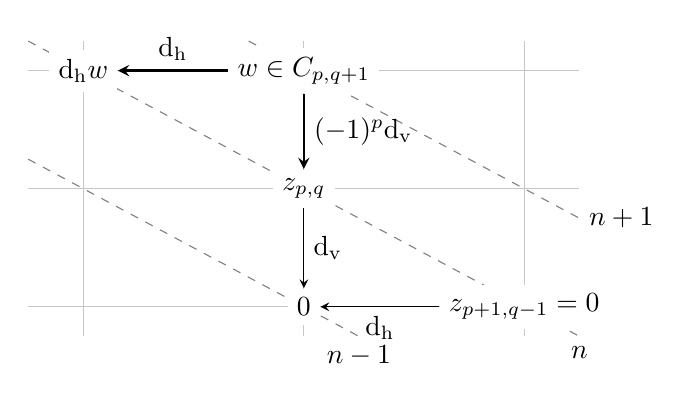
\begin{tikzpicture}[x=2.8cm,y=1.5cm,>=stealth]
\draw[gray!45,step=1] (-1.25,-1.25) grid (1.25,1.25);
\draw[dashed,gray] (-1.25,0.25)--(0.25,-1.25);
\draw[dashed,gray] (-1.25,1.25)--(1.25,-1.25);
\draw[dashed,gray] (-0.25,1.25)--(1.25,-0.25);
\node[fill=white] (w) at (0,1) {\(w\in C_{p,q+1}\)};
\node[fill=white] (z) at (0,0) {\(z_{p,q}\)};
\node[fill=white] (h) at (-1,1) {\(\mathrm d_{\mathrm h}w\)};
\node[fill=white] (v) at (0,-1) {\(0\)};
\node[fill=white] (r) at (1,-1) {\(z_{p+1,q-1}=0\)};
\draw[->,thick] (w)--(z) node[midway,right] {\((-1)^p\mathrm d_{\mathrm v}\)};
\draw[->,thick] (w)--(h) node[midway,above] {\(\mathrm d_{\mathrm h}\)};
\draw[->] (z)--(v) node[midway,right] {\(\mathrm d_{\mathrm v}\)};
\draw[->] (r)--(v) node[midway,below] {\(\mathrm d_{\mathrm h}\)};
\node[below] at (0.25,-1.25) {\(n-1\)};
\node[below] at (1.25,-1.25) {\(n\)};
\node[right] at (1.25,-0.25) {\(n+1\)};
\end{tikzpicture}
\end{center}
图中右侧分量为零，表示刚才选取最大横指标所排除的贡献。减去 \(\mathrm dw\) 消去 \(z_{p,q}\)，只在 \(C_{p-1,q+1}\) 留下修正 \(-\mathrm d_{\mathrm h}w\)，不会产生更右的分量。

于是 \(z-\mathrm{d}w\) 仍为圈，横指标 \(p\) 的分量已经消失，而新产生的分量至多位于横指标 \(p-1\)。第一象限中横指标不小于零，且次数 \(n\) 上只有 \(0\le p\le n\) 的位置；不断降低最大横指标，有限步后得到零。因此原圈是这些 \(w\) 的和的边界。横行正合时，交换两个指标；在 \(C_{p,q}\) 上乘符号 \((-1)^{pq}\)，给出交换前后两个全复形的同构，于是归入刚才的情形。
\end{proof}

\begin{lemma}[Tor 的平衡计算]\label{b3:lem:tor-balanced-computation}
设 \(R\) 为交换环，\(P_\bullet\rightarrow N\rightarrow0\) 与 \(Q_\bullet\rightarrow M\rightarrow0\) 为 \(R\) 模的自由消解。对每个整数 \(i\ge0\)，两条增广映射诱导自然同构
\[
H_i(P\otimes_RM)
\xleftarrow{\ \sim\ }H_i(\operatorname{Tot}(P\otimes_RQ))
\xrightarrow{\ \sim\ }H_i(N\otimes_RQ).
\]
因而用任一变量的自由消解都可计算 Tor，并有自然同构
\[
\operatorname{Tor}_i^R(N,M)\cong\operatorname{Tor}_i^R(M,N).
\]
\end{lemma}
\begin{proof}
取 \(C_{p,q}=P_p\otimes_RQ_q\)，水平、竖直微分分别为 \(\mathrm{d}_P\otimes1\)、\(1\otimes\mathrm{d}_Q\)。在纯张量上，全微分为
\[
\mathrm{d}(u\otimes v)=\mathrm{d}_Pu\otimes v+(-1)^p u\otimes\mathrm{d}_Qv.
\]
由 \(Q_0\twoheadrightarrow M\) 得到逐项满射
\(\alpha:\operatorname{Tot}(C)\rightarrow P\otimes_RM\)：它在 \(q=0\) 的分量上为增广映射，在 \(q>0\) 的分量上为零。这个映射把每条竖直消解在底端压到 \(P_p\otimes_RM\)。要保留被它删去的部分，核在 \(q>0\) 的位置仍取全部分量，底行则必须换成增广映射的核，而不能仍取整个 \(P_p\otimes_RQ_0\)。因此核是下面双复形 \(D\) 的全复形：
\[
D_{p,q}=P_p\otimes_RQ_q\quad(q>0),
\qquad
D_{p,0}=\ker(P_p\otimes_RQ_0\longrightarrow P_p\otimes_RM).
\]
水平微分与增广映射交换，所以保持底行的核；竖直微分从 \(q=1\) 出发时也落入这个核，故 \(D\) 确实是双复形。因为 \(P_p\) 自由，\(Q\) 的增广正合列张量 \(P_p\) 后仍正合，特别地从 \(P_p\otimes_RQ_1\) 到该底行核的映射满射。因此 \(D\) 的每条竖列正合，\cref{b3:lem:first-quadrant-column-exact}说明 \(\ker\alpha=\operatorname{Tot}(D)\) 正合。

这使 \(\alpha\) 在同调上成为同构：给 \(P\otimes_RM\) 中的圈任取提升，其微分落在核中；利用核的正合性减去适当核元素，便得到圈的提升。若全复形中的圈映为边界，先提升产生该边界的元素并减去它的微分，余下的圈落在核中，又是核中的边界。这分别证明满射与单射。

用 \(P_0\twoheadrightarrow N\) 得到另一条逐项满射
\(\beta:\operatorname{Tot}(C)\rightarrow N\otimes_RQ\)。此时将最左列 \(P_0\otimes_RQ_q\) 换成它到 \(N\otimes_RQ_q\) 的核，正是同样的截取。因每个 \(Q_q\) 自由，其核的每条横行正合，同一引理证明 \(\beta\) 也诱导同调同构。这就得到平衡计算。交换张量因子的映射
\[
u\otimes v\longmapsto(-1)^{pq}v\otimes u
\qquad(u\in P_p,\ v\in Q_q)
\]
保持全微分，并交换两条增广映射；于是得到 Tor 的对称性。对 \(N,M\) 的同态选比较链映射后，这些张量映射与增广映射交换；结合\cref{b3:cor:tor-well-defined-functor}的选择无关性，所述同构对两个变量都是自然的。因此以后选取较易消解的变量，并不会改变 Tor 模及其上由同态诱导的映射。
\end{proof}

\subsection{长正合列与 Koszul 计算}
\label{b3:subsec:1505:04}

\begin{lemma}\label{b3:lem:tor-basic-properties}
设 \(R\) 为交换环，\(N,M\) 为 \(R\) 模。Tor 具有自然同构
\[
\operatorname{Tor}_i^R(N,M)\cong\operatorname{Tor}_i^R(M,N)
\qquad(i\ge0),
\]
并在任一变量的短正合列上给出自然长正合列。例如，对 \(R\) 模短正合列
\(0\rightarrow M'\rightarrow M\rightarrow M''\rightarrow0\)，对整数 \(i\ge1\) 有
\[
\begin{aligned}
\cdots&\longrightarrow\operatorname{Tor}_i^R(N,M')
\longrightarrow\operatorname{Tor}_i^R(N,M)
\longrightarrow\operatorname{Tor}_i^R(N,M'')\\
&\xrightarrow{\delta}\operatorname{Tor}_{i-1}^R(N,M')
\longrightarrow\cdots\longrightarrow\operatorname{Tor}_1^R(N,M'')\\
&\xrightarrow{\delta}N\otimes_RM'
\longrightarrow N\otimes_RM
\longrightarrow N\otimes_RM''\longrightarrow0.
\end{aligned}
\]
若 \(a\in R\) 满足 \(aN=0\) 或 \(aM=0\)，则 \(a\operatorname{Tor}_i^R(N,M)=0\) 对每个 \(i\ge0\) 成立。若其中一个模平坦，则所有 \(i>0\) 的 Tor 为零。

对固定的 \(R\) 模 \(M\)，还有等价关系
\[
\begin{aligned}
M\;\text{平坦}
&\iff \operatorname{Tor}_1^R(N,M)=0
   \quad\text{对每个}\;R\;\text{模}\;N\\
&\iff \operatorname{Tor}_1^R(R/I,M)=0
   \quad\text{对每个理想}\;I\subseteq R.
\end{aligned}
\]
对任意理想 \(I,J\subseteq R\)，有自然同构
\[
\operatorname{Tor}_1^R(R/I,R/J)\cong(I\cap J)/IJ.
\]
\end{lemma}
\begin{proof}
对称性已由\cref{b3:lem:tor-balanced-computation}证明。固定 \(N\) 的自由消解 \(P\)，其各项自由，故给定短正合列张量 \(P_i\) 后仍正合，得到复形的逐项短正合列
\[
0\longrightarrow C'\xrightarrow{j}C\xrightarrow{q}C''\longrightarrow0,
\qquad
C'=P\otimes_RM',\quad C=P\otimes_RM,\quad C''=P\otimes_RM''.
\]
商复形中的圈任取一个提升后未必还是圈，但其微分误差必落在子复形中，并给出低一阶的圈；连接映射记录的就是这个误差的同调类。具体地，对 \(C''_i\) 中的圈 \(z''\)，取 \(C_i\) 中的提升 \(z\)。因 \(q(\mathrm{d}z)=0\)，存在唯一 \(z'\in C'_{i-1}\) 使 \(jz'=\mathrm{d}z\)。又由 \(j\) 单射及 \(j\mathrm{d}z'=\mathrm{d}^2z=0\)，有 \(\mathrm{d}z'=0\)。规定 \(\delta[z'']=[z']\)。改变提升只使 \(z'\) 增加一个边界；若 \(z''\) 增加边界 \(\mathrm{d}w''\)，提升 \(w''\) 并将其微分加到 \(z\) 上，\(z'\) 不变。因此连接映射良定义。

正合性在三类位置上直接核验。若 \(C\) 中的圈投到 \(C''\) 的边界，提升产生该边界的元素并减去其微分，便得到来自 \(C'\) 的圈。若 \(\delta[z'']=0\)，写 \(z'=\mathrm{d}v'\)，则 \(z-jv'\) 是 \(z''\) 的圈提升。若 \(C'\) 中的圈 \(z'\) 在 \(C\) 中成为边界 \(jz'=\mathrm{d}w\)，则 \(qw\) 为圈，且 \(\delta[qw]=[z']\)。这证明长列中各处正合；次数零的识别由\cref{b3:cor:tor-well-defined-functor}给出，末尾的满射由张量积右正合性得到。特别地，最低一段中 \(\delta\) 的像正是 \(N\otimes_RM'\to N\otimes_RM\) 的核，补回了张量后可能失去的单射信息。圈提升的构造与复形映射相容，故长列自然。第一变量的短正合列由平衡性得到相同结论。

若 \(aN=0\)，则 \(P\) 上的乘法 \(a\) 与零链映射都提升 \(N\) 上的零同态。\cref{b3:lem:free-resolution-comparison}给出它们之间的链同伦，张量 \(M\) 后仍成立，所以乘法 \(a\) 在同调上为零。若 \(aM=0\)，乘法 \(a\) 在 \(P\otimes_RM\) 上已为零。

若 \(M\) 平坦，令 \(Z_{-1}=N\)、\(Z_i=\ker\mathrm{d}_i\) 对 \(i\ge1\)，并令 \(Z_0=\ker(P_0\rightarrow N)\)。自由消解的正合性给出
\[
0\longrightarrow Z_i\longrightarrow P_i\longrightarrow Z_{i-1}\longrightarrow0
\qquad(i\ge0).
\]
每条短列张量 \(M\) 后仍正合，所以 \(P\otimes_RM\) 的正次数同调为零。若 \(N\) 平坦，交换两个变量即可。

反过来，若 \(\operatorname{Tor}_1^R(N,M)=0\) 对每个 \(N\) 成立，对任意短正合列 \(0\to U\to V\to W\to0\) 在第一变量中使用刚证的长列。\(\operatorname{Tor}_1^R(W,M)=0\) 使 \(U\otimes_RM\to V\otimes_RM\) 的核为零，故 \(M\) 平坦。更少的测试对象已经足够：对任意理想 \(I\)，因 \(R\) 自由，由 \(0\to I\to R\to R/I\to0\) 得到
\[
0\longrightarrow\operatorname{Tor}_1^R(R/I,M)
\longrightarrow I\otimes_RM\longrightarrow M.
\]
这里最后一个映射是 \(a\otimes m\mapsto am\)，所以 \(\operatorname{Tor}_1^R(R/I,M)\) 自然识别为理想张量判据中的核。若这些 Tor 对所有 \(I\) 都为零，\cref{b3:thm:ideal-flatness-criterion}便给出平坦性；前面已经证明平坦性使全部正次 Tor 消失，这完成所述等价关系。

在同一短列中取 \(M=R/J\)。映射
\(I\otimes_R(R/J)\to I/JI\)、\(a\otimes\bar r\mapsto ra+JI\)，与 \(a+JI\mapsto a\otimes\bar1\) 互逆；后一个映射良定义，因为 \(j\in J\) 时有 \(ja\otimes\bar1=a\otimes\bar j=0\)。因而得到
\[
0\longrightarrow\operatorname{Tor}_1^R(R/I,R/J)
\longrightarrow I/JI\longrightarrow R/J,
\qquad a+JI\longmapsto a+J.
\]
最后一个映射的核由恰好属于 \(J\) 的 \(a\in I\) 给出，即 \((I\cap J)/IJ\)。这证明交理想公式，且所有映射都来自包含、取商和张量积，因而同构自然。交 \(I\cap J\) 中未被乘积 \(IJ\) 消去的部分，由此成为一次 Tor 的具体表达。
\end{proof}

一般定义中的自由消解可以任意选择；当给定序列在 \(R\) 上正则时，前面构造的 Koszul 复形已经是 \(R/I\) 的自由消解，所以抽象的 Tor 可以直接用它的微分计算。

\begin{corollary}\label{b3:cor:koszul-tor}
设 \(R\) 为交换环，\(r\ge0\) 为整数，\(x=(x_1,\ldots,x_r)\) 是 \(R\) 上的正则序列，\(I=(x_1,\ldots,x_r)\)。对任意 \(R\) 模 \(M\) 与整数 \(i\ge0\)，有
\[
\operatorname{Tor}_i^R(R/I,M)\cong H_i(x;M).
\]
若 \(IM=0\)，则 \(\operatorname{Tor}_i^R(R/I,M)\cong M^{\binom ri}\) 对 \(0\le i\le r\) 成立，\(i>r\) 时为零。

特别地，设 \(k\) 为域，\(d\ge0\) 为整数，令
\[
R=k[X_1,\ldots,X_d]_{(X_1,\ldots,X_d)},
\qquad \mathfrak m=(X_1,\ldots,X_d)R,
\]
其剩余域 \(R/\mathfrak m\) 自然识别为 \(k\)。则对 \(0\le i\le d\)，有
\[
\operatorname{Tor}_i^R(k,k)\cong\bigwedge_k^ik^d,
\qquad
\dim_k\operatorname{Tor}_i^R(k,k)=\binom di;
\]
对 \(i>d\)，有 \(\operatorname{Tor}_i^R(k,k)=0\)。
\end{corollary}
\begin{proof}
用\cref{b3:thm:koszul-regular-resolution}给出的自由消解计算 Tor。若 \(IM=0\)，张量后的每个微分项 \(x_jm\) 都为零，同调就是复形本身各项，即所述的有限直和。

在局部多项式模型中，模掉 \(X_1,\ldots,X_{j-1}\) 后得到整环
\(k[X_j,\ldots,X_d]_{(X_j,\ldots,X_d)}\)，其中 \(X_j\) 非零，所以乘 \(X_j\) 单射。最终商为非零域 \(k\)，故变量序列是 \(R\) 正则序列；\(d=0\) 时则是空序列。其 Koszul 自由消解张量 \(k\) 后，所有 \(X_j\) 都作用为零，于是微分全为零，第 \(i\) 项按递增指标楔积基识别为 \(\bigwedge_k^ik^d\)。这组基的数目为 \(\binom di\)，且次数超过 \(d\) 时复形本身已经为零，得到所述同调与维数。
\end{proof}

在这个局部多项式模型中，\(k^d\) 通过标准基送到 \(X_j+\mathfrak m^2\)，识别为余切空间 \(\mathfrak m/\mathfrak m^2\)。因此一次 Tor 保留这些一次函数类，高次 Tor 则给出它们的外幂；由\cref{b3:prop:tangent-cotangent-rational}，切空间是这个余切空间的 \(k\) 线性对偶。


\begin{chaptersummary}
正则序列的条件施加在逐次商上，不能只在原环中检验各元素。局部环上的有限生成模中，Nakayama 引理保证商不消失，Krull 交定理则使相邻元素可以交换次序。

\ProseParagraphBreak
Koszul 微分由删去外积因子和交替符号构成；微分平方为零来自同一对因子的两种删法相消。加进一个元素，相当于把原复形与其移位组合起来，其连接映射就是该元素的乘法。这条正合列既证明正则序列给出消解，也把局部逆命题归结为有限生成同调模上的 Nakayama 引理。

\ProseParagraphBreak
自由消解张量后出现的同调是 Tor。消解之间的比较映射在链同伦意义下唯一，因而这些同调不依赖消解的选择，并具有两变量的函子性。一个正则序列的 Koszul 消解在被该序列零化的模上变成零微分复形，因而能直接计算 Tor；商环有多个不可约分量或非零幂零元，并不自动破坏原序列的正则性。
\end{chaptersummary}

\BookExercises

\begin{exercise}\label{b3:ex:15-module-choice}
设 \(k\) 为域，\(R=k[X,Y]\)。分别判断 \(X\) 在 \(R/(Y)\)、\(R/(X)\)、\(R/(XY)\) 上是否为非零因子；在成立时，判断单元素序列 \(X\) 是否正则。
\end{exercise}
\begin{solution}
第一模同构于 \(k[X]\)，乘 \(X\) 单射且商为 \(k\)，故序列正则。第二模中 \(X\) 作用为零而模非零，故不是非零因子。第三模中非零的 \(\bar Y\) 被 \(X\) 零化，也不成立。
\end{solution}

\begin{exercise}\label{b3:ex:15-powers}
设 \(R\) 为交换环，\(M\ne0\) 为 \(R\) 模，\(x,y\) 是 \(M\) 正则序列。证明对任意正整数 \(a,b\)，\(x^a,y^b\) 仍为 \(M\) 正则序列。
\end{exercise}
\begin{solution}
\(x^a\) 显然单射。证明 \(y\) 在 \(M/x^aM\) 上单射：若 \(ym=x^an\)，模掉 \(xM\) 得 \(m=xm_1\)，约去 \(x\) 后有 \(ym_1=x^{a-1}n\)，反复进行得 \(m\in x^aM\)。所以 \(y^b\) 也在该商上单射。末端商 \(M/(x^a,y^b)M\) 满射到非零的 \(M/(x,y)M\)，因而非零。
\end{solution}

\begin{exercise}\label{b3:ex:15-order-localization}
设 \(k\) 为域，\(R=k[X,Y]\)，\(M=R\oplus R/(X-1,Y)\)。在极大理想 \((X,Y)\) 处局部化，解释为何原来不正则的次序 \(Y,X\) 在 \(M_{(X,Y)}\) 上变成正则。
\end{exercise}
\begin{solution}
\(X-1\) 在该局部环中是单位，故第二直和项局部化为零，剩下 \(k[X,Y]_{(X,Y)}\)。先模掉 \(Y\) 得 \(k[X]_{(X)}\)，其中 \(X\) 为非零因子，末端商为 \(k\)，所以 \(Y,X\) 正则。原来的乘法核全部位于被这次局部化删去的支集部分。
\end{solution}

\begin{exercise}\label{b3:ex:15-flat-not-faithful}
设 \(k\) 为域，取 \(R=k[T]\times k[T]\)，\(S=k[T]\) 为投影到第一因子的 \(R\) 代数，\(x=(T,0)\)。证明 \(S\) 平坦但不忠实，并说明 \(x\) 在 \(S\) 上正则不能推出它在 \(R\) 上正则。
\end{exercise}
\begin{solution}
\(S\) 作为 \(R\) 模是幂等元 \((1,0)\) 给出的直和项，故投射、从而平坦。非零模 \(0\times k[T]\) 与 \(S\) 张量为零，所以不忠实。\(x\) 在 \(S\) 上就是 \(T\)，乘法单射且商为 \(k\)；在 \(R\) 上却零化非零元 \((0,1)\)。
\end{solution}

\begin{exercise}\label{b3:ex:15-koszul-localize-unit}
设 \(k\) 为域，\(R=k[X,Y]\)，\(M=R_X\oplus R_Y\)。计算 \(H_i(X,Y;M)\)，并证明虽然 \(I=(X,Y)\) 是 \(R\) 的真理想，却有 \(IM=M\)。判断该序列是否 \(M\) 正则，并说明 \(M_{(X,Y)}\) 是否为非零有限生成模。
\end{exercise}
\begin{solution}
复形按两个系数模分成直和。在 \(R_X\) 上用 \(X^{-1}e_1\wedge(-)\)，在 \(R_Y\) 上用 \(Y^{-1}e_2\wedge(-)\)，所得同伦均满足 \(\mathrm{d}h+h\mathrm{d}=\operatorname{id}\)，所以全部同调为零。又因 \(XR_X=R_X\)、\(YR_Y=R_Y\)，有 \(IM=M\)。末端商为零，序列不满足本章正则序列的非退化条件。

\ProseParagraphBreak
在 \(\mathfrak m=(X,Y)\) 处，\(M_{\mathfrak m}=R_{\mathfrak m}[X^{-1}]\oplus R_{\mathfrak m}[Y^{-1}]\) 非零，因为这两个局部化都嵌入 \(R\) 的分式域。若它有限生成，由 \(\mathfrak mM_{\mathfrak m}=M_{\mathfrak m}\) 和 Nakayama 引理便得 \(M_{\mathfrak m}=0\)，矛盾。因此它不是有限生成模，不能套用局部有限生成模的 Koszul 正则性判据。
\end{solution}

\begin{exercise}\label{b3:ex:15-three-matrices}
对任意交换环 \(R\) 中的 \(x,y,z\)，在二次外幂中采用基 \(e_1\wedge e_2,e_1\wedge e_3,e_2\wedge e_3\)，写出 \(K_\bullet(x,y,z;R)\) 的三个微分矩阵，并计算相邻矩阵乘积。
\end{exercise}
\begin{solution}
三个矩阵依次为
\[
\mathrm{d}_1=(x\ \ y\ \ z),\qquad
\mathrm{d}_2=\begin{pmatrix}-y&-z&0\\x&0&-z\\0&x&y\end{pmatrix},
\qquad \mathrm{d}_3=\begin{pmatrix}z\\-y\\x\end{pmatrix}.
\]
\(\mathrm{d}_1\mathrm{d}_2\) 的分量为 \(-xy+yx,-xz+zx,-yz+zy\)，均为零；\(\mathrm{d}_2\mathrm{d}_3\) 的分量为 \(-yz+zy,xz-zx,-xy+yx\)，也均为零。这里只用交换性，特征二时两项仍相消。
\end{solution}

\begin{exercise}\label{b3:ex:15-generator-operation}
设 \(R\) 为交换环，\(x,y,a\in R\)，\(M\ne0\) 为 \(R\) 模。构造 \(K_\bullet(x,y+ax;R)\) 与 \(K_\bullet(x,y;R)\) 的同构，并说明替换 \(y\) 为 \(y+ax\) 是否改变 \(x,y\) 在 \(M\) 上的正则性。
\end{exercise}
\begin{solution}
把新一次基 \(f_1,f_2\) 分别送到 \(e_1,e_2+ae_1\)。其微分分别为 \(x,y+ax\)，且基变换矩阵行列式为一，故在全部外幂上给出可逆链映射。张量 \(M\) 后仍为同构。正则性可直接由定义判断：第一步仍是乘 \(x\)，而在 \(M/xM\) 上有
\[
(y+ax)m\equiv ym\pmod{xM},
\qquad (x,y+ax)M=(x,y)M.
\]
因此第二步的乘法映射及末端商都没有改变，\(x,y\) 与 \(x,y+ax\) 的正则性等价。
\end{solution}

\begin{exercise}\label{b3:ex:15-repeated-equation}
设 \(R\) 为整环，\(0\ne x\in R\) 为非单位元。计算 \(K_\bullet(x,x,x;R)\) 的全部同调，并写出次数一、二同调的生成圈。
\end{exercise}
\begin{solution}
换基为 \(g_1=e_1\)、\(g_2=e_2-e_1\)、\(g_3=e_3-e_1\)。这是行列式为一的整数换基，且 \(\mathrm{d}g_1=x\)、\(\mathrm{d}g_2=\mathrm{d}g_3=0\)。因此复形分成四个由 \(1,g_2,g_3,g_2\wedge g_3\) 标记的两项复形，微分在每个非零配对中都是乘 \(x\)（至多相差符号）。乘 \(x\) 单射，故
\[
H_0=R/(x),\qquad H_1=(R/(x))^2,\qquad H_2=R/(x),\qquad H_3=0.
\]
次数一的两组生成圈为 \(g_2,g_3\)，次数二的生成圈为 \(g_2\wedge g_3\)。这些类的系数均模掉 \((x)\)；三次同调为零来自乘 \(x\) 的单射性。
\end{solution}

\begin{exercise}\label{b3:ex:15-dual-numbers}
设 \(k\) 为域，令 \(R=k[\varepsilon]/(\varepsilon^2)\)。分别计算 \(K_\bullet(\varepsilon;R)\) 与 \(K_\bullet(\varepsilon;R/(\varepsilon))\) 的同调，并比较原因。
\end{exercise}
\begin{solution}
第一复形中乘法核为 \((\varepsilon)\cong k\)，余核也为 \(k\)。第二复形的微分为零，所以两处同调都为 \(k\)。前者的非正合性来自环中真实的零因子，后者则因为张量系数模使乘法完全消失。
\end{solution}

\begin{exercise}\label{b3:ex:15-crossing-homology}
设 \(k\) 为域，\(R=k[X,Y]/(XY)\)，\(\bar X,\bar Y\) 为变量的余类。计算 \(H_i(\bar X,\bar Y;R)\)。
\end{exercise}
\begin{solution}
把 \(R\) 写成常数项相同的多项式配对，可知 \(\operatorname{Ann}(\bar X)=(\bar Y)\)、\(\operatorname{Ann}(\bar Y)=(\bar X)\)，两理想交为零。一次圈恰为 \((\bar Ya,\bar Xb)\)，边界为 \((-\bar Yc,\bar Xc)\)。取 \(c=1\) 得
\[
[(0,\bar X)]=[(\bar Y,0)]\quad\text{于 }H_1.
\]
这一类被 \(\bar X,\bar Y\) 零化：乘 \(\bar X\) 直接得零，乘 \(\bar Y\) 则得到边界 \((\bar Y^2,0)=\mathrm{d}_2(-\bar Y)\)。同样，\(\bar Y,\bar X\) 的二次及更高次幂给出的圈都是边界，所以任意圈都化成该类的 \(k\) 倍。这个类非零，否则须有 \(c\) 同时满足 \(-\bar Yc=\bar Y\)、\(\bar Xc=0\)，前式要求其常数项为 \(-1\)，后式要求为零，矛盾。因此 \(H_1\cong k\)，最高同调为上述零化子之交，故 \(H_2=0\)，而 \(H_0=k\)。
\end{solution}

\begin{exercise}\label{b3:ex:15-triangular-complete-intersection}
设 \(k\) 为域，\(R=k[X,Y,Z]\)。证明 \(Y-X^2,Z-Y^2,Z\) 是正则序列，计算末端商的 \(k\) 维数，并写出自由消解各项的秩。
\end{exercise}
\begin{solution}
依次前两次商为 \(k[X,Z]\)、\(k[X]\)，所以前两步乘法都是整环中非零元的乘法。此时 \(Z\) 的像为 \(X^4\)，仍为非零因子，末端商为 \(k[X]/(X^4)\)，维数为四。三元 Koszul 消解从次数零至三的秩依次为 \(1,3,3,1\)。
\end{solution}

\begin{exercise}\label{b3:ex:15-component-section}
设 \(k\) 为域，令 \(A=k[U,V]/(UV)\)，仍以 \(U,V\) 记变量的余类。对 \(a,b\in k\)，判断 \(aU+bV\) 何时在 \(A\) 上为非零因子，并在成立时求其商环。
\end{exercise}
\begin{solution}
若 \(a=0\)，则该元素被非零的 \(U\) 零化；\(b=0\) 同理。若 \(a,b\ne0\)，用常数项相同的配对模型，乘法分别为乘 \(aU,bV\)，故单射。在商中 \(V=-ab^{-1}U\)，关系 \(UV=0\) 变成 \(U^2=0\)，所以商环为 \(k[U]/(U^2)\)。
\end{solution}

\begin{exercise}\label{b3:ex:15-tor-integers}
设 \(m,n\) 为正整数，计算 \(\operatorname{Tor}_i^{\mathbb Z}(\mathbb Z/m,\mathbb Z/n)\) 对所有 \(i\ge0\) 的值。
\end{exercise}
\begin{solution}
用 \(\mathbb Z\xrightarrow{m}\mathbb Z\) 的自由消解。张量后为 \(\mathbb Z/n\xrightarrow{m}\mathbb Z/n\)。若 \(d=\gcd(m,n)\)，其核由 \(n/d\) 的余类生成，阶为 \(d\)，余核也为 \(\mathbb Z/d\)。因此次数零、一均为 \(\mathbb Z/d\)，其余次数为零。
\end{solution}

\begin{exercise}\label{b3:ex:15-intersection-tor}
设 \(k\) 为域，\(R=k[X,Y,Z]\)，\(I=(X,Y)\)、\(J=(Y,Z)\)。计算 \(\operatorname{Tor}_i^R(R/I,R/J)\) 对所有 \(i\ge0\) 的值；再计算 \((I\cap J)/IJ\)，与次数一的答案比较。
\end{exercise}
\begin{solution}
\(X,Y\) 正则，其 Koszul 消解张量 \(R/J=k[X]\) 后成为 \(K_\bullet(X,0;k[X])\)。乘 \(X\) 单射，因此次数零、一同调均为 \(k\)，其余同调为零。

\ProseParagraphBreak
模掉 \(Y\) 后，\(k[X,Z]\) 中 \((X)\cap(Z)=(XZ)\)，故
\[
I\cap J=(Y,XZ),\qquad IJ=(XY,XZ,Y^2,YZ).
\]
商由 \(Y\) 的类生成；它被 \(X,Y,Z\) 零化而不为零，因为 \(Y\notin IJ\)。这个商因而同构于 \(k\)，与正文的交理想公式及上述 \(\operatorname{Tor}_1\) 计算一致。
\end{solution}

\begin{exercise}\label{b3:ex:15-residue-tor}
设 \(k\) 为域，\(R=k[X,Y]_{(X,Y)}\)，\(a,b\ge2\) 为整数，\(A=R/(X^a,Y^b)\)。计算 \(\operatorname{Tor}_i^R(k,A)\)，并在 \(K_\bullet(X,Y;A)\) 中写出同调的 \(k\) 基。
\end{exercise}
\begin{solution}
\(X^a,Y^b\) 在多项式环中正则，局部化后末端商仍非零，故也是 \(R\) 正则序列。其 Koszul 消解张量 \(k\) 后微分为零，得到 \(\operatorname{Tor}_i^R(A,k)\) 在次数零、一、二的维数分别为 \(1,2,1\)，其余为零。由平衡性，\(\operatorname{Tor}_i^R(k,A)\) 同样如此。

\ProseParagraphBreak
\(A\) 同构于 \(k[X,Y]/(X^a,Y^b)\)：在后一个环中，常数项非零的元素都是单位，因为其余部分幂零。它有基 \(X^iY^j\)（\(0\le i<a,0\le j<b\)）。在 \(K_\bullet(X,Y;A)\) 中，\(H_0\) 的基为 \([1]\)，\(H_1\) 的候选基为
\[
[X^{a-1}e_1],\qquad [Y^{b-1}e_2],
\]
\(H_2\) 的候选基为 \([X^{a-1}Y^{b-1}e_1\wedge e_2]\)。它们都是圈。若一次圈的上述 \(k\) 线性组合是边界 \((-Yc,Xc)\)，第一分量模掉 \(Y\)、第二分量模掉 \(X\)，分别迫使两个系数为零，所以两类独立。次数二的圈非零且无三次边界。结合已算出的同调维数，这些类分别构成所需的基。
\end{solution}

\begin{exercise}\label{b3:ex:15-zero-generator-splitting}
设 \(R\) 为交换环，\(M\) 为 \(R\) 模，\(r\ge0\) 为整数，\(x=(x_1,\ldots,x_r)\in R^r\)。证明
\[
H_i(x,0;M)\cong H_i(x;M)\oplus H_{i-1}(x;M),
\]
并由此计算 \(r\) 个零元素在 \(M\) 上的 Koszul 同调。
\end{exercise}
\begin{solution}
新增元素为零时，分解 \(K_i(x,0;M)=K_i(x;M)\oplus K_{i-1}(x;M)\) 的微分是 \((a,b)\mapsto(\mathrm{d}a,-\mathrm{d}b)\)，两个分量不混合，故同调分裂如式。从空序列的唯一同调 \(M\) 开始反复应用，得到 \(H_i(0,\ldots,0;M)\cong M^{\binom ri}\)，超出 \(0\le i\le r\) 的次数为零。
\end{solution}

\begin{exercise}\label{b3:ex:15-infinite-module-caution}
设 \(R\) 为离散赋值环，统一化元为 \(\pi\)，分式域为 \(K\)。计算 \(K_\bullet(\pi;K)\) 的同调，说明为何不能由次数一同调为零断言 \(\pi\) 是本章意义的 \(K\) 正则序列。
\end{exercise}
\begin{solution}
\(\pi:K\rightarrow K\) 是同构，所以两处同调都为零。末端商 \(K/\pi K=0\)，违反非退化条件。\(K\) 不是有限生成的 \(R\) 模，Nakayama 引理不能用于证明末端商非零，所以局部环上有限生成模的判据不适用。
\end{solution}

\begin{exercise}\label{b3:ex:15-local-detection-obstruction}
设 \(k\) 为域，\(R=k[X,Y,Z]\)。对序列 \(XY,XZ\)，求正次数 Koszul 同调的支集，与 \(V(XY,XZ)\) 比较，并分别判断在素理想 \((X)\)、\((Y,Z)\)、\((Y)\) 处的同调及正则性。
\end{exercise}
\begin{solution}
一次圈满足 \(XYa+XZb=0\)，约去 \(X\) 后得 \(Ya+Zb=0\)，故恰为 \((-Zc,Yc)\)。一次边界为 \(X(-Zc,Yc)\)，而最高微分单射，所以
\[
H_1\cong R/(X),\qquad H_2=0,\qquad
\operatorname{Supp}H_1=V(X)\subsetneq V(X)\cup V(Y,Z)=V(XY,XZ).
\]
在 \((X)\) 处，\(Y,Z\) 都成为单位，两个方程都是 \(X\) 的单位倍，末端商非零且 \(H_1\ne0\)，第二个方程重复了第一个，序列不正则。在 \((Y,Z)\) 处，\(X\) 是单位，序列的正则性等同于 \(Y,Z\) 的正则性；逐次商为整环，末端商是 \(k(X)\)，故序列正则且正次数同调全为零。在 \((Y)\) 处，\(XZ\) 是单位，全部同调与末端商都为零，所以仍不符合本章非退化意义的正则性。
\end{solution}

% !TeX root = ../../Book3.tex
% 纲要标题：## 第16章　深度与 Serre 条件
% 纲要位置：工作记录/计划纲要.md，第 2485 行。
% 纲要细目（写作范围）：

\chapter{深度与 Serre 条件}
\label{b3:ch:16}
\BookChapterNumber{b3:ch:16}

\begin{chapterabstract}
深度把局部环上的有限生成模中能够依次选取的正则元素个数变成一个不依赖选择的整数。本章先用 Koszul 同调比较所有极大正则序列，再证明深度等于剩余域的 Ext 首次非零次数。借助这一刻画，建立短正合列中的深度引理、关联素理想的维数估计和局部化不等式，并把各点的深度要求整理为 Serre 条件。这些结果为投射维数、Cohen--Macaulay 模与局部上同调提供共同的计算依据。
\end{chapterabstract}

\begin{learninggoals}
\begin{itemize}
\item 证明极大正则序列同长度，区分“不能延长”与预先假定“长度最大”。
\item 说明有限性在深度零判据、Ext 模及局部化估计中的作用。
\item 用短正合列比较深度，并辨别何时只有下界、何时可以取得等式。
\item 在全部相关素理想处检查 \((S_k)\)，用关联素理想解释 \((S_1)\) 的含义。
\end{itemize}
\end{learninggoals}

设 \(k\) 为域。在局部环 \(R=k[x,y]_{(x,y)}/(xy)\) 中，以下用 \(x,y\) 表示它们的剩余类。\(x\) 和 \(y\) 都是零因子，但 \(x+y\) 不是：它在两个整环商 \(R/(x)\)、\(R/(y)\) 中的像都非零，而 \(R\) 嵌入这两个商的直和。因此仍可从极大理想中选出一个非零因子。若改为 \(k[x,y]_{(x,y)}/(x^2,xy)\)，非零的 \(\bar x\) 被极大理想的每个元素杀死，连第一步都无从开始。两个环的 Krull 维数都为一，正则元素可选取的长度却不同。维数测量素理想链的长度，深度则测量还能连续选取多少个非零因子；后一环的 \(y\) 方向仍然存在，但闭点处由 \(\bar x\) 生成的部分已阻止任何正则切割。

\ProseParagraphBreak

若只按某次选择数出正则元素，就要证明换一种选择不会改变所得最大长度。Koszul 同调与剩余域的 Ext 给出不依赖选择的检验方式；短正合列与局部化又让这种数值在模之间、在不同点之间比较。由此得到的深度不等式，将把可见的维数与隐藏的嵌入结构分开。

\ProseParagraphBreak

本章使用\chapref{b3:ch:15}的正则序列与 Koszul 同调，以及\chapref{b3:ch:04}的关联素理想、\chapref{b3:ch:09}的维数和参数系。\secref{b3:sec:1505}已证明自由消解的存在性，以及比较映射在同伦意义下的唯一性；\secref{b3:sec:1602}据此定义 Ext，建立双变量长正合列，并证明所需的有限性和局部化性质。第四卷第6—9章系统讨论这些同调函子的理论，\chapref{b3:ch:22}则用局部上同调给出深度的另一种刻画。

\ProseParagraphBreak
正则序列长度与 Ext、Koszul 同调之间的关系，可对照松村英之的《Commutative Ring Theory》\cite[\S16, Theorems 16.6--16.8, pp. 129--131]{Matsumura1989CommutativeRingTheory}。本章用于局部化估计的消失引理和关联素理想维数界，对应该书的 Theorems 17.1--17.2\cite[pp. 133--134]{Matsumura1989CommutativeRingTheory}；环的 Serre 条件在该书 \S23, p. 183 中集中说明\cite[\S23, p. 183]{Matsumura1989CommutativeRingTheory}。本章同时明确有限生成模版本所使用的支集维数。

% !TeX root = ../../Book3.tex
% 纲要标题：### 16.1 深度
% 纲要位置：工作记录/计划纲要.md，第 2487 行。
% 纲要细目（写作范围）：
% * 极大正则序列长度
% * 深度的有限性与存在性、基座及深度零与有限长度子模的判据
% * 深度不超过维数；非约化环的正深度

\section{深度}
\label{b3:sec:1601}

维数数的是素理想链，正则序列则问有多少个元素能够依次以单射作用。后一种长度似乎依赖选择：一个不能再延长的序列，是否可能比另一个短？局部有限性使这些长度相同，Koszul 同调给出一个可以同时比较所有选择的量，其共同长度就是深度。


% 纲要内容（仅作写作计划，尚非教材正文）：
%
% * 极大正则序列长度
% * 深度的有限性与存在性、基座及深度零判据
% * 深度不超过维数
%

\subsection{极大正则序列的长度}
\label{b3:subsec:1601:01}

\begin{definition}\label{b3:def:maximal-regular-sequence}
设 \((R,\mathfrak m)\) 为交换 Noether 局部环，\(M\ne0\) 为有限生成的 \(R\) 模。若 \(x_1,\ldots,x_t\in\mathfrak m\) 为 \(M\) 正则序列，而且不能再添上任何 \(y\in\mathfrak m\) 得到更长的正则序列，则称它为 \(\mathfrak m\) 中的一个\term[jida-zhengze-xulie]{极大正则序列}[maximal regular sequence]。这里“极大”指不能延长，尚未预先断言其长度最大。
\end{definition}

不能延长只说明当前选择已到尽头，一般并不能保证不同选择具有相同长度。下面用同一组极大理想生成元的 Koszul 同调比较这些选择，证明正则序列在这里确实有一个共同的最大长度。

\begin{theorem}\label{b3:thm:maximal-regular-length}
设 \((R,\mathfrak m)\) 为交换 Noether 局部环，\(M\ne0\) 为有限生成的 \(R\) 模。每个由 \(\mathfrak m\) 中元素构成的 \(M\) 正则序列都能延长为极大正则序列，且所有极大正则序列长度相同。若取 \(\mathfrak m=(y_1,\ldots,y_e)\) 的任意有限生成组，不必为极小生成组，其共同长度为
\[
e-\max\{\,i\mid H_i(y_1,\ldots,y_e;M)\ne0\,\}.
\]
\end{theorem}
\begin{proof}
每添加一个正则元素，已选元素生成的理想严格增大：若新元素在原理想中，它在非零的逐次商上作用为零，不可能单射。Noether 环的理想升链条件保证这个过程在有限步停止。

先看非零有限生成模 \(N\) 上的空序列何时已经极大。对 \(x\in\mathfrak m\)，Nakayama 引理保证 \(N/xN\ne0\)，所以能否添加 \(x\) 只取决于乘 \(x\) 是否单射。空序列极大便意味着 \(\mathfrak m\) 中每个元素都是 \(N\) 的零因子。由\cref{b3:thm:associated-zero-divisors}，
\[
\mathfrak m\subseteq\bigcup_{\mathfrak p\in\operatorname{Ass}_RN}\mathfrak p.
\]
因 \(R\) Noether 且 \(N\) 有限生成，\(\operatorname{Ass}_RN\) 是有限集，故\cref{b3:lem:finite-prime-avoidance}适用，给出 \(\mathfrak m\) 包含于某个 \(\mathfrak p\in\operatorname{Ass}_RN\)。局部环中每个素理想都包含于 \(\mathfrak m\)，于是 \(\mathfrak p=\mathfrak m\)。存在 \(n\ne0\) 满足 \(\mathfrak mn=0\)。因此 Koszul 最高同调
\[
H_e(y;N)=\{\,n\in N\mid\mathfrak mn=0\,\}
\]
非零，且没有次数超过 \(e\) 的项。反过来，这样的 \(n\) 也使 \(\mathfrak m\) 中任何元素都不可能正则。因此找不到第一个正则元素时，已有同一个非零元素被整个极大理想零化，而不是只有不同元素各自被某些零因子零化。

对任意非零有限生成模 \(N\)，令 \(q(N)=\max\{i\mid H_i(y;N)\ne0\}\)。这个最大值存在：由\cref{b3:thm:nakayama}，\(H_0=N/\mathfrak mN\ne0\)，而复形只有次数零到 \(e\) 的项。要比较取正则商前后的最高非零次数，关键是 \(x\in\mathfrak m=(y_1,\ldots,y_e)\)，所以\cref{b3:prop:koszul-signs-homotopy}给出 \(xH_i(y;N)=0\)。

若 \(x\in\mathfrak m\) 在 \(N\) 上正则，将短正合列 \(0\rightarrow N\xrightarrow{x}N\rightarrow N/xN\rightarrow0\) 张量 \(K_\bullet(y;R)\)。该复形的每一项都是有限秩自由模，故得到逐项短正合列。按\cref{b3:lem:tor-basic-properties}证明中的圈提升构造，它诱导同调长正合列。在 \(H_i(y;N/xN)\) 的两侧，长列的乘法 \(x\) 都为零，因此长列分成短正合列
\[
0\longrightarrow H_i(y;N)\longrightarrow H_i(y;N/xN)
\longrightarrow H_{i-1}(y;N)\longrightarrow0
\]
正合。令 \(q=q(N)\)，则 \(H_{q+1}(y;N)=0\)、\(H_q(y;N)\ne0\)。取 \(i=q+1\)，上列给出
\[
H_{q+1}(y;N/xN)\xrightarrow{\sim}H_q(y;N)\ne0.
\]
当 \(i>q+1\) 时，短正合列的两端均为零，中间项也为零。因此每除去一个正则元素，最高非零 Koszul 同调次数恰好上移一位，即 \(q(N/xN)=q(N)+1\)。若极大正则序列长为 \(t\)，它的非零末端商已找不到正则元素，前面的空序列判据说明该商的最高非零同调次数为 \(e\)。连续应用这个等式便得到 \(e=q(M)+t\)。右端除 \(t\) 外不依赖所选序列，故所有长度相同。
\end{proof}

这里的 \(e\) 是所选生成组的长度，不一定等于嵌入维数。例如，对域 \(k\)，在 \(R=k[X,Y]_{(X,Y)}\) 中，\(X,Y\) 是正则序列，所以 \(H_0(X,Y;R)=k\)，正次数同调为零，最高非零次数为 \(0\)。也可以用 \(X,Y,X\) 生成极大理想。把第三个元素减去第一个元素，由\cref{b3:prop:koszul-generator-change}将其复形换成 \(K_\bullet(X,Y,0;R)\)。张量分解中的 \(K_\bullet(0;R)\) 在次数零、一各有一个 \(R\)，微分为零，故
\[
H_i(X,Y,X;R)
\cong H_i(X,Y;R)\oplus H_{i-1}(X,Y;R).
\]
于是这一冗余生成组的零次和一次同调都是 \(k\)，更高同调为零；公式中的差由 \(2-0\) 变成 \(3-1\)，共同长度仍为 \(2\)。

\subsection{深度的存在性与有限性}
\label{b3:subsec:1601:02}

\begin{definition}\label{b3:def:depth}
设 \((R,\mathfrak m)\) 为交换 Noether 局部环，\(M\ne0\) 为有限生成的 \(R\) 模。\(\mathfrak m\) 中任一极大 \(M\) 正则序列的长度称为 \(M\) 在 \(R\) 上的\term[shendu]{深度}[depth]，记为 \(\operatorname{depth}_RM\)。约定 \(\operatorname{depth}_R0=+\infty\)；环的深度是其作为自身模的深度。
\end{definition}
\symidx{\(\operatorname{depth}_RM\)：局部模的深度}

定义的选择无关性由\cref{b3:thm:maximal-regular-length}保证，也说明非零有限生成模的深度是有限非负整数。固定极大理想的有限生成组后，它不超过生成元数。零模取无穷大的约定只用于公式，不把零模解释为可以在本章定义下具有任意长正则序列的对象。

\begin{corollary}\label{b3:cor:depth-zero-socle}
设 \((R,\mathfrak m)\) 为交换 Noether 局部环，\(k=R/\mathfrak m\) 为其剩余域，\(M\ne0\) 为有限生成的 \(R\) 模。以下条件等价：
\begin{equivalences}
\item \(\operatorname{depth}_RM=0\)；
\item \(\mathfrak m\in\operatorname{Ass}_RM\)；
\item \(\operatorname{Hom}_R(k,M)\ne0\)；
\item \(M\) 含有非零有限长度子模。
\end{equivalences}
\end{corollary}
\begin{proof}
前两个条件的等价已在\cref{b3:thm:maximal-regular-length}的证明中得到。一个同态 \(k\rightarrow M\) 由 \(1+\mathfrak m\) 的像决定，该像恰为被 \(\mathfrak m\) 零化的元素；非零时其零化子等于 \(\mathfrak m\)，故第二、第三个条件等价。这样的非零同态从简单模 \(k\) 出发，必为单射，其像是长度一的子模，因而得到第四个条件。

反过来，设 \(0\ne L\subseteq M\) 具有有限合成列 \(0=L_0\subsetneq L_1\subsetneq\cdots\subsetneq L_\ell=L\)。局部环上的每个简单商 \(L_j/L_{j-1}\) 都同构于 \(k\)，所以 \(\mathfrak mL_j\subseteq L_{j-1}\)。沿合成列逐步相乘得到 \(\mathfrak m^\ell L=0\)。取使 \(\mathfrak m^aL=0\) 的最小正整数 \(a\)，则 \(\mathfrak m^{a-1}L\ne0\)，其中的非零元素被 \(\mathfrak m\) 零化，于是给出非零同态 \(k\to M\)。这证明第四个条件蕴含第三个条件。
\end{proof}

这样的简单子模可能不唯一；把模中的所有简单子模合在一起，就得到下面的子模。

\begin{definition}\label{b3:def:socle}
设 \((R,\mathfrak m)\) 为交换局部环，\(k=R/\mathfrak m\) 为其剩余域，\(M\) 为 \(R\) 模。\(M\) 中全部简单子模之和称为 \(M\) 的\term[jizuo]{基座}[socle]，记为 \(\operatorname{Soc}_RM\)。在此局部环情形，有
\[
\operatorname{Soc}_RM=(0:_M\mathfrak m)
=\{\,u\in M\mid au=0\text{ 对所有 }a\in\mathfrak m\,\}.
\]
\end{definition}
\symidx{\(\operatorname{Soc}_RM\)：模的基座}

每个简单 \(R\) 模都同构于 \(k\)，因此被 \(\mathfrak m\) 零化；反过来，若 \(u\ne0\) 且 \(\mathfrak mu=0\)，则 \(Ru\cong k\) 是简单子模，证明了定义中两种描述相同。求值映射
\[
\operatorname{Hom}_R(k,M)\longrightarrow\operatorname{Soc}_RM,
\qquad f\longmapsto f(1+\mathfrak m)
\]
是 \(k\) 线性同构，其逆把 \(u\) 送到同态 \(a+\mathfrak m\mapsto au\)。所以当 \(R\) 还是 Noether 环、\(M\ne0\) 且有限生成时，\cref{b3:cor:depth-zero-socle}给出
\[
\operatorname{depth}_RM=0\quad\Longleftrightarrow\quad
\operatorname{Soc}_RM\ne0.
\]

例如，对域 \(k\)，章首的环 \(A=k[X,Y]_{(X,Y)}/(X^2,XY)\) 中，非零的 \(\bar X\) 被 \((\bar X,\bar Y)\) 零化，所以 \(\bar X\in\operatorname{Soc}_AA\)。它生成一个同构于剩余域 \(k\) 的长度一子模。这正是该环虽有一维支集，却找不到第一个正则元素的原因。

\begin{corollary}\label{b3:cor:regular-quotient-depth}
设 \((R,\mathfrak m)\) 为交换 Noether 局部环，\(M\ne0\) 为有限生成的 \(R\) 模，\(x\in\mathfrak m\) 在 \(M\) 上为非零因子。则
\[
\operatorname{depth}_R(M/xM)
=\operatorname{depth}_{R/(x)}(M/xM)
=\operatorname{depth}_RM-1.
\]
\end{corollary}
\begin{proof}
在 \(M/xM\) 上取极大正则序列，提升其元素到 \(\mathfrak m\)，并把 \(x\) 放在最前面，得到 \(M\) 上的极大正则序列，长度增加一。\(R\) 与 \(R/(x)\) 的作用在此商模上相同，两者的极大理想内元素及逐次商一一对应，故两种底环下深度相等。
\end{proof}

例如 \(k[X,Y]_{(X,Y)}\) 上的环本身深度为二，而模 \(k\) 深度为零。若 \(R\) 为任意非零 Artin 局部环，则非零有限生成模的基座非零，所以深度为零。这并不表示模很小：基座只保证正则序列无法迈出第一步。

\subsection{深度与维数的不等式}
\label{b3:subsec:1601:03}

\begin{proposition}\label{b3:prop:regular-quotient-dimension}
设 \((R,\mathfrak m)\) 为交换 Noether 局部环，\(M\ne0\) 为有限生成的 \(R\) 模，\(x\in\mathfrak m\) 在 \(M\) 上为非零因子。则
\[
\dim_R(M/xM)=\dim_RM-1.
\]
\end{proposition}
\begin{proof}
令 \(A=R/\operatorname{Ann}_RM\)，其极大理想仍记为 \(\mathfrak m\)。在任一素理想处，若 \(x\) 不在该素理想中，商模的局部化为零；若 \(x\) 在其中且 \(M\) 的局部化非零，Nakayama 引理说明商模的局部化非零。因此
\[
\operatorname{Supp}(M/xM)=\operatorname{Supp}M\cap V(x),\qquad
\dim(M/xM)=\dim A/(x).
\]
要证明维数恰好下降一，须分别排除下降不足一维和超过一维。由\cref{b3:prop:minimal-primes-associated}，\(\operatorname{Supp}M\) 的极小素理想都是关联素理想。\(x\) 为非零因子，故避开这些素理想：方程 \(x=0\) 不会保留支集的任何一个完整不可约分量。每条包含 \(x\) 的支集素链都可以在底部再补上一个不含 \(x\) 的极小素理想，这个包含严格，所以 \(\dim A/(x)\le\dim A-1\)。这保证确实至少下降一维。

还须证明一个方程至多使维数下降一。设 \(d'=\dim A/(x)\)，由\cref{b3:thm:system-of-parameters}在这个非零 Noether 局部商环选 \(d'\) 个元素，其生成理想的根为极大理想。提升到 \(A\)，再加上 \(x\)，得到由 \(d'+1\) 个元素生成的 \(\mathfrak m\) 准素理想。\(\mathfrak m\) 是该理想上唯一的素理想，故由\cref{b3:thm:height-theorem}有 \(\dim A=\operatorname{ht}\mathfrak m\le d'+1\)。这给出反向不等式 \(\dim A/(x)\ge\dim A-1\)，两式合并得等式。
\end{proof}

\begin{corollary}\label{b3:cor:depth-dimension-bound}
设 \((R,\mathfrak m)\) 为交换 Noether 局部环，\(M\ne0\) 为有限生成的 \(R\) 模。则
\[
0\le\operatorname{depth}_RM\le\dim_RM\le\dim R.
\]
\end{corollary}
\begin{proof}
沿一个长度为 \(t\) 的极大正则序列逐次取商，维数每次下降一，末端模仍非零，其维数至少为零。因此 \(t\le\dim_RM\)。最后一式来自支集是素谱的子集。
\end{proof}

深度可能严格小于维数。前面含有基座元素 \(\bar X\) 的环 \(A\) 维数为一、深度为零；维数仍看见 \(Y\) 方向的素理想链，正则性却已被基座中的非零元素阻止。一般地，沿极大正则序列每次取商，维数和深度都下降一，所以末端商的维数是 \(\dim_RM-\operatorname{depth}_RM\)。这个数表示正则元素已经无法再选取时，支集中还剩多少维。

上述上界是 \(\dim_RM\)，不能换成 \(\operatorname{depth}R\)。例如 \(A\) 自身深度为零，但模 \(N=A/(\bar X)\cong k[Y]_{(Y)}\) 中乘 \(\bar Y\) 单射，最终商为 \(k\)，所以 \(\operatorname{depth}_AN\ge1\)；又 \(\dim_AN=1\)，故其深度恰为一，大于环 \(A\) 的深度。

\begin{proposition}\label{b3:prop:nonreduced-positive-depth}
设 \(k\) 为域，\(a\ge2\) 为整数，令
\[
A=k[X,Y]_{(X,Y)}/(X^a),
\]
并以 \(\bar X,\bar Y\) 表示 \(X,Y\) 在 \(A\) 中的像。则 \(\bar Y\) 是 \(A\) 的正则元素，\(\dim A=\operatorname{depth}A=1\)，但 \(\bar X\ne0\) 且 \(\bar X^a=0\)，所以 \(A\) 不约化。
\end{proposition}
\begin{proof}
环 \(k[X,Y]/(X^a)\) 作为 \(k[Y]\) 模自由，基为 \(1,\bar X,\ldots,\bar X^{a-1}\)，所以乘 \(Y\) 单射。局部化保持单射，故乘 \(\bar Y\) 在 \(A\) 上仍单射。其商为
\[
A/(\bar Y)\cong k[X]/(X^a)\ne0,
\]
右边已是局部环，因为 \(X\) 幂零，唯一极大理想是 \((\bar X)\)。因此 \(\bar Y\) 正则，深度至少为一。上述商中 \(\bar X\) 非零，因为 \(a\ge2\)；于是它在 \(A\) 中也非零，而 \(\bar X^a=0\)。又 \((\bar X)\) 是幂零理想，且 \(A/(\bar X)\cong k[Y]_{(Y)}\) 约化，故 \(\sqrt{(0)}=(\bar X)\)。由\cref{b3:prop:dimension-basic-comparison}，\(\dim A=\dim k[Y]_{(Y)}=1\)。深度与维数的不等式再给出 \(\operatorname{depth}A=1\)。
\end{proof}

% !TeX root = ../../Book3.tex
% 纲要标题：### 16.2 Ext 刻画
% 纲要位置：计划纲要.md，第 2466 行。

\section{Ext 刻画}
\label{b3:sec:1602}

一个正则元素在模上作用为单射，却把剩余域零化。把这两种作用放进 Hom 的消解计算，短正合列便使首次非零的上同调次数改变一。正则序列的长度因此有另一种表达：从剩余域到模的 Ext 首次非零次数。局部化时，剩余域随素理想改变，还需要把这种计算与支集维数联系起来。


% 纲要内容（仅作写作计划，尚非教材正文）：
%
% * Ext 的两变量长正合列、零化作用、有限性与局部化
% * 以剩余域的 Ext 检测深度
% * 与正则序列定义的等价
% * Ischebeck 消失、关联素理想维数界与深度的局部化估计
% * 正则序列、Koszul 同调与 Ext 的深度刻画对照
%

\subsection{剩余域的 Ext 与深度检测}
\label{b3:subsec:1602:01}

\begin{definition}\label{b3:def:ext-minimum-background}
设 \(R\) 为交换环，\(N,M\) 为 \(R\) 模，选自由消解 \(P_\bullet\rightarrow N\rightarrow0\)，其微分记为 \(\mathrm{d}_i:P_i\rightarrow P_{i-1}\)（\(i\ge1\)）。取上链复形
\[
C^i=\operatorname{Hom}_R(P_i,M)\quad(i\ge0),\qquad
\delta^i(f)=f\circ \mathrm{d}_{i+1}.
\]
令 \(C^i=0\) 对 \(i<0\) 成立，\(\delta^{-1}=0\)。因 \(\mathrm{d}_i\mathrm{d}_{i+1}=0\)，有 \(\delta^{i+1}\delta^i=0\)。定义
\[
\operatorname{Ext}_R^i(N,M)=H^i(C^\bullet)
=\ker\delta^i/\operatorname{im}\delta^{i-1}\quad(i\ge0),
\]
并令负次数的 Ext 为零。
\end{definition}
\symidx{\(\operatorname{Ext}_R^i(N,M)\)：Ext 模}

由\cref{b3:lem:free-resolution-existence}，每个模都有自由消解。\cref{b3:lem:free-resolution-comparison}给出不同消解之间的比较映射及其链同伦唯一性；施加 \(\operatorname{Hom}_R(-,M)\) 后，同伦仍给出相同的上同调映射。因此 Ext 不依赖选择，且次数零自然同构于 \(\operatorname{Hom}_R(N,M)\)。同态 \(N'\rightarrow N\) 提升为消解的链映射后，经 Hom 反向诱导 Ext 映射；同态 \(M\rightarrow M'\) 则经后复合正向诱导映射。比较引理使这些映射与选择无关，并保持恒等映射及复合，所以 Ext 在第一变量反变、第二变量协变。

\begin{lemma}[Ext 的长正合列与零化作用]\label{b3:lem:ext-basic-properties}
设 \(R\) 为交换环，\(N,M\) 为 \(R\) 模。
\begin{enumerate}
\item 短正合列在 Ext 的第二变量给出协变长正合列，在第一变量给出反变长正合列。
\item 若 \(a\in R\) 满足 \(aN=0\) 或 \(aM=0\)，则 \(a\operatorname{Ext}_R^i(N,M)=0\) 对所有 \(i\ge0\) 成立。
\end{enumerate}
\end{lemma}
\begin{proof}
第二变量的短正合列经每个 \(\operatorname{Hom}_R(P_i,-)\) 仍正合，因为自由模的映射可对基逐个提升。于是得到短正合的上链复形。其连接映射这样构造：提升商复形中的一个圈，取其微分，结果落在子复形中且为圈；改变提升或原圈代表只改变一个边界。这也给出正合性：连接类为零恰好表示可以修正提升使其成为圈，其他两处分别对应圈来自子复形和边界能够提升。

第一变量的短正合列记为 \(0\rightarrow N'\rightarrow N\rightarrow N''\rightarrow0\)，给两端选自由消解 \(P',P''\)。令 \(Z'_{-1}=N'\)、\(Z_{-1}=N\)、\(Z''_{-1}=N''\)。递归构造 \(P\) 时，假设已有
\[
0\longrightarrow Z'_{i-1}\xrightarrow{j}Z_{i-1}
\xrightarrow{q}Z''_{i-1}\longrightarrow0.
\]
两端消解给出满射 \(\rho'_i:P'_i\rightarrow Z'_{i-1}\)、\(\rho''_i:P''_i\rightarrow Z''_{i-1}\)，记其核为 \(Z'_i,Z''_i\)。因 \(P''_i\) 自由，可取提升 \(\ell_i:P''_i\rightarrow Z_{i-1}\)，使 \(q\ell_i=\rho''_i\)。定义
\[
P_i=P'_i\oplus P''_i,\qquad
\rho_i(u,v)=j\rho'_i(u)+\ell_i(v).
\]
它为满射：先从 \(P''_i\) 提升 \(qz\)，余下的差属于 \(jZ'_{i-1}\)，再从 \(P'_i\) 提升该差。令 \(Z_i=\ker\rho_i\)。包含第一分量与投影第二分量使
\[
0\longrightarrow Z'_i\longrightarrow Z_i\longrightarrow Z''_i\longrightarrow0
\]
正合。当前这一层的构造放在三列图中如下：中排是刚选出的自由模，向下满射到上一层的三个核，向上则是本层新得到的三个核。各行均短正合，中排还分裂。
\[
\begin{tikzcd}[column sep=2em,row sep=2.5em]
0\arrow[r]&Z'_i\arrow[r,hook]\arrow[d,hook]
 &Z_i\arrow[r,two heads]\arrow[d,hook]
 &Z''_i\arrow[r]\arrow[d,hook]&0\\
0\arrow[r]&P'_i\arrow[r,hook]\arrow[d,two heads,"\rho'_i"']
 &P'_i\oplus P''_i\arrow[r,two heads]\arrow[d,two heads,"\rho_i"]
 &P''_i\arrow[r]\arrow[d,two heads,"\rho''_i"]&0\\
0\arrow[r]&Z'_{i-1}\arrow[r,hook,"j"']
 &Z_{i-1}\arrow[r,two heads,"q"']
 &Z''_{i-1}\arrow[r]&0
\end{tikzcd}
\]
构造 \(\rho_i\) 时，先用 \(\ell_i\) 提升右端，左端再修正误差。尤其，对 \(v\in Z''_i\)，\(\ell_i(v)\) 落在 \(jZ'_{i-1}\) 中，可取 \(u\) 使 \(j\rho'_i(u)=-\ell_i(v)\)，故 \((u,v)\in Z_i\) 提升 \(v\)；投影的核恰是 \(Z'_i\)。上排因此具有与下排相同的形式，可以作为下一层的输入。继续递归，取 \(\rho_0\) 为增广映射，并在 \(i\ge1\) 时把 \(\rho_i\) 与 \(Z_{i-1}\hookrightarrow P_{i-1}\) 复合，得到中间的自由消解 \(P\)。其包含与投影保持微分，组成逐项分裂的短正合消解
\[
0\longrightarrow P'\longrightarrow P\longrightarrow P''\longrightarrow0,
\qquad P_i=P'_i\oplus P''_i.
\]
于是每个次数有分裂短正合列
\[
0\longrightarrow\operatorname{Hom}_R(P''_i,M)
\longrightarrow\operatorname{Hom}_R(P_i,M)
\longrightarrow\operatorname{Hom}_R(P'_i,M)\longrightarrow0.
\]
前段圈提升的构造就给出第一变量的反变长正合列。这一逐项分裂的消解构造称为马蹄构造；连接映射与比较映射相容，因而所得长正合列自然。

若 \(aN=0\)，则 \(a\operatorname{id}_{P_\bullet}\) 与零映射都提升 \(N\) 上的零同态。\cref{b3:lem:free-resolution-comparison}给出链同伦 \(a\operatorname{id}=\mathrm{d}h+h\mathrm{d}\)。施加 Hom 后，乘法 \(a\) 在上同调上为零。若 \(aM=0\)，Hom 复形各项上的乘法 \(a\) 已经为零。
\end{proof}

\begin{proposition}[有限生成的 Ext 与局部化]\label{b3:prop:finite-ext-localization}
设 \(R\) 为交换 Noether 环，\(N,M\) 为有限生成的 \(R\) 模，\(i\ge0\) 为整数。则 \(\operatorname{Ext}_R^i(N,M)\) 是有限生成的 \(R\) 模，并且任意乘法集 \(S\subseteq R\) 都给出自然同构
\[
S^{-1}\operatorname{Ext}_R^i(N,M)
\cong\operatorname{Ext}_{S^{-1}R}^i(S^{-1}N,S^{-1}M).
\]
\end{proposition}
\begin{proof}
因 \(N\) 有限生成，可先选有限秩自由模到 \(N\) 的满射。每个核都由 Noether 性有限生成，所以可以逐次选有限秩自由模满射，得到各项均为有限秩的自由消解 \(P\)。每个 \(\operatorname{Hom}_R(P_i,M)\) 是有限生成模，其核和像也有限生成，故上同调有限生成。对有限秩自由模有
\[
S^{-1}\operatorname{Hom}_R(P_i,M)
\cong\operatorname{Hom}_{S^{-1}R}(S^{-1}P_i,S^{-1}M),
\]
且这些同构保持微分。局部化又保持消解的正合性、核及像，因此取上同调得到所述自然同构。
\end{proof}

\subsection{Ext 刻画与正则序列定义的等价性}
\label{b3:subsec:1602:02}

\begin{theorem}\label{b3:thm:depth-ext}
设 \((R,\mathfrak m)\) 为交换 Noether 局部环，\(k=R/\mathfrak m\) 为其剩余域，\(M\ne0\) 为有限生成的 \(R\) 模。则
\[
\operatorname{depth}_RM
=\inf\{\,i\ge0\mid\operatorname{Ext}_R^i(k,M)\ne0\,\}.
\]
特别地，右侧集合非空，其最小值等于正则序列定义的深度。
\end{theorem}
\begin{proof}
对 \(t=\operatorname{depth}_RM\) 归纳。\(t=0\) 时，由\cref{b3:cor:depth-zero-socle}，\(\operatorname{Ext}_R^0(k,M)=\operatorname{Hom}_R(k,M)\ne0\)。设 \(t>0\)，选 \(x\in\mathfrak m\) 为 \(M\) 非零因子，令 \(\bar M=M/xM\)。由\cref{b3:cor:regular-quotient-depth}，\(\operatorname{depth}_R\bar M=t-1\)。

短正合列 \(0\rightarrow M\xrightarrow{x}M\rightarrow\bar M\rightarrow0\) 给出 Ext 长正合列。因为 \(xk=0\)，\cref{b3:lem:ext-basic-properties}说明所有 Ext 上的乘法 \(x\) 为零，故每个 \(i\ge0\) 有
\[
0\longrightarrow\operatorname{Ext}_R^i(k,M)
\longrightarrow\operatorname{Ext}_R^i(k,\bar M)
\longrightarrow\operatorname{Ext}_R^{i+1}(k,M)\longrightarrow0.
\]
又因 \(x\) 在 \(M\) 上单射，\(\operatorname{Hom}_R(k,M)=0\)。归纳假设说中间项在 \(i<t-1\) 为零、在 \(i=t-1\) 非零。上述短正合列遂给出 \(\operatorname{Ext}_R^i(k,M)=0\) 对 \(i<t\) 成立，并给出
\[
\operatorname{Ext}_R^t(k,M)\cong\operatorname{Ext}_R^{t-1}(k,\bar M)\ne0.
\]
这完成归纳。
\end{proof}

例如在 \(R=k[X,Y]_{(X,Y)}\) 上，用 \(X,Y\) 的 Koszul 消解计算 \(\operatorname{Ext}_R^i(k,R)\)。对偶复形的两个矩阵是 \(\binom XY\) 与 \((-Y\ \ X)\)，其前两处上同调为零，最后的余核为 \(k\)。所以深度为二。在 \(R=k[\varepsilon]/(\varepsilon^2)\) 上，映射 \(k\rightarrow R\)、\(1\mapsto\varepsilon\) 已在次数零非零，故深度为零，不必先构造整个无限消解。

\ProseParagraphBreak
在第一个例子中，若交换两个变量，\(R\) 自身已是自由模，可以用只含零次项的消解计算，故 \(\operatorname{Ext}_R^{i>0}(R,k)=0\)。这与 \(\operatorname{Ext}_R^2(k,R)\cong k\) 同时成立：深度判据把 \(k\) 放在第一变量、被检测的模放在第二变量。后面的投射维数判据检测的是被消解的第一变量。Tor 的变量对称性不能照搬给 Ext。

\subsection{Ischebeck 消失与深度的局部化估计}
\label{b3:subsec:1602:03}

设 \((R,\mathfrak m)\) 为交换 Noether 局部环，\(k=R/\mathfrak m\)。局部化 Ext 的公式不能把闭点的剩余域直接变成其他素理想处的剩余域。若 \(\mathfrak p\subsetneq\mathfrak m\)，则 \(k_{\mathfrak p}=0\)，而 \(\kappa(\mathfrak p)\) 非零。比较两个地方的深度，需要额外的维数估计。Ischebeck 的消失定理把第一变量的支集维数与第二变量的深度联系起来。\footnote{弗里德里希·格哈特·伊舍贝克（Friedrich Gerhart Ischebeck，1940--2022），德国数学家，主要研究交换代数和同调代数，著有《Einladung zur Zahlentheorie》。}

\begin{lemma}\label{b3:lem:ischebeck-vanishing}
设 \((R,\mathfrak m)\) 为交换 Noether 局部环，\(M,N\ne0\) 为有限生成的 \(R\) 模，\(t=\operatorname{depth}_RM\)、\(s=\dim_RN\)。则
\[
\operatorname{Ext}_R^i(N,M)=0\qquad(0\le i<t-s).
\]
\end{lemma}
\begin{proof}
对 \(s\) 归纳，先说明如何归约到素循环模。任一非零有限生成模都有有限素因子滤过：在非零商中选一个关联素理想，便得到同构于 \(R/\mathfrak q\) 的子模，再在余下的商中重复；相应的子模严格升链由 Noether 性终止。将所得滤过记为
\[
0=N_\ell\subset N_{\ell-1}\subset\cdots\subset N_0=N,
\qquad N_j/N_{j+1}\cong R/\mathfrak q_j.
\]
各因子的支集包含于 \(\operatorname{Supp}N\)，所以 \(\dim(R/\mathfrak q_j)\le s\)。若对某个次数 \(i\) 所有因子的 Ext 都为零，从 \(N_\ell=0\) 开始对滤过长度归纳。短正合列
\(0\rightarrow N_{j+1}\rightarrow N_j\rightarrow R/\mathfrak q_j\rightarrow0\)
的第一变量长正合列给出
\[
\operatorname{Ext}_R^i(R/\mathfrak q_j,M)
\longrightarrow\operatorname{Ext}_R^i(N_j,M)
\longrightarrow\operatorname{Ext}_R^i(N_{j+1},M).
\]
外两项为零便使中项为零，逐层推出 \(\operatorname{Ext}_R^i(N,M)=0\)。因此，只需对 \(N=R/\mathfrak q\) 证明指定范围内的消失。

当 \(s=0\) 时，各因子的素理想只能为 \(\mathfrak m\)，因子就是 \(k\)。\cref{b3:thm:depth-ext}给出各因子的 Ext 在 \(i<t\) 时为零，前段长度归纳完成基例。设 \(s>0\)。若 \(\dim(R/\mathfrak q)<s\)，由维数归纳假设得到消失；其消失范围至少包含 \(i<t-s\)。剩下 \(\dim(R/\mathfrak q)=s\) 的情形。选 \(x\in\mathfrak m\setminus\mathfrak q\)，则乘法 \(x\) 在 \(R/\mathfrak q\) 上单射，有
\[
0\longrightarrow R/\mathfrak q\xrightarrow{x}R/\mathfrak q
\longrightarrow R/(\mathfrak q,x)\longrightarrow0.
\]
由\cref{b3:prop:regular-quotient-dimension}，末项维数为 \(s-1\)。归纳假设使其 Ext 在次数小于 \(t-s+1\) 时为零。对 \(0\le i<t-s\)，第一变量长正合列中有
\[
\operatorname{Ext}_R^i(R/\mathfrak q,M)
\xrightarrow{x}\operatorname{Ext}_R^i(R/\mathfrak q,M)
\longrightarrow\operatorname{Ext}_R^{i+1}(R/(\mathfrak q,x),M)=0.
\]
因此乘法 \(x\) 为满射。\cref{b3:prop:finite-ext-localization}说明该 Ext 模有限生成；因 \(x\in\mathfrak m\)，Nakayama 引理使其为零。再按素因子滤过的长度归纳，便得到原模 \(N\) 的结论。
\end{proof}

\begin{corollary}\label{b3:cor:associated-depth-bound}
设 \((R,\mathfrak m)\) 为交换 Noether 局部环，\(M\ne0\) 为有限生成的 \(R\) 模。若 \(\mathfrak q\in\operatorname{Ass}_RM\)，则
\[
\operatorname{depth}_RM\le\dim(R/\mathfrak q).
\]
\end{corollary}
\begin{proof}
关联素理想给出非零单射 \(R/\mathfrak q\rightarrow M\)。若维数小于深度，上述引理将使 \(\operatorname{Hom}_R(R/\mathfrak q,M)=0\)，与该单射矛盾。
\end{proof}

\begin{theorem}\label{b3:thm:depth-localization}
设 \((R,\mathfrak m)\) 为交换 Noether 局部环，\(M\ne0\) 为有限生成的 \(R\) 模，\(\mathfrak p\in\operatorname{Supp}_RM\)。则
\[
\operatorname{depth}_RM
\le\operatorname{depth}_{R_{\mathfrak p}}M_{\mathfrak p}
+\dim(R/\mathfrak p).
\]
\end{theorem}
\begin{proof}
在 \(\mathfrak p\) 中连续选取 \(M\) 正则元素，直至不能延长，记所得序列长度为 \(r\)，末端商为 \(L\)。每加进一个正则元素，子模 \((x_1,\ldots,x_j)M\) 严格增大，所以 \(M\) 的 Noether 性保证过程终止。\(\mathfrak p\) 中所有元素都是 \(L\) 的零因子；而 \(\operatorname{Ass}_RL\) 有限，故由有限素理想回避，存在 \(\mathfrak q\in\operatorname{Ass}_RL\)，使 \(\mathfrak p\subseteq\mathfrak q\)。\cref{b3:cor:regular-quotient-depth}和\cref{b3:cor:associated-depth-bound}给出
\[
\operatorname{depth}_RM=r+\operatorname{depth}_RL
\le r+\dim(R/\mathfrak q)\le r+\dim(R/\mathfrak p).
\]
原序列局部化后仍逐次单射，而且所有元素都在 \(\mathfrak pR_{\mathfrak p}\) 中。\(M_{\mathfrak p}\ne0\) 且有限生成，Nakayama 引理保证每个商非零，所以这是一个长度 \(r\) 的 \(M_{\mathfrak p}\) 正则序列。于是 \(r\le\operatorname{depth}_{R_{\mathfrak p}}M_{\mathfrak p}\)，代入便得结论。
\end{proof}

有限生成条件使关联素理想集及 Ext 模受 Noether 性控制，也使 Nakayama 引理适用。例如，设 \(R\) 为离散赋值环，\(\pi\) 为其统一化元，\(K\) 为分式域。乘法 \(\pi\) 在 \(K\) 上既单射又满射，因而 \(K/\pi K=0\)；它不满足正则序列的末端非零条件。

\ProseParagraphBreak
\cref{b3:thm:maximal-regular-length,b3:thm:depth-ext}将正则序列的长度与两种同调计算联系起来，\cref{b3:cor:depth-zero-socle}给出深度零的等价条件。这些刻画集中列于\cref{b3:tab:depth-characterizations}。

\begin{center}
\begin{minipage}{\textwidth}
\makeatletter
\def\@captype{table}
\makeatother
\centering
\caption[深度的三种刻画]{深度的三种刻画。设 \((R,\mathfrak m)\) 为交换 Noether 局部环，\(M\ne0\) 为有限生成的 \(R\) 模，\(k=R/\mathfrak m\)，\(y=(y_1,\ldots,y_e)\) 为 \(\mathfrak m\) 的任意有限生成组。前三行给出同一个数值，末行列出该数值为零时的等价条件。}
\label{b3:tab:depth-characterizations}
\begin{tabularx}{\textwidth}{@{}>{\raggedright\arraybackslash}p{0.25\textwidth}>{\raggedright\arraybackslash}X@{}}
\toprule
刻画 & 数值或条件\\
\midrule
正则序列 & \(\mathfrak m\) 中任一极大 \(M\) 正则序列的长度\\
Koszul 同调 & \(e-\max\{\,i\mid H_i(y;M)\ne0\,\}\)\\
Ext & \(\min\{\,i\ge0\mid\operatorname{Ext}_R^i(k,M)\ne0\,\}\)\\
深度零 & \(\mathfrak m\in\operatorname{Ass}_RM\ \Longleftrightarrow\ \operatorname{Soc}_RM\ne0\)\\
\bottomrule
\end{tabularx}
\end{minipage}
\end{center}

% !TeX root = ../../Book3.tex
% 纲要标题：### 16.3 深度引理与合冲模
% 纲要位置：工作记录/计划纲要.md，第 2501 行。
% 纲要细目（写作范围）：
% * 短正合列中的深度不等式与零模的无穷大约定
% * 合冲模的深度下界及其不能充当上界的例子
% * 用消解逐步比较深度

\section{深度引理与合冲模}
\label{b3:sec:1603}

短正合列把三个模联系起来，深度却通常只满足不等式。首次非零的 Ext 及其连接同态可以说明何时达到等号，也能追踪商去一个非零因子后深度的变化。


% 纲要内容（仅作写作计划，尚非教材正文）：
%
% * 短正合列中的深度不等式与零模的无穷大约定
% * 合冲模的深度下界及其不能充当上界的例子
% * 用消解逐步比较深度
%

\subsection{短正合列中的深度不等式}
\label{b3:subsec:1603:01}

\begin{theorem}[深度引理]\label{b3:thm:depth-lemma}
设 \((R,\mathfrak m)\) 为交换 Noether 局部环，\(k=R/\mathfrak m\) 为其剩余域，
\[
0\longrightarrow A\longrightarrow B\longrightarrow C\longrightarrow0
\]
为有限生成的 \(R\) 模的短正合列。约定零模深度为 \(+\infty\)，并采用
\[
(+\infty)+1=(+\infty)-1=+\infty,
\qquad \min\{+\infty,t\}=t
\quad(t\in\mathbb Z\cup\{+\infty\}).
\]
则
\begin{align*}
\operatorname{depth}B&\ge\min\{\operatorname{depth}A,\operatorname{depth}C\},\\
\operatorname{depth}A&\ge\min\{\operatorname{depth}B,\operatorname{depth}C+1\},\\
\operatorname{depth}C&\ge\min\{\operatorname{depth}A-1,\operatorname{depth}B\}.
\end{align*}
此外，若 \(\operatorname{depth}B>\operatorname{depth}C\) 且 \(C\ne0\)，则 \(\operatorname{depth}A=\operatorname{depth}C+1\)；若 \(\operatorname{depth}A<\operatorname{depth}B\) 且 \(A\ne0\)，则 \(\operatorname{depth}C=\operatorname{depth}A-1\)。
\end{theorem}
\begin{proof}
令 \(E^i(X)=\operatorname{Ext}_R^i(k,X)\)，并对 \(i<0\) 置 \(E^i(X)=0\)。短正合列给出
\[
\cdots\longrightarrow E^{i-1}(C)\longrightarrow E^i(A)
\longrightarrow E^i(B)\longrightarrow E^i(C)
\longrightarrow E^{i+1}(A)\longrightarrow\cdots.
\]
由\cref{b3:thm:depth-ext}，深度就是首次非零次数。三条不等式分别读这条长列中以 \(E^i(B)\)、\(E^i(A)\)、\(E^i(C)\) 为中项的三个片段。若 \(i\) 小于 \(A,C\) 的两个深度，\(E^i(A)=E^i(C)=0\)，故 \(E^i(B)=0\)，得到第一式。若 \(i\) 小于 \(\operatorname{depth}B\) 与 \(\operatorname{depth}C+1\)，则 \(E^{i-1}(C)=E^i(B)=0\)，得到第二式；同样由 \(E^i(B)=E^{i+1}(A)=0\) 得第三式。

若 \(c=\operatorname{depth}C<\operatorname{depth}B\)，则非零模 \(E^c(C)\) 单射到 \(E^{c+1}(A)\)。第二式又给出 \(\operatorname{depth}A\ge c+1\)，故恰等于 \(c+1\)。若 \(a=\operatorname{depth}A<\operatorname{depth}B\)，则长列使 \(E^{a-1}(C)\) 满射到非零的 \(E^a(A)\)；这也表明 \(a\ne0\)。第三式给出反向界，故深度恰为 \(a-1\)。这两个等式都来自连接映射：中项尚未出现非零 Ext 时，一端的首次非零类迫使另一端在相邻次数非零。零模的情形可从同构直接核对。
\end{proof}

三个下界都不能普遍改成等式。例如分裂列 \(0\rightarrow A\rightarrow A\oplus C\rightarrow C\rightarrow0\) 中，\(B\) 的深度确为两端较小者；但设 \(k\) 为域，对 \(R=k[X,Y]_{(X,Y)}\) 的列 \(0\rightarrow R\xrightarrow{X}R\rightarrow R/(X)\rightarrow0\)，两端深度分别为二和一，中项深度为二。

\subsection{合冲模的深度}
\label{b3:subsec:1603:02}

\begin{definition}\label{b3:def:syzygy-local}
设 \(R\) 为交换 Noether 环，\(M\) 为有限生成的 \(R\) 模，给定有限秩自由模 \(F\) 到 \(M\) 的满射。其核 \(\Omega M=\ker(F\rightarrow M)\) 称为这次自由展示所得的\term[hechongmo]{合冲模}[syzygy module]。重复对核选择自由满射，得到更高合冲模 \(\Omega^jM\)，其中 \(\Omega^0M=M\)。
\end{definition}

合冲模依赖所选展示。例如把 \(F\twoheadrightarrow M\) 换成 \(F\oplus R\twoheadrightarrow M\)，让新增分量映到零，核就从 \(\Omega M\) 变成 \(\Omega M\oplus R\)。当前记号因此总是指选定展示的核；本节的深度估计对每个选择都成立。下一章将用局部极小生成组固定更精细的消解。

\begin{corollary}\label{b3:cor:syzygy-depth}
设 \((R,\mathfrak m)\) 为交换 Noether 局部环，\(M\) 为有限生成的 \(R\) 模，\(j\ge0\) 为整数。在 \(M\) 的任一各项均为有限秩自由模的消解中，第 \(j\) 个合冲模满足
\[
\operatorname{depth}_R\Omega^jM
\ge\min\{\operatorname{depth}R,\operatorname{depth}_RM+j\}.
\]
若 \(M\ne0\)、\(\operatorname{depth}_RM<\operatorname{depth}R\)，则第一合冲模满足 \(\operatorname{depth}\Omega M=\operatorname{depth}M+1\)。
\end{corollary}
\begin{proof}
非零有限自由模 \(F=R^n\) 与 \(R\) 有相同深度，因为正则性在每个直和分量逐项检验。对 \(0\rightarrow\Omega M\rightarrow F\rightarrow M\rightarrow0\) 应用深度引理第二式，得到 \(\operatorname{depth}\Omega M\ge\min\{\operatorname{depth}R,\operatorname{depth}M+1\}\)；每换成一个更高的核，都可以重复这一步，逐次归纳即得下界。若两深度严格不等，深度引理的第一条附加等式给出精确值。遇到零合冲模时深度为无穷大，下界仍成立；这个约定不表示零模存在无限长的非退化正则序列。
\end{proof}

这个估计只是下界，\(\operatorname{depth}R\) 并不是合冲模实际深度的上界。设 \(k\) 为域。在 \(R=k[X,Y]_{(X,Y)}\) 上，剩余域 \(k\) 深度为零，其第一合冲模 \(\mathfrak m=(X,Y)\) 深度为一。第二合冲模由 \((-Y,X)\) 生成，与 \(R\) 同构，深度为二。这把前章 Koszul 消解的三个次数与深度的逐步增加对应起来。

\subsection{沿消解逐步比较深度}
\label{b3:subsec:1603:03}

当 \(\operatorname{depth}M+j\ge\operatorname{depth}R\) 时，上述下界不再随 \(j\) 增长；下面的模却会有高于环本身的深度。

\ProseParagraphBreak

例如，设 \(k\) 为域，取
\[
R=k[x,y]_{(x,y)}/(x^2,xy),\qquad M=R/(y).
\]
以下仍用 \(x,y\) 表示它们在 \(R\) 中的像。非零元 \(x\) 被极大理想 \((x,y)\) 零化，故 \(\operatorname{depth}R=0\)。自然满射 \(R\to M\) 的核为 \((y)\)。由于 \(xy=0\)，而乘 \(y\) 在 \(R/(x)\cong k[y]_{(y)}\) 上单射，\(\operatorname{Ann}_R(y)=(x)\)，所以
\[
\Omega M=(y)\cong R/(x)\cong k[y]_{(y)}.
\]
在该模上乘 \(y\) 单射，其支集维数为一，因而 \(\operatorname{depth}_R\Omega M=1>\operatorname{depth}R\)。消解长度与深度之间的精确关系还需要另外证明。

以最左端自由模的深度下界 \(\operatorname{depth}R\) 为起点，沿消解向右逐次使用深度引理，所得深度下界每步至多降低一。因此一个长度 \(n\) 的消解给出 \(\operatorname{depth}R-n\) 这个下界，也就对消解长度施加了必要限制。

\begin{proposition}\label{b3:prop:finite-resolution-depth-bound}
设 \((R,\mathfrak m)\) 为交换 Noether 局部环，\(M\ne0\) 为有限生成的 \(R\) 模，\(n\ge0\) 为整数。若有长度 \(n\)、各项均为有限秩自由模的消解
\[
0\longrightarrow F_n\longrightarrow\cdots\longrightarrow F_0
\longrightarrow M\longrightarrow0,
\]
则 \(\operatorname{depth}_RM\ge\operatorname{depth}R-n\)。
\end{proposition}
\begin{proof}
若 \(n=0\)，\(M\) 自由，结论成立。一般令 \(L=\ker(F_0\rightarrow M)\)。若 \(L=0\)，结论仍由自由性得出；否则尾部是 \(L\) 的长度 \(n-1\) 自由消解，归纳给出 \(\operatorname{depth}L\ge\operatorname{depth}R-(n-1)\)。深度引理第三式于是给出
\[
\operatorname{depth}M\ge
\min\{\operatorname{depth}L-1,\operatorname{depth}R\}
\ge\operatorname{depth}R-n.
\]
\end{proof}

例如，设 \(k\) 为域，取 \(R=k[X,Y,Z]_{(X,Y,Z)}\)、\(M=R/(X,Y)\)。Koszul 消解长为二，上式给出深度至少一；余下的 \(Z\) 确为正则元素，而商的维数为一，故深度恰为一。一般地，上式也写成 \(n\ge\operatorname{depth}R-\operatorname{depth}M\)，但这里的 \(n\) 是给定消解的长度，未必最短。对有限投射维数模，下一章将用极小消解证明 Auslander--Buchsbaum 公式，把这个必要界改进为投射维数的精确等式。

% !TeX root = ../../Book3.tex
% 纲要标题：### 16.4 Serre 条件
% 纲要位置：工作记录/计划纲要.md，第 2507 行。
% 纲要细目（写作范围）：
% * 模的 S_k 条件
% * 局部化后的深度要求
% * S_0、S_1、S_2 的层级与嵌入分量的联系
% * 一般 S_k 正则截面的下降；极大点数值不足与非约化反例
% ---

\section{Serre 条件}
\label{b3:sec:1604}

深度在一个点的值不能代替所有局部化处的检查。Serre 条件按各素点的局部维数提出统一下界，使闭点附近的退化与低余维处的性质能够分别比较。


% 纲要内容（仅作写作计划，尚非教材正文）：
%
% * 模的 S_k 条件
% * 局部化后的深度要求
% * S_0、S_1、S_2 的层级与嵌入分量的联系
%
% ---
%

\subsection{模的 \texorpdfstring{\(S_k\)}{Sk} 条件}
\label{b3:subsec:1604:01}

\begin{definition}\label{b3:def:serre-sk}
设 \(R\) 为交换 Noether 环，\(M\) 为有限生成的 \(R\) 模，\(k\ge0\) 为整数。若对每个 \(\mathfrak p\in\operatorname{Supp}_RM\) 都有
\[
\operatorname{depth}_{R_{\mathfrak p}}M_{\mathfrak p}
\ge\min\{k,\dim_{R_{\mathfrak p}}M_{\mathfrak p}\},
\]
则称 \(M\) 满足\term[serre-tiaojian]{Serre 条件}[Serre's condition] \((S_k)\)。对 \(M=R\) 采用同一定义，称环 \(R\) 满足 \((S_k)\)。零模的条件为空。
\end{definition}
\symidx{\((S_k)\)：Serre 深度条件}

深度不超过局部模的维数，所以在 \(\dim M_{\mathfrak p}\le k\) 的点，\((S_k)\) 要求深度恰等于该维数；在局部维数至少为 \(k\) 的点，则只要求深度至少为 \(k\)。维数为零的点没有额外要求。

这里采用局部模的维数，不能把它统一换成 \(\dim R_{\mathfrak p}\)：模的支集可能只有环境的一部分。例如，设 \(k\) 为域，\(R=k[X,Y]_{(X,Y)}\) 上的 \(M=R/(X)\) 只支撑在直线 \(X=0\) 上。在闭点，\(M\cong k[Y]_{(Y)}\) 的深度与模维数都为一；在这条线的一般点，局部模为 \(k(Y)\)，深度与维数都为零。因此它满足全部 Serre 条件，而不必具有深度二。

\subsection{局部化后的深度要求}
\label{b3:subsec:1604:02}

\begin{proposition}\label{b3:prop:serre-localization}
设 \(R\) 为交换 Noether 环，\(M\) 为有限生成的 \(R\) 模，\(k\ge0\) 为整数，\(S\subseteq R\) 为乘法集。
\begin{enumerate}
\item 若 \(M\) 满足 \((S_k)\)，则 \(S^{-1}M\) 在 \(S^{-1}R\) 上满足 \((S_k)\)。
\item \(M\) 满足 \((S_k)\) 当且仅当每个极大理想处的 \(M_{\mathfrak m}\) 满足 \((S_k)\)。
\item \((S_{k+1})\) 蕴含 \((S_k)\)，而每个有限生成模都满足 \((S_0)\)。
\end{enumerate}
\end{proposition}
\begin{proof}
局部化环的素理想对应于原环中避开乘法集的素理想，且在这些素理想处再局部化所得的环和模与直接局部化相同。因此深度与模维数都相同，第一条成立。任意素理想包含于某个极大理想，在该极大理想处先局部化再取原素理想，对象仍相同，得到第二条的反向；正向来自第一条。第三条直接比较最小值，局部环上非零有限生成模的深度非负。
\end{proof}

注意第二条要求极大理想处的局部模本身满足 \((S_k)\)，因而已经检查其全部素理想处的条件。只检查原环各极大理想处的一条深度数值，并不能自动完成定义中的所有检查。

\subsection{\texorpdfstring{\(S_1\)}{S1}、\texorpdfstring{\(S_2\)}{S2} 与嵌入分量}
\label{b3:subsec:1604:03}

\begin{theorem}\label{b3:thm:serre-s1-associated}
设 \(R\) 为交换 Noether 环，\(M\ne0\) 为有限生成的 \(R\) 模。则 \(M\) 满足 \((S_1)\) 当且仅当
\[
\operatorname{Ass}_RM=\operatorname{Min}(\operatorname{Supp}_RM),
\]
即其关联素理想全是支集的极小素理想。
\end{theorem}
\begin{proof}
对每个 \(\mathfrak p\in\operatorname{Supp}M\)，\(M_{\mathfrak p}\) 是非零有限生成的 \(R_{\mathfrak p}\) 模。由\cref{b3:cor:depth-zero-socle}，其深度为零当且仅当局部极大理想 \(\mathfrak pR_{\mathfrak p}\) 是关联素理想；再用\cref{b3:prop:associated-localization}及素理想的收缩对应，这又等价于 \(\mathfrak p\in\operatorname{Ass}_RM\)。另一方面，\(\dim M_{\mathfrak p}=0\) 当且仅当支集中没有严格小于 \(\mathfrak p\) 的素理想，即 \(\mathfrak p\) 是支集的极小元。

\((S_1)\) 只要求局部维数为正的各点深度不为零。因此它恰好排除非极小的关联素理想。由\cref{b3:prop:minimal-primes-associated}，支集的极小素理想总是关联素理想，所以排除这些嵌入关联素理想就得到所列集合等号。
\end{proof}

对域 \(k\)，第四章的两轴环 \(k[x,y]/(xy)\) 只有由 \((x)\)、\((y)\) 给出的两个极小关联素理想，所以满足 \((S_1)\)。而 \(k[x,y]/(x^2,xy)\) 中非零的 \(\bar x\) 被 \((x,y)\) 零化，其零化子恰为这个极大理想；它严格包含极小素理想 \((x)\)，所以该环不满足 \((S_1)\)。在这个闭点，局部维数仍为一，深度却已经降为零。

因此，对交换 Noether 环 \(R\) 上的有限生成模 \(M\)，这三层条件可以写成
\[
\begin{aligned}
(S_0)&:\quad\text{自动成立},\\
(S_1)&:\quad\text{没有嵌入关联素理想},\\
(S_2)&:\quad(S_1)\text{，并且在}\;\dim M_{\mathfrak p}\ge2
\;\text{的各点有}\;\operatorname{depth}M_{\mathfrak p}\ge2.
\end{aligned}
\]
它们满足 \((S_2)\Rightarrow(S_1)\Rightarrow(S_0)\)。这里 \((S_2)\) 仍包含一维局部模的深度至少为一的要求，不能只检查二维及更高维的点。

\ProseParagraphBreak

\((S_1)\) 与 \((S_2)\) 的差别可以在一个简单的理想上看见。设 \(k\) 为域，取 \(R=k[X,Y]_{(X,Y)}\)、\(M=(X,Y)\)。\(M\) 为整环中的非零理想，所有非零元的零化子都是零，所以它无挠，\(\operatorname{Ass}M=\{0\}\)，且支集为整个 \(\operatorname{Spec}R\)。它满足 \((S_1)\)；但前节算出其深度为一，模维数为二，故不满足 \((S_2)\)。排除嵌入关联素理想只保证正维局部点有第一层非零因子，并不保证二维及更高维处还能继续正则取商。

\begin{proposition}\label{b3:prop:s2-regular-section-s1}
设 \(R\) 为交换 Noether 环，\(s\ge1\) 为整数，\(M\) 为满足 \((S_s)\) 的有限生成的 \(R\) 模，\(x\in R\) 在 \(M\) 上为非零因子。则 \(M/xM\) 满足 \((S_{s-1})\)。特别地，满足 \((S_2)\) 的模沿非零因子取商后满足 \((S_1)\)。
\end{proposition}
\begin{proof}
局部化保持 \(x\) 的乘法单射。若 \(M_{\mathfrak p}\ne0\) 且 \(x\in\mathfrak p\)，Nakayama 引理保证 \(M_{\mathfrak p}/xM_{\mathfrak p}\ne0\)；若 \(x\notin\mathfrak p\)，则 \(x\) 成为单位，商模的局部化为零。因此
\[
\operatorname{Supp}(M/xM)=\operatorname{Supp}M\cap V(x).
\]
取这个支集中的 \(\mathfrak p\)，\(x/1\) 就是非零有限生成的 \(R_{\mathfrak p}\) 模 \(M_{\mathfrak p}\) 上的正则元素。记 \(d=\dim M_{\mathfrak p}\)、\(t=\operatorname{depth}M_{\mathfrak p}\)，由\cref{b3:prop:regular-quotient-dimension,b3:cor:regular-quotient-depth}，商的局部维数为 \(d-1\)，深度为 \(t-1\)。其中 \(d\ge1\)，而 \((S_s)\) 给出 \(t\ge\min\{s,d\}\)，故
\[
t-1\ge\min\{s,d\}-1=\min\{s-1,d-1\}.
\]
这正是商模在 \(\mathfrak p\) 处所需的 \((S_{s-1})\) 不等式。若商模为零，条件为空，结论也成立。
\end{proof}

因此 \((S_2)\) 不只排除当前模的嵌入部分，也控制正则截面不会新生这种部分。它仍不是正规性的完整条件；\chapref{b3:ch:20}将另外加入高度不超过一的各素点处的正则性，并证明两种要求如何共同刻画正规环。

\begin{proposition}\label{b3:prop:serre-condition-counterexamples}
非零交换 Artin 环满足所有 Serre 条件 \((S_s)\)，其中 \(s\ge0\) 为整数，但不必约化。例如，对任意域 \(k\)，环 \(k[\varepsilon]/(\varepsilon^2)\) 满足全部这些条件而不约化。

另设 \(k\) 为域，\(R=k[X,Y,Z]_{(X,Y,Z)}\)、\(\mathfrak m=(X,Y,Z)R\)、\(M=R\oplus R/(X,Y)\)。则 \(\operatorname{depth}_RM=1\)，但在素理想 \(\mathfrak p=(X,Y)R\) 处，有
\[
\operatorname{depth}_{R_{\mathfrak p}}M_{\mathfrak p}=0,
\qquad \dim_{R_{\mathfrak p}}M_{\mathfrak p}=2.
\]
因此 \(M\) 满足闭点自身的 \((S_1)\) 深度下界，却不满足 \((S_1)\)。
\end{proposition}
\begin{proof}
交换 Artin 环由\cref{b3:thm:artin-finite-length}是 Noether 环，且由\cref{b3:lem:artin-primes-radical}，每个素理想都极大。因此在每个素点，局部环的维数为零，Serre 条件只要求深度非负，自动成立。在 \(k[\varepsilon]/(\varepsilon^2)\) 中，\(\varepsilon\ne0\) 而 \(\varepsilon^2=0\)，所以约化性不能由这些深度条件推出。

在所列 \(R\) 与 \(M\) 中，\(R/(X,Y)\cong k[Z]_{(Z)}\)，所以 \(Z\) 在两个直和分量上都为非零因子，也就在 \(M\) 上为非零因子。商模
\[
M/ZM\cong R/(Z)\oplus k
\]
含有非零元素 \((0,1)\)，其零化子为 \(\mathfrak m\)。由\cref{b3:cor:depth-zero-socle}，该商模深度为零；再由\cref{b3:cor:regular-quotient-depth}，\(\operatorname{depth}_RM=1\)。

在 \(\mathfrak p=(X,Y)R\) 处，局部化得到
\[
R_{\mathfrak p}\cong k(Z)[X,Y]_{(X,Y)},\qquad
M_{\mathfrak p}\cong R_{\mathfrak p}\oplus k(Z).
\]
第二个分量成为局部环的剩余域，故同样有非零元素被整个局部极大理想零化，给出深度零。第一个分量是环本身，所以局部模的支集为整个局部谱。这个局部环有素链 \((0)\subsetneq(X)\subsetneq(X,Y)\)，而极大理想由两个元素生成，高度定理给出其维数恰为二。因此在这个支集点，\((S_1)\) 要求深度至少为一，实际却为零。
\end{proof}


\begin{chaptersummary}
极大正则序列的共同长度，可以由固定极大理想生成组的 Koszul 同调最高非零次数确定。正则元素每除去一次，深度和模维数都下降一；深度零则等价于存在被极大理想零化的非零元素。

\ProseParagraphBreak
Ext 把正则序列长度改写为首次非零次数。短正合列于是给出三条深度不等式，各项有限秩的自由消解给出逐次取合冲模的深度下界。比较不同素理想处的深度时，还要计入 \(\dim R/\mathfrak p\)，不能把闭点剩余域直接局部化成另一点的剩余域。

\ProseParagraphBreak
Serre 条件同时约束所有局部化。\((S_1)\) 排除嵌入关联素理想，\((S_2)\) 还要求较高维点处的两步正则性。一般地，\((S_s)\) 模的正则截面满足 \((S_{s-1})\)；特别地，\((S_2)\) 保证正则截面满足 \((S_1)\)。这些条件控制的是局部模结构，不单独等同于约化或正规。
\end{chaptersummary}

\BookExercises

\begin{exercise}\label{b3:ex:16-square-zero-socle}
设 \(k\) 为域，令 \(R=k[U,V]/(U,V)^2\)，其剩余域自然识别为 \(k\)。求 \(\operatorname{Soc}_RR\) 及其作为 \(k\) 向量空间的维数，再求 \(R\) 的 Krull 维数和深度，并计算 \(\dim_k\operatorname{Hom}_R(k,R)\)。
\end{exercise}
\begin{solution}
\(R\) 的 \(k\) 基为 \(1,\bar U,\bar V\)，极大理想 \(\mathfrak m=(\bar U,\bar V)\) 平方为零。一个元素 \(a+b\bar U+c\bar V\) 被 \(\mathfrak m\) 零化当且仅当 \(a=0\)，所以 \(\operatorname{Soc}_RR=\mathfrak m\)，且 \(\dim_k\operatorname{Soc}_RR=2\)。唯一素理想为 \(\mathfrak m\)，故 \(\dim R=0\)；非零基座给出 \(\operatorname{depth}R=0\)。通过 \(f\mapsto f(1)\)，\(\operatorname{Hom}_R(k,R)\) 同构于该二维基座。
\end{solution}

\begin{exercise}\label{b3:ex:16-direct-sum-depth}
设 \((R,\mathfrak m)\) 为交换 Noether 局部环，\(M,N\) 为有限生成的 \(R\) 模。证明
\[
\operatorname{depth}(M\oplus N)=
\min\{\operatorname{depth}M,\operatorname{depth}N\}.
\]
\end{exercise}
\begin{solution}
令 \(k=R/\mathfrak m\)，用一个 \(k\) 的自由消解计算 Ext。Hom 到有限直和逐项分解为两个 Hom 复形，所以
\(\operatorname{Ext}_R^i(k,M\oplus N)\cong\operatorname{Ext}_R^i(k,M)\oplus\operatorname{Ext}_R^i(k,N)\)。
首次非零次数为两者较小者；零模对应永远为零的复形，采用无穷大约定正好保持结论。
\end{solution}

\begin{exercise}\label{b3:ex:16-annihilator-base-ring}
设 \((R,\mathfrak m)\) 为交换 Noether 局部环，\(M\ne0\) 为有限生成的 \(R\) 模，\(I\) 为包含于 \(\operatorname{Ann}_RM\) 的理想。证明作为 \(R\) 模与作为 \(R/I\) 模计算的深度相同，并说明这不表示所有相应的 Ext 模都相同。
\end{exercise}
\begin{solution}
一个 \(\mathfrak m\) 中元素在 \(M\) 及其各次商上的作用只依赖其模 \(I\) 的像。正则序列及不能再延长的条件于是与 \(R/I\) 上完全对应，故深度相同。但对任一域 \(k\)，取 \(R=k[\varepsilon]/(\varepsilon^2)\)、\(I=(\varepsilon)\)、\(M=k\)，在 \(R/I=k\) 上正次数 Ext 为零，在 \(R\) 上则由乘 \(\varepsilon\) 的无限自由消解得到 \(\operatorname{Ext}_R^i(k,k)\cong k\) 对所有 \(i\ge0\) 成立。深度只记录首次非零次数。
\end{solution}

\begin{exercise}\label{b3:ex:16-mixed-components}
设 \(k\) 为域，令 \(A=k[X,Y,Z]_{(X,Y,Z)}/(XY,XZ)\)。证明 \(A\) 的维数为二、深度为一。
\end{exercise}
\begin{solution}
原多项式环中 \((XY,XZ)=(X)\cap(Y,Z)\)，交的两个素理想均为极小素理想：若 \(Xf\in(Y,Z)\)，因 \(X\notin(Y,Z)\) 得 \(f\in(Y,Z)\)，证明了交等式。\(A\) 嵌入两个整环商的直和，故 \(X+Y\) 在 \(A\) 上为非零因子，因为其在两个商中分别为 \(Y,X\)，均非零。两个不可约分量的维数分别为二和一，所以 \(\dim A=2\)。再模掉 \(X+Y\) 得
\[
k[Y,Z]_{(Y,Z)}/(Y^2,YZ),
\]
其中非零元 \(\bar Y\) 被极大理想零化，深度为零。由正则商的深度下降公式，\(\operatorname{depth}A=1\)。
\end{solution}

\begin{exercise}\label{b3:ex:16-nonreduced-positive-depth}
设 \(k\) 为域，令 \(A=k[X,Y,Z]_{(X,Y,Z)}/(X^2,YZ)\)。证明 \(Y+Z\) 在 \(A\) 上正则，求 \(\dim A\)、\(\operatorname{depth}A\)，并计算 \(A/(Y+Z)\) 的长度。说明幂零元和多个不可约分量分别是否阻止了这里的正则性。
\end{exercise}
\begin{solution}
未局部化的商是 \(B=k[Y,Z]/(YZ)\) 上基为 \(1,X\) 的自由模。\(B\) 嵌入 \(k[Y]\oplus k[Z]\)，乘 \(Y+Z\) 在两个分量上分别为乘 \(Y,Z\)，均单射；故它在这个自由 \(B\) 模上也单射，局部化后仍然如此。末端商为
\[
A/(Y+Z)\cong k[X,Y]/(X^2,Y^2),
\]
是剩余域为 \(k\) 的非零 Artin 局部环，基为 \(1,X,Y,XY\)，长度为四。它深度为零，所以正则商的深度下降公式给出 \(\operatorname{depth}A=1\)。去掉幂零元 \(X\) 后得到一维的交叉直线局部环，故 \(\dim A=1\)。\(X\ne0\) 且 \(X^2=0\)，两个极小素理想为 \((X,Y)\)、\((X,Z)\)；这些幂零结构和不同分量均未阻止 \(Y+Z\) 的正则性。
\end{solution}

\begin{exercise}\label{b3:ex:16-dvr-ext}
设 \(R\) 为离散赋值环，统一化元为 \(\pi\)，\(a,b\) 为正整数。计算
\[
\operatorname{Ext}_R^i(R/(\pi^a),R/(\pi^b))\qquad(i=0,1,\ldots),
\]
并求 \(R/(\pi^b)\) 作为 \(R\) 模的深度。
\end{exercise}
\begin{solution}
由 \(0\rightarrow R\xrightarrow{\pi^a}R\rightarrow R/(\pi^a)\rightarrow0\)，Hom 复形是
\[
R/(\pi^b)\xrightarrow{\pi^a}R/(\pi^b).
\]
令 \(c=\min(a,b)\)，其核同构于 \(R/(\pi^c)\)：当 \(a<b\) 时由 \(\pi^{b-a}\) 生成，当 \(a\ge b\) 时为整个模。余核也为 \(R/(\pi^c)\)。因此次数零、一的 Ext 均为此模，其余为零。\(R/(\pi^b)\) 的非零元 \(\pi^{b-1}\) 被极大理想零化，所以深度为零。
\end{solution}

\begin{exercise}\label{b3:ex:16-periodic-ext}
设 \(k\) 为域，令 \(R=k[\varepsilon]/(\varepsilon^2)\)。证明重复乘 \(\varepsilon\) 的序列是剩余域 \(k\) 的自由消解，分别计算 \(\operatorname{Ext}_R^i(k,k)\) 与 \(\operatorname{Ext}_R^i(k,R)\)。
\end{exercise}
\begin{solution}
乘 \(\varepsilon\) 的核与像均为 \((\varepsilon)\)，且增广核也是该理想，故序列正合。Hom 到 \(k\) 后微分全零，所以所有非负次数 Ext 均为 \(k\)。Hom 到 \(R\) 后仍重复乘 \(\varepsilon\)，次数零核为 \((\varepsilon)\cong k\)，正次数核与像相等，所以正次数 Ext 为零。两种系数模的深度都为零，但更高 Ext 行为不同。
\end{solution}

\begin{exercise}\label{b3:ex:16-local-depth-not-monotone}
设 \(k\) 为域，令 \(R=k[X,Y,Z]_{(X,Y,Z)}\)、\(\mathfrak p=(X)R\)。求 \(\operatorname{depth}R\)、\(\operatorname{depth}R_{\mathfrak p}\) 及 \(\dim R/\mathfrak p\)，核对深度的局部化不等式，并与正文中局部化提高深度的例子比较。
\end{exercise}
\begin{solution}
\(X,Y,Z\) 是正则序列，且 \(\dim R=3\)，所以 \(\operatorname{depth}R=3\)。在 \(\mathfrak p\) 处，所有非零的 \(k[Y,Z]\) 元素都成为单位，故
\[
R_{\mathfrak p}\cong k(Y,Z)[X]_{(X)}.
\]
这是维数一的局部整环，\(X\) 正则且最终商为 \(k(Y,Z)\)，故深度一。又 \(R/\mathfrak p\cong k[Y,Z]_{(Y,Z)}\)，维数为二，局部化不等式成为等式 \(3=1+2\)。本例深度降低，正文的直和例子中深度提高；二者说明不能从“局部化”本身预先判断深度数值变化的方向。
\end{solution}

\begin{exercise}\label{b3:ex:16-finite-length-submodule}
设 \(k\) 为域，\(R=k[X,Y]_{(X,Y)}\)、\(M=R/(X^2,XY)\)。求 \(M\) 的最大有限长度子模 \(L\)，并比较 \(M\) 与 \(M/L\) 的深度及维数。
\end{exercise}
\begin{solution}
令 \(L=R\bar X\)。它非零且被 \((X,Y)\) 零化，所以 \(L\cong k\)，长度为一。商 \(M/L\cong R/(X)\cong k[Y]_{(Y)}\) 中乘 \(Y\) 单射，故不含非零有限长度子模：这样的子模会被某次幂 \(Y^n\) 零化，与单射性矛盾。任一有限长度子模 \(L'\subseteq M\) 在 \(M/L\) 中的像仍有限长度，只能为零，因此 \(L'\subseteq L\)。这证明 \(L\) 最大。\(M\) 深度为零，商深度为一；两者维数均为一。除去集中于闭点的有限长度部分改变了深度，却未删去一维的支集分量。
\end{solution}

\begin{exercise}\label{b3:ex:16-ideal-depth}
设 \(k\) 为域，在 \(R=k[X,Y,Z]_{(X,Y,Z)}\) 中，求理想 \(\mathfrak m=(X,Y,Z)\) 和 \(I=(X,Y)\) 作为 \(R\) 模的深度。
\end{exercise}
\begin{solution}
\(R\) 深度为三。由 \(0\rightarrow\mathfrak m\rightarrow R\rightarrow k\rightarrow0\)，中项深度大于末项零，深度引理给出 \(\operatorname{depth}\mathfrak m=1\)。而 \(R/I\cong k[Z]_{(Z)}\) 深度为一，故 \(0\rightarrow I\rightarrow R\rightarrow R/I\rightarrow0\) 给出 \(\operatorname{depth}I=2\)。两者都是整环中的非零理想，支集维数均为三，却有不同深度。
\end{solution}

\begin{exercise}\label{b3:ex:16-three-syzygies}
设 \(k\) 为域，\(R=k[X,Y,Z]_{(X,Y,Z)}\)。用 \(X,Y,Z\) 的 Koszul 消解求剩余域 \(k\) 的第一、第二、第三合冲模的深度。
\end{exercise}
\begin{solution}
第一合冲模为 \(\mathfrak m\)，深度一。第二合冲模来自
\(0\rightarrow\Omega^2k\rightarrow R^3\rightarrow\mathfrak m\rightarrow0\)，因三大于一，深度引理给出深度二。第三合冲模是最左 \(R\) 的单射像，与 \(R\) 同构，深度三。再往前合冲模为零，其深度按约定为无穷大；这一步不能解释为又增加了一个有限的深度。
\end{solution}

\begin{exercise}\label{b3:ex:16-completion-depth}
设 \((R,\mathfrak m)\) 为交换 Noether 局部环，\(M\ne0\) 为有限生成的 \(R\) 模。用极大理想生成组的 Koszul 同调证明
\[
\operatorname{depth}_{\widehat R}\widehat M=\operatorname{depth}_RM.
\]
\end{exercise}
\begin{solution}
第13章给出 \(\widehat M\cong M\otimes_R\widehat R\)，且 \(\widehat R\) 忠实平坦，极大理想为 \(\mathfrak m\widehat R\)。取 \(\mathfrak m=(y_1,\ldots,y_e)\)，同一组像生成完备环的极大理想。平坦张量保持核与像，故
\[
H_i(y;\widehat M)\cong H_i(y;M)\otimes_R\widehat R.
\]
忠实性使两边同时为零。于是 Koszul 最高非零次数不变，生成组长度也不变；由极大正则序列长度公式得到相同深度。
\end{solution}

\begin{exercise}\label{b3:ex:16-s1-torsion-free}
设 \(R\) 为 Noether 整环，\(M\ne0\) 为有限生成的无挠 \(R\) 模。证明 \(M\) 满足 \((S_1)\)，但举例说明它未必满足 \((S_2)\)。
\end{exercise}
\begin{solution}
任意非零 \(m\in M\) 的零化子都是零，故 \(\operatorname{Ass}M=\{0\}\)。其支集为整个素谱，因为 \(\operatorname{Ann}M=0\)；唯一极小素理想也是零，所以 \(M\) 满足 \((S_1)\)。在 \(R=k[X,Y]_{(X,Y)}\) 中取 \(M=(X,Y)\)，该模无挠、维数二、深度一，不满足 \((S_2)\)。
\end{solution}

\begin{exercise}\label{b3:ex:16-s1-not-reduced}
设 \(k\) 为域，令 \(A=k[X,Y,Z]_{(X,Y,Z)}/(X^2,Y^2)\)。证明它是一维非约化局部环，且作为自身模满足每个 Serre 条件 \((S_s)\)（\(s\ge0\)）。
\end{exercise}
\begin{solution}
幂零理想 \((\bar X,\bar Y)\) 的商为 \(k[Z]_{(Z)}\)，故素谱只有极小素理想 \((\bar X,\bar Y)\) 与闭点，两者构成长度一的链。未局部化的商是基为 \(1,X,Y,XY\) 的自由 \(k[Z]\) 模，所以乘 \(Z\) 单射；局部化后商 \(A/ZA=k[X,Y]/(X^2,Y^2)\ne0\)，故闭点深度为一。在极小素点处局部维数为零，条件自动成立；闭点处深度等于维数一，也满足每个 \((S_s)\)。然而 \(\bar X\ne0\)、\(\bar X^2=0\)，所以 \(A\) 不约化。这里条件成立并非只靠零维情形，而是也检查了一维闭点的正则性。
\end{solution}

\begin{exercise}\label{b3:ex:16-maximal-check-insufficient}
设 \(k\) 为域，令 \(R=k[X,Y,Z]_{(X,Y,Z)}\)、\(M=R/(X^2,XY)\)。求闭点及 \(\mathfrak p=(X,Y)R\) 处的深度与模维数，并判断 \(M\) 是否满足 \((S_1)\)。
\end{exercise}
\begin{solution}
未局部化时，这个商是 \(k[X,Y]/(X^2,XY)\) 的多项式扩张，故乘 \(Z\) 单射；闭点处最终商为非零的 \(k[X,Y]_{(X,Y)}/(X^2,XY)\)，其基座含 \(\bar X\)，深度为零。因此闭点深度为一，模维数为二，因为其支集由 \((X)\) 决定。在 \(\mathfrak p\) 处，
\[
M_{\mathfrak p}\cong k(Z)[X,Y]_{(X,Y)}/(X^2,XY).
\]
非零的 \(\bar X\) 被当地极大理想零化，所以深度为零；其支集还有 \((X)\subsetneq(X,Y)\) 的链，维数为一。因此 \((S_1)\) 在这个非闭素点失败，闭点处的正深度没有排除一维嵌入部分。
\end{solution}

\begin{exercise}\label{b3:ex:16-regular-section-embedded}
设 \(k\) 为域，令 \(R=k[X,Y]_{(X,Y)}\)、\(M=(X,Y)\)。证明 \(X\) 是 \(M\) 的非零因子，但 \(M/XM\) 含一个同构于 \(k\) 的子模。解释这与 \(M\) 只满足 \((S_1)\) 的关系。
\end{exercise}
\begin{solution}
\(M\) 嵌入整环 \(R\)，所以乘 \(X\) 单射。\(X\) 的类在 \(M/XM\) 中非零，否则 \(X=Xa\)、\(a\in\mathfrak m\)，约去 \(X\) 得 \(1\in\mathfrak m\)，矛盾。该类被 \(X,Y\) 零化，因为 \(X^2,XY\in XM\)，因此生成一个 \(k\) 子模。模的维数原为二，正则商维数为一，所以该闭点关联素理想是嵌入的，商不满足 \((S_1)\)。正文保证正则商满足 \((S_1)\) 的假设是原模满足 \((S_2)\)，此例恰好不满足。
\end{solution}

\begin{exercise}\label{b3:ex:16-sk-section-general}
设 \(k\) 为域，\(R=k[X,Y]\)、\(M=R\oplus R/(X-1,Y)\)。证明 \(X\) 是 \(M\) 正则元素，\(M/XM\) 满足每个 \((S_s)\)（\(s\ge0\)），但 \(M\) 不满足 \((S_1)\)。说明为何商的 Serre 条件不能直接反推原模的条件。
\end{exercise}
\begin{solution}
\(X\) 在第一直和项上单射，在第二项上为恒等映射，所以乘法单射，且 \(M/XM\cong k[Y]\ne0\)。这个商的支集为 \(V(X)\)，在其极小点处局部模为 \(k(Y)\)、维数零，在每个闭点处为一维局部整环、深度一，所以满足每个 \((S_s)\)。但是在 \(\mathfrak q=(X-1,Y)\) 处，第二直和项是剩余域，给出 \(M_{\mathfrak q}\) 深度零；第一项支集为二维的整个当地素谱，所以 \(\dim M_{\mathfrak q}=2\)，\((S_1)\) 不成立。这里 \(X\notin\mathfrak q\)，取商时整个坏分量被删去；正则商的条件只检查 \(V(X)\) 内的点，不能恢复其外的模结构。
\end{solution}

\begin{exercise}\label{b3:ex:16-sk-direct-sum-failure}
设 \(k\) 为域。在 \(R=k[X,Y]_{(X,Y)}\) 上，说明 \(R\) 与 \(R/(X)\) 都满足 \((S_2)\)，但它们的直和不满足 \((S_2)\)。
\end{exercise}
\begin{solution}
闭点处 \(R\) 深度、维数均为二；高度一处 \(R_{\mathfrak p}\) 是一维局部整环，任意极大理想中的非零元给出深度一；零理想处为域。因此 \(R\) 满足 \((S_2)\)。\(R/(X)\) 的支集只有 \((X)\) 与 \((X,Y)\)，相应局部模分别为域和一维局部整环，深度等于模维数，所以也满足条件。直和在闭点的深度取最小值一，而支集维数取最大值二，故不满足 \((S_2)\)。Serre 条件中的模维数也随直和发生变化。
\end{solution}

% !TeX root = ../../Book3.tex
% 纲要标题：## 第17章　投射维数与 Auslander–Buchsbaum 公式
% 纲要位置：计划纲要.md，第 2488 行。

\chapter{投射维数与 Auslander–Buchsbaum 公式}
\label{b3:ch:17}
\BookChapterNumber{b3:ch:17}

\begin{chapterabstract}
交换 Noether 局部环上的有限生成模，可以按照极小生成元逐步构造自由消解。在极小自由消解中，所有正次微分矩阵的系数都落在极大理想中，因而模掉极大理想后微分全为零；消解各项的秩于是成为可计算的 Betti 数。它们检测投射维数以及消解能否终止。对非零有限生成模，有限投射维数与深度由 Auslander–Buchsbaum 公式联系起来；周期消解则显示有限性条件为何必要。
\end{chapterabstract}

\begin{learninggoals}
\begin{itemize}
\item 构造局部极小自由消解，区分极小消解长度与任意消解长度。
\item 用剩余域的 Tor 或 Ext 计算 Betti 数，并检验有限生成模的投射维数。
\item 沿短正合列作维数平移，说明除以共同非零因子后的消解变化。
\item 证明并使用 Auslander–Buchsbaum 公式，识别无限投射维数造成的失效情形。
\end{itemize}
\end{learninggoals}

设 \(k\) 为域，令 \(R=k[x]/(x^2)\)，其剩余域自然识别为 \(k\)。乘以 \(x\) 的核恰是理想 \((x)\)，也是它的像，于是得到不断重复的正合列
\[
\cdots\xrightarrow{\,x\,}R\xrightarrow{\,x\,}R\xrightarrow{\,x\,}R\longrightarrow k\longrightarrow0.
\]
每一项都是自由模，微分却永远不能删去；模掉极大理想后，所有微分都变为零。这个例子说明自由消解可以无穷延伸，而各层所需的生成元数仍有稳定含义。

\ProseParagraphBreak

换成一般 Noether 局部环，若某个自由消解中的微分含单位系数，就可以拆掉一对相邻的自由生成元。这对生成元组成一个可缩的二项复形，去掉它并不改变同调。当消解长度和各项的秩都有限时，只需有限次这样的操作，就能得到极小自由消解。对可能无限长的消解，则可以直接按各层关系的极小生成组逐步构造。所得极小消解的秩是模自身的数据；它何时终止，便是投射维数问题。深度则从正则序列的长度衡量局部环和模的性质，有限投射维数时二者由 Auslander–Buchsbaum 公式精确联系。

\ProseParagraphBreak

本章使用\cref{b3:cor:local-generators}、\cref{b3:thm:koszul-acyclic}与\cref{b3:thm:depth-ext}，并沿用前章已给出的 Ext、Tor 基础。自由、投射、张量积与 Hom 来自第二卷第3、6、7章；一般消解比较及维数平移的系统论述安排在第四卷第6—9章，其中第9.5节专门处理维数平移。当前所需的具体形式已在本卷正文证明。

\ProseParagraphBreak
极小消解及末端 Ext 的非消失可参阅松村英之的《Commutative Ring Theory》\cite[\S19, Minimal free resolutions, Lemma 1, pp. 153--154]{Matsumura1989CommutativeRingTheory}；本章中心公式见同书\cite[Theorem 19.1, p. 155]{Matsumura1989CommutativeRingTheory}。

% !TeX root = ../../Book3.tex
% 纲要标题：### 17.1 局部极小自由消解
% 纲要位置：计划纲要.md，第 2490 行。

\section{局部极小自由消解}
\label{b3:sec:1701}

自由消解中的一个单位系数把相邻两项的两个基向量配成一对，可以通过换基把这一对单独拆出。极小自由消解排除这样的配对，要求所有正次微分的矩阵元素都落在局部环的极大理想中。约化到剩余域后，微分同时变成零，各阶自由秩便能从模的同调中读取。

% 纲要内容（仅作写作计划，尚非教材正文）：
%
% * 极小生成元与极小微分
% * 单位系数消去及有限长度、各项有限秩消解的可缩直和分解
% * 剩余域张量后的简化
% * Betti 数及终止性
%

\subsection{极小生成元与极小微分}
\label{b3:subsec:1701:01}

给有限生成模写一个自由满射并不困难；困难在于分清哪些生成元确有必要，以及关系的关系会不会一直出现。局部环的剩余域把这两个问题变成向量空间问题。本节的自由消解各项均为有限秩自由模，但不预设消解长度有限，仍采用降次链复形记号。

\begin{definition}\label{b3:def:minimal-free-resolution}
设 \((R,\mathfrak m)\) 为交换 Noether 局部环，\(k=R/\mathfrak m\) 为其剩余域，\(M\) 为有限生成的 \(R\) 模。若增广正合复形
\[
\cdots\longrightarrow F_2\xrightarrow{\mathrm{d}_2}F_1
\xrightarrow{\mathrm{d}_1}F_0\xrightarrow{\epsilon}M\longrightarrow0
\]
中每个 \(F_i\) 为有限秩自由模，且 \(\mathrm{d}_i(F_i)\subseteq\mathfrak mF_{i-1}\) 对 \(i\ge1\) 成立，则称它为 \(M\) 的\term[jixiao-ziyou-xiaojie]{极小自由消解}[minimal free resolution]。
\end{definition}

正合性与 \(\mathrm{d}_1(F_1)\subseteq\mathfrak mF_0\) 说明增广映射诱导同构
\[
F_0/\mathfrak mF_0\xrightarrow{\sim}M/\mathfrak mM.
\]
因此极小性也包括零次项没有多余生成元。矩阵表示下，条件就是所有正次微分的矩阵元素都属于 \(\mathfrak m\)。

\ProseParagraphBreak
设 \(R\) 为交换环。若一个 \(R\) 模链复形的恒等链映射与零映射链同伦，则称它为\term[kesuo-fuxing]{可缩复形}[contractible complex]。相邻两次的恒等映射 \(R\xrightarrow{1}R\) 是最简单的例子；下面的命题说明它怎样从含单位系数的微分中出现。

\begin{proposition}[单位系数的消去]\label{b3:prop:unit-cancellation}
设 \((R,\mathfrak m)\) 为交换 Noether 局部环，\(k=R/\mathfrak m\)，\(M\) 为有限生成的 \(R\) 模，\(F_\bullet\to M\) 为各项均为有限秩自由模的自由消解。若某个整数 \(j\ge1\) 的微分 \(\mathrm{d}_j:F_j\to F_{j-1}\) 的矩阵含单位系数，则通过换基有增广复形的直和分解
\[
F_\bullet\cong G_\bullet\oplus\mathbb D(j),\qquad
\mathbb D(j):\quad0\longrightarrow R\xrightarrow{1}R\longrightarrow0,
\]
其中 \(\mathbb D(j)\) 的两个非零项位于次数 \(j,j-1\)，增广为零，它为可缩复形；\(G_\bullet\to M\) 仍为各项均为有限秩自由模的自由消解。由此，\(F_\bullet\) 极小等价于 \(F_\bullet\otimes_Rk\) 的全部正次微分为零，也等价于不能拆出任何 \(\mathbb D(j)\) 这样的非零直和项。
\end{proposition}
\begin{proof}
把单位系数交换到矩阵左上角，乘以其逆将它化为 \(1\)，再用可逆行、列变换清除同行、同列的其他系数，得到 \(\operatorname{diag}(1,D)\)。因此可选分解
\[
\begin{aligned}
F_j&=Ru\oplus F'_j,& F_{j-1}&=Rv\oplus F'_{j-1},\\
\mathrm{d}_j(u)&=v,& \mathrm{d}_j(F'_j)&\subseteq F'_{j-1}.
\end{aligned}
\]
由 \(\mathrm{d}_j\mathrm{d}_{j+1}=0\)，\(\mathrm{d}_{j+1}\) 的像在 \(u\) 方向的坐标必须为零。若 \(j>1\)，\(\mathrm{d}_{j-1}\mathrm{d}_j=0\) 给出 \(\mathrm{d}_{j-1}(v)=0\)；若 \(j=1\)，则由 \(\epsilon\mathrm{d}_1=0\) 得到 \(\epsilon(v)=0\)。所以 \(Ru\xrightarrow{1}Rv\) 与其余各项分离，给出所述直和分解。取 \(h_{j-1}(v)=u\)，其余同伦分量为零，便有 \(\mathrm{d}h+h\mathrm{d}=\operatorname{id}_{\mathbb D(j)}\)。此两项复形正合，因此余下的增广复形 \(G_\bullet\to M\) 也正合。

张量剩余域后微分为零，恰好表示原微分的全部矩阵系数属于 \(\mathfrak m\)。局部环中 \(\mathfrak m\) 之外的元素都是单位，所以不极小时可以作上述消去；极小时则在任何基下都不能出现单位系数，也不能有这样的两项直和因子。
\end{proof}

\begin{corollary}\label{b3:cor:finite-resolution-splitting}
设 \((R,\mathfrak m)\) 为交换 Noether 局部环，\(M\) 为有限生成的 \(R\) 模。给定 \(M\) 的有限长度、各项均为有限秩自由模的自由消解 \(F_\bullet\to M\)，可经有限次单位系数消去得到
\[
F_\bullet\cong F_\bullet^{\min}\oplus
\bigoplus_{\nu=1}^s\mathbb D(j_\nu),
\]
其中 \(F_\bullet^{\min}\to M\) 是极小自由消解，\(s\) 为非负整数，每个 \(\mathbb D(j_\nu)\) 是在次数 \(j_\nu,j_\nu-1\) 放置 \(R\xrightarrow{1}R\) 的两项复形。
\end{corollary}
\begin{proof}
原消解只有有限多个非零项，各项秩又有限，故总自由秩为有限整数。每次应用\cref{b3:prop:unit-cancellation}使总自由秩减少二，所以只需有限次消去。停止后所有正次微分均没有单位系数，即其系数全在 \(\mathfrak m\) 中，余下的消解正是极小自由消解。
\end{proof}

\begin{proposition}\label{b3:prop:minimal-resolution-existence}
设 \((R,\mathfrak m)\) 为交换 Noether 局部环，\(k=R/\mathfrak m\)，\(M\) 为有限生成的 \(R\) 模。则 \(M\) 有极小自由消解。它可通过依次选取满射 \(F_i\to K_i\) 构造，其中 \(K_0=M\)、\(K_{i+1}=\ker(F_i\to K_i)\)，且每个 \(F_i/\mathfrak mF_i\to K_i/\mathfrak mK_i\) 都是 \(k\) 线性同构。
\end{proposition}
\begin{proof}
取 \(M/\mathfrak mM\) 的一组 \(k\) 基并提升到 \(M\)。由\cref{b3:cor:local-generators}，提升构成极小生成组，给出 \(F_0\to M\)。因 \(R\) Noether 且 \(F_0\) 有限生成，核 \(K_1\) 也有限生成。对 \(K_1\) 重复这一过程，得到 \(F_1\to K_1\)，再合成到 \(F_0\)。

一般地令 \(K_0=M\)，依次取按 \(K_i/\mathfrak mK_i\) 的一组基提升所得的极小满射 \(\pi_i:F_i\to K_i\)，核为 \(K_{i+1}\)。所选基给出同构
\[
\overline{\pi_i}:F_i/\mathfrak mF_i\xrightarrow{\sim}K_i/\mathfrak mK_i.
\]
若 \(z\in K_{i+1}\)，则 \(\pi_i(z)=0\)，故 \(\overline{\pi_i}(z+\mathfrak mF_i)=0\)；由上式的单射性得 \(z\in\mathfrak mF_i\)。因此 \(K_{i+1}\subseteq\mathfrak mF_i\)，接起这些短正合列后，每个正次微分的像都属于下一项的 \(\mathfrak m\) 倍，得到所需极小消解。若某个核为零，以后全取零项。
\end{proof}

例如，设 \(k\) 为域，在 \(R=k[x,y]_{(x,y)}\) 上，模 \(R/(x,y)\) 有极小消解
\[
0\longrightarrow R\xrightarrow{\binom{-y}{x}}R^2
\xrightarrow{(x\quad y)}R\longrightarrow k\longrightarrow0.
\]
这也是已证的二元正则序列 Koszul 消解。在任何相邻的非负次数额外直加 \(R\xrightarrow{1}R\)，仍得到一个自由消解。这种加入可缩直和项的操作与\cref{b3:prop:unit-cancellation}中的消去互为逆过程。

\subsection{剩余域张量后的简化}
\label{b3:subsec:1701:02}

设 \(R\) 为交换环，\(M,N\) 为 \(R\) 模。本章所需的 Tor、Ext 来自自由消解。具体地，取 \(M\) 的自由消解 \(F_\bullet\)，约定
\[
\operatorname{Tor}_i^R(M,N)=H_i(F_\bullet\otimes_RN),\qquad
\operatorname{Ext}_R^i(M,N)=H^i\operatorname{Hom}_R(F_\bullet,N).
\]
由\cref{b3:lem:free-resolution-comparison}，消解之间的比较映射唯一到链同伦，故以上同调不依赖消解的选择。\cref{b3:lem:ext-basic-properties,b3:lem:tor-basic-properties}给出长正合列及 Tor 的平衡计算。对于极小消解，微分的像落在极大理想乘以相应自由模之中；取剩余域系数后，微分全部变为零，同调因而直接由消解各项得到。

\begin{proposition}\label{b3:prop:minimal-resolution-betti}
设 \((R,\mathfrak m)\) 为交换 Noether 局部环，\(k=R/\mathfrak m\)，\(M\) 为有限生成的 \(R\) 模，\(F_\bullet\to M\) 为其极小自由消解。则对每个整数 \(i\ge0\)，
\[
\operatorname{Tor}_i^R(M,k)\cong F_i\otimes_Rk,
\qquad
\operatorname{Ext}_R^i(M,k)\cong\operatorname{Hom}_R(F_i,k).
\]
任意两个极小自由消解同构为增广复形。
\end{proposition}
\begin{proof}
微分矩阵的元素在 \(\mathfrak m\) 中，张量 \(k\) 或映入 \(k\) 后全部成为零，所以同调就是相应项本身。
设 \(F_\bullet,F'_\bullet\) 为两个极小消解。由\cref{b3:lem:free-resolution-comparison}，取提升 \(M\) 的恒等映射的双向比较映射 \(f:F_\bullet\to F'_\bullet\)、\(g:F'_\bullet\to F_\bullet\)。两方向的复合各自与恒等链同伦；模掉 \(\mathfrak m\) 后，微分为零，同伦公式的右边也为零。因此
\[
\bar g_i\bar f_i=\operatorname{id}_{F_i/\mathfrak mF_i},
\qquad
\bar f_i\bar g_i=\operatorname{id}_{F'_i/\mathfrak mF'_i}.
\]
所以 \(\bar f_i:F_i/\mathfrak mF_i\to F'_i/\mathfrak mF'_i\) 是 \(k\) 线性同构，两边的自由秩相等。若共同秩为零，\(f_i\) 已是零模之间的同构；否则选基后 \(f_i\) 是方阵，且 \(\det(\bar f_i)\ne0\)，于是 \(\det(f_i)\notin\mathfrak m\)。局部环中极大理想之外的元素为单位，伴随矩阵公式因而给出 \(f_i\) 的逆。各次 \(f_i\) 可逆，且与微分和增广相容，构成增广复形同构。
\end{proof}

\subsection{Betti 数与消解终止性}
\label{b3:subsec:1701:03}

\begin{definition}\label{b3:def:local-betti-numbers}
设 \((R,\mathfrak m)\) 为交换 Noether 局部环，\(k=R/\mathfrak m\)，\(M\) 为有限生成的 \(R\) 模，\(i\ge0\) 为整数。整数
\(\beta_i^R(M)\coloneqq\dim_k\operatorname{Tor}_i^R(M,k)\)
称为 \(M\) 的第 \(i\) 个\term[betti-shu]{Betti 数}[Betti number]。
\end{definition}

\(\beta_0\) 是最少生成元数，\(\beta_1\) 是极小展示中的最少关系数。更高的数统计关系之间的关系。它们依赖底环：同一个剩余域 \(k\) 作为 \(k\) 模只有 \(\beta_0=1\)，作为 \(k[x,y]_{(x,y)}\) 模则有 \((\beta_0,\beta_1,\beta_2)=(1,2,1)\)。

\begin{corollary}\label{b3:cor:betti-gap-termination}
设 \((R,\mathfrak m)\) 为交换 Noether 局部环，\(k=R/\mathfrak m\)，\(M\) 为有限生成的 \(R\) 模，\(i\ge0\) 为整数。若 \(\beta_i^R(M)=0\)，则 \(M\) 的极小自由消解从第 \(i\) 项起全部为零。\(i=0\) 时，这一条件等价于 \(M=0\)。
\end{corollary}
\begin{proof}
\cref{b3:prop:minimal-resolution-betti}给出 \(F_i=0\)。若 \(i>0\)，极小满射 \(F_i\to K_i\) 使 \(K_i=0\)，后续所有核和极小自由项也为零。\(i=0\) 时满射 \(F_0\to M\) 直接给出 \(M=0\)。
\end{proof}

作为对照，设 \(k\) 为域，令 \(R=k[\epsilon]/(\epsilon^2)\)。其剩余域具有消解
\[
\cdots\xrightarrow{\epsilon}R\xrightarrow{\epsilon}R
\xrightarrow{\epsilon}R\longrightarrow k\longrightarrow0.
\]
乘 \(\epsilon\) 的核与像均为 \((\epsilon)\)，所以它正合且极小；每个 Betti 数均为一。有限生成并不保证消解终止。

% !TeX root = ../../Book3.tex
% 纲要标题：### 17.2 投射维数
% 纲要位置：工作记录/计划纲要.md，第 2526 行。
% 纲要细目（写作范围）：
% * 有限生成模的投射维数
% * Ext、Tor 与投射维数判据
% * 维数平移及一般投射模的 Ext 判据在此证明；第四卷第9.5节与第11章作系统整理
% * 剩余域上界、正则元换环及极小消解的同调对照表
% * 测试模选择的 Tor、Ext 反例及完备化保持 Betti 数、投射维数

\section{投射维数}
\label{b3:sec:1702}

一个模有无限自由消解，并不表示每种消解都必须无限长。投射维数问最短长度，而 Tor 消失与极小消解的末项提供可以实际检测这一长度的条件。

% 纲要内容（仅作写作计划，尚非教材正文）：
%
% * 有限生成模的投射维数
% * Ext、Tor 与投射维数判据
% * 维数平移及一般投射模的 Ext 判据在此证明；第四卷第9.5节与第11章作系统整理
% * 剩余域上界、正则元换环及极小消解的同调对照表
%

\subsection{有限生成模的投射维数}
\label{b3:subsec:1702:01}

\begin{definition}\label{b3:def:projective-dimension}
设 \(R\) 为交换环，\(M\ne0\) 为 \(R\) 模。若存在正合列
\[
0\longrightarrow P_n\longrightarrow\cdots\longrightarrow P_0
\longrightarrow M\longrightarrow0
\]
且各 \(P_i\) 投射，则使这种列存在的最小非负整数 \(n\) 称为 \(M\) 的\term[toushe-weishu]{投射维数}[projective dimension]，记 \(\operatorname{pd}_RM\)。若不存在，记为 \(\infty\)；约定 \(\operatorname{pd}_R0=-\infty\)。
\end{definition}

定义中的 \(P_i\) 只要求投射，并不预设自由或有限生成。对 Noether 局部环上的有限生成模，极小自由消解的各项虽都有限自由，却已经实现这类投射消解的最短长度。投射维数衡量消解必须延伸多少步；任意消解却可以插入 \(R\xrightarrow{1}R\)，人为增加长度。

\begin{proposition}\label{b3:prop:pd-minimal-length}
设 \((R,\mathfrak m,k)\) 为交换 Noether 局部环，\(M\ne0\) 为有限生成的 \(R\) 模。若 \(F_\bullet\rightarrow M\) 是极小自由消解，则
\[
\operatorname{pd}_RM=\sup\{\,i:F_i\ne0\,\}
=\sup\{\,i:\operatorname{Tor}_i^R(M,k)\ne0\,\}.
\]
\end{proposition}
\begin{proof}
投射模的提升性质使自由消解的比较映射论证同样适用于投射消解。因此有限投射消解在高于其长度的次数计算出零 Tor，故极小消解的这些项由\cref{b3:prop:minimal-resolution-betti}为零。反向，若极小消解在次数 \(r\) 的项非零，而 \(F_{r+1}=0\)，则全部后续项也为零，它本身就是长度 \(r\) 的投射消解；前一方向又排除了任何更短的投射消解，故两个上确界都为 \(r\)。若每个 \(F_i\) 都非零，则 Tor 在任意高次数均非零，不可能另有有限投射消解，两个上确界及投射维数都为 \(\infty\)。
\end{proof}

\subsection{Ext、Tor 与投射维数判据}
\label{b3:subsec:1702:02}

极小消解的微分在剩余域 \(k\) 上全为零，所以 \(\operatorname{Tor}_i^R(M,k)\) 和 \(\operatorname{Ext}_R^i(M,k)\) 直接记录 \(F_i\) 的秩。任一项同调为零就迫使该自由项为零，\cref{b3:cor:betti-gap-termination}再使所有后续项为零。因此在这里，仅测试剩余域便能判断消解是否终止，无须逐个测试所有模。

\begin{theorem}\label{b3:thm:local-pd-vanishing}
设 \((R,\mathfrak m,k)\) 为交换 Noether 局部环，\(M\) 为有限生成的 \(R\) 模，\(n\ge0\) 为整数。下列条件等价：
\begin{equivalences}
\item \(\operatorname{pd}_RM\le n\)；
\item \(\operatorname{Tor}_{n+1}^R(M,k)=0\)；
\item \(\operatorname{Ext}_R^{n+1}(M,k)=0\)；
\item 对每个 \(R\) 模 \(N\)，有 \(\operatorname{Ext}_R^{n+1}(M,N)=0\)。
\end{equivalences}
若 \(M\ne0\) 且 \(r=\operatorname{pd}_RM<\infty\)，则每个非零有限生成的 \(R\) 模 \(N\) 都满足 \(\operatorname{Ext}_R^r(M,N)\ne0\)。
\end{theorem}
\begin{proof}
\(M=0\) 时所有条件直接成立。设 \(M\ne0\)，前面三项分别等价于极小消解的 \(F_{n+1}=0\)，由\cref{b3:cor:betti-gap-termination}得到同一终止条件。第一项使 Hom 复形在次数 \(n+1\) 后为零，推出第四项；第四项取 \(N=k\) 推出第三项。

若最后非零项为 \(F_r\)，约定 \(r=0\) 时下面的像为零，便可统一写成
\[
\operatorname{Ext}_R^r(M,N)
=\operatorname{Hom}_R(F_r,N)/\operatorname{im}(\mathrm{d}_r^*).
\]
极小性给 \(\operatorname{im}(\mathrm{d}_r^*)\subseteq\mathfrak m\operatorname{Hom}_R(F_r,N)\)。记 \(T=\operatorname{Hom}_R(F_r,N)\)，它是非零有限个 \(N\) 的直和，所以非零且有限生成。对局部环 \(R\) 上的 \(T\) 用 Nakayama 引理，得到 \(T/\mathfrak mT\ne0\)。所列 Ext 商仍满射到 \(T/\mathfrak mT\)，故非零；这里必须保留 \(N\) 非零且有限生成的条件。\(r=0\) 时像为零，同样成立。
\end{proof}

任意其他测试模未必能看见这些自由项；\cref{b3:prop:pd-test-module-counterexamples}将给出 Tor 的测试模换成一个非零商、Ext 的测试模换成环本身后判据失效的计算。

\ProseParagraphBreak
对非零有限生成局部模，深度取 \(\operatorname{Ext}_R^i(k,M)\) 的首次非零次数，投射维数则取 \(\operatorname{Ext}_R^i(M,k)\) 的非零次数上确界；后者可能为无穷。两个变量和两个端点都不同。在 \(R=k[X,Y]_{(X,Y)}\) 上，即使两边都取同一个模 \(M=k\)，所得数值仍不同。用 \(X,Y\) 的 Koszul 消解映入 \(k\)，微分全为零，零、一、二次 Ext 的 \(k\) 维数分别为 \(1,2,1\)，其余为零。因此
\[
\begin{array}{c|c|c}
\text{检测目标}&\text{Ext 计算}&\text{所得数值}\\\hline
\operatorname{depth}_Rk&\operatorname{Ext}_R^0(k,k)=k,
\ \text{首次非零次数为 }0&0\\
\operatorname{pd}_Rk&\operatorname{Ext}_R^2(k,k)=k,
\ \operatorname{Ext}_R^{i>2}(k,k)=0&2
\end{array}
\]
同一组 Ext 的首次非零和最后非零分别给出深度与投射维数；把两个端点混为一谈，也会在这个例子中产生错误。

\subsection{维数平移}
\label{b3:subsec:1702:03}

这里的“维数平移”指同调次数的平移：从一个模换到它的关系模，Ext 和 Tor 的次数相应改变一，与 Krull 维数 \(\dim R\) 无关。

\begin{proposition}\label{b3:prop:dimension-shifting-local}
设 \(R\) 为交换环，\(0\rightarrow K\rightarrow P\rightarrow M\rightarrow0\) 正合且 \(P\) 投射。对任意 \(R\) 模 \(N\) 和 \(i\ge1\)，有自然同构
\[
\operatorname{Ext}_R^i(K,N)\cong\operatorname{Ext}_R^{i+1}(M,N),
\qquad
\operatorname{Tor}_i^R(K,N)\cong\operatorname{Tor}_{i+1}^R(M,N).
\]
\end{proposition}
\begin{proof}
投射模是自由模的直和项，故它的所有正次 Ext 和 Tor 为零。在\cref{b3:lem:ext-basic-properties}和\cref{b3:lem:tor-basic-properties}的长正合列中，连接映射两边相邻的 \(P\) 项都为零，因而连接映射为同构。
\end{proof}

\begin{proposition}[投射模的 Ext 判据]\label{b3:prop:projective-ext-criterion}
设 \(R\) 为交换环，\(P\) 为 \(R\) 模。以下条件等价：
\begin{equivalences}
\item \(P\) 投射；
\item 对每个 \(R\) 模 \(N\)，有 \(\operatorname{Ext}_R^1(P,N)=0\)。
\end{equivalences}
\end{proposition}
\begin{proof}
若 \(P\) 投射，则 \(P\) 是某个自由模 \(F\) 的直和项。Ext 在第一变量保持有限直和，而自由模的正次 Ext 为零，因此 \(\operatorname{Ext}_R^1(P,N)=0\) 对每个 \(N\) 成立。

反过来，取自由模满射 \(q:F\rightarrow P\)，令 \(K=\ker q\)。要把 \(P\) 实现为自由模的直和项，只需找到截面 \(s:P\to F\)，使 \(qs=\operatorname{id}_P\)；这就是把恒等映射沿 \(q\) 提升。对短正合列 \(0\rightarrow K\rightarrow F\xrightarrow{q}P\rightarrow0\) 应用第二变量的 Ext 长正合列，得到
\[
\operatorname{Hom}_R(P,F)\xrightarrow{q\circ-}\operatorname{Hom}_R(P,P)
\longrightarrow\operatorname{Ext}_R^1(P,K)=0.
\]
因此所需的 \(s\) 存在。每个 \(u\in F\) 都可写成 \(sq(u)+(u-sq(u))\)，第二项属于 \(K\)，而 \(s(P)\cap K=0\)，所以 \(F=s(P)\oplus K\)。原短正合列分裂，\(P\) 是自由模 \(F\) 的直和项，故投射。
\end{proof}

设 \((R,\mathfrak m)\) 为交换 Noether 局部环，\(M\) 为有限生成的 \(R\) 模。令 \(\Omega^0M=M\)，并令 \(\Omega^{j+1}M\) 为极小满射 \(F_j\rightarrow\Omega^jM\) 的核；这些是\cref{b3:def:syzygy-local}中合冲模在极小消解上的选择。沿消解换到下一层合冲模，每次便将相应 Ext 的次数降低一。迭代 \(n\) 次后，对 \(n\ge0\) 与任意 \(R\) 模 \(N\)，有
\[
\operatorname{Ext}_R^1(\Omega^nM,N)\cong\operatorname{Ext}_R^{n+1}(M,N).
\]

特别地，若 \(M\) 的投射维数为有限正整数 \(r\)，则 \(\Omega M\ne0\) 且
\(\operatorname{pd}_R\Omega M=r-1\)。极小消解去掉零次项就是 \(\Omega M\) 的极小消解，所以这个等式还可以不经一般判据而直接看出。

\subsection{剩余域上界与正则元换环}
\label{b3:subsec:1702:04}

\begin{corollary}\label{b3:cor:residue-pd-bound}
设 \((R,\mathfrak m,k)\) 为交换 Noether 局部环。每个有限生成的 \(R\) 模 \(M\) 都满足
\(\operatorname{pd}_RM\le\operatorname{pd}_Rk\)。有限生成模的直和因子具有不大于原模的投射维数。
\end{corollary}
\begin{proof}
若 \(k\) 有长度 \(n\) 的投射消解，用它计算第二变量便得
\(\operatorname{Tor}_{n+1}^R(M,k)=0\)，由\cref{b3:thm:local-pd-vanishing}得到结论。若 \(\operatorname{pd}_Rk=\infty\)，不等式没有额外内容。对直和因子，张量复形及其同调保留有限直和；原模的该阶 Tor 为零时，各因子也为零，再应用同一判据。
\end{proof}

因此，只要剩余域的投射维数有限，它就给出本环所有有限生成模的投射维数的统一上界。

\ProseParagraphBreak
对消解逐项模掉 \(x\)，就是张量 \(R/(x)\)，而张量一般不能保留左端正合性。下面要求 \(x\) 同时在环和系数模上为非零因子，正是为了保证取商后的增广消解仍正合。

\begin{lemma}\label{b3:lem:regular-element-resolution-basechange}
设 \((R,\mathfrak m)\) 为交换 Noether 局部环，\(M\ne0\) 为有限生成的 \(R\) 模，\(x\in\mathfrak m\) 在 \(R\) 和 \(M\) 上均为非零因子。令 \(B=R/(x)\)。把 \(M\) 的极小自由消解模掉 \(x\)，得到 \(M/xM\) 的极小 \(B\) 自由消解。因此
\[
\operatorname{pd}_B(M/xM)=\operatorname{pd}_RM.
\]
\end{lemma}
\begin{proof}
因为 \(x\) 在 \(R\) 上为非零因子，\(B\) 有长度一的 \(R\) 自由消解
\[
0\longrightarrow R\xrightarrow{x}R\longrightarrow B\longrightarrow0.
\]
用这条消解及\cref{b3:lem:tor-balanced-computation}计算，得到
\[
\operatorname{Tor}_1^R(M,B)\cong\ker(x:M\rightarrow M)=0,
\qquad
\operatorname{Tor}_i^R(M,B)=0\quad(i\ge2).
\]
一次同调的消失用到了 \(x\) 在 \(M\) 上为非零因子；高次消失则来自这条消解没有更高项。因此，若 \(F\) 为 \(M\) 的极小自由消解，便有
\[
H_i(F\otimes_RB)=\operatorname{Tor}_i^R(M,B)=0\quad(i>0),
\qquad H_0(F\otimes_RB)=M\otimes_RB\cong M/xM.
\]
所以模掉 \(x\) 后的增广复形仍正合。各项是有限秩自由 \(B\) 模，微分矩阵的元素仍落在 \(B\) 的极大理想 \(\mathfrak m/(x)\) 中，故消解仍极小。Nakayama 引理给出 \(M/xM\ne0\)，而 \(F_i/xF_i\ne0\) 当且仅当 \(F_i\ne0\)。由\cref{b3:prop:pd-minimal-length}，两个极小消解的长度相同，包括无穷情形，得到所述等式。
\end{proof}

仍设 \((R,\mathfrak m)\) 为交换 Noether 局部环，\(x\in\mathfrak m\) 在 \(R\) 上为非零因子，若改取 \(M=B=R/(x)\)，则 \(xM=0\)。长度一的 \(R\) 自由消解的微分为 \(x\)，故它极小，给出 \(\operatorname{pd}_RB=1\)；而 \(B\) 在自身上自由，\(\operatorname{pd}_BB=0\)。此时 \(\operatorname{Tor}_1^R(B,B)=B\ne0\)，所以模掉 \(x\) 后的消解不再正合。共同非零因子的条件在这里不能删去。

\ProseParagraphBreak
自由项的秩、剩余域上的同调与消解的终止性，现在都可以在极小消解中读取。\cref{b3:prop:minimal-resolution-betti,b3:cor:betti-gap-termination,b3:prop:pd-minimal-length}给出的对应集中列于\cref{b3:tab:minimal-resolution-dictionary}。

\begin{center}
\begin{minipage}{\textwidth}
\makeatletter
\def\@captype{table}
\makeatother
\centering
\caption[极小自由消解的同调解释]{极小自由消解的同调解释。设 \((R,\mathfrak m)\) 为交换 Noether 局部环，\(k=R/\mathfrak m\)，\(M\ne0\) 为有限生成的 \(R\) 模，\(F_\bullet\rightarrow M\rightarrow0\) 为其极小自由消解。下表中 \(i\ge0\)，关系模指极小满射 \(F_0\rightarrow M\) 的核。}
\label{b3:tab:minimal-resolution-dictionary}
\begin{tabularx}{\textwidth}{@{}>{\raggedright\arraybackslash}p{0.36\textwidth}>{\raggedright\arraybackslash}X@{}}
\toprule
极小消解数据 & 同调解释或数值意义\\
\midrule
\(\operatorname{rank}_R F_i\) & \(\beta_i^R(M)\)\\
\(F_i/\mathfrak mF_i\) & \(\operatorname{Tor}_i^R(M,k)\)\\
\(\operatorname{Hom}_R(F_i,k)\) & \(\operatorname{Ext}_R^i(M,k)\)\\
\(F_0\) 的秩 & \(M\) 的最少生成元数\\
\(F_1\) 的秩 & 关系模的最少生成元数\\
某一阶 \(\beta_i^R(M)=0\) & 等价于 \(F_i=0\)、\(\operatorname{Tor}_i^R(M,k)=0\) 或 \(\operatorname{Ext}_R^i(M,k)=0\)，并迫使 \(F_j=0\) 对所有 \(j\ge i\) 成立\\
最后非零项为 \(F_r\) & \(\operatorname{pd}_RM=r\)\\
每个 \(F_i\) 都非零 & \(\operatorname{pd}_RM=\infty\)，没有最后非零项\\
\bottomrule
\end{tabularx}
\end{minipage}
\end{center}

\begin{proposition}\label{b3:prop:pd-test-module-counterexamples}
设 \(k\) 为域，\(R=k[x,y]_{(x,y)}\)、\(M=R/(x)\)。则
\[
\operatorname{Tor}_1^R(M,R/(y))=0,\qquad
\operatorname{Tor}_1^R(M,k)\cong k,\qquad \operatorname{pd}_RM=1.
\]
另令 \(S=k[\epsilon]/(\epsilon^2)\)，把 \(k=S/(\epsilon)\) 视为 \(S\) 模。则
\[
\begin{gathered}
\operatorname{Ext}_S^i(k,S)=0\quad(i>0),\qquad
\operatorname{Ext}_S^i(k,k)\cong k\quad(i\ge0),\\
\operatorname{pd}_Sk=\infty.
\end{gathered}
\]
因此投射维数的局部判据中，不能将剩余域任意换成别的测试模。
\end{proposition}
\begin{proof}
\(x\) 在 \(R\) 上为非零因子，故
\[
0\longrightarrow R\xrightarrow{x}R\longrightarrow M\longrightarrow0
\]
是自由消解。\(x\in(x,y)R\) 使它极小，最后非零自由项在次数一，所以 \(\operatorname{pd}_RM=1\)。张量 \(R/(y)\cong k[x]_{(x)}\) 后，乘法 \(x\) 仍单射，一次 Tor 为零；张量剩余域 \(k\) 后，微分却为零，一次 Tor 等于 \(k\)。非零的测试模 \(R/(y)\) 没有检测出这一项。

在 \(S\) 中，使用\secref{b3:sec:1701}给出的周期消解：每一项为 \(S\)，全部正次微分为乘 \(\epsilon\)。它们的核与像都为 \((\epsilon)\)，所以消解正合；各项秩为一，微分又属于极大理想，故它极小。由\cref{b3:prop:pd-minimal-length}，\(\operatorname{pd}_Sk=\infty\)。映入 \(S\) 后，上链复形的微分仍为乘 \(\epsilon\)，其正次的核与像相等，故正次 Ext 为零。映入 \(k\) 后，微分全部为零，每个次数的 Ext 都为 \(k\)。因此即使第二变量取环本身，也可能看不见无限消解中的全部正次项。
\end{proof}

\begin{corollary}\label{b3:cor:completion-betti-pd}
设 \((R,\mathfrak m)\) 为交换 Noether 局部环，\(k=R/\mathfrak m\) 为剩余域，\(M\) 为有限生成的 \(R\) 模。令 \(\widehat R\) 为 \(R\) 的 \(\mathfrak m\) 进完备化，\(\widehat M=\widehat R\otimes_RM\)。则对所有整数 \(i\ge0\)，有
\[
\beta_i^{\widehat R}(\widehat M)=\beta_i^R(M),
\qquad \operatorname{pd}_{\widehat R}\widehat M=\operatorname{pd}_RM.
\]
投射维数的等式包括 \(\infty\) 的情形；\(M=0\) 时两边均按约定为 \(-\infty\)，全部 Betti 数为零。
\end{corollary}
\begin{proof}
\(M=0\) 时直接成立，以下设 \(M\ne0\)。由\cref{b3:thm:completion-tensor}，所定义的 \(\widehat M\) 也是 \(M\) 的 \(\mathfrak m\) 进完备化。\cref{b3:thm:completion-flat}给出 \(R\to\widehat R\) 忠实平坦，所以 \(\widehat M\ne0\)；它又是有限生成的 \(\widehat R\) 模。由\cref{b3:prop:completed-local-ring}，\(\widehat R\) 是 Noether 局部环，其极大理想为 \(\mathfrak m\widehat R\)，剩余域自然等于 \(k\)。

取 \(M\) 的极小自由消解 \(F_\bullet\)。平坦性使 \(F_\bullet\otimes_R\widehat R\to\widehat M\to0\) 仍正合，各项是同秩的有限自由模。原微分的矩阵系数在 \(\mathfrak m\) 中，变基后仍在 \(\mathfrak m\widehat R\) 中，所以这也是极小自由消解。再张量共同的剩余域，得到
\[
(F_i\otimes_R\widehat R)\otimes_{\widehat R}k
\cong F_i\otimes_Rk.
\]
由\cref{b3:prop:minimal-resolution-betti}，两边的 \(k\) 维数就是各自的 Betti 数，故逐次相等。这两个极小消解的非零项出现在完全相同的次数；再用\cref{b3:prop:pd-minimal-length}，得到有限或无限的投射维数相等。
\end{proof}

% !TeX root = ../../Book3.tex
% 纲要标题：### 17.3 Auslander–Buchsbaum 公式
% 纲要位置：计划纲要.md，第 2504 行。

\section{Auslander–Buchsbaum 公式}
\label{b3:sec:1703}

在有限长度、各项均为有限秩自由模的极小消解中，末端非零合冲模是自由模，因而具有底环的深度。逐次比较消解中的短正合列，可以把这一终点与原模的深度联系起来，得到 Auslander–Buchsbaum 公式。

% 纲要内容（仅作写作计划，尚非教材正文）：
%
% * Noether 局部环及非零有限生成模的假设
% * 有限投射维数条件
% * 合并定理与证明思路；投射维数为一时用极小矩阵的 Ext 零作用，高次归纳调用深度引理
% * 公式 pd(M)+depth(M)=depth(R) 及有限投射维数下的合冲递推
%

\subsection{定理与证明思路}
\label{b3:subsec:1703:01}
\label{b3:subsec:1703:02}

深度问“能连续除去多少个非零因子”，投射维数问“自由消解需要多少步”。这两种计数一般没有相加公式；只有消解确实终止，末端自由项才能把两者联系起来。

\begin{theorem}[Auslander–Buchsbaum]\label{b3:thm:auslander-buchsbaum}
设 \((R,\mathfrak m)\) 为交换 Noether 局部环，\(k=R/\mathfrak m\) 为其剩余域，\(M\ne0\) 为有限生成的 \(R\) 模，且 \(\operatorname{pd}_RM<\infty\)。则
\begin{equation}\label{b3:eq:auslander-buchsbaum}
\operatorname{pd}_RM+\operatorname{depth}_RM=\operatorname{depth}R.
\end{equation}
\end{theorem}

这称为\term[auslander-buchsbaum-gongshi]{Auslander–Buchsbaum 公式}[Auslander--Buchsbaum formula]。局部性使极小微分的系数同时属于一个极大理想；Noether 性与有限生成使各合冲模都有有限的极小生成组，而有限投射维数保证消解终止；\(M\ne0\) 则保证深度是有限整数。证明的方法可对照\cite[Theorem 19.1, p. 155]{Matsumura1989CommutativeRingTheory}。

\ProseParagraphBreak

若 \(M\) 本身是非零有限自由模，它和 \(R\) 具有同样的正则序列，所以公式立即成立。若 \(\operatorname{pd}_RM=1\)，极小消解为
\[
0\longrightarrow F_1\xrightarrow{u}F_0\longrightarrow M\longrightarrow0.
\]
关键不只是两端自由，而是 \(u\) 的矩阵元素都在 \(\mathfrak m\) 中。它们在 \(\operatorname{Ext}_R^i(k,R)\) 上作用为零，这正使深度下降一。

\ProseParagraphBreak
这一零化作用正是\cref{b3:lem:ext-basic-properties}的第二项在第一变量为 \(k\) 时的应用：\(\mathfrak m\) 零化 \(k\)，故也零化全部 \(\operatorname{Ext}_R^i(k,R)\)。

\subsection{Auslander–Buchsbaum 公式的证明}
\label{b3:subsec:1703:03}

\begin{proof}[\cref{b3:thm:auslander-buchsbaum}的证明]
记 \(r=\operatorname{pd}_RM\)、\(t=\operatorname{depth}R\)，对 \(r\) 归纳。\(r=0\) 时，\(M\) 为非零有限生成投射模，因而平坦；由\cref{b3:lem:finite-flat-local-free}，它在局部环上自由，故与 \(R\) 具有同样深度。

设 \(r=1\)，取上一小节的极小消解，其中 \(F_1\ne0\)。应用 \(\operatorname{Hom}_R(k,-)\) 的长正合列。由\cref{b3:lem:ext-basic-properties}，映射
\[
\operatorname{Ext}_R^i(k,F_1)\longrightarrow\operatorname{Ext}_R^i(k,F_0)
\]
为零：它是 \(u\) 的同一矩阵作用于若干个 \(\operatorname{Ext}_R^i(k,R)\)。若 \(t=0\)，则 \(\operatorname{Hom}_R(k,F_1)\ne0\)，但单射 \(F_1\to F_0\) 使它必须单射地映入 \(\operatorname{Hom}_R(k,F_0)\)，与该映射为零矛盾。故 \(t\ge1\)。

对 \(i<t-1\)，长正合列两侧的自由项 Ext 均为零，故 \(\operatorname{Ext}_R^i(k,M)=0\)。在次数 \(t-1\)，得到
\[
\operatorname{Ext}_R^{t-1}(k,M)
\cong\operatorname{Ext}_R^t(k,F_1)\ne0.
\]
\cref{b3:thm:depth-ext}给出 \(\operatorname{depth}M=t-1\)。

若 \(r\ge2\)，取极小满射的核 \(0\to K\to F_0\to M\to0\)。由\cref{b3:prop:pd-minimal-length}，\(K\ne0\) 且投射维数为 \(r-1\)。归纳得
\(s\coloneqq\operatorname{depth}K=t-r+1<t=\operatorname{depth}F_0\)。若 \(s=0\)，则 \(K\to F_0\) 的单射在 \(\operatorname{Hom}_R(k,-)\) 下给出非零模到零模的单射，矛盾。因此 \(s\ge1\)。现在对该短正合列应用\cref{b3:thm:depth-lemma}的第二条附加等式，得到
\[
\operatorname{depth}M=\operatorname{depth}K-1=s-1=t-r.
\]
归纳完成。
\end{proof}

把证明中的递推放回整个极小消解，可以看出每一步如何联系两种计数。设 \((R,\mathfrak m)\) 为交换 Noether 局部环，\(M\ne0\) 为有限生成的 \(R\) 模，\(r=\operatorname{pd}_RM<\infty\)、\(t=\operatorname{depth}R\)，并取 \(M\) 的极小自由消解。在其中令 \(\Omega^0M=M\)、\(\Omega^{j+1}M=\ker(F_j\to\Omega^jM)\)，则
\[
\begin{gathered}
0\longrightarrow\Omega^{j+1}M\longrightarrow F_j
\longrightarrow\Omega^jM\longrightarrow0
\qquad(0\le j<r),\\[2pt]
\operatorname{pd}_R\Omega^{j+1}M
=\operatorname{pd}_R\Omega^jM-1,
\qquad
\operatorname{depth}_R\Omega^{j+1}M
=\operatorname{depth}_R\Omega^jM+1,\\[2pt]
\Omega^rM\cong F_r\ne0,
\qquad \operatorname{depth}_R\Omega^rM=t.
\end{gathered}
\]
第一行中的范围也适用于第二行：在到达非零有限自由模之前，投射维数每次减少一，深度每次增加一；末端的深度等于 \(t\)，因而起点深度为 \(t-r\)。这也给出非零有限生成模在投射维数有限时的上界 \(\operatorname{pd}_RM\le\operatorname{depth}R\)。

% !TeX root = ../../Book3.tex
% 纲要标题：### 17.4 投射维数的计算与有限性条件
% 纲要位置：计划纲要.md，第 2511 行。

\section{投射维数的计算与有限性条件}
\label{b3:sec:1704}

正则序列给出可直接写下的有限消解，而有些小商环的关系会一直重复，产生无限消解。下面通过两类算例同时核对投射维数、Betti 数与深度，避免只凭方程个数估计消解长度。

% 纲要内容（仅作写作计划，尚非教材正文）：
%
% * 商环、理想及合冲模的计算
% * 不能对无限投射维数直接套公式
% * 为正则局部环的同调刻画准备工具
%
% ---
%

\subsection{商环、理想与合冲模的计算}
\label{b3:subsec:1704:01}

若 \(x_1,\ldots,x_c\in\mathfrak m\) 是交换 Noether 局部环 \(R\) 上的正则序列，则\cref{b3:thm:koszul-acyclic}给出商模的长度为 \(c\)、各项有限秩自由的 Koszul 消解。因为各 \(x_i\in\mathfrak m\)，它极小，末项为 \(R\)，所以
\[
\operatorname{pd}_R R/(x_1,\ldots,x_c)=c,\qquad
\beta_i^R\bigl(R/(x_1,\ldots,x_c)\bigr)=\binom ci.
\]
Auslander–Buchsbaum 公式给出商模深度下降 \(c\)，与逐次除去非零因子的深度计算一致。

\ProseParagraphBreak
设 \(k\) 为域，取 \(R=k[x,y]_{(x,y)}\)、\(I=(x,y)\)。上述 Koszul 消解去掉最后的 \(R\to k\)，得到
\[
0\longrightarrow R\xrightarrow{\binom{-y}{x}}R^2\longrightarrow I\longrightarrow0.
\]
因此 \(\operatorname{pd}_RI=1\)、\(\operatorname{depth}_RI=1\)。理想 \(I\) 是整环中的无挠模，却不是自由模；无挠只能排除单个非零元素的零化，不能保证深度与环一样大。

\begin{corollary}\label{b3:cor:syzygy-depth-finite-pd}
设 \((R,\mathfrak m)\) 为交换 Noether 局部环，\(M\ne0\) 为有限生成的 \(R\) 模且 \(r=\operatorname{pd}_RM<\infty\)。令 \(\Omega^0M=M\)，\(\Omega^jM\) 为 \(M\) 的极小自由消解中的第 \(j\) 个合冲模。对每个整数 \(0\le j\le r\)，\(\Omega^jM\ne0\)，并满足
\[
\operatorname{pd}_R\Omega^jM=r-j,\qquad
\operatorname{depth}_R\Omega^jM=\operatorname{depth}_RM+j.
\]
\end{corollary}
\begin{proof}
截去极小消解的前 \(j\) 项得到 \(\Omega^jM\) 的极小消解，长度为 \(r-j\)，且末项仍非零。分别对 \(M\) 和 \(\Omega^jM\) 应用\cref{b3:thm:auslander-buchsbaum}，相减得到深度等式。
\end{proof}

\subsection{有限投射维数假设的必要性}
\label{b3:subsec:1704:02}

设 \(k\) 为域。在 \(R=k[\epsilon]/(\epsilon^2)\) 上，\(\operatorname{depth}R=0\)，剩余域 \(k\) 的深度也为零。然而\secref{b3:sec:1701}已算出 \(k\) 的每个 Betti 数都为一，故 \(\operatorname{pd}_Rk=\infty\)。不能把两个深度之差为零解释为 \(k\) 投射。

\ProseParagraphBreak
更有几何意味的例子是 \(R=k[x,y]_{(x,y)}/(xy)\) 与 \(M=R/(x)\)。\(R\) 中有
\(\operatorname{Ann}(x)=(y)\)、\(\operatorname{Ann}(y)=(x)\)：在多项式整环中约去 \(x\) 或 \(y\) 即得，局部化保持这些核。因此
\[
\cdots\xrightarrow{x}R\xrightarrow{y}R\xrightarrow{x}R
\longrightarrow M\longrightarrow0
\]
为极小自由消解，\(M\) 的投射维数无限。另一方面 \(M\cong k[y]_{(y)}\)，故 \(\operatorname{depth}_RM=1\)。\(R\) 的维数为一，而 \(x+y\) 不属于两个关联素理想 \((x),(y)\)，是非零因子，故 \(\operatorname{depth}R=1\)。深度相等仍不表示自由。

\subsection{正则局部环的同调刻画初步}
\label{b3:subsec:1704:03}

\begin{corollary}\label{b3:cor:finite-pd-maximal-depth-free}
设 \((R,\mathfrak m)\) 为交换 Noether 局部环，\(M\ne0\) 为有限生成的 \(R\) 模。若 \(M\) 投射维数有限且 \(\operatorname{depth}_RM=\operatorname{depth}R\)，则 \(M\) 自由。特别地，深度为零的这种局部环上，每个具有有限投射维数的有限生成模都自由。
\end{corollary}
\begin{proof}
\cref{b3:thm:auslander-buchsbaum}使投射维数为零，因而模投射；局部有限投射模由\cref{b3:thm:finite-presentation-flat-projective}和\cref{b3:lem:finite-flat-local-free}自由。深度为零时，公式右边为零而左边两个整数均非负，故仍然如此。
\end{proof}

对交换 Noether 局部环 \((R,\mathfrak m)\)，剩余域 \(k=R/\mathfrak m\) 尤其敏感。若 \(\operatorname{pd}_Rk\) 有限，本章已经说明所有有限生成的 \(R\) 模的投射维数都有统一上界，且 \(\operatorname{pd}_Rk=\operatorname{depth}R\)。下一章将结合极大理想的生成元，证明这个同调条件还迫使 \(\dim R=\operatorname{edim}R\)。


\begin{chaptersummary}
极小消解把局部环上有限生成模的生成关系变成一列由模自身决定的自由秩。剩余域使微分消失，所以任一正次 Betti 数为零就表示消解已经终止。对一般消解，这样直接读取自由秩的方法不成立。

\ProseParagraphBreak
有限投射维数使自由消解具有末端，Auslander–Buchsbaum 公式由此把消解长度和深度相加为环的深度。公式在投射维数为一时依赖极小矩阵对剩余域 Ext 的零作用，较长情形再逐步取合冲模。周期消解说明深度相等不能单独推出自由；下一章把剩余域的消解终止与环的正则性联系起来。
\end{chaptersummary}

\BookExercises

\begin{exercise}\label{b3:ex:17-contractible-summand}
设 \((R,\mathfrak m)\) 为交换 Noether 局部整环，\(0\ne x\in\mathfrak m\)。令 \(\epsilon:R^2\to R/(x)\) 为 \(\epsilon(a,b)=a\bmod(x)\)。验证
\[
0\longrightarrow R^2\xrightarrow{\operatorname{diag}(x,1)}R^2
\xrightarrow{\epsilon}R/(x)\longrightarrow0
\]
是长度一的自由消解，并从中分离出极小消解。说明为什么不能把该矩阵的阶数作为 \(\beta_1^R(R/(x))\)。
\end{exercise}
\begin{solution}
矩阵单射，因为 \(x\) 为非零因子；其余核由第一坐标模 \(x\) 给出，故余核为 \(R/(x)\)。此消解是 \(0\to R\xrightarrow{x}R\to R/(x)\to0\) 与零增广的 \(R\xrightarrow{1}R\) 的直和。后一复形可缩且没有同调，却把两项自由秩各增加一。极小消解的两个秩都是一，故 \(\beta_0=\beta_1=1\)。
\end{solution}

\begin{exercise}\label{b3:ex:17-dvr-betti}
设 \(R\) 为离散赋值环，统一化元为 \(\pi\)，\(r,s\ge0\) 为整数，\(a,b,a_1,\ldots,a_s\) 为正整数。令
\[
M=R^r\oplus\bigoplus_{j=1}^sR/(\pi^{a_j}).
\]
求 \(M\) 的 Betti 数，再求
\[
\operatorname{Tor}_1^R(R/(\pi^a),R/(\pi^b)),\qquad
\operatorname{Ext}_R^1(R/(\pi^a),R/(\pi^b)).
\]
\end{exercise}
\begin{solution}
把各循环模的 \(0\to R\xrightarrow{\pi^{a_j}}R\to R/(\pi^{a_j})\to0\) 直和，再接上自由项，得到极小消解。因此 \(\beta_0=r+s\)、\(\beta_1=s\)，其余为零。
记 \(N=R/(\pi^b)\)。Tor 是 \(N\xrightarrow{\pi^a}N\) 的核，即 \(\pi^{\max(b-a,0)}R/\pi^bR\)，同构于 \(R/(\pi^{\min(a,b)})\)。Ext 是同一乘法的余核 \(N/\pi^aN\)，也同构于 \(R/(\pi^{\min(a,b)})\)。两个同构的取得方式不同：一个由子模，一个由商模得到。
\end{solution}

\begin{exercise}\label{b3:ex:17-embedded-point-resolution}
设 \(k\) 为域，\(R=k[x,y]_{(x,y)}\)、\(M=R/(x^2,xy)\)。构造其极小自由消解，计算投射维数与深度，并求其基座 \(\operatorname{Soc}_RM\)。
\end{exercise}
\begin{solution}
消解为
\[
0\to R\xrightarrow{\binom{-y}{x}}R^2
\xrightarrow{(x^2\quad xy)}R\to M\to0.
\]
若 \(ax^2+bxy=0\)，约去 \(x\) 后有 \(ax+by=0\)。模 \(x\) 得 \(b\in(x)\)，写 \(b=cx\)，则 \(a=-cy\)，故核恰为所示像；左箭头单射。微分元素均在极大理想中，消解极小，所以投射维数二。\(R\) 的深度二，公式给 \(\operatorname{depth}M=0\)。非零元 \(\bar x\) 被 \(x,y\) 零化。反之，若 \(\mathfrak m\bar f=0\)，把 \(\bar f\) 映到 \(M/(\bar x)\cong k[y]_{(y)}\)，乘 \(y\) 的单射性使其像为零，所以 \(\bar f\in R\bar x\)。又 \(\mathfrak m\bar x=0\)，故 \(R\bar x=k\bar x\)，从而 \(\operatorname{Soc}_RM=k\bar x\)。
\end{solution}

\begin{exercise}\label{b3:ex:17-square-maximal-ideal}
设 \(k\) 为域，在 \(R=k[x,y]_{(x,y)}\) 中，求 \(I=(x,y)^2\) 以及 \(R/I\) 的极小自由消解和 Betti 数。
\end{exercise}
\begin{solution}
\(I\) 的生成元为 \(x^2,xy,y^2\)，关系由 \((-y,x,0)\)、\((0,-y,x)\) 生成。确实，若 \(ax^2+bxy+cy^2=0\)，模 \(x\) 得 \(c=xv\)，约去 \(x\) 得 \(ax+(b+vy)y=0\)，再得 \(b+vy=xu\)、\(a=-uy\)。因此关系向量为 \(u(-y,x,0)+v(0,-y,x)\)。两向量线性独立，因为第一坐标先使 \(u=0\)，第三坐标再使 \(v=0\)。所以
\[
0\to R^2\xrightarrow{\left(\begin{smallmatrix}-y&0\\x&-y\\0&x\end{smallmatrix}\right)}R^3\to I\to0
\]
极小，\(I\) 的 Betti 数为 \((3,2)\)。接上 \(I\to R\to R/I\) 得商的极小消解，Betti 数为 \((1,3,2)\)。
\end{solution}

\begin{exercise}\label{b3:ex:17-tor-choice-matters}
设 \(k\) 为域，令 \(R=k[x,y]_{(x,y)}\)、\(M=R/(x)\)，其中 \(k\) 按剩余域视为 \(R\) 模。分别计算
\(\operatorname{Tor}_1^R(M,R/(y))\)、\(\operatorname{Tor}_1^R(M,M)\) 和 \(\operatorname{Tor}_1^R(M,k)\)。
\end{exercise}
\begin{solution}
以 \(0\to R\xrightarrow{x}R\to M\to0\) 计算。张量 \(R/(y)\) 后乘 \(x\) 单射，所以第一个 Tor 为零。张量 \(M\) 后乘 \(x\) 为零，第二个 Tor 为 \(M\)。张量 \(k\) 后也为零，第三个 Tor 为 \(k\)。尽管第一个测试结果为零，\(M\) 的投射维数仍为一。
\end{solution}

\begin{exercise}\label{b3:ex:17-dual-number-ext}
设 \(k\) 为域，令 \(R=k[\epsilon]/(\epsilon^2)\)，其剩余域自然识别为 \(k\)。求全部 \(\operatorname{Ext}_R^i(k,k)\) 与 \(\operatorname{Ext}_R^i(k,R)\)，并说明只以 \(R\) 为第二变量测试可能漏掉什么。
\end{exercise}
\begin{solution}
用正文的周期极小消解。映入 \(k\) 后微分全零，故每个 \(i\ge0\) 都有 \(\operatorname{Ext}_R^i(k,k)\cong k\)。映入 \(R\) 后仍为连续乘 \(\epsilon\) 的复形；正次数的核、像都为 \((\epsilon)\)，所以这些 Ext 全零，而零次 Hom 为 \((\epsilon)\cong k\)。后一个消失没有使 \(k\) 投射维数有限，因而不能将局部判据中的测试剩余域擅自换成 \(R\)。
\end{solution}

\begin{exercise}\label{b3:ex:17-direct-sum-betti}
设 \((R,\mathfrak m)\) 为交换 Noether 局部环，\(M,N\) 为有限生成的 \(R\) 模。证明对每个整数 \(i\ge0\)，有
\(\beta_i^R(M\oplus N)=\beta_i^R(M)+\beta_i^R(N)\)。另设 \(k\) 为域，求
\(k\oplus R/(x)\) 在 \(R=k[x,y]_{(x,y)}\) 上的 Betti 数与深度，其中 \(k\) 为 \(R\) 的剩余域模。
\end{exercise}
\begin{solution}
两极小消解的有限直和仍正合、自由且极小，所以各自由秩相加。例子中两列 Betti 数为 \((1,2,1)\) 与 \((1,1)\)，和为 \((2,3,1)\)。因此投射维数二，深度为零；也可由直和含一个被极大理想零化的非零元素直接得到深度零。
\end{solution}

\begin{exercise}\label{b3:ex:17-rank-euler}
设 \(R\) 为交换 Noether 局部整环，\(M\) 为投射维数有限的有限生成模。证明
\(\operatorname{rank}_RM=\sum_i(-1)^i\beta_i^R(M)\)。用它核对上题和平方极大理想的计算。
\end{exercise}
\begin{solution}
把有限长度的极小自由消解张量到分式域 \(K\)。局部化正合，得到有限维向量空间的正合列；将每个核的维数在相邻两项中抵消，得到末端维数等于自由秩的交错和。上题两个商模都是挠模，和的秩为零，\(2-3+1=0\)。理想 \((x,y)^2\) 的秩为一，\(3-2=1\)。
\end{solution}

\begin{exercise}\label{b3:ex:17-completion-betti}
设 \((R,\mathfrak m)\) 为交换 Noether 局部环，\(k=R/\mathfrak m\) 为其剩余域，\(M\) 为有限生成的 \(R\) 模。证明完备化保持全部 Betti 数和投射维数，包括投射维数无穷的情形。
\end{exercise}
\begin{solution}
\(\widehat R\) 忠实平坦，极大理想为 \(\mathfrak m\widehat R\)。把极小自由消解张量 \(\widehat R\) 后仍正合，微分仍落在新极大理想中，且自由项的秩不变；其末端为 \(M\otimes_R\widehat R\cong\widehat M\)。因此它是完备化模的极小消解。两列 Betti 数相同，其非零次数的上确界也相同。
\end{solution}

\begin{exercise}\label{b3:ex:17-localization-pd-drop}
设 \(k\) 为域，\(R=k[x,y]_{(x,y)}\)、\(I=(x,y)\)。比较 \(I\) 在 \(R\) 上及 \(I_{(x)}\) 在 \(R_{(x)}\) 上的投射维数，并解释为什么局部化极小消解后不一定仍极小。
\end{exercise}
\begin{solution}
正文给出 \(\operatorname{pd}_RI=1\)。在 \((x)\) 处 \(y\) 成为单位，故 \(I_{(x)}=R_{(x)}\)，投射维数零。原关系矩阵 \(\binom{-y}{x}\) 局部化后出现单位项，可以拆掉一个可缩的二项自由复形；微分不再全落在 \((x)R_{(x)}\) 中。
\end{solution}

\begin{exercise}\label{b3:ex:17-basechange-hypothesis}
设 \(k\) 为域，在 \(R=k[x,y]_{(x,y)}\) 中取 \(B=R/(x)\)。分别对 \(M=R/(y)\) 与 \(N=R/(x)\) 比较原环和商环上的消解，说明共同非零因子条件的作用。
\end{exercise}
\begin{solution}
\(x\) 在 \(R\) 和 \(M\) 上均单射，故 \(M/xM=k\) 的 \(B\) 消解为 \(0\to B\xrightarrow{y}B\to k\to0\)，投射维数仍为一。
但 \(x\) 在 \(N\) 上为零。\(N\) 原来的消解模 \(x\) 后得到零微分 \(B\xrightarrow{0}B\)，一次同调为 \(B\)，不是消解。\(N/xN=B\) 在 \(B\) 上自由，投射维数从一变成零。
\end{solution}

\begin{exercise}\label{b3:ex:17-node-depth-one}
设 \(k\) 为域，\(R=k[x,y]_{(x,y)}/(xy)\)。对 \(M=R/(x)\)，确定各个极小合冲模的同构类型，核对它们的深度。
\end{exercise}
\begin{solution}
第一合冲模为 \((x)\cong R/(y)\)，第二合冲模为 \((y)\cong R/(x)\)，此后交替。前一同构来自乘 \(x\) 的核为 \((y)\)，后一同理。这两个商分别是 \(k[x]_{(x)}\) 和 \(k[y]_{(y)}\)，作为 \(R\) 模深度都为一。无限消解中的深度达到环的深度后保持不变，并不迫使消解终止。
\end{solution}

\begin{exercise}\label{b3:ex:17-nonfinite-warning}
设 \(p\) 为素数，令 \(R=\mathbb Z_{(p)}\)、\(K=\mathbb Q\)。证明 \(K\) 平坦但不是有限生成 \(R\) 模，且 \(K/pK=0\)。说明为什么不能用“剩余域张量为零”在此推出 \(K=0\)。
\end{exercise}
\begin{solution}
\(K\) 是 \(R\) 的局部化，故平坦。若由有限个分式生成，取它们分母中 \(p\) 的最高次数 \(a\)，生成模将包含于 \(p^{-a}R\)，但 \(p^{-a-1}\in K\) 不在其中，矛盾。由于 \(p\) 在 \(K\) 中可逆，\(pK=K\)。Nakayama 引理要求有限生成；这里既没有有限极小生成组，也不能用 \(\beta_0=0\) 的有限生成模结论。
\end{solution}

\begin{exercise}\label{b3:ex:17-unit-cancellation}
设 \((R,\mathfrak m)\) 为交换 Noether 局部环，\(M\) 为有限生成的 \(R\) 模，给定 \(M\) 的一个有限长度、各项有限秩自由的消解 \(F_\bullet\)。令 \(b_i=\operatorname{rank}_RF_i\)。证明：从中逐次消去单位项得到极小消解时，拆出的二项复形 \(R\xrightarrow{1}R\) 的总数为
\[
\dfrac{1}{2}\sum_{i\ge0}\bigl(b_i-\beta_i^R(M)\bigr),
\]
因而不依赖消去次序。
\end{exercise}
\begin{solution}
由\cref{b3:cor:finite-resolution-splitting}，有限步消去后，原消解分解为极小消解与若干二项复形的直和。极小消解在次数 \(i\) 的自由秩为 \(\beta_i^R(M)\)，每个拆出的二项复形对总自由秩恰贡献二。因此若拆出 \(c\) 个二项复形，则
\[
\sum_{i\ge0}b_i=\sum_{i\ge0}\beta_i^R(M)+2c.
\]
两端的和都只有有限多个非零项，解出 \(c\) 即得题中公式，也说明消去次序不影响总数。
\end{solution}

% !TeX root = ../../Book3.tex
% 纲要标题：## 第18章　正则局部环
% 纲要位置：计划纲要.md，第 2519 行。

\chapter{正则局部环}
\label{b3:ch:18}
\BookChapterNumber{b3:ch:18}

\begin{chapterabstract}
本章建立正则局部环的数值、伴随分次和同调刻画，并由此研究局部化、完备化及唯一分解性。剩余域的有限长度、各项有限秩的自由消解与极大理想的正则参数系给出两种不同检验；环论正则性、相对于基域的光滑性与几何正则性也得到区分。
\end{chapterabstract}

\begin{learninggoals}
\begin{itemize}
\item 在极大理想生成元、伴随分次环和正则序列之间转换正则性条件。
\item 证明剩余域的有限投射维数判据，并把有限生成模的投射维数上界推广到任意模。
\item 运用消解局部化和完备化的有限商比较，判断正则性的保持。
\item 说明有限自由消解怎样使主开集上的可逆模自由，并完成唯一分解证明。
\item 通过切空间和不可分基变换的计算，区分正则性、相对光滑性与几何正则性。
\end{itemize}
\end{learninggoals}

设 \(k\) 为域。尖点环 \(k[t^2,t^3]\) 是一维整环；在原点对应的局部环中，极大理想由 \(t^2,t^3\) 两个元素生成，不能缩成一个。相比之下，直线原点的局部环只有一个局部参数。两者的素理想链长度都是一，差别却出现在需要多少个独立的一阶生成元。正则局部环要求这两个数相等，因此它比“没有零因子”强得多。

\ProseParagraphBreak

这个数值等式若只是定义，还不能解释为什么正则局部环如此接近多项式环。应当进一步考察极大理想逐层的商：若各层像自由变量的齐次多项式一样增长，参数在逐次商中便没有意外关系。Koszul 复形和剩余域的自由消解又从同调方向检验同一现象。把这些判据连接起来，才能证明局部化、完备化与唯一分解的后续性质。

\ProseParagraphBreak

本章需要\cref{b3:thm:hilbert-samuel}、\cref{b3:thm:krull-intersection}、\cref{b3:thm:koszul-acyclic}和\cref{b3:thm:auslander-buchsbaum}。整体维数部分使用第二卷第7.2节已经证明的 Baer 判据\footnote{贝尔（Reinhold Baer，1902-1979），德国数学家，研究群论并引入内射模的概念。}与足够多内射模定理；唯一分解性部分使用第二卷第9.2—9.3节的外幂与行列式。光滑性的讨论使用\chapref{b3:ch:14}的定义、Jacobian 修正及不可分例子。

\ProseParagraphBreak
同调判据及正则性的局部化可参阅松村英之的《Commutative Ring Theory》\cite[Theorems 19.2--19.3, pp. 156--157]{Matsumura1989CommutativeRingTheory}。高度一素理想判据和唯一分解性证明见同书\cite[Theorems 20.1--20.3, pp. 161--164]{Matsumura1989CommutativeRingTheory}；本章把秩一模的有限展示延拓和行列式步骤分别展开。

% !TeX root = ../../Book3.tex
% 纲要标题：### 18.1 正则性的等价观点
% 纲要位置：工作记录/计划纲要.md，第 2552 行。
% 纲要细目（写作范围）：
% * 维数与极大理想最小生成元数
% * 以规范映射 \(\operatorname{Sym}_k(\mathfrak m/\mathfrak m^2)\to\operatorname{gr}_{\mathfrak m}R\) 的同构性独立刻画正则性；反向比较 Hilbert–Samuel 增长次数
% * 逐层说明正则参数商的伴随分次同构；证明任意参数系正则时写出商环中的根等式
% * 正文命题完整计算图形环、二次锥及 \(\mathbb Z[x]_{(p,x)}\) 的正则性、伴随分次环和混合特征剩余域消解

\section{正则性的等价观点}
\label{b3:sec:1801}

极大理想的生成元数等于维数，是正则局部环的一个数值条件。伴随分次环把这个等式转为具体的多项式结构，由此可以证明极小生成元构成正则序列。

% 纲要内容（仅作写作计划，尚非教材正文）：
%
% * 维数与极大理想最小生成元数
% * 以规范映射 \(\operatorname{Sym}_k(\mathfrak m/\mathfrak m^2)\to\operatorname{gr}_{\mathfrak m}R\) 的同构性独立刻画正则性；反向比较 Hilbert–Samuel 增长次数
% * 逐层说明正则参数商的伴随分次同构；证明任意参数系正则时写出商环中的根等式
%

\subsection{维数与极大理想的最小生成元数}
\label{b3:subsec:1801:01}

\cref{b3:def:regular-local-ring}以 \(\dim R=\operatorname{edim}R\) 定义正则局部环。这个等式说：极大理想所需的生成元恰好达到高度定理允许的最少数目。本章要从这一个数字等式推出伴随分次环的多项式结构、有限自由消解以及唯一分解。

\ProseParagraphBreak
设 \((R,\mathfrak m)\) 为交换 Noether 局部环，\(k=R/\mathfrak m\)，取 \(\mathfrak m\) 的极小生成组 \(x_1,\ldots,x_e\)。它们在 \(\mathfrak m/\mathfrak m^2\) 中的像为基，从而给出分次满射
\begin{equation}\label{b3:eq:regular-graded-presentation}
k[X_1,\ldots,X_e]\longrightarrow\operatorname{gr}_{\mathfrak m}R,
\qquad X_i\longmapsto x_i+\mathfrak m^2.
\end{equation}
因为 \(\mathfrak m=(x_1,\ldots,x_e)\)，\(\mathfrak m^n\) 中的元素都是 \(n\) 个生成元之积的 \(R\) 线性组合；模掉 \(\mathfrak m^{n+1}\) 后，系数只需保留它们在 \(k\) 中的像。因此每一层都由 \(x_i+\mathfrak m^2\) 的乘积生成，得到上述满射。满射性并不依赖正则性。不选基时，对称代数的泛性质仍把一次分量的恒等映射延拓为规范同态 \(\operatorname{Sym}_k(\mathfrak m/\mathfrak m^2)\to\operatorname{gr}_{\mathfrak m}R\)，选基以后才写成\eqref{b3:eq:regular-graded-presentation}。一般局部环可能存在初始关系；正则性将使这个核恰好为零。

\begin{theorem}\label{b3:thm:regular-local-characterizations}
设 \((R,\mathfrak m)\) 为交换 Noether 局部环，\(k=R/\mathfrak m\)、\(d=\dim R\)，并记 \(\operatorname{gr}_{\mathfrak m}R=\bigoplus_{q\ge0}\mathfrak m^q/\mathfrak m^{q+1}\)。下列条件等价：
\begin{equivalences}
\item \(R\) 正则，即 \(\dim_k\mathfrak m/\mathfrak m^2=d\)；
\item 由一次分量 \(\mathfrak m/\mathfrak m^2\) 的恒等映射诱导的规范分次 \(k\) 代数同态
\[
\operatorname{Sym}_k(\mathfrak m/\mathfrak m^2)
\longrightarrow\operatorname{gr}_{\mathfrak m}R
\]
为同构；
\item \(\mathfrak m\) 可由一个 \(R\) 正则序列生成。
\end{equivalences}
这些条件成立时，任意极小生成组都是长度 \(d\) 的正则序列，\(\operatorname{depth}R=d\)；任意参数系也是正则序列。
\end{theorem}

参数系只要求生成极大理想准素的理想，未必生成极大理想本身。极小生成组与一般参数系的正则性因而需要分别证明。

\subsection{伴随分次环的结构}
\label{b3:subsec:1801:02}

\begin{proof}[\cref{b3:thm:regular-local-characterizations}的证明]
假设 \(R\) 正则，在\eqref{b3:eq:regular-graded-presentation}中取 \(e=d\)。\(d=0\) 时 Nakayama 引理给 \(\mathfrak m=0\)，满射本来就是域的恒等。以下设 \(d\ge1\)。满射是否单射，可以从各层的增长判断：\(d\) 个变量的多项式环具有 \(d\) 次累计增长，而一个非零初始关系就会使这个次数降低。若核含非零齐次多项式 \(f\)，记其次数为 \(a>0\)；次数零的映射是 \(k\) 的恒等，故非零关系不可能在次数零。多项式环中的乘 \(f\) 单射，把次数至多 \(n-a\) 的部分送到次数至多 \(n\) 的部分，故其模 \(f\) 商环的前 \(n\) 层累计维数为
\[
\binom{n+d}{d}-\binom{n-a+d}{d}\qquad(n\ge a),
\]
这两个二项式多项式的最高项都是 \(n^d/d!\)，相减后抵消，故结果的次数至多为 \(d-1\)。伴随分次环是该商环的商，其累计维数不超过这个数。但累计维数等于 \(\ell_R(R/\mathfrak m^{n+1})\)，由\cref{b3:thm:hilbert-samuel}恰有 \(d\) 次正首项，不可能在充分大的 \(n\) 处被一个至多 \(d-1\) 次的多项式控制，矛盾。因此满射总为同构。选定这组基后，对称代数识别为 \(k[X_1,\ldots,X_d]\)，上述满射就是条件中的规范同态。

反向，设该规范同态为同构，并记 \(e=\dim_k\mathfrak m/\mathfrak m^2\)。选取一次分量的一组基，就把伴随分次环识别为 \(k[X_1,\ldots,X_e]\)，因而对每个 \(n\ge0\)，
\[
\ell_R(R/\mathfrak m^{n+1})
=\sum_{q=0}^n\dim_k\mathfrak m^q/\mathfrak m^{q+1}
=\binom{n+e}{e}.
\]
右端是 \(e\) 次多项式；Hilbert–Samuel 定理给出的次数为 \(d\)，所以 \(e=d\)，即 \(R\) 正则。

现在假设规范分次同态为同构。已知 \(e=d\)，取任意极小生成组 \(x_1,\ldots,x_d\)，其对应的分次同构使 \(x_i\) 的初始式为 \(X_i\)。\(d=0\) 时 \(\mathfrak m=0\)，由空正则序列生成；以下设 \(d\ge1\)。要把分次环中的非零因子转回 \(R\)，须保证每个非零元素都能被某一层检测到。由\cref{b3:thm:krull-intersection}，每个非零 \(a\in R\) 都有最大的整数 \(\nu(a)\ge0\) 使 \(a\in\mathfrak m^{\nu(a)}\)，其初始式非零。\(x_1a\) 在 \(\mathfrak m^{\nu(a)+1}/\mathfrak m^{\nu(a)+2}\) 中的像为 \(X_1\operatorname{in}(a)\)，在多项式环中非零；所以乘积的最低项不会消失，\(x_1a\ne0\)，且
\(\nu(x_1a)=1+\nu(a)\)。这证明 \(x_1\) 是非零因子，也给出
\[
(x_1)\cap\mathfrak m^n=x_1\mathfrak m^{n-1}\quad(n\ge1).
\]
一边的包含来自 \(x_1\in\mathfrak m\)；反向，若 \(x_1a\in\mathfrak m^n\) 且 \(a\ne0\)，阶数公式给 \(\nu(a)\ge n-1\)，故 \(a\in\mathfrak m^{n-1}\)。这个交式还保证商掉 \(x_1\) 不会产生额外的初始关系。对 \(n\ge1\)，商环伴随分次的第 \(n\) 层为
\[
\dfrac{\mathfrak m^n+(x_1)}{\mathfrak m^{n+1}+(x_1)}
\cong
\dfrac{\mathfrak m^n}{\mathfrak m^{n+1}+x_1\mathfrak m^{n-1}}.
\]
因为 \(\mathfrak m^{n+1}\subseteq\mathfrak m^n\)，分母为 \(\mathfrak m^{n+1}+((x_1)\cap\mathfrak m^n)\)，恰由上述交式得到。右端是 \(k[X_1,\ldots,X_d]/(X_1)\) 的第 \(n\) 次部分；第零层另为 \(R/\mathfrak m=k\)。各层同构都由自然商映射诱导，因而与乘法相容，故
\[
\operatorname{gr}_{\mathfrak m/(x_1)}(R/(x_1))
\cong k[X_1,\ldots,X_d]/(X_1)
\cong k[X_2,\ldots,X_d].
\]
当 \(d\ge2\) 时，在 \(R/(x_1)\) 中，\(x_2\) 的初始式成为剩余多项式环中的变量 \(X_2\)，所以同一论证证明它为非零因子，并把商环的伴随分次环变成 \(k[X_3,\ldots,X_d]\)。逐次重复，每个 \(x_i\) 都在前面的商环上为非零因子，末端商为 \(R/\mathfrak m=k\ne0\)，故整组正则。这个论证适用于任意一组极小生成元。

若反过来 \(\mathfrak m\) 由长度 \(r\) 的正则序列生成，那么
\(r\le\operatorname{depth}R\le\dim R\le\operatorname{edim}R\le r\)。其中深度不超过维数见\cref{b3:cor:depth-dimension-bound}，高度不等式见\eqref{b3:eq:dimension-embedding-bound}。所以这些数均相等，环正则，且深度等于 \(d\)。

任意参数系的断言只需刚得到的 \(\operatorname{depth}R=\dim R=d\)。事实上，以下论证适用于所有满足这个等式的 Noether 局部环，可对 \(d\) 归纳。取参数系 \(a_1,\ldots,a_d\)；\(d=0\) 时为空正则序列。设 \(d\ge1\)。对 \(\mathfrak p\in\operatorname{Ass}_RR\)，\cref{b3:cor:associated-depth-bound}给 \(d\le\dim R/\mathfrak p\le\dim R=d\)，故这些关联素理想的商环维数都恰为 \(d\)。若 \(a_1\in\mathfrak p\)，由 \(\sqrt{(a_1,\ldots,a_d)}=\mathfrak m\) 得
\[
\sqrt{(a_2,\ldots,a_d)(R/\mathfrak p)}
=\mathfrak m/\mathfrak p.
\]
故这 \(d-1\) 个元素在局部环 \(R/\mathfrak p\) 中生成极大理想准素的理想，高度定理使该环维数至多 \(d-1\)，矛盾。因此 \(a_1\) 避开全部关联素理想，由\cref{b3:thm:associated-zero-divisors}是非零因子。\cref{b3:cor:regular-quotient-depth,b3:prop:regular-quotient-dimension}使 \(R/(a_1)\) 的深度和维数均为 \(d-1\)，而根等式在这个商环中仍给出 \(\sqrt{(\bar a_2,\ldots,\bar a_d)}=\mathfrak m/(a_1)\)。余下元素于是构成商环的参数系，归纳得到整组正则。归纳保留的是深度等于维数，不要求中间商环仍然正则。
\end{proof}

\subsection{参数系与正则序列}
\label{b3:subsec:1801:03}

上述结果中的两类参数系在例子中很容易区分。设 \(k\) 为域。在 \(R=k[x,y]_{(x,y)}\) 中，\(x,y\) 是极大理想的极小生成组；\(x^2,y^3\) 也是参数系，且为正则序列，却不能生成极大理想。

\begin{corollary}\label{b3:cor:regular-parameter-quotient}
设 \((R,\mathfrak m)\) 为维数 \(d\) 的交换 Noether 正则局部环，\(k=R/\mathfrak m\)，\(x_1,\ldots,x_d\) 为 \(\mathfrak m\) 的极小生成组。则对整数 \(0\le r\le d\)，
\(R/(x_1,\ldots,x_r)\) 为维数 \(d-r\) 的正则局部环，其极大理想进滤过的伴随分次环与 \(k[X_{r+1},\ldots,X_d]\) 分次同构，其中每个变量次数为一。
\end{corollary}
\begin{proof}
前一定理证明中的逐层交式给出了所述分次同构；Hilbert–Samuel 定理使该商环维数为 \(d-r\)，其极大理想模平方的维数也为 \(d-r\)，故正则。
\end{proof}

若只知道所商掉的元素 \(f\) 是非零因子，商环未必正则。例如在 \(k[x,y]_{(x,y)}\) 中，\(f=x^2\) 是非零因子，但商环的维数为一，极大理想仍需两个生成元。这里 \(f\in\mathfrak m^2\)，已经失去极小生成元的非零一次类。

\begin{proposition}\label{b3:prop:regular-local-basic-examples}
设 \(k\) 为任意域，\(p\) 为素数，记下列环的极大理想分别为 \(\mathfrak m_1,\mathfrak m_2,\mathfrak m_3\)：
\[
R_1=k[x,y,z]_{(x,y,z)}/(z-xy),\qquad
R_2=k[x,y,z]_{(x,y,z)}/(z^2-xy),\qquad
R_3=\mathbb Z[x]_{(p,x)}.
\]
环 \(R_1\) 的维数与嵌入维数均为二，因而正则，且
\[
\operatorname{gr}_{\mathfrak m_1}R_1\cong k[X,Y].
\]
环 \(R_2\) 的维数为二、嵌入维数为三，因而不正则，且
\[
\operatorname{gr}_{\mathfrak m_2}R_2\cong k[X,Y,Z]/(Z^2-XY).
\]
环 \(R_3\) 的维数与嵌入维数均为二，因而正则；其剩余域为 \(\mathbb F_p\)，并有
\[
\operatorname{gr}_{\mathfrak m_3}R_3\cong\mathbb F_p[P,X],
\qquad
\beta_i^{R_3}(\mathbb F_p)=
\begin{cases}
1,&i=0,2,\\
2,&i=1,\\
0,&i>2.
\end{cases}
\]
上述分次同构中的变量均为一次类，\(P\) 对应 \(p+\mathfrak m_3^2\)。
\end{proposition}
\begin{proof}
关系 \(z=xy\) 使 \(k[x,y,z]/(z-xy)\cong k[x,y]\)。极大理想 \((x,y,z)\) 对应 \((x,y)\)，局部化后得到 \(R_1\cong k[x,y]_{(x,y)}\)。因此其维数与嵌入维数都为二，由\cref{b3:thm:regular-local-characterizations}得到所述伴随分次环。这个一次关系消去了 \(z\) 的生成方向。

令 \(A=k[x,y,z]_{(x,y,z)}\)、\(\mathfrak n=(x,y,z)A\)。这是三维局部整环，\(z^2-xy\ne0\)，所以该元素为非零因子；\cref{b3:prop:regular-quotient-dimension}给 \(\dim R_2=2\)。因为 \(z^2-xy\in\mathfrak n^2\)，它在 \(\mathfrak n/\mathfrak n^2\) 中没有给出一次关系，故
\[
\mathfrak m_2/\mathfrak m_2^2
\cong\mathfrak n/(\mathfrak n^2+(z^2-xy))
=\mathfrak n/\mathfrak n^2
\]
仍为三维。这个方程本身齐次，由\cref{b3:prop:hypersurface-tangent-cone}，它的初始关系恰为 \(Z^2-XY\)，得到所述分次商环。这些论证不要求 \(k\) 的特征避开任何素数。

\(\mathbb Z[x]\) 为 Noether 整环，故 \(R_3\) 也是 Noether 局部整环。在其中有严格素理想链
\[
(0)\subsetneq pR_3\subsetneq(p,x)R_3=\mathfrak m_3.
\]
其中 \(R_3/pR_3\cong\mathbb F_p[x]_{(x)}\)，所以前两项为素理想，且 \(x\notin pR_3\)。链给出维数下界二；\(\mathfrak m_3\) 由 \(p,x\) 生成，高度定理给出上界二。因此
\[
2=\dim R_3\le\operatorname{edim}R_3\le2,
\]
环正则，\(p,x\) 的一次类为余切空间的一组基，规范分次同构便给出 \(\mathbb F_p[P,X]\)。乘 \(p\) 在 \(R_3\) 上为单射，商掉 \(p\) 后乘 \(x\) 在 \(\mathbb F_p[x]_{(x)}\) 上也为单射，末端商为 \(\mathbb F_p\ne0\)。故 \(p,x\) 为正则序列，\cref{b3:thm:koszul-regular-resolution}给出秩分别为 \(1,2,1\) 的剩余域自由消解。各微分的系数都属于 \(\mathfrak m_3\)，所以它极小，与 \(\mathbb F_p\) 张量后微分为零，得到所述 Betti 数。
\end{proof}

环 \(\mathbb Z[x]_{(p,x)}\) 本身的特征为零，剩余域的特征却为 \(p\)；它不能含有剩余域作为子域。正则性要求伴随分次环是剩余域上的多项式环，并不要求原环本身是域上的多项式局部环。

% !TeX root = ../../Book3.tex
% 纲要标题：### 18.2 同调刻画
% 纲要位置：计划纲要.md，第 2058 行。

\section{同调刻画}
\label{b3:sec:1802}

正则参数的 Koszul 复形使剩余域具有有限自由消解。反方向更严格：剩余域只要具有有限投射维数，就会迫使环正则，并同时控制所有有限模的消解长度。

% 纲要内容：
%
% * 剩余域的有限投射维数
% * Auslander–Buchsbaum–Serre 正则性判据
% * 正则局部环的整体维数
%

\subsection{剩余域的有限投射维数}
\label{b3:subsec:1802:01}

如果 \(R\) 是 \(d\) 维正则局部环，极大理想的一组极小生成元是正则序列。其 Koszul 复形是剩余域的极小自由消解，故
\begin{equation}\label{b3:eq:regular-residue-betti}
\operatorname{pd}_Rk=d,\qquad \beta_i^R(k)=\binom di.
\end{equation}
真正困难的是反向：自由消解能够终止，为什么会迫使极大理想恰有 \(d\) 个生成元？下面先准备一个选择元素的步骤。

\begin{lemma}\label{b3:lem:linear-regular-element-choice}
设 \((R,\mathfrak m)\) 为交换 Noether 局部环，\(\mathfrak m\ne0\) 且 \(\operatorname{depth}R>0\)。则存在
\(x\in\mathfrak m\setminus\mathfrak m^2\) 在 \(R\) 上为非零因子。
\end{lemma}
\begin{proof}
正深度保证 \(\mathfrak m\notin\operatorname{Ass}R\)。从有限个关联素理想中只保留包含极大的那些，记为 \(\mathfrak p_1,\ldots,\mathfrak p_s\)，它们两两不包含。Nakayama 引理使 \(\mathfrak m\ne\mathfrak m^2\)，取 \(y\in\mathfrak m\setminus\mathfrak m^2\)。

对每个满足 \(y\in\mathfrak p_i\) 的指标，选 \(a_i\in\mathfrak m\setminus\mathfrak p_i\)，并对 \(j\ne i\) 选 \(b_{ij}\in\mathfrak p_j\setminus\mathfrak p_i\)。令
\(w_i=a_i^2\prod_{j\ne i}b_{ij}\)。则 \(w_i\in\mathfrak m^2\)，它不在 \(\mathfrak p_i\) 中，却在其余所有 \(\mathfrak p_j\) 中。于是
\(x=y+\sum_{y\in\mathfrak p_i}w_i\)
模 \(\mathfrak m^2\) 与 \(y\) 相同，并避开每个 \(\mathfrak p_i\)：若 \(y\in\mathfrak p_i\)，唯一不属于该素理想的加项为 \(w_i\)；否则全部修正项均属于它。关联素理想检验使 \(x\) 为非零因子。这个构造不要求剩余域无限。
\end{proof}

\subsection{Auslander–Buchsbaum–Serre 正则性判据}
\label{b3:subsec:1802:02}

反向证明要把“剩余域的消解有限”变成“极大理想的生成元数等于维数”。先用 Auslander–Buchsbaum 公式取得正深度，选一个既不在 \(\mathfrak m^2\) 中又不是零因子的 \(x\)；再把 \(\mathfrak m/x\mathfrak m\) 的有限投射维数传给商环极大理想 \(\mathfrak m/xR\)。这两个模并不相同，下面的直和分裂正是传递有限性的关键。如此每次降低一个嵌入维数，归纳得到正则性；从有限模推广到任意模则是另一步，不能仅靠模的有向并完成。

\begin{theorem}[Auslander–Buchsbaum–Serre]\label{b3:thm:regular-local-global-dimension}
设 \((R,\mathfrak m,k)\) 为交换 Noether 局部环。则 \(R\) 正则，当且仅当 \(\operatorname{pd}_Rk<\infty\)。此时每个 \(R\) 模的投射维数至多 \(\dim R\)，并且
\[
\operatorname{gldim}R=\operatorname{pd}_Rk=\dim R,
\qquad
\operatorname{gldim}R\coloneqq\sup_{M}\operatorname{pd}_RM,
\]
其中上确界取遍全部 \(R\) 模，包括非有限生成模。
\end{theorem}

这称为\term[auslander-buchsbaum-serre-panju]{Auslander–Buchsbaum–Serre 正则性判据}[Auslander--Buchsbaum--Serre criterion]；\(\operatorname{gldim}R\) 称为环的\term[zhengti-weishu]{整体维数}[global dimension]。下面先证明等价性，随后补上从有限模到所有模的步骤。这一证明依照\cite[Theorem 19.2, pp. 156--157]{Matsumura1989CommutativeRingTheory}中对极大理想的处理。

\begin{proof}[\cref{b3:thm:regular-local-global-dimension}的证明]
正则性推出 \(\operatorname{pd}_Rk=d\) 已由\eqref{b3:eq:regular-residue-betti}得到。反过来假设 \(\operatorname{pd}_Rk<\infty\)，对嵌入维数 \(e\) 归纳。\(e=0\) 时 Nakayama 引理给 \(\mathfrak m=0\)，环为域。

设 \(e>0\)。若 \(k\) 投射，则它有限自由；模 \(\mathfrak m\) 后比较秩可知秩为一，故 \(\operatorname{Ann}_Rk=0\)，从而 \(\mathfrak m=0\)，矛盾。因此 \(\operatorname{pd}_Rk>0\)，Auslander–Buchsbaum 公式及 \(\operatorname{depth}_Rk=0\) 给 \(\operatorname{depth}R>0\)。由\cref{b3:lem:linear-regular-element-choice}取正则元 \(x\in\mathfrak m\setminus\mathfrak m^2\)，令 \(B=R/(x)\)、\(\mathfrak n=\mathfrak m/(x)\)。

短正合列 \(0\to\mathfrak m\to R\to k\to0\) 说明 \(\mathfrak m\) 投射维数有限。\(x\) 在 \(\mathfrak m\subseteq R\) 上也为非零因子，故\cref{b3:lem:regular-element-resolution-basechange}使 \(\mathfrak m/x\mathfrak m\) 成为有限投射维数的 \(B\) 模。

必须注意 \(\mathfrak m/x\mathfrak m\) 并不等于 \(\mathfrak n\)。把 \(x\) 扩充为极小生成组 \(x,x_2,\ldots,x_e\)，令 \(\mathfrak b=(x_2,\ldots,x_e)\)。若 \(xa\in\mathfrak b\) 且 \(a\) 为单位，则 \(x\in\mathfrak b\)，违反极小性。因此
\(\mathfrak b\cap xR\subseteq x\mathfrak m\)，从而自然映射
\[
\mathfrak n\cong\mathfrak b/(\mathfrak b\cap xR)
\longrightarrow\mathfrak m/x\mathfrak m
\longrightarrow\mathfrak m/xR=\mathfrak n
\]
的复合为恒等。\(\mathfrak n\) 是直和因子，故由\cref{b3:cor:residue-pd-bound}的直和因子结论，它在 \(B\) 上投射维数有限。给 \(\mathfrak n\) 的有限自由消解末端接上
\(0\to\mathfrak n\to B\to k\to0\)，便知 \(\operatorname{pd}_Bk<\infty\)。

\(B\) 的嵌入维数为 \(e-1\)，由归纳它正则。又因 \(x\) 为非零因子，\cref{b3:prop:regular-quotient-dimension}给
\(\dim R=\dim B+1=e\)。所以 \(R\) 正则。由\cref{b3:cor:residue-pd-bound}，所有有限 \(R\) 模的投射维数至多 \(d\)。下一小节的\cref{b3:lem:cyclic-global-dimension-test}把此界推广到所有模，得到 \(\operatorname{gldim}R\le d\)；取 \(M=k\) 得反向不等式。
\end{proof}

\subsection{正则局部环的整体维数}
\label{b3:subsec:1802:03}

有限模上的统一界并不靠“每个模都是有限模的并”直接推广；自由性和投射性不由任意有向并保持。需要使用内射对象检验 Ext。

\begin{lemma}\label{b3:lem:cyclic-global-dimension-test}
设 \(R\) 为交换环，\(n\ge0\)。若对每个理想 \(I\subseteq R\)，有 \(\operatorname{pd}_R(R/I)\le n\)，则对每个 \(R\) 模 \(M\)，均有 \(\operatorname{pd}_RM\le n\)。
\end{lemma}
\begin{proof}
这里使用第二卷第7.2节已经证明的 Baer 判据和足够多内射模定理：每个模能嵌入内射模，且模 \(E\) 内射恰好等价于每个 \(I\to E\) 能延拓到 \(R\)。后一条件由 \(0\to I\to R\to R/I\to0\) 的 Hom 长正合列，等价于 \(\operatorname{Ext}_R^1(R/I,E)=0\) 对全部理想成立。

固定任意模 \(N\)，连续把它及所得余核嵌入内射模，得到
\(0\to N\to E^0\to\cdots\to E^{n-1}\to C\to0\)；\(n=0\) 时取 \(C=N\)。内射模使正次 \(\operatorname{Ext}_R^i(M,E^j)\) 为零，因为 \(\operatorname{Hom}_R(-,E^j)\) 正合。沿第二变量的长正合列平移，得到
\[
\operatorname{Ext}_R^1(R/I,C)
\cong\operatorname{Ext}_R^{n+1}(R/I,N)=0.
\]
Baer 判据使 \(C\) 内射。因此对任意 \(M\)，同样平移给出
\(\operatorname{Ext}_R^{n+1}(M,N)\cong\operatorname{Ext}_R^1(M,C)=0\)。这对任意 \(N\) 成立。

取 \(M\) 的自由消解，截到第 \(n\) 个合冲模 \(K\)。第一变量的维数平移给 \(\operatorname{Ext}_R^1(K,N)=0\) 对所有 \(N\) 成立；\secref{b3:sec:1702}中已说明，这使到 \(K\) 的自由满射分裂，故 \(K\) 投射。于是截断的序列是长度 \(n\) 的投射消解。
\end{proof}

因此前一定理对有限模得到的维数界也适用于任意模。整体维数的定义取遍所有模；在 Noether 环上，有限模给出同一上确界，依据正是上述 Baer 判据与维数平移的论证。

% !TeX root = ../../Book3.tex
% 纲要标题：### 18.3 局部化与完备化
% 纲要位置：计划纲要.md，第 2064 行。

\section{局部化与完备化}
\label{b3:sec:1803}

正则性应能在缩小到素点附近或转入形式近似后继续使用。局部化通过有限消解保持这一性质，完备化则保留维数与余切空间；两种操作的证明依据不同。

% 纲要内容：
%
% * 正则性在局部化下的行为
% * 正则性与完备化
% * 正则局部环是整环的证明方法
%

\subsection{正则性的局部化}
\label{b3:subsec:1803:01}

\begin{theorem}\label{b3:thm:regular-local-localization}
设 \(R\) 为交换 Noether 正则局部环，\(\mathfrak p\in\operatorname{Spec}R\)。则 \(R_{\mathfrak p}\) 仍是正则局部环。
\end{theorem}
\begin{proof}
有限 \(R\) 模 \(R/\mathfrak p\) 由\cref{b3:thm:regular-local-global-dimension}具有有限自由消解。局部化正合，故该消解在 \(\mathfrak p\) 处给出
\((R/\mathfrak p)_{\mathfrak p}=\kappa(\mathfrak p)\) 的有限自由 \(R_{\mathfrak p}\) 消解。后者是 Noether 局部环的剩余域，再用同一定理的反向便得正则性。
\end{proof}

\begin{definition}\label{b3:def:regular-ring}
设 \(R\) 为交换 Noether 环。若每个素理想 \(\mathfrak p\) 的局部环 \(R_{\mathfrak p}\) 都正则，则称 \(R\) 为\term[zhengzehuan]{正则环}[regular ring]。
\end{definition}

只检验极大理想已足够：每个素理想包含在某个极大理想中，再使用前一定理。正则环未必局部，也未必整环，例如两个域的直积。关于正则局部环的断言若去掉“局部”，需要重新检查结论。

\subsection{正则性与完备化}
\label{b3:subsec:1803:02}

\begin{theorem}\label{b3:thm:regular-local-completion}
设 \((R,\mathfrak m,k)\) 为交换 Noether 局部环，\(\widehat R\) 为其 \(\mathfrak m\) 进完备化。则 \(R\) 正则当且仅当 \(\widehat R\) 正则。
\end{theorem}
\begin{proof}
由\cref{b3:thm:completion-noetherian}，\(\widehat R\) 是 Noether 局部环，极大理想为 \(\mathfrak m\widehat R\)，剩余域仍为 \(k\)。\cref{b3:prop:completion-quotients}在二次幂处给出
\[
\mathfrak m/\mathfrak m^2
\cong\mathfrak m\widehat R/(\mathfrak m\widehat R)^2,
\]
所以两环嵌入维数相同。\cref{b3:thm:completion-dimension}使它们 Krull 维数相同。定义中的两个数分别不变，故正则性等价。
\end{proof}

例如 \(k[x_1,\ldots,x_d]_{(x_1,\ldots,x_d)}\) 的完备化为 \(k[\![x_1,\ldots,x_d]\!]\)，所以后者正则。这里保留全部形式幂级数，不能把它与只允许有限项的多项式局部环当成同一个环。

\subsection{正则局部环的整性}
\label{b3:subsec:1803:03}

\begin{proposition}\label{b3:prop:regular-local-domain}
交换 Noether 正则局部环是整环。
\end{proposition}
\begin{proof}
设极大理想为 \(\mathfrak m\)。若 \(a,b\ne0\)，Krull 交定理使它们具有有限阶数 \(r,s\)，故在伴随分次环中给出非零初始式。\cref{b3:thm:regular-local-characterizations}说明该分次环是域上的多项式环，因而两初始式的乘积非零。这一乘积正是 \(ab\) 在 \(\mathfrak m^{r+s}/\mathfrak m^{r+s+1}\) 中的像，所以 \(ab\ne0\)。
\end{proof}

这个证明也说明分离性和分次结构各自的作用：前者保证非零元素有初始式，后者保证相乘时最低项不会消失。一般环的伴随分次环不一定是整环，即使原环是整环；尖点的切锥便给出反例。

\ProseParagraphBreak
一维正则局部环的极大理想由一个元素生成，再结合刚得到的整性，它由\cref{b3:thm:dvr-characterizations}为 DVR。下一节将把唯一分解推广到任意有限维数；这需要比“一维局部化是 DVR”更多的信息。

\ProseParagraphBreak
到此为止，正则性已有三种用法：极小生成元给出正则序列，剩余域的有限消解检测正则性，局部化与完备化把它带到新的局部环。阶乘性还要解决另一个问题：高度一素理想在各点附近可由一元生成，是否存在同一个全局生成元。下一节用行列式线回答这一问题；局部化保持正则性本身尚不能回答它。

% !TeX root = ../../Book3.tex
% 纲要标题：### 18.4 正则局部环的阶乘性
% 纲要位置：计划纲要.md，第 2070 行。

\section{正则局部环的阶乘性}
\label{b3:sec:1804}

唯一分解要求高度一素理想由单个元素生成。正则局部环的有限自由消解和行列式线能够证明这一主性，而更高高度的理想一般仍须多个生成元。

% 纲要内容：
%
% * 证明正则局部环是唯一分解整环，先把目标化为高度一素理想的主性；完整保留 Noether 局部假设
% * 准备所需行列式线引理：利用有限自由消解控制主开集上的可逆模；在使用处明确有限展示模延拓与局部化正合性的论证
% * 选择 \(x\in\mathfrak m\setminus\mathfrak m^2\)，结合 \(R/(x)\) 的正则性、维数归纳及主开集上的秩一模分析，完成高度一素理想主性的证明
% * 区分“每个素点附近局部为主”与“给定主开集上的可逆模为自由”两个步骤；不能只凭局部阶乘性推断全局唯一分解
% * 将第一卷唯一分解、第二卷行列式线与本卷局部同调结构连成完整证明链；第20章据此讨论除子与局部阶乘性
%

\subsection{唯一分解与高度一素理想的主性}
\label{b3:subsec:1804:01}

第一卷的唯一分解理论把元素的分解归结为不可约元素是否为素元。在 Noether 整环中，还可以把目标改写为高度一素理想的主性。这一形式便于在局部化中比较。

\begin{proposition}\label{b3:prop:height-one-ufd-criterion}
交换 Noether 整环 \(A\) 是唯一分解整环，当且仅当每个高度一素理想都是主理想。
\end{proposition}
\begin{proof}
若 \(A\) 是唯一分解整环，取高度一素理想 \(\mathfrak p\) 中的非零元并将它分解为素元之积。至少一个素元 \(a\) 属于 \(\mathfrak p\)，于是
\((0)\subsetneq(a)\subseteq\mathfrak p\)。高度一迫使 \(\mathfrak p=(a)\)。

反过来，Noether 性保证每个非零非单位可分解为有限个不可约元素：否则反复选取仍不能分解的真因子，得到严格递增的主理想链，违反升链条件。取不可约元 \(a\)，并取 \((a)\) 上的极小素理想 \(\mathfrak p\)。主理想定理及整性给 \(\operatorname{ht}\mathfrak p=1\)，故 \(\mathfrak p=(b)\)。写 \(a=bc\)，其中 \(b\) 非单位，由不可约性知 \(c\) 为单位。所以 \((a)=\mathfrak p\)，\(a\) 为素元。所有不可约元素都是素元，分解存在且唯一到次序与单位。
\end{proof}

判据及下面的下降步骤可对照\cite[Theorems 20.1--20.2, pp. 161--162]{Matsumura1989CommutativeRingTheory}。高度一的局部计算还不能直接给出全局生成元；以下行列式论证专门处理这个问题。

证明分三步。对高度一素理想 \(\mathfrak p\) 选正则参数 \(x\)：若 \(x\in\mathfrak p\)，则 \(\mathfrak p=(x)\)；否则在主开集 \(D(x)\) 上，用较低维局部环的阶乘性说明 \(\mathfrak pR_x\) 逐点自由秩一。有限展示把这种逐点自由性提升为可逆模，行列式线再利用原环上的有限自由消解给它一个全局基；最后利用 \(x\) 是素元，把 \(R_x\) 中的主生成元下降回 \(R\)。\cref{b3:thm:regular-local-ufd}将完成这一证明；以下小节先建立其中新增的两个工具。

\subsection{行列式线与主开集上的可逆模}
\label{b3:subsec:1804:02}

第二卷第9.2—9.3节已经建立外幂、直和的外幂分解和行列式线。对交换整环 \(A\) 上常秩 \(r\) 的有限投射模 \(P\)，记
\(\det P=\bigwedge_A^rP\)，并约定 \(\det0=A\)。它是秩一投射模；局部取基即可验证这一点。秩一有限投射模也称可逆模，其对偶是张量逆。

\begin{lemma}\label{b3:lem:determinant-finite-free-resolution}
设 \(A\) 为交换整环，\(L\) 为秩一有限投射 \(A\) 模。若 \(L\) 具有有限自由消解，则 \(L\cong A\)。
\end{lemma}
\begin{proof}
设消解为 \(0\to F_s\to\cdots\to F_0\to L\to0\)，令 \(K_0=L\)，并把它分成
\(0\to K_{i+1}\to F_i\to K_i\to0\)。由于 \(K_0\) 投射，第一列分裂，\(K_1\) 是有限自由模的直和项，故有限投射。依次进行，所有 \(K_i\) 有限投射，最后 \(K_s\cong F_s\)。其秩为常数：局部自由秩都等于张量到分式域后的维数。

对分裂短正合列 \(0\to P\to F\to Q\to0\)，取一个截面得 \(F\cong P\oplus Q\)。第二卷的直和外幂公式在最高次给出
\(\det F\cong\det P\otimes_A\det Q\)。这个同构不依赖截面：局部以 \(P\) 的基开头，再接 \(Q\) 的基的提升；改变提升只是给后面的列加上前面列的线性组合，最高楔积不变。局部同构因而相容，给出全局同构。

把各短正合列的行列式等式依次代入，得到
\[
L=\det L\cong
\det F_0\otimes(\det F_1)^*\otimes\det F_2
\otimes\cdots\otimes(\det F_s)^{(-1)^s},
\]
其中负指数表示取对偶。每个 \(F_i\) 自由，其最高外幂也自由秩一，右边因而同构于 \(A\)。
\end{proof}

\begin{lemma}\label{b3:lem:principal-open-invertible-free}
设 \(R\) 为交换 Noether 正则局部环，\(0\ne f\in R\)。每个可逆 \(R_f\) 模都自由秩一；换言之，\(\operatorname{Pic}(R_f)=0\)。
\end{lemma}
\begin{proof}
给定可逆模 \(L\)，它有限投射，故有限展示。选展示矩阵
\(D:R_f^a\to R_f^b\)，使 \(L\cong\operatorname{coker}D\)。只有有限个矩阵元素，可取一个共同分母 \(f^N\)，使 \(D'=f^ND\) 的元素全在 \(R\) 中。令
\(M=\operatorname{coker}(D':R^a\to R^b)\)。局部化后 \(f^N\) 为单位，两个矩阵有相同像，故 \(M_f\cong L\)。这说明延拓的是一个有限展示模，不是先假定 \(L\) 能延拓为自由或投射模。

由\cref{b3:thm:regular-local-global-dimension}，有限生成模 \(M\) 有有限投射维数；其极小消解各项有限自由，故是有限自由消解。局部化保持正合，把它变为 \(L\) 的有限自由 \(R_f\) 消解。\(R_f\) 是整环，由\cref{b3:lem:determinant-finite-free-resolution}，\(L\cong R_f\)。
\end{proof}

\subsection{正则参数、维数归纳与秩一模}
\label{b3:subsec:1804:03}

现在取 \(d\) 维正则局部环 \((R,\mathfrak m)\)、\(d>0\)，选
\(x\in\mathfrak m\setminus\mathfrak m^2\)。由\cref{b3:cor:regular-parameter-quotient}，\(R/(x)\) 正则，因而由\cref{b3:prop:regular-local-domain}为整环。所以 \(x\) 不仅是非零因子，还是素元。

\ProseParagraphBreak
假设较低维的正则局部环都已知为唯一分解整环。对任意非极大素理想 \(\mathfrak q\)，局部环 \(R_{\mathfrak q}\) 正则，而且维数小于 \(d\)：其素链在 \(R\) 中末端还可接上 \(\mathfrak m\)。因此维数归纳适用于所有这样的点。

\begin{lemma}\label{b3:lem:prime-generator-descends}
设 \(R\) 为交换 Noether 整环，\(x\) 为素元，\(\mathfrak p\) 为不含 \(x\) 的素理想。若 \(\mathfrak pR_x\) 主生成，则 \(\mathfrak p\) 主生成。
\end{lemma}
\begin{proof}
把局部生成元乘一个 \(x\) 的幂，可写成 \(f\in\mathfrak p\)，且 \(\mathfrak pR_x=fR_x\)。若 \(x\mid f\)，约去一次 \(x\) 后的元仍属于 \(\mathfrak p\)，因为它素且不含 \(x\)。这个约去过程不能无限继续，否则得到严格递增的主理想链。故可选 \(f\notin xR\)。

对 \(z\in\mathfrak p\)，局部等式给出 \(x^nz=fh\)，其中 \(h\in R\)、\(n\ge0\)。若 \(n>0\)，\(x\) 素且不整除 \(f\)，故 \(x\mid h\)。约去一个 \(x\) 并重复，得到 \(h=x^nh'\)，于是 \(z=fh'\)。这证明 \(\mathfrak p\subseteq fR\)，反向包含由 \(f\in\mathfrak p\) 显然。
\end{proof}

\subsection{局部主性与主开集上的自由性}
\label{b3:subsec:1804:04}

设 \(\mathfrak p\) 为高度一素理想且 \(x\notin\mathfrak p\)。在 \(R_x\) 的任意素点 \(\mathfrak qR_x\) 处，\(\mathfrak q\ne\mathfrak m\)。若 \(\mathfrak p\nsubseteq\mathfrak q\)，局部化后的理想是整个 \(R_{\mathfrak q}\)；若 \(\mathfrak p\subseteq\mathfrak q\)，它仍是高度一素理想，较低维的唯一分解性使它主生成。因此 \(\mathfrak pR_x\) 在每个素点都自由秩一。

\ProseParagraphBreak
这里有两次不同的推论。首先，\(R_x\) Noether 使 \(\mathfrak pR_x\) 有限展示，\cref{b3:thm:finite-presentation-flat-projective}才允许从各点自由推出它是可逆模。其次，\cref{b3:lem:principal-open-invertible-free}利用原环 \(R\) 的有限自由消解，才把这个可逆模变成 \(R_x\) 上的自由模。前一步本身没有产生全局基。

\ProseParagraphBreak
第二步不能从论证中省去。\chapref{b3:ch:10}中 \(\mathbb Z[\sqrt{-5}]\) 的理想 \((2,1+\sqrt{-5})\) 在各素点局部主生成，却不是主理想。局部主性的结论在该例中完全成立，缺少的正是保证可逆模自由的进一步条件。

\subsection{正则局部环阶乘性的证明及其与除子的联系}
\label{b3:subsec:1804:05}

\begin{theorem}\label{b3:thm:regular-local-ufd}
每个交换 Noether 正则局部环都是唯一分解整环。
\end{theorem}
\begin{proof}
由\cref{b3:prop:regular-local-domain}，它首先是整环。对维数 \(d\) 归纳。\(d=0\) 时为域。设 \(d>0\)，取 \(x\in\mathfrak m\setminus\mathfrak m^2\)。\cref{b3:cor:regular-parameter-quotient}及\cref{b3:prop:regular-local-domain}使 \(x\) 为素元。

取高度一素理想 \(\mathfrak p\)。若 \(x\in\mathfrak p\)，则非零素理想 \((x)\subseteq\mathfrak p\) 由高度一得到相等。若 \(x\notin\mathfrak p\)，对每个 \(R_x\) 素点，\cref{b3:thm:regular-local-localization}及维数归纳使其局部环为唯一分解整环。因此上一小节的两步论证适用：\(\mathfrak pR_x\) 是可逆模，继而由\cref{b3:lem:principal-open-invertible-free}为自由秩一，故主生成。\cref{b3:lem:prime-generator-descends}再使 \(\mathfrak p\) 在 \(R\) 中主生成。

所有高度一素理想都已主生成，\cref{b3:prop:height-one-ufd-criterion}给出唯一分解性。
\end{proof}

这一同调证明的经典形式见\cite[Theorem 20.3, pp. 163--164]{Matsumura1989CommutativeRingTheory}。它把自由消解用于控制秩一模，进而回到元素分解。到\chapref{b3:ch:20}讨论除子时，高度一素理想将成为除子的基本组成部分；本节已经证明，在正则局部环中这些组成部分都由一个元素给出。

% !TeX root = ../../Book3.tex
% 纲要标题：### 18.5 正则点、切空间与光滑性
% 纲要位置：工作记录/计划纲要.md，第 2580 行。
% 纲要细目（写作范围）：
% * 正则点以局部环余切空间检验，与相对微分纤维通过剩余域余切序列比较；在有理超曲面点写出维数与嵌入维数
% * 对照环论正则性、基域上的光滑性与几何正则性；有限型代数的光滑与几何正则比较引用 Stacks Project Lemma 33.12.6
% * 以纯不可分域扩张说明正则不必几何正则；第23章证明完美基域上正则与光滑的逐点比较
% * 正文命题计算不可分闭点的余切序列，说明局部余切空间与微分纤维同维仍不保证自然映射单射
% ---

\section{正则点、切空间与光滑性}
\label{b3:sec:1805}

几何中的点由相应局部环描述，正则性比较该环的维数与一阶参数数目。相对光滑性还依赖基域；在不完美域上，即使环自身正则，改变基域后也可能出现幂零元。

% 纲要内容（仅作写作计划，尚非教材正文）：
%
% * 正则点与切空间维数
% * 对照环论正则性、基域上的光滑性与几何正则性；有限型代数的光滑与几何正则比较引用 Stacks Project Lemma 33.12.6
% * 以纯不可分域扩张说明正则不必几何正则；第23章证明完美基域上正则与光滑的逐点比较
%
% ---
%

\subsection{正则点与切空间维数}
\label{b3:subsec:1805:01}

设 \(A\) 为域 \(k\) 上的有限型代数，\(\mathfrak p\in\operatorname{Spec}A\)。若 \(A_{\mathfrak p}\) 正则，就称 \(\mathfrak p\) 为\term[zhengzedian]{正则点}[regular point]。判定用的是该局部环的剩余域 \(\kappa(\mathfrak p)\)，即比较
\[
\dim A_{\mathfrak p}\quad\text{与}\quad
\dim_{\kappa(\mathfrak p)}
\mathfrak pA_{\mathfrak p}/(\mathfrak pA_{\mathfrak p})^2.
\]
这个商空间是局部环的余切空间，其对偶为该点的 Zariski 切空间。它与相对于 \(k\) 的微分模纤维不是同一个定义。在 \(k\) 有理闭点，剩余域就是 \(k\)，\cref{b3:prop:tangent-cotangent-rational}给出两者的自然同构；一般点则有余切序列
\[
\mathfrak pA_{\mathfrak p}/(\mathfrak pA_{\mathfrak p})^2
\longrightarrow
\kappa(\mathfrak p)\otimes_A\Omega_{A/k}
\longrightarrow
\Omega_{\kappa(\mathfrak p)/k}\longrightarrow0.
\]
末项可能非零，第一箭头也未必单射。因此不能只计算中项的维数，就把它当成局部环的嵌入维数。

\begin{proposition}\label{b3:prop:regular-hypersurface-rational-point}
设 \(k\) 为域，\(n\ge1\) 为整数，\(0\ne f\in k[X_1,\ldots,X_n]\)，且 \(a\in k^n\) 满足 \(f(a)=0\)。则超曲面 \(f=0\) 在 \(a\) 处的局部环正则，当且仅当至少一个 \(\partial f/\partial X_i(a)\ne0\)。
\end{proposition}
\begin{proof}
令 \(S=k[X_1,\ldots,X_n]_{(X_1-a_1,\ldots,X_n-a_n)}\)，其极大理想记为 \(\mathfrak n\)。\(S\) 正则且为整环，\(f\) 是非零因子，因此 \(S/(f)\) 的维数为 \(n-1\)。其极大理想模平方为
\(\mathfrak n/(\mathfrak n^2+(f))\)。\(f\) 在 \(\mathfrak n/\mathfrak n^2\) 中的像由一次 Taylor 项给出，系数恰为各偏导数在 \(a\) 处的值。因此
\[
\dim S/(f)=n-1,\qquad
\operatorname{edim}S/(f)=
\begin{cases}
n-1,&\text{至少一个偏导数在}\;a\;\text{处非零},\\
n,&\text{所有偏导数在}\;a\;\text{处为零}.
\end{cases}
\]
两者相等恰好给出所述条件。
\end{proof}

例如 \(y^2-x^3=0\) 的偏导数为 \(-3x^2,2y\)，在原点总是全零，包括特征二、三的情形；等价地，方程没有一次项。因此原点的局部环维数为一、嵌入维数为二，在任何特征都不正则。\(y-x^2=0\) 对 \(y\) 的偏导数为一，所以每个有理点正则。这一判断检测局部结构，并不依赖图形看起来是否有“尖角”。

\subsection{正则性与基域上的光滑性}
\label{b3:subsec:1805:02}

正则性是环自身的性质。光滑性则是基环到该环的同态的性质，\cref{b3:def:finite-presentation-infinitesimal-properties}用有限展示及平方零提升的存在性定义它。两者所问的问题不同，因此谈论光滑时必须注明基域或基环。

\ProseParagraphBreak
在前一命题的有理点处，如果某个偏导数不为零，可在一个主开邻域上使它可逆。对平方零提升问题，先任意提升各坐标，再用该偏导数的逆修正一个坐标，消掉方程值。这正是\secref{b3:sec:1405}的 Jacobian 线性修正，因而该主开邻域对 \(k\) 光滑。要把这种比较推广到任意点，还须考察扩张基域以后的正则性。

\begin{definition}\label{b3:def:geometrically-regular-algebra}
设 \(k\) 为域，\(A\) 为有限型交换 \(k\) 代数。若对每个域扩张 \(L/k\)，\(A\otimes_kL\) 都是正则环，则称 \(A\) 在 \(k\) 上\term[jihezhengze]{几何正则}[geometrically regular]。
\end{definition}

有限型性保证这些基变换后的环仍 Noether。几何正则性不仅要求原环正则，还要求这一性质在扩张基域后保留。三个条件的区别列于\cref{b3:tab:regular-smooth-geometric}。

\begin{center}
\begin{minipage}{\textwidth}
\makeatletter
\def\@captype{table}
\makeatother
\centering
\caption[正则、光滑与几何正则]{正则、光滑与几何正则。设 \(k\) 为域，\(A\) 为有限型交换 \(k\) 代数；第一行的条件对每个 \(\mathfrak p\in\operatorname{Spec}A\) 检验，\(\mathfrak m_{\mathfrak p}=\mathfrak pA_{\mathfrak p}\)，\(\kappa(\mathfrak p)\) 为其剩余域。}
\label{b3:tab:regular-smooth-geometric}
\begin{tabularx}{\textwidth}{@{}>{\raggedright\arraybackslash}p{0.23\textwidth}>{\raggedright\arraybackslash}X@{}}
\toprule
性质 & 检验内容\\
\midrule
\(A\) 正则 & 每个局部环满足
\(\dim A_{\mathfrak p}=\dim_{\kappa(\mathfrak p)}\mathfrak m_{\mathfrak p}/\mathfrak m_{\mathfrak p}^2\)；条件只涉及 \(A\) 自身。\\
\(A\) 在 \(k\) 上光滑 & \(A\) 有限展示，且从 \(A\) 到交换 \(k\) 代数的平方零商的同态总能提升；条件涉及给定的 \(k\) 代数结构。\\
\(A\) 在 \(k\) 上几何正则 & 对每个域扩张 \(L/k\)，\(A\otimes_kL\) 的所有局部环仍正则；条件检验扩张基域后的结构。\\
\bottomrule
\end{tabularx}
\end{minipage}
\end{center}

\begin{claim}[光滑性与几何正则性]\label{b3:claim:smooth-geometrically-regular}
设 \(k\) 为域，\(A\) 为有限型交换 \(k\) 代数。则 \(A\) 在 \(k\) 上光滑，当且仅当它在 \(k\) 上几何正则。
\end{claim}
这里把一般基域上的比较作为外部结论引用，其完整证明见 Stacks Project, Lemma 33.12.6（\url{https://stacks.math.columbia.edu/tag/038X}），涉及一般光滑性理论和基变换。第23章的\cref{b3:thm:perfect-field-regular-smooth}将证明完美基域上有限型代数的逐点比较：局部环正则当且仅当该点附近对基域光滑。这个后续证明不代替上述任意基域上的一般结论。下面的例子说明，不完美基域上不能省去基变换的检验。

\ProseParagraphBreak
已经得到的有理点判据不能直接照搬到剩余域不可分的点。\eqref{b3:eq:cotangent-residue-sequence}中的剩余域微分项此时可能非零，\(\Omega_{A/k}\) 的纤维不再只记录极大理想的一次部分。下面把这一差别转化为基域扩张后的局部环计算。

\subsection{非完美域上的区分例子}
\label{b3:subsec:1805:03}

设 \(p\) 为素数，\(s\) 为不定元，取 \(k=\mathbb F_p(s)\)、\(K=k[u]/(u^p-s)\)。\cref{b3:exm:inseparable-tangent}已经说明 \(K\) 是域，所以作为局部环，它的极大理想为零，维数和嵌入维数都为零，因而正则。但它对 \(k\) 不光滑：\secref{b3:sec:1405}的平方零提升计算使用 \(C=k[T]/((T^p-s)^2)\)，其平方零理想由 \(T^p-s\) 的像生成。关系的导数为零，使坐标的任何平方零修正都不能消去非零误差 \(T^p-s\)；因此 \(K\to C/(T^p-s)C\) 的恒等映射不能提升。

\ProseParagraphBreak
现在把基域扩张到 \(K\)。有显式同构
\[
K\otimes_kK\cong K[T]/(T^p-s)
\cong K[v]/(v^p),\qquad v=T-u.
\]
最后一个环的唯一素理想为 \((v)\)，所以维数为零；而 \((v)/(v^2)\) 在 \(K\) 上维数为一，所以它不正则。因此 \(K\) 在 \(k\) 上也不几何正则。这里环 \(K\) 自身完全没有零因子，基变换却产生幂零元。这说明“正则局部环”不包含相对于任意给定基域的可分性信息。

\ProseParagraphBreak
相反，多项式代数 \(k[x_1,\ldots,x_d]\) 的平方零提升只需任意提升各坐标像，因而对 \(k\) 光滑；扩张任何基域后仍是多项式代数，故由上述比较几何正则。这并不要求它的每个闭点剩余域都可分于 \(k\)。下面的不可分闭点就位于光滑的仿射直线上，其微分纤维却不能用有理点的公式解释。

\begin{proposition}\label{b3:prop:inseparable-cotangent-fiber}
设 \(p\) 为素数，\(s\) 为 \(\mathbb F_p\) 上的不定元，令
\[
k=\mathbb F_p(s),\qquad A=k[T],\qquad
f=T^p-s,\qquad\mathfrak p=(f),\qquad K=A/\mathfrak p.
\]
则 \(A_{\mathfrak p}\) 是一维正则局部环。在余切序列
\[
\mathfrak pA_{\mathfrak p}/(\mathfrak pA_{\mathfrak p})^2
\longrightarrow \Omega_{A/k}\otimes_AK
\longrightarrow\Omega_{K/k}\longrightarrow0
\]
中，三项分别为以 \(f,\mathrm{d}T,\mathrm{d}\bar T\) 的像为基的一维 \(K\) 向量空间，第一箭头为零，第二箭头为同构。
\end{proposition}
\begin{proof}
\cref{b3:exm:inseparable-tangent}证明了 \(f\) 不可约，所以 \(\mathfrak p\) 是非零极大理想。主理想整环 \(k[T]\) 在 \(\mathfrak p\) 处的局部化是 DVR，其极大理想由 \(f\) 生成，维数和嵌入维数均为一。乘 \(f\) 给出
\[
A_{\mathfrak p}/fA_{\mathfrak p}
\xrightarrow{\sim}
fA_{\mathfrak p}/f^2A_{\mathfrak p};
\]
它单射是因为 \(A_{\mathfrak p}\) 为整环，故左项就是以 \(f\) 的像为基的 \(K\) 向量空间。

多项式微分模为 \(A\,\mathrm{d}T\)，而商代数的微分展示为
\(\Omega_{K/k}=K\,\mathrm{d}\bar T/(f'(\bar T)\,\mathrm{d}\bar T)\)。
特征 \(p\) 下 \(f'=0\)，所以末项也是一维。余切映射把 \(f\) 的像送到 \(\mathrm{d}f=0\)，其后把 \(\mathrm{d}T\) 送到 \(\mathrm{d}\bar T\)，得到所述映射。这里局部余切空间和相对微分纤维虽恰好同维，自然映射却为零；维数相同不足以恢复有理点处的同构。
\end{proof}


\begin{chaptersummary}
正则局部环的三种描述分别体现生成元数、初始结构和消解长度。Hilbert–Samuel 增长排除了伴随分次环中的额外关系，正则参数的 Koszul 复形给出剩余域的有限消解；反向则通过选择一次非零的正则元，并分裂 \(\mathfrak m/x\mathfrak m\to\mathfrak m/xR\)，逐步降低嵌入维数。

\ProseParagraphBreak
正则性在局部化和完备化中保持，但唯一分解还需要单独证明。维数归纳先给出高度一素理想在主开集上的局部主性，有限展示把它变成可逆模；有限自由消解的行列式线再给出全局基，最后沿素元下降到原环。这个中间步骤说明，为何一般的局部主理想并不自动主生成。几何上，正则性比较局部维数与一次参数数目，几何正则性还检验基域扩张后的局部环。纯不可分域扩张的例子显示，原环正则并不足以保证相对光滑性。
\end{chaptersummary}

\BookExercises

\begin{exercise}\label{b3:ex:18-graph-and-cone}
设 \(k\) 为域。分别判断 \(k[x,y,z]_{(x,y,z)}/(z-xy)\) 与 \(k[x,y,z]_{(x,y,z)}/(z^2-xy)\) 是否正则，并写出它们的伴随分次环。
\end{exercise}
\begin{solution}
第一个环由消去 \(z\) 同构于 \(k[x,y]_{(x,y)}\)，维数和嵌入维数均为二，伴随分次环为 \(k[X,Y]\)。也可从最低项 \(z\) 得同一结果。
第二个环由三维局部整环除去非零因子，维数为二；方程在极大理想平方中，所以嵌入维数为三，不正则。由\cref{b3:prop:hypersurface-tangent-cone}，伴随分次环为 \(k[X,Y,Z]/(Z^2-XY)\)。这些判断对任意特征成立。
\end{solution}

\begin{exercise}\label{b3:ex:18-linear-parameter-change}
设 \(k\) 为域，\(R=k[x,y]_{(x,y)}\)。证明 \(x+y^2,y\) 是正则参数系，并比较商环 \(R/(x+y^2)\) 与 \(R/(x^2+y^3)\) 的正则性。
\end{exercise}
\begin{solution}
二者生成 \((x,y)\)，其一次像分别为 \(x,y\)，所以是极小生成组，因而正则参数系。第一个商同构于 \(k[y]_{(y)}\)，一维且正则。第二个商的非零方程位于平方理想中，所以维数为一而嵌入维数为二，不正则；即使某个特征下方程能进一步分解，这两个维数计算也不变。
\end{solution}

\begin{exercise}\label{b3:ex:18-mixed-characteristic-graded}
设 \(p\) 为素数，\(R=\mathbb Z[x]_{(p,x)}\)。证明 \(R\) 为二维正则局部环，并求其伴随分次环和剩余域的 Betti 数。
\end{exercise}
\begin{solution}
严格素链 \((0)\subsetneq(p)\subsetneq(p,x)\) 在局部化中保留，所以维数至少二。极大理想由 \(p,x\) 生成，高度定理使维数至多二。嵌入维数介于维数与生成元数之间，故也为二，环正则。由正文，伴随分次环为 \(\mathbb F_p[P,X]\)，剩余域 \(\mathbb F_p\) 的 Betti 数为 \((1,2,1)\)。此环的特征为零，剩余域特征却为 \(p\)，所以正则局部环不只来自某个域上的坐标原点。
\end{solution}

\begin{exercise}\label{b3:ex:18-parameter-powers-length}
设 \(k\) 为域，在 \(R=k[x,y]_{(x,y)}\) 中取正整数 \(a,b\)。证明 \(x^a,y^b\) 为正则序列，求商环的长度、投射维数和 Betti 数，并判断何时这个商环正则。
\end{exercise}
\begin{solution}
\(x^a\) 非零，故第一步单射；模 \(x^a\) 后，乘 \(y^b\) 仍单射，可按 \(1,x,\ldots,x^{a-1}\) 的 \(k[y]\) 系数逐项验证。商有基 \(x^iy^j\)、\(0\le i<a,0\le j<b\)，局部化不改变它，因此长度 \(ab\)。Koszul 消解极小，投射维数二，Betti 数 \((1,2,1)\)。商为零维局部环，只有 \(a=b=1\) 时是域并正则；否则 \(x\) 或 \(y\) 的某个非零像幂零。
\end{solution}

\begin{exercise}\label{b3:ex:18-regular-hypersurface-criterion}
设 \((R,\mathfrak m)\) 为 \(d>0\) 维交换 Noether 正则局部环，\(0\ne f\in\mathfrak m\)。证明 \(R/(f)\) 正则当且仅当 \(f\notin\mathfrak m^2\)。
\end{exercise}
\begin{solution}
\(R\) 是整环，故商的维数为 \(d-1\)。商的极大理想模平方为 \(\mathfrak m/(\mathfrak m^2+(f))\)。若 \(f\notin\mathfrak m^2\)，维数为 \(d-1\)；若 \(f\in\mathfrak m^2\)，维数仍为 \(d\)。与 Krull 维数比较即得等价。这个练习也给出上一题非正则性的另一种检验。
\end{solution}

\begin{exercise}\label{b3:ex:18-koszul-globaldim-three}
设 \(k\) 为域，令 \(R=k[x,y,z]_{(x,y,z)}\)、\(M=R/(x,y)\)。写出 \(M\) 的极小消解并求各 \(\operatorname{Tor}_i^R(M,k)\)。再比较 \(\operatorname{pd}_RM\) 与环的整体维数。
\end{exercise}
\begin{solution}
消解为 \(0\to R\xrightarrow{\binom{-y}{x}}R^2\xrightarrow{(x\quad y)}R\to M\to0\)。极小性使 Tor 各项依次为 \(k,k^2,k\)，更高次数为零。所以 \(\operatorname{pd}_RM=2\)，而 \(\operatorname{gldim}R=3\)。整体维数是所有模的上确界，不要求每个非自由模都达到这一上界。
\end{solution}

\begin{exercise}\label{b3:ex:18-abs-splitting-concrete}
设 \(k\) 为域，\(R=k[x,y]_{(x,y)}\)、\(\mathfrak m=(x,y)R\)、\(B=R/(x)\)。显式分解 \(\mathfrak m/x\mathfrak m\)，并写出到 \(\mathfrak m/xR\) 的截面。
\end{exercise}
\begin{solution}
\(\mathfrak m/x\mathfrak m\) 由 \(\bar x,\bar y\) 生成，其关系为 \(y\bar x=0\)；\(\bar y\) 所生成的部分自由秩一，而 \(\bar x\) 生成一个剩余域。因此
\(\mathfrak m/x\mathfrak m\cong k\oplus B\)。到 \(\mathfrak m/xR=(y)B\) 的映射杀掉第一项，并把第二项的基送到 \(y\)。截面将 \(by\) 送到 \(b\bar y\)。\(y\) 在 \(B\) 中非零因子保证表达唯一。
\end{solution}

\begin{exercise}\label{b3:ex:18-formal-regularity}
设 \(k\) 为域。证明 \(k[\![x,y,z]\!]\) 正则，并判断
\(k[\![x,y,z]\!]/(x+yz)\) 与 \(k[\![x,y,z]\!]/(x^2+yz)\) 是否正则。
\end{exercise}
\begin{solution}
幂级数环是坐标原点多项式局部环的完备化，由完备化正则性定理，它正则且维数三。两个方程均非零，所以商维数二。前者有非零一次项，商的嵌入维数二，故正则；后者全在平方理想中，商的嵌入维数三，故不正则。
\end{solution}

\begin{exercise}\label{b3:ex:18-localization-bases}
设 \(R\) 为交换 Noether 正则局部环，\(\mathfrak p\) 为高度一素理想。证明 \(R_{\mathfrak p}\) 为 DVR。解释为什么仅有这一结论尚未证明 \(\mathfrak p\) 在 \(R\) 中主生成。
\end{exercise}
\begin{solution}
局部化后正则，维数为 \(\operatorname{ht}\mathfrak p=1\)，又为整环，故为 DVR。但 DVR 的统一化元可以含不属于 \(\mathfrak p\) 的分母，只给出一个局部生成元；它也没有控制 \(\mathfrak p\) 在其他点的生成。Dedekind 整环的非主理想说明局部生成元不能无条件拼成全局生成元。本章额外用有限自由消解和行列式线完成了这一步。
\end{solution}

\begin{exercise}\label{b3:ex:18-stably-free-determinant}
设 \(A\) 为交换整环，\(r,n\ge0\) 为整数，\(P\) 为常秩 \(r\) 的有限生成投射 \(A\) 模，且 \(P\oplus A^n\cong A^{r+n}\)。证明 \(\det P\cong A\)，并说明 \(r=1\) 时得到什么。
\end{exercise}
\begin{solution}
直和最高外幂给 \(\det(P\oplus A^n)\cong\det P\otimes\det A^n\cong\det P\)，而右边自由模的最高外幂同构于 \(A\)。故 \(\det P\cong A\)。当 \(r=1\)，\(P=\det P\)，于是 \(P\) 自由。较高秩时这个推理只控制最高外幂，不能把 \(P\) 与 \(\det P\) 当成同一个模。
\end{solution}

\begin{exercise}\label{b3:ex:18-projective-not-ffr}
令 \(A=\mathbb Z[\sqrt{-5}]\)。利用\chapref{b3:ch:10}中的非主可逆理想 \(I=(2,1+\sqrt{-5})\subseteq A\)，说明“有限长度的投射消解”与“有限长度、各项有限秩的自由消解”在非局部环上不同。
\end{exercise}
\begin{solution}
\(I\) 自身是有限投射模，故投射维数零，已经具有长度零的投射消解。若另有有限自由消解，\cref{b3:lem:determinant-finite-free-resolution}会使秩一模 \(I\) 自由，即理想主生成，与前章已证的非主性矛盾。因此它没有有限自由消解。局部环上有限投射模自由，正是本章能够获得有限自由消解的原因。
\end{solution}

\begin{exercise}\label{b3:ex:18-higher-height-not-principal}
设 \(k\) 为域。证明二维正则局部环 \(R=k[x,y]_{(x,y)}\) 是唯一分解整环却不是主理想整环。给出不能用高度一判据使 \((x,y)\) 主生成的原因。
\end{exercise}
\begin{solution}
唯一分解性来自本章定理。若极大理想 \((x,y)\) 主生成，则其模平方的向量空间至多一维；实际上 \(x,y\) 的像构成二维基，矛盾。它的高度为二，故不在“高度一素理想主生成”的结论范围内。
\end{solution}

\begin{exercise}\label{b3:ex:18-regular-product}
取两个域 \(k_1,k_2\)。证明 \(A=k_1\times k_2\) 为正则环，且整体维数为零，但不是整环。
\end{exercise}
\begin{solution}
两个素理想的局部环分别为 \(k_1,k_2\)，所以都正则，\(A\) Noether，因而为正则环。对任意 \(A\) 模 \(M\)，幂等元 \(e_1=(1,0),e_2=(0,1)\) 给出 \(M=e_1M\oplus e_2M\)，两个分量分别为域上的向量空间。每个分量是对应投射模 \(Ae_i\) 的直和，故 \(M\) 投射，整体维数零。但 \(e_1e_2=0\) 且两者非零，所以不是整环。
\end{solution}

\begin{exercise}\label{b3:ex:18-inseparable-cotangent-sequence}
设 \(p\) 为素数，\(s\) 为 \(\mathbb F_p\) 上的不定元，令 \(k=\mathbb F_p(s)\)、\(A=k[T]\)、\(\mathfrak p=(T^p-s)\)、\(K=A/\mathfrak p\)。计算余切序列中
\(\mathfrak p/\mathfrak p^2\to\Omega_{A/k}\otimes_AK\to\Omega_{K/k}\to0\)
的各项和映射，并判断 \(A_{\mathfrak p}\) 的正则性。
\end{exercise}
\begin{solution}
\(\mathfrak p/\mathfrak p^2\) 以 \(T^p-s\) 的像为 \(K\) 基，故为一维；中项为 \(K\,\mathrm{d}T\)，末项为 \(K\,\mathrm{d}\bar T\)。第一箭头把生成元送到 \(\mathrm{d}(T^p-s)=0\)，为零；第二箭头为同构。另一方面 \(A_{\mathfrak p}\) 是一维主理想局部整环，极大理想由 \(T^p-s\) 生成，故正则。这说明中间微分模的纤维与极大理想模平方虽在此恰好同维，自然映射仍可能为零，不能照抄有理点的同构。
\end{solution}

\begin{exercise}\label{b3:ex:18-pure-inseparable-thickening}
设 \(p\) 为素数，\(s\) 为 \(\mathbb F_p\) 上的不定元，令 \(k=\mathbb F_p(s)\)、\(K=k[u]/(u^p-s)\)。求 \(K\otimes_kK\) 的长度、嵌入维数和深度，并判断其剩余域是否具有有限投射维数。
\end{exercise}
\begin{solution}
该环为 \(B=K[v]/(v^p)\)，其基为 \(1,v,\ldots,v^{p-1}\)，长度为 \(p\)。极大理想 \((v)\) 模平方维数一，故嵌入维数一；\(v^{p-1}\ne0\) 被整个极大理想零化，深度零。环维数零而嵌入维数一，不正则，ABS 判据使其剩余域投射维数无限。也可用交替乘 \(v\)、\(v^{p-1}\) 的周期极小消解验证。
\end{solution}

\begin{exercise}\label{b3:ex:18-smooth-base-matters}
设 \(k\) 为特征 \(p>0\) 的域。环 \(B=k[t]\) 作为 \(k\) 代数光滑；把它改看为 \(A=k[s]\) 代数，令 \(s\mapsto t^p\)。构造平方零提升障碍，证明后一映射不是形式光滑。
\end{exercise}
\begin{solution}
取 \(C=k[t,v]/(v^2)\)，让 \(A\) 通过 \(s\mapsto t^p+v\) 作用，令 \(J=(v)\)。模 \(J\) 后，恒等 \(B\to C/J=k[t]\) 与给定的 \(A\) 作用相容。若有提升，\(t\) 的像必为 \(t+v\cdot h(t)\)。其 \(p\) 次幂为 \(t^p\)，因为特征为 \(p\) 且 \(v^p=0\)。但 \(A\) 线性要求这个幂为 \(t^p+v\)，矛盾。底环改变了提升问题，虽然环 \(B\) 自身仍然正则。
\end{solution}

% !TeX root = ../../Book3.tex
% 纲要标题：## 第19章　Cohen–Macaulay 环与完全交
% 纲要位置：计划纲要.md，第 2555 行。

\chapter{Cohen–Macaulay 环与完全交}
\label{b3:ch:19}
\BookChapterNumber{b3:ch:19}

\begin{chapterabstract}
Cohen–Macaulay 性把维数与深度联系起来：参数系不仅能把支集降至有限长度，而且逐项都是非零因子。本章建立这个判据，证明局部化、商去正则序列及极大理想进完备化中的保持性质，再用 Koszul 消解说明完全交的结构。超曲面、嵌入分量和零维局部环提供了性质之间不能逆推的例子；参数商长度则使深度条件与重数计算发生直接联系。
\end{chapterabstract}

\begin{learninggoals}
\begin{itemize}
\item 区分 CM 模、极大 CM 模及非局部环上的逐点定义。
\item 证明 CM 模的参数系判据，并核对商环、局部化和完备化所需条件。
\item 从给定正则局部环与正则序列构造完全交，写出其环境环上的 Koszul 消解。
\item 用基座、参数商长度及嵌入关联素理想区分正则、完全交和 CM 性，并计算 CM 参数理想的重数。
\end{itemize}
\end{learninggoals}

设 \(k\) 为域。交叉直线的局部环 \(k[x,y]_{(x,y)}/(xy)\) 在交点不正则，但 \(x+y\) 仍是非零因子；它的一维支集因而允许长为一的正则序列。相反，在 \(k[x,y]_{(x,y)}/(x^2,xy)\) 中，极大理想杀死非零的 \(\bar x\)，同样的一维支集上连第一步也做不到。奇点是否正则，与参数能否逐项保持非零因子，是两个不同的问题。

\ProseParagraphBreak

Cohen–Macaulay 条件要求后一个问题达到维数允许的最大长度。这样一个数值条件为何能控制参数商的长度和重数，需要借助 Koszul 复形和深度来证明；完全交则提供了一批结构更强的例子。在一般环境环中，方程个数等于理想高度仍不足以保证这些方程逐项正则；正则局部环是一个重要例外，本章将把给定方程补成参数系来证明这一判据。

\ProseParagraphBreak

本章使用\chapref{b3:ch:09}的参数与维数、\chapref{b3:ch:13}的完备化、\chapref{b3:ch:15}的正则序列与 Koszul 复形，以及\chapref{b3:ch:16}的深度。正则局部环的正则参数系由\chapref{b3:ch:18}建立。Ext 与 Tor 的消解计算使用\cref{b3:lem:ext-basic-properties}和\cref{b3:lem:tor-basic-properties}；本章在完备化与基座证明中写出实际需要的复形比较。复形、投射消解及导出函子的系统讲授位置为第四卷第6—9章。

\ProseParagraphBreak
松村英之的《Commutative Ring Theory》在\cite[Theorems 17.2--17.5, pp. 134--136]{Matsumura1989CommutativeRingTheory}讨论 CM 模、参数系及完备化；正则局部环的 CM 性见\cite[Theorem 17.8, p. 137]{Matsumura1989CommutativeRingTheory}，伴随分次刻画与参数理想重数判据见\cite[Theorems 17.10--17.11, pp. 138--139]{Matsumura1989CommutativeRingTheory}。本章采用模版本陈述，并把“给定的正则序列商”与完全交局部环的内在定义区别开。

% !TeX root = ../../Book3.tex
% 纲要标题：### 19.1 Cohen–Macaulay 模
% 纲要位置：计划纲要.md，第 2557 行。

\section{Cohen–Macaulay 模}
\label{b3:sec:1901}

维数描述支集中素理想链的长度，深度则数出在极大理想中能够连续选取多少个非零因子。一般只有深度不超过维数；两者相等时，每次降维都能由一个不产生额外零化关系的方程完成。这种相等性比正则性宽松，因而能够容纳许多有奇点的环。


% 纲要内容（仅作写作计划，尚非教材正文）：
%
% * 深度等于模维数；极大 CM 模等价于 CM 模且支集维数达到环境环维数
% * 局部与非局部定义；局部 CM 模的关联素理想同维且无嵌入素理想，反向用极大理想模说明不成立
% * 参数系与正则序列的等价判据，以根理想等式和高度定理证明每个参数系正则
%

\subsection{深度等于维数}
\label{b3:subsec:1901:01}

\begin{definition}\label{b3:def:cohen-macaulay-module}
设 \((R,\mathfrak m)\) 为交换 Noether 局部环，\(M\) 为有限生成的 \(R\) 模。若 \(M\ne0\) 且
\[
\operatorname{depth}_R M=\dim_R M,
\]
则称 \(M\) 为 \term[CohenMacaulaymo]{Cohen–Macaulay 模}[Cohen--Macaulay module]，简称 CM 模。也约定零模为 CM 模，但不把零模代入上述有限数值等式。若 \(R\) 作为自身的模为 CM 模，则称 \(R\) 为 \term[CohenMacaulayhuan]{Cohen–Macaulay 环}[Cohen--Macaulay ring]。对于非零的 \(M\)，若 \(\operatorname{depth}_RM=\dim R\)，则称 \(M\) 为\term[jidaCohenMacaulaymo]{极大 Cohen–Macaulay 模}[maximal Cohen--Macaulay module]。
\end{definition}

这里 \(\dim_RM=\dim(R/\operatorname{Ann}_R M)\)，它未必等于 \(\dim R\)。由\cref{b3:cor:depth-dimension-bound}，
\[
\operatorname{depth}_RM\le\dim_RM\le\dim R,
\]
所以极大 CM 模恰好是支集维数达到 \(\dim R\) 的 CM 模。“极大”指深度达到环境环的维数，并非按子模包含关系取极大者。例如，对域 \(k\)，取 \(R=k[x,y]_{(x,y)}\) 和 \(M=R/(x)\)，则
\[
\operatorname{depth}_RM=\dim_RM=1<2=\dim R.
\]
因此 \(M\) 为 CM 模，却不是极大 CM 模。

\begin{proposition}\label{b3:prop:cm-associated-dimensions}
设 \((R,\mathfrak m)\) 为交换 Noether 局部环，\(M\ne0\) 为\(R\) 上有限生成的 CM 模，\(d=\dim_RM\)。则每个 \(\mathfrak p\in\operatorname{Ass}_RM\) 都满足 \(\dim(R/\mathfrak p)=d\)，并且
\(\operatorname{Ass}_RM=\operatorname{Min}\operatorname{Supp}_RM\)。
反向结论不成立。具体地，若 \(k\) 为域、\(R_0=k[x,y]_{(x,y)}\)、\(\mathfrak m_0=(x,y)R_0\)，则
\[
\operatorname{Ass}_{R_0}\mathfrak m_0=\{(0)\},\qquad
\dim_{R_0}\mathfrak m_0=2,\qquad
\operatorname{depth}_{R_0}\mathfrak m_0=1.
\]
因此 \(\mathfrak m_0\) 不是 CM 模；但对每个非极大素理想 \(\mathfrak p\subset R_0\)，均有 \((\mathfrak m_0)_{\mathfrak p}=(R_0)_{\mathfrak p}\)，它是 CM 模。
\end{proposition}
\begin{proof}
对 \(\mathfrak p\in\operatorname{Ass}_RM\)，\cref{b3:cor:associated-depth-bound}与 \(\mathfrak p\in\operatorname{Supp}_RM\) 给出
\[
d=\operatorname{depth}_RM\le\dim(R/\mathfrak p)\le\dim_RM=d.
\]
因此每个关联素理想的商环都达到支集的最大维数。若 \(\mathfrak p\) 严格包含支集中的极小素理想 \(\mathfrak q\)，则在从 \(\mathfrak p\) 到 \(\mathfrak m\) 的一条最长链前添上 \(\mathfrak q\)，得到
\(\dim(R/\mathfrak q)\ge\dim(R/\mathfrak p)+1>d\)，矛盾。反向包含由\cref{b3:prop:minimal-primes-associated}成立。

对反例，因为 \(R_0\) 是整环，\(\mathfrak m_0\) 中每个非零元素的零化子都是零，故 \(\operatorname{Ass}_{R_0}\mathfrak m_0=\{(0)\}\)，且 \(\operatorname{Ann}_{R_0}\mathfrak m_0=0\) 给出 \(\dim_{R_0}\mathfrak m_0=\dim R_0=2\)。乘 \(x\) 在 \(\mathfrak m_0\) 上单射；但在 \(\mathfrak m_0/x\mathfrak m_0\) 中，\(x\) 的类非零，否则约去 \(x\) 便得 \(1\in\mathfrak m_0\)。这个类被 \(x,y\) 同时零化，所以\cref{b3:cor:depth-zero-socle}给出 \(\operatorname{depth}_{R_0}(\mathfrak m_0/x\mathfrak m_0)=0\)。再由\cref{b3:cor:regular-quotient-depth}，\(\operatorname{depth}_{R_0}\mathfrak m_0=1\)，所以 \(\mathfrak m_0\) 不是 CM 模。

若 \(\mathfrak p\ne\mathfrak m_0\)，则 \(x,y\) 中至少一个不属于 \(\mathfrak p\)，因而 \((\mathfrak m_0)_{\mathfrak p}=(R_0)_{\mathfrak p}\)。\cref{b3:thm:regular-local-localization}使 \((R_0)_{\mathfrak p}\) 仍为正则局部环；由\cref{b3:thm:regular-local-characterizations}，它的深度等于维数，故为 CM 环。
\end{proof}

所以局部 CM 模的各不可约分量维数相同，而且没有嵌入关联素理想：较低维的嵌入关联素理想与维数不同的极小分量都被排除了。反过来，仅知道没有嵌入关联素理想并不足以得到 CM 性；在维数至少二时，还要检查商去一个非零因子后是否仍能继续。

\subsection{Cohen–Macaulay 性的局部与非局部定义}
\label{b3:subsec:1901:02}

\begin{definition}\label{b3:def:global-cohen-macaulay}
设 \(R\) 为交换 Noether 环，\(M\) 为有限生成的 \(R\) 模。若对每个 \(\mathfrak p\in\operatorname{Supp}_RM\)，局部环 \(R_{\mathfrak p}\) 上的模 \(M_{\mathfrak p}\) 都为 CM 模，则称 \(M\) 为 CM 模。取 \(M=R\) 得到非局部环的 CM 性定义。
\end{definition}

局部定义只比较一个极大理想处的两个整数，非局部定义则逐点比较。若局部 CM 性在进一步局部化后保持，检查所有极大理想便足够；这一保持性质见\cref{b3:thm:cm-localization}。

\ProseParagraphBreak
对有限直积 \(R_1\times\cdots\times R_s\)，每个素理想只来自一个因子，故该环为 CM 环当且仅当每个因子为 CM 环。不同因子的维数可以不同。例如，对域 \(k\)，\(k\times k[t]\) 的两个连通分支分别为 \(\operatorname{Spec}k\) 和 \(\operatorname{Spec}k[t]\)，维数为零和一；它们在每个素点处仍是 CM 的局部环。因此，局部 CM 模的各不可约分量等维，并不要求一个非局部 CM 环的不同连通分支具有相同维数。

\subsection{参数系与正则序列}
\label{b3:subsec:1901:03}

\begin{definition}\label{b3:def:module-system-parameters}
设 \((R,\mathfrak m)\) 为交换 Noether 局部环，\(M\ne0\) 为有限生成的 \(R\) 模，\(d=\dim_RM\)。若 \(x_1,\ldots,x_d\in\mathfrak m\) 且
\(M/(x_1,\ldots,x_d)M\) 为有限长度模，则称此序列为 \(M\) 的\term[mochanshuxi]{参数系}[system of parameters for a module]。对 \(d=0\)，采用空序列。
\end{definition}

令 \(A=R/\operatorname{Ann}_RM\)。对任意理想 \(I\subseteq R\) 及素理想 \(\mathfrak p\)，局部化给出
\[
(M/IM)_{\mathfrak p}
=M_{\mathfrak p}/I_{\mathfrak p}M_{\mathfrak p}.
\]
若 \(I\not\subseteq\mathfrak p\)，则 \(I_{\mathfrak p}=R_{\mathfrak p}\)，这个商为零。若 \(I\subseteq\mathfrak p\) 且 \(M_{\mathfrak p}\ne0\)，则 \(I_{\mathfrak p}\subseteq\mathfrak pR_{\mathfrak p}\)，Nakayama 引理保证这个有限生成商模非零。因此
\[
\operatorname{Supp}(M/IM)=\operatorname{Supp}(M)\cap V(I)
\]
成立。一个非零有限生成局部模若有有限长度，其组成因子均为剩余域，所以支集只有闭点。反过来，若支集只有闭点，则模的零化理想所给商环为零维 Noether 局部环，由\cref{b3:thm:noether-dimension-zero,b3:thm:artin-finite-length}，该商环及其有限生成模均有有限长度。因此参数系等价于其像在 \(A\) 中生成一个极大理想准素理想；\cref{b3:thm:system-of-parameters}保证它存在，并保证少于 \(d\) 个元素不能达到这一要求。

\begin{theorem}\label{b3:thm:cm-parameters}
设 \((R,\mathfrak m)\) 为交换 Noether 局部环，\(M\ne0\) 为有限生成的 \(R\) 模，\(d=\dim_RM\)。下列条件等价：
\begin{equivalences}
\item \(M\) 为 CM 模；
\item \(M\) 的每个参数系均为 \(M\) 正则序列；
\item \(M\) 的某个参数系为 \(M\) 正则序列。
\end{equivalences}
此外，在 CM 情形中，任意参数系的前 \(r\) 项所给商模仍为 CM 模，维数为 \(d-r\)。
\end{theorem}
\begin{proof}
先证明 CM 模的每个参数系正则。关键是排除第一个参数为零因子：若它在一个 \(d\) 维关联分量上已经为零，余下的 \(d-1\) 个参数就必须单独把这一分量切到闭点，而高度定理不允许 \(d-1\) 个方程完成这样的降维。

对 \(d\) 归纳；\(d=0\) 时没有元素需要检验。取参数系 \(x_1,\ldots,x_d\)。若 \(x_1\) 是 \(M\) 的零因子，则它属于某个 \(\mathfrak p\in\operatorname{Ass}_RM\)，而\cref{b3:prop:cm-associated-dimensions}给出 \(\dim R/\mathfrak p=d\)。参数系满足
\[
\sqrt{(x_1,\ldots,x_d)+\operatorname{Ann}_RM}=\mathfrak m.
\]
由于 \(\operatorname{Ann}_RM\subseteq\mathfrak p\subseteq\mathfrak m\)，把等式中的理想加上 \(\mathfrak p\) 再取商，并用 \(x_1\in\mathfrak p\)，得到
\[
\sqrt{(x_2,\ldots,x_d)(R/\mathfrak p)}
=\mathfrak m/\mathfrak p.
\]
因此在 Noether 局部环 \(R/\mathfrak p\) 中，极大理想在一个由 \(d-1\) 个元素生成的理想之上极小。\cref{b3:thm:height-theorem}给出
\[
d=\dim(R/\mathfrak p)
=\operatorname{ht}_{R/\mathfrak p}(\mathfrak m/\mathfrak p)
\le d-1,
\]
矛盾。

所以 \(x_1\) 避开所有关联素理想，是 \(M\) 上的非零因子。\cref{b3:cor:regular-quotient-depth}和\cref{b3:prop:regular-quotient-dimension}分别给出
\[
\operatorname{depth}(M/x_1M)=d-1=\dim(M/x_1M).
\]
余下的元素为这个非零商模的参数系，归纳即可；逐次应用同一论证也得到附加结论。

每个参数系正则当然推出存在一个正则参数系。若存在长度为 \(d\) 的正则参数系，则深度至少为 \(d\)，而深度不超过维数，故两者相等。
\end{proof}

这个判据的主要内容在于“每个”：CM 性使任意参数系都逐项正则。在一般局部环中，参数系只保证把支集降至闭点；在 CM 模中，它同时保证每次乘法都单射，任意一组参数都能连续完成维数所允许的切割。

\ProseParagraphBreak
这并不要求环约化。例如，对域 \(k\)，令 \(B=k[x,y]_{(x,y)}/(x^2)\)，则 \(\dim B=1\)，\(\bar y\) 是参数又是非零因子，所以 \(\operatorname{depth}B=1\)。但 \(\bar x\ne0\) 且 \(\bar x^2=0\)。CM 性控制的是正则序列的长度，不能用来排除幂零元，也不能据此判断不可约性或正则性。

% !TeX root = ../../Book3.tex
% 纲要标题：### 19.2 Cohen–Macaulay 性的保持与正则环
% 纲要位置：计划纲要.md，第 2563 行。

\section{Cohen–Macaulay 性的保持与正则环}
\label{b3:sec:1902}

要把 Cohen–Macaulay 性用于计算，需要知道它在商、局部化与完备化下怎样变化。正则序列同时降低深度与维数，另外两种操作则通过局部不等式及忠实平坦性保持二者相等。


% 纲要内容（仅作写作计划，尚非教材正文）：
%
% * 商去正则序列同时降低深度与模维数；商环与原环下的支集自然对应
% * 用支集中素链拼接和深度不等式证明 CM 性局部化及支集维数等式；区分所有极大理想处检验与稠密开集检验
% * 用各项有限秩自由消解、Hom 基变换及平坦张量与上同调交换证明极大理想进完备化保持深度，忠实性反映零性
% * 正则局部环为 CM 环；非局部 CM 性只须检验所有极大理想
%

\subsection{商去正则元素}
\label{b3:subsec:1902:01}

\begin{theorem}\label{b3:thm:cm-regular-quotient}
设 \((R,\mathfrak m)\) 为交换 Noether 局部环，\(M\ne0\) 为有限生成的 \(R\) 模，\(r\ge0\) 为整数，\(x_1,\ldots,x_r\in\mathfrak m\) 为 \(M\) 正则序列。令 \(I=(x_1,\ldots,x_r)\)、\(\overline M=M/IM\)。则
\[
M\;\text{为 CM 模}\quad\Longleftrightarrow\quad
\overline M\;\text{为 CM 模},
\qquad \dim\overline M=\dim M-r.
\]
右边既可把 \(\overline M\) 看成 \(R\) 模，也可看成 \(R/(x_1,\ldots,x_r)\) 模。更一般地，对任意非零有限生成的 \(R\) 模 \(L\) 及理想 \(J\subseteq\operatorname{Ann}_RL\)，\(L\) 作为 \(R\) 模与作为 \(R/J\) 模的深度、维数及 CM 性均相同。
\end{theorem}
\begin{proof}
逐次商去一个正则元素时，深度与维数同步下降，所以只需比较它们的差，并确认每一步的商仍非零。设当前逐次商为 \(N\ne0\)，下一元素为 \(x\in\mathfrak m\)。若 \(N/xN=0\)，则 \(N=xN\)，Nakayama 引理给出 \(N=0\)，矛盾。因此各个逐次商非零。对每一步，\cref{b3:cor:regular-quotient-depth}使深度恰减一，\cref{b3:prop:regular-quotient-dimension}使维数恰减一，故
\[
\dim\overline M-\operatorname{depth}_R\overline M
=\dim M-\operatorname{depth}_RM.
\]
这个差为零恰好表示 CM 性，因而商去正则序列既不会消除原有的差，也不会产生新的差。

最后比较零化理想取商前后的底环。对 \(J\subseteq\operatorname{Ann}_RL\)，\(R\) 的作用通过 \(R/J\) 分解，两种作用给出相同的子模。素理想对应
\[
\operatorname{Spec}(R/J)\xrightarrow{\sim}V(J)\subseteq\operatorname{Spec}R,
\qquad \mathfrak p/J\longmapsto\mathfrak p
\]
是保持包含关系的自然同胚，并把 \(L\) 在两种底环下的支集对应起来，所以模维数相同。来自 \(\mathfrak m\) 的元素和它在 \(\mathfrak m/J\) 中的像作用为同一个乘法算子；逐次商也不改变。因此正则序列在取像和提升时保持正则性，两种底环下的深度也相同。取 \(L=\overline M\)、\(J=I\)，就得到正则商在两种底环下的相同结论。
\end{proof}

非零因子假设不能删除。设 \(k\) 为域，取 \(R=k[x,y]_{(x,y)}/(x^2,xy)\)，则商去 \(x\) 后得到正则的一维局部环 \(k[y]_{(y)}\)，而原环的非零元 \(x\) 被整个极大理想零化，深度为零。这时商环的 CM 性不能反映原环的 CM 性。

\subsection{Cohen–Macaulay 性的局部化与完备化}
\label{b3:subsec:1902:02}

\begin{theorem}\label{b3:thm:cm-localization}
设 \((R,\mathfrak m)\) 为交换 Noether 局部环，\(M\ne0\) 为有限生成的 \(R\) 模且为 CM 模。对每个 \(\mathfrak p\in\operatorname{Supp}_RM\)，\(M_{\mathfrak p}\) 都是 \(R_{\mathfrak p}\) 上的 CM 模，并且
\[
\dim_RM=\dim_{R_{\mathfrak p}}M_{\mathfrak p}+\dim(R/\mathfrak p).
\]
更一般地，设 \(A\) 为交换 Noether 环，\(N\) 为有限生成的 \(A\) 模，\(S\subseteq A\) 为乘法集；若 \(N_{\mathfrak n}\) 对每个极大理想 \(\mathfrak n\subseteq A\) 都是 CM 模，则 \(N\) 为 CM 模，且 \(S^{-1}N\) 在 \(S^{-1}A\) 上仍为 CM 模。
\end{theorem}
\begin{proof}
素链拼接给出局部维数与 \(\dim R/\mathfrak p\) 之和的上界，深度局部化不等式给出相应的下界；CM 假设使两边相遇，于是同时得到局部化后的 CM 性和维数等式。

有限生成性给出 \(\operatorname{Supp}_RM=V(\operatorname{Ann}_RM)\)，因此每个包含 \(\mathfrak p\) 的素理想仍在支集中。在 \(\operatorname{Supp}_{R_{\mathfrak p}}M_{\mathfrak p}\) 中取一条长度为 \(\dim M_{\mathfrak p}\)、以 \(\mathfrak pR_{\mathfrak p}\) 为末项的链，收缩到 \(R\) 后得到支集中止于 \(\mathfrak p\) 的链。又因 \(R/\mathfrak p\) 是局部整环，可取一条长度为 \(\dim R/\mathfrak p\)、从零理想到 \(\mathfrak m/\mathfrak p\) 的链；提升后得到从 \(\mathfrak p\) 到 \(\mathfrak m\) 的链，其各项也在支集中。把这两条链在 \(\mathfrak p\) 处拼接，便得
\[
\dim M_{\mathfrak p}+\dim R/\mathfrak p\le\dim M.
\]
另一方面，\cref{b3:thm:depth-localization}给出
\[
\dim M=\operatorname{depth}_RM
\le\operatorname{depth}_{R_{\mathfrak p}}M_{\mathfrak p}+\dim R/\mathfrak p
\le\dim M_{\mathfrak p}+\dim R/\mathfrak p
\le\dim M.
\]
所以所有不等式都是等式，尤其局部化后的深度等于维数，并且所述维数公式成立。一般情形中，对 \(\mathfrak p\in\operatorname{Supp}_AN\)，选极大理想 \(\mathfrak n\supseteq\mathfrak p\)，则 \(N_{\mathfrak n}\ne0\) 为 CM 模。在 \(A_{\mathfrak n}\) 中进一步局部化到 \(\mathfrak pA_{\mathfrak n}\)，所得环和模分别为 \(A_{\mathfrak p}\) 和 \(N_{\mathfrak p}\)，已证结论因而适用。局部化环的素点又与原环中避开乘法集的素点对应，故 \(S^{-1}N\) 在其支集各点也为 CM 模。
\end{proof}

检验所有极大理想处的局部化足够，检验一个稠密开集却可能遗漏 CM 性失败的点。\cref{b3:prop:cm-associated-dimensions}中的 \(R_0=k[x,y]_{(x,y)}\)、\(\mathfrak m_0=(x,y)R_0\) 已给出这样的反例：\(\mathfrak m_0\) 的深度为一、维数为二，但每个非极大素点处的局部化都是 CM 模。开集
\[
\operatorname{Spec}R_0\setminus\{\mathfrak m_0\}=D(x)\cup D(y)
\]
包含整环 \(R_0\) 的一般点，因而稠密；\(\mathfrak m_0\) 在这里处处为 CM 模，失败仍留在被删去的闭点。

\begin{theorem}\label{b3:thm:cm-completion}
设 \((R,\mathfrak m)\) 为交换 Noether 局部环，\(M\ne0\) 为有限生成的 \(R\) 模。记 \(\widehat R\) 和 \(\widehat M\) 为极大理想进完备化，则
\[
\operatorname{depth}_{\widehat R}\widehat M=\operatorname{depth}_RM,
\qquad M\;\text{为 CM 模}\Longleftrightarrow\widehat M\;\text{为 CM 模}.
\]
\end{theorem}
\begin{proof}
由深度的 Ext 刻画，目标是比较完备化前后 Ext 的首次非零次数。为此，将剩余域的自由消解张量到完备环，利用有限秩逐项比较 Hom，再用平坦性比较上同调，最后用忠实性检测非零项。

令 \(k=R/\mathfrak m\)。由\cref{b3:thm:completion-flat,b3:prop:completed-local-ring}，\(\widehat R\) 是 Noether 局部环，极大理想为 \(\mathfrak m\widehat R\)，且 \(R\to\widehat R\) 忠实平坦，剩余域仍为 \(k\)。\cref{b3:thm:completion-tensor}给出 \(\widehat M\cong M\otimes_R\widehat R\)，故 \(\widehat M\) 是非零有限生成的 \(\widehat R\) 模。

取 \(k\) 的自由消解 \(F_\bullet\to k\)，其中各项均为有限秩自由模。构造时先用有限秩自由模满射到有限生成的 \(k\)，其核由 Noether 性仍有限生成，再重复这一过程。消解可能无限延伸，但每项秩有限。\(\widehat R\) 的平坦性使张量后的复形仍消解 \(k\otimes_R\widehat R\cong k\)。有限秩保证逐项有与微分相容的自然同构
\[
\operatorname{Hom}_R(F_i,M)\otimes_R\widehat R
\cong\operatorname{Hom}_{\widehat R}(F_i\otimes_R\widehat R,\widehat M).
\]
具体地，若 \(F_i\cong R^{a_i}\)，两边均为 \(\widehat M^{a_i}\)，这里只需张量积与有限直和交换。若换成无限秩自由模，Hom 会产生无限乘积，而张量积一般不与无限乘积交换；Noether 性在这里保证了所需的有限性。

令 \(C^\bullet=\operatorname{Hom}_R(F_\bullet,M)\)。平坦性还说明 \(-\otimes_R\widehat R\) 是正合函子，它保持核、像及其商，从而对每个 \(i\ge0\) 有自然同构
\[
H^i(C^\bullet)\otimes_R\widehat R
\cong H^i(C^\bullet\otimes_R\widehat R).
\]
结合前面的逐项同构，得到
\[
\operatorname{Ext}_R^i(k,M)\otimes_R\widehat R
\cong\operatorname{Ext}_{\widehat R}^i(k,\widehat M).
\]
前面传递消解的正合性和比较上同调只使用平坦性。忠实性则保证，对任意 \(R\) 模 \(E\)，
\[
E\otimes_R\widehat R=0\quad\Longleftrightarrow\quad E=0.
\]
将其用于各个 \(\operatorname{Ext}_R^i(k,M)\)，可知两环下 Ext 的零项和非零项出现于相同次数。由\cref{b3:thm:depth-ext}，首次非零次数相同便给出深度相同。\cref{b3:thm:completion-dimension}已证明有限生成模的维数也相同，遂得 CM 性的等价。
\end{proof}

这里使用的完备化是 Noether 局部环的极大理想进完备化。若在任意非局部环中选一个理想完备化，映射未必忠实；它可能完全丢掉某些素点，因而不能不加条件地用完备环检测原环的全部 CM 性。

\subsection{正则局部环的 Cohen–Macaulay 性}
\label{b3:subsec:1902:03}

\begin{corollary}\label{b3:cor:regular-ring-cm}
每个交换 Noether 正则局部环都是 CM 环。若交换 Noether 环的所有素点局部环均正则，则该环为 CM 环。
\end{corollary}
\begin{proof}
\cref{b3:thm:regular-local-characterizations}说明：一个 \(d\) 维正则局部环的极大理想可由长度为 \(d\) 的正则序列生成。因此深度至少为 \(d\)，结合深度不超过维数即得相等。非局部结论按定义逐点应用。
\end{proof}

设 \(k\) 为域，\(d\ge1\) 为整数。在 \(k[\![x_1,\ldots,x_d]\!]\) 及 \(k[x_1,\ldots,x_d]_{(x_1,\ldots,x_d)}\) 中，变量依次正则且最后的商为 \(k\)。把这些环商去一个非零非单位，就得到维数减一的 CM 环，但商环可能有奇点，甚至不约化。下一节将统一处理由多个正则元素给出的商。

% !TeX root = ../../Book3.tex
% 纲要标题：### 19.3 完全交
% 纲要位置：计划纲要.md，第 2569 行。

\section{完全交}
\label{b3:sec:1903}

在一般环境环中，仅数方程和余维，不能保证每个方程在前面的商上仍为非零因子。在正则局部环中则有更强的判据：真理想的生成元数若等于其高度，这组生成元就是正则序列。完全交的内在定义要求，环的完备化能写成完备正则局部环的正则序列商。这样的方程组有 Koszul 消解，因而维数与深度可以同时计算。


% 纲要内容（仅作写作计划，尚非教材正文）：
%
% * 完全交局部环的完备化定义；用极大理想极小生成组的第一 Koszul 同调比较任意正则局部环境，证明完全交等价于当前核的最小生成元数等于高度，并区分极小与冗余方程组；实际正则环境中的局部化直接证明，一般完备化定义下的局部化注明所用平坦局部下降定理
% * Koszul 消解与 Tor 的变量交换；CM 模在正则局部环境中的投射维数等于支集余维；区分环境环有限消解与商环周期消解
% * 用两套 Koszul 消解计算同一 Tor，证明零维完全交的基座一维；平方零族给出 CM 而非完全交的反例
% * 正则蕴含完全交，完全交蕴含 CM；集中展示逆向反例及 CM 与所有 Serre 条件的等价关系
%

\subsection{正则环中正则序列定义的商}
\label{b3:subsec:1903:01}

设 \((S,\mathfrak n)\) 为正则局部环。给定 \(c\) 个方程后，若它们生成的真理想恰有高度 \(c\)，便能把这组方程补成 \(S\) 的完整参数系。\(S\) 是 CM 环，因而整组参数正则，原来的方程也就逐项正则。下面的\cref{b3:prop:given-complete-intersection}把这个判据与正则序列商的性质一起陈述。这里理想的高度仍取包含它的素理想高度的最小值；证明先计算商环的维数，以确定还需要补几个参数。

\begin{definition}\label{b3:def:local-complete-intersection}
设 \((R,\mathfrak m)\) 为交换 Noether 局部环，\(\widehat R\) 为其 \(\mathfrak m\) 进完备化。若存在完备正则局部环 \((S,\mathfrak n)\) 及 \(S\) 正则序列 \(f_1,\ldots,f_c\in\mathfrak n\)，使
\[
\widehat R\cong S/(f_1,\ldots,f_c),
\]
则称 \(R\) 为\term[wanquanjiaojubuhuan]{完全交局部环}[complete intersection local ring]。允许 \(c=0\)。对交换 Noether 环 \(A\)，若每个素理想 \(\mathfrak p\subseteq A\) 处的局部环 \(A_{\mathfrak p}\) 都是完全交局部环，则称 \(A\) 为\term[jubuwanquanjiaohuan]{局部完全交环}[locally complete intersection ring]。
\end{definition}

完全交性要求存在某个正则序列展示。在一个展示 \(R=S/I\) 中，\(I\) 的某组可能冗余的生成元不正则，不能仅据此否定完全交性。例如，重复写出同一个方程便会破坏正则性，却没有改变商环。不过，当 \(S\) 为正则局部环，且所取的是 \(I\) 的极小生成组时，情况不同：\cref{b3:thm:ci-presentation-independence}将证明，\(R\) 完全交当且仅当这组生成元正则；换用其他正则局部环境不能消除这一障碍。定义从 \(R\) 自身的完备化出发，因此不要求预先给出正则局部环到 \(R\) 的满射；完备局部环的环境构造与 Cohen 结构定理有关，见本卷附录。\cref{b3:prop:ci-localization}还将说明完全交局部环在其他素点处仍完全交，从而与一般环的局部完全交定义相容。

\ProseParagraphBreak
任意展示中的序列长度 \(c\) 也不能立刻看作 \(R\) 的内在数值。例如，对任意域 \(k\)，有
\[
k[\![x]\!]/(x^2)\cong k[\![x,T]\!]/(T,x^2).
\]
左边的正则序列长一，右边的正则序列长二，商环却相同；增加变量并增加消去该变量的关系，会同时增加环境维数与关系数。本章的局部完全交性是环自身在各素点的性质。代数几何中的局部完全交态射或正则嵌入则还涉及一个指定态射或嵌入，使用这些术语时须说明所指对象。

\begin{proposition}\label{b3:prop:given-complete-intersection}
设 \((S,\mathfrak n)\) 为交换 Noether 正则局部环，\(I=(f_1,\ldots,f_c)\subsetneq S\)，\(R=S/I\)。若 \(f_1,\ldots,f_c\) 为 \(S\) 正则序列，则 \(R\) 为完全交局部环，且 \(\dim R=\dim S-c\)。若 \(\operatorname{ht}I=c\)，则给定的 \(f_1,\ldots,f_c\) 必为 \(S\) 正则序列，因而 \(R\) 同样是维数为 \(\dim S-c\) 的完全交局部环。允许 \(c=0\)，此时 \(I=0\)。
\end{proposition}
\begin{proof}
先证明高度判据。记 \(d=\dim S\)。\cref{b3:thm:regular-local-characterizations}给出 \(\operatorname{depth}S=d\)，而\cref{b3:thm:depth-localization}与素链拼接给出，对每个 \(\mathfrak p\in\operatorname{Spec}S\)，
\[
d\le\operatorname{depth}S_{\mathfrak p}+\dim S/\mathfrak p
\le\operatorname{ht}\mathfrak p+\dim S/\mathfrak p\le d.
\]
中间一步使用 \(\operatorname{depth}S_{\mathfrak p}\le\dim S_{\mathfrak p}=\operatorname{ht}\mathfrak p\)。全部不等式于是成为等号，得到
\[
\operatorname{ht}\mathfrak p+\dim S/\mathfrak p=d.
\]
对包含 \(I\) 的素理想取商环维数的最大值，也就是对高度取最小值，便得
\(\dim S/I=d-\operatorname{ht}I=d-c\)。在 \(S/I\) 中选取 \(d-c\) 个参数 \(\bar g_1,\ldots,\bar g_{d-c}\)，并提升至 \(\mathfrak n\)。参数系的根条件给出
\[
\sqrt{(f_1,\ldots,f_c,g_1,\ldots,g_{d-c})}=\mathfrak n.
\]
因此这 \(d\) 个元素构成 \(S\) 的参数系。\(S\) 为 CM 环，\cref{b3:thm:cm-parameters}使整组参数正则，其前 \(c\) 项恰为给定方程。这也包括空序列的情形。

现在假定给定序列正则，不论它来自原假设还是刚证的高度判据。维数等式由\cref{b3:prop:regular-quotient-dimension}逐次应用得到。\cref{b3:thm:completion-exact}和\cref{b3:prop:completion-quotients}给出
\(\widehat R\cong\widehat S/(f_1,\ldots,f_c)\widehat S\)。\(S\to\widehat S\) 的平坦性保持各逐次商上的单射乘法；忠实平坦性则保证这些非零的商张量后仍非零。因此原序列在 \(\widehat S\) 上仍正则。再由\cref{b3:thm:regular-local-completion}，\(\widehat S\) 为完备正则局部环，所以上述展示符合完全交的定义。
\end{proof}

这个判据的关键是 CM 参数系定理。一般环境环缺少这项性质，不能只凭方程数与高度相等推出正则性。重复写一个方程也不会增加理想的高度，因而不能满足正则局部环中的这一判据。

\ProseParagraphBreak
设 \(k\) 为域。例如 \(k[\![x,y,z]\!]/(xy-z^2)\) 是二维完全交局部环：\(k[\![x,y,z]\!]\) 是三维正则局部整环，\(xy-z^2\) 是一个非零非单位。相比之下，\(k[\![x,y]\!]/(x^2,xy)\) 的两个给定方程不构成正则序列；在商去 \(x^2\) 后，非零的 \(x\) 被 \(xy\) 零化。

\subsection{完全交的 Koszul 消解}
\label{b3:subsec:1903:02}

\begin{proposition}\label{b3:prop:ci-koszul-resolution}\label{b3:prop:cm-pd-codimension}
设 \((S,\mathfrak n)\) 为交换 Noether 正则局部环，\(n=\dim S\)，\(k=S/\mathfrak n\) 为其剩余域。对任意非零有限生成的 \(S\) 模 \(M\)，令 \(d=\dim_SM\)，则
\[
M\;\text{为 CM 模}\quad\Longleftrightarrow\quad
\operatorname{pd}_SM=n-d.
\]
特别地，若 \(f_1,\ldots,f_c\in\mathfrak n\) 为 \(S\) 正则序列，\(R=S/(f_1,\ldots,f_c)\)，则 Koszul 复形 \(K(f_1,\ldots,f_c;S)\) 为 \(R\) 的极小自由 \(S\) 消解，其第 \(i\) 项的秩为 \(\binom ci\)。因而
\[
\dim_k\operatorname{Tor}_i^S(k,R)=\binom ci\quad(0\le i\le c),
\qquad\operatorname{pd}_S R=c.
\]
\end{proposition}
\begin{proof}
\cref{b3:thm:regular-local-homological-criterion}保证 \(M\) 的投射维数有限，\cref{b3:thm:regular-local-characterizations}给出 \(\operatorname{depth}S=n\)。因此可以应用\cref{b3:thm:auslander-buchsbaum}，得到
\[
\operatorname{pd}_SM=n-\operatorname{depth}_SM.
\]
右端等于 \(n-d\)，恰好意味着 \(\operatorname{depth}_SM=d\)，即 \(M\) 为 CM 模。

对所给的正则序列，\cref{b3:thm:koszul-regular-resolution}把其 Koszul 复形识别为 \(R\) 的自由消解。该复形第 \(i\) 项为 \(\bigwedge^iS^c\)。若 \(e_1,\ldots,e_c\) 为 \(S^c\) 的标准基，则这一项的基为
\[
e_{j_1}\wedge\cdots\wedge e_{j_i}
\qquad(1\le j_1<\cdots<j_i\le c),
\]
即从 \(c\) 个方程中选取 \(i\) 个所得到的 \(i\) 元子集，故其秩为 \(\binom ci\)。微分矩阵的各项是 \(0\) 或 \(\pm f_j\)，均属于 \(\mathfrak n\)，故此消解极小。与 \(k\) 张量后所有微分为零，首先得到
\[
\operatorname{Tor}_i^S(R,k)\cong k^{\binom ci}.
\]
再由\cref{b3:lem:tor-basic-properties}的自然同构
\(\operatorname{Tor}_i^S(R,k)\cong\operatorname{Tor}_i^S(k,R)\)，得到所列 Tor 维数。最高次 Tor 在 \(c\) 次非零，而自由消解长度为 \(c\)，故投射维数恰为 \(c\)。
\end{proof}

第一项等价把 CM 性翻译为环境环上的消解长度：若模的支集在正则局部环境中有余维 \(n-d\)，那么 CM 性恰好要求其投射维数达到这个值。正则序列商的 Koszul 消解实现了长度为 \(c\) 的这种情形。不过，CM 商环也可以有不是 Koszul 形状的极小消解，长度等于余维并不保证关系由正则序列生成。

\ProseParagraphBreak
以上的 \(\operatorname{pd}_SR=c\) 和 \(\operatorname{Tor}_i^S(k,R)\) 都以 \(S\) 为底环，所消解的是 \(S\) 模 \(R\)。改以 \(R\) 为底环时，\(R\) 本身自由，而剩余域 \(k\) 的投射维数可能无穷。例如，对域 \(k\) 和整数 \(n\ge2\)，后面的\cref{b3:prop:ci-cm-counterexample-families}给出 \(k[\![x]\!]/(x^n)\) 上的这种周期消解。完全交性提供正则环境环上的有限消解；商环剩余域消解的有限性则由\cref{b3:thm:regular-local-homological-criterion}刻画，对应于商环本身的正则性。

\subsection{完全交、Cohen–Macaulay 性与正则性的关系}
\label{b3:subsec:1903:03}

\begin{theorem}\label{b3:thm:complete-intersection-cm}
对于交换 Noether 局部环，有
\[
\text{正则}\ \overset{c=0}{\Longrightarrow}\ \text{完全交}
\ \overset{\text{正则序列商}}{\Longrightarrow}\ \text{Cohen--Macaulay}.
\]
\end{theorem}
\begin{proof}
正则环的完备化仍正则，取空序列即可得到第一项蕴含。若 \(R\) 为完全交局部环，则按定义 \(\widehat R=S/(f_1,\ldots,f_c)\)。\(S\) 为 CM 环，\cref{b3:thm:cm-regular-quotient}使该商为 CM 环，再由\cref{b3:thm:cm-completion}下降至 \(R\)。
\end{proof}

\(k[\![x]\!]/(x^2)\) 是完全交而非正则：其维数为零，极大理想却非零。局部环 \(B=k[\![x,y]\!]/(x^2,xy)\) 则不是 CM 环，因而不是完全交：\(B\) 的维数为一，而非零的 \(\bar x\) 被极大理想 \((\bar x,\bar y)\) 零化，所以基座非零，由\cref{b3:cor:depth-zero-socle}得到 \(\operatorname{depth}B=0\)。这里使用的是环自身的 CM 障碍，而非仅仅检查当前方程组。

\ProseParagraphBreak
要给出 CM 而非完全交的例子，可以在零维局部环上使用基座。设 \(k\) 为域，先看 \(C=k[\![x,y]\!]/(x^2,y^2)\)。它有基 \(1,x,y,xy\)，且对 \(a=a_0+a_1x+a_2y+a_3xy\)，条件 \(xa=ya=0\) 恰好要求 \(a_0=a_1=a_2=0\)。因此 \(\operatorname{Soc}(C)=k\cdot xy\) 为一维。相比之下，\(k[x,y]/(x,y)^2\) 的极大理想平方为零，其基座为二维的 \(k\cdot x\oplus k\cdot y\)。下面说明，前一种一维现象是所有零维完全交局部环都必须满足的条件。

\begin{lemma}\label{b3:lem:artinian-ci-socle}
设 \((R,\mathfrak m)\) 为零维交换 Noether 完全交局部环，\(k=R/\mathfrak m\) 为其剩余域。则其基座
\(\operatorname{Soc}(R)=(0:_R\mathfrak m)\) 满足 \(\dim_k\operatorname{Soc}(R)=1\)。
\end{lemma}
\begin{proof}
证明要对同一个 \(\operatorname{Tor}_c^S(k,R)\) 作两次计算：定义方程的 Koszul 消解把它算成 \(k\)，而环境环正则参数的 Koszul 消解把它识别为基座。

零维 Noether 局部环为 Artin 环，极大理想幂零，所以 \(R=\widehat R\)。写 \(R=S/(f_1,\ldots,f_c)\)，其中 \((S,\mathfrak n)\) 为完备正则局部环，\(f_1,\ldots,f_c\in\mathfrak n\) 为 \(S\) 正则序列。维数公式给出 \(c=\dim S\)。取 \(\mathfrak n\) 的一个极小生成组 \(x_1,\ldots,x_c\)，由\cref{b3:thm:regular-local-characterizations}，它是正则序列。它们在 \(R\) 中的像生成极大理想，即
\[
(x_1,\ldots,x_c)R=\mathfrak nR=\mathfrak m.
\]
且 \(S/\mathfrak n\cong R/\mathfrak m=k\)。

用 \(f\) 的 Koszul 消解计算，\cref{b3:prop:ci-koszul-resolution}给出 \(\operatorname{Tor}_c^S(k,R)\cong k\)。另一方面，用 \(x\) 的 Koszul 复形消解 \(k\)，再与 \(R\) 张量，其最高次同调为
\[
\begin{aligned}
H_c(K(x;S)\otimes_SR)
&=\{a\in R:x_1a=\cdots=x_ca=0\}\\
&=(0:_R\mathfrak m).
\end{aligned}
\]
这里最高项是 \(R\)，微分的各坐标为 \(\pm x_ja\)，且更高一项为零，故最高同调正是所写的共同零化子。两种计算得到同一个 Tor；其一致性由\cref{b3:lem:tor-basic-properties}的平衡性保证。因此基座的维数为一；\(c=0\) 时 \(R=k\)，结论同样成立。
\end{proof}

基座一维只是零维完全交局部环的必要条件，不能反过来作为完全交的充分判据；这个引理也不适用于前面一维的 \(k[\![x,y]\!]/(x^2,xy)\)，该环已由深度小于维数排除完全交性。

\begin{proposition}\label{b3:prop:ci-cm-counterexample-families}
设 \(k\) 为域。
\begin{enumerate}
\item 设 \(n\ge2\) 为整数，\(A=k[\![x]\!]/(x^n)\)。\(A\) 为零维完全交局部环，且交替使用乘 \(x\) 与乘 \(x^{n-1}\) 的复形
\[
\cdots\xrightarrow{x}A\xrightarrow{x^{n-1}}A
\xrightarrow{x}A\longrightarrow k\longrightarrow0
\]
为剩余域 \(k\) 的极小自由 \(A\) 消解。因此
\[
\operatorname{Tor}_i^A(k,k)\cong k\quad(i\ge0),
\qquad\operatorname{pd}_Ak=\infty.
\]
\item 设 \(e\ge2\) 为整数，
\[
B=k[u_1,\ldots,u_e]/(u_1,\ldots,u_e)^2,
\qquad\mathfrak m=(\bar u_1,\ldots,\bar u_e).
\]
则 \(B\) 为零维 CM 局部环，长度为 \(e+1\)，嵌入维数为 \(e\)，且
\[
\operatorname{Soc}(B)=\mathfrak m,
\qquad\dim_k\operatorname{Soc}(B)=e.
\]
因此 \(B\) 不是完全交局部环。
\end{enumerate}
\end{proposition}
\begin{proof}
对第一族，\(k[\![x]\!]\) 是一维正则局部整环，\(x^n\) 为非零非单位，故\cref{b3:prop:given-complete-intersection}说明 \(A\) 为零维完全交局部环。在 \(A\) 中，乘 \(x\) 的核为 \((x^{n-1})\)，乘 \(x^{n-1}\) 的核为 \((x)\)，而 \(A\to k\) 的核也为 \((x)\)，所以所给的列正合。两个乘法系数都在极大理想中，故消解极小；张量 \(k\) 后微分全部为零，得到每个次数的 Tor 都同构于 \(k\)。这些 Tor 在任意高次非零，因此 \(\operatorname{pd}_Ak=\infty\)。当 \(n=2\) 时，所有微分都是乘 \(x\)。

对第二族，\(B\) 的 \(k\) 向量空间基为 \(1,\bar u_1,\ldots,\bar u_e\)。每个元素唯一写成 \(a+v\)，其中 \(a\in k\)、\(v\in\mathfrak m\)；\(a\ne0\) 时由 \(v^2=0\) 得到逆元 \(a^{-1}-a^{-2}v\)，所以 \(\mathfrak m\) 是唯一极大理想。又 \(\mathfrak m^2=0\)，故 \(B\) 为零维局部环，自动为 CM 环。它的所有简单因子均为剩余域 \(k\)，因而长度等于其 \(k\) 维数，即 \(e+1\)；由 \(\mathfrak m/\mathfrak m^2=\mathfrak m\)，嵌入维数为 \(e\)。乘以 \(\bar u_i\) 时有 \(\bar u_i(a+v)=a\bar u_i\)，故同时被全部 \(\bar u_i\) 零化恰好意味着 \(a=0\)。因此基座正是 \(\mathfrak m\)，其维数为 \(e\ge2\)。\cref{b3:lem:artinian-ci-socle}遂排除了所有可能的完全交展示。
\end{proof}

\begin{center}
\begin{minipage}{\textwidth}
\makeatletter
\def\@captype{figure}
\makeatother
\centering
\[
\begin{tikzcd}[column sep=large]
\text{正则} \arrow[r, Rightarrow, "{c=0}"] &
\text{完全交} \arrow[r, Rightarrow, "{\text{正则序列商}}"] &
\text{Cohen--Macaulay}
\end{tikzcd}
\]
\[
\text{Cohen--Macaulay}
\quad\Longleftrightarrow\quad
\text{对每个整数}\;r\ge1\;\text{满足}\;(S_r).
\]
\begin{tabularx}{\textwidth}{@{}>{\centering\arraybackslash}X>{\centering\arraybackslash}X@{}}
完全交而非正则 & CM 而非完全交\\
\(k[\![x]\!]/(x^2)\) & \(k[x,y]/(x,y)^2\)
\end{tabularx}
\caption[正则、完全交与 Cohen--Macaulay 性]{正则、完全交与 Cohen--Macaulay 性。性质关系均限于交换 Noether 局部环；下方两个逆向反例中的 \(k\) 为任意域。}
\label{b3:fig:regular-ci-cm}
\end{minipage}
\end{center}

图中的第二行由\cref{b3:thm:cm-localization}与\cref{b3:def:serre-sk}得到。若 \(R\) 为 CM 局部环，则对每个素理想 \(\mathfrak p\)，局部化后有 \(\operatorname{depth}R_{\mathfrak p}=\dim R_{\mathfrak p}\)，自然满足任意 \((S_r)\)。反之，若 \(R\) 满足所有 \((S_r)\)，则在任一 \(\mathfrak p\) 处选取整数 \(r\ge\max\{1,\dim R_{\mathfrak p}\}\)，其条件便变成
\[
\operatorname{depth}R_{\mathfrak p}\ge\dim R_{\mathfrak p}.
\]
结合深度不超过维数，得到该点的 CM 等式；尤其在极大理想处得到 \(R\) 为 CM 环。这里的“所有 \(r\)”保证在每个点都能取到不小于局部维数的整数，因而恰好要求各局部环的深度达到其维数。

定义只要求存在一个合适的展示，而实际计算通常给出一个指定的正则局部环境。要使两者接上，需要比较不同环境中的关系数。极大理想的第一 Koszul 同调提供了这种比较：多添一个可以消去的环境参数，就同时多出一个零生成元的 Koszul 同调类；扣除这些类以后，剩下的数据只依赖商环。

\begin{theorem}\label{b3:thm:ci-presentation-independence}
设 \((S,\mathfrak n)\) 为交换 Noether 正则局部环，\(I\subsetneq S\) 为理想，\(R=S/I\)。记 \(\mu_S(I)=\dim_{S/\mathfrak n}I/\mathfrak nI\)，即 \(I\) 的最小生成元数。下列条件等价：
\begin{equivalences}
\item \(R\) 是完全交局部环；
\item \(I\) 可由一个 \(S\) 正则序列生成；
\item \(I\) 的任意极小生成组都是 \(S\) 正则序列；
\item \(\mu_S(I)=\operatorname{ht}_S I\)。
\end{equivalences}
\end{theorem}
\symidx{\(\mu_S(I)\)：局部环 \(S\) 中理想 \(I\) 的最小生成元数}
\begin{proof}
记 \(\mathfrak m=\mathfrak n/I\)、\(k=S/\mathfrak n=R/\mathfrak m\)、\(n=\dim S\)、\(e=\operatorname{edim}R\)、\(d=\dim R\)。取 \(\mathfrak m\) 的极小生成组 \(z=(z_1,\ldots,z_e)\)，并记
\[
h(R)=\dim_k H_1(z;R).
\]
\cref{b3:prop:koszul-signs-homotopy}说明 \(\mathfrak m\) 零化这个同调模；它又是有限生成模，因而上式是有限的 \(k\) 维数。这个数不依赖极小生成组：若 \(w\) 是另一组，则 \(w=Uz\) 对某个 \(e\times e\) 矩阵 \(U\) 成立。两组模 \(\mathfrak m^2\) 都是 \(\mathfrak m/\mathfrak m^2\) 的基，所以 \(U\) 模 \(\mathfrak m\) 可逆，\(\det U\) 为单位。\cref{b3:prop:koszul-generator-change}遂给出相应 Koszul 复形的同构。

取 \(\mathfrak n\) 的极小生成组 \(x_1,\ldots,x_n\)。由\cref{b3:thm:regular-local-characterizations}，它们是正则序列，故 \(K(x;S)\) 消解 \(k\)。它们在 \(R\) 中的像生成 \(\mathfrak m\)；从这些像中选出 \(e\) 个，使一次类组成 \(\mathfrak m/\mathfrak m^2\) 的基，重排以后记作 \(z_1,\ldots,z_e\)。Nakayama 引理保证它们生成整个 \(\mathfrak m\)。其余每个像都可写成这些 \(z_i\) 的 \(R\) 线性组合；从相应行减去这个组合，给出 \(R\) 上的可逆矩阵，把整组像变成
\[
(z_1,\ldots,z_e,\underbrace{0,\ldots,0}_{n-e\;\text{项}}).
\]
这里仅在张量后的复形 \(K(x;S)\otimes_SR\) 上换基，不需要把这个矩阵提升为 \(S\) 上的参数变换。由\cref{b3:prop:koszul-generator-change,b3:prop:koszul-tensor}，新增的零生成元贡献微分为零的外代数。总次数一分成 \(H_1(z;R)\otimes_R\bigwedge^0R^{n-e}\) 与 \(H_0(z;R)\otimes_R\bigwedge^1R^{n-e}\)；因 \(H_0(z;R)=R/\mathfrak m=k\)，得到
\[
\operatorname{Tor}_1^S(k,R)
\cong H_1(z;R)\oplus k^{n-e}.
\]
另一方面，对 \(0\to I\to S\to R\to0\) 使用\cref{b3:lem:tor-basic-properties}的 Tor 长正合列。\(S\) 自由，且 \(I\subseteq\mathfrak n\) 使 \(I/\mathfrak nI\to S/\mathfrak n\) 为零，故
\[
\operatorname{Tor}_1^S(k,R)\cong I/\mathfrak nI,
\qquad
\mu_S(I)=h(R)+n-e.
\]
前面高度判据证明中的素理想维数等式还给出
\(\operatorname{ht}_S I=n-d\)。因此，对任意这样的正则局部展示，都有
\[
\mu_S(I)=\operatorname{ht}_S I
\quad\Longleftrightarrow\quad h(R)=e-d.
\]
右边已经不含环境环 \(S\)。

这三个数在完备化下也不变。\cref{b3:thm:completion-dimension}给出 \(\dim\widehat R=d\)；\cref{b3:prop:completion-quotients}把 \(\mathfrak m/\mathfrak m^2\) 识别为 \(\mathfrak m\widehat R/(\mathfrak m\widehat R)^2\)，故嵌入维数仍为 \(e\)。有限自由 Koszul 复形经忠实平坦完备化后，其同调由\cref{b3:thm:completion-flat}变成 \(H_1(z;R)\otimes_R\widehat R\)。这个模被 \(\mathfrak m\) 零化，而完备化的剩余域仍为 \(k\)，所以它与原同调模同构。于是 \(h(\widehat R)=h(R)\)。

若第一项成立，按定义写 \(\widehat R=T/J\)，其中 \(T\) 为完备正则局部环，\(J\) 由长度 \(c\) 的正则序列生成。\cref{b3:prop:given-complete-intersection}给出 \(\operatorname{ht}_TJ=c\)；又有 \(\mu_T(J)\le c\)，而高度定理给出反向不等式，故 \(\mu_T(J)=\operatorname{ht}_TJ\)。把刚得到的关系数等式用于这个展示，得到
\[
h(\widehat R)=\operatorname{edim}\widehat R-\dim\widehat R.
\]
三个数的完备化不变性于是给 \(h(R)=e-d\)，再用于当前展示 \(R=S/I\)，得到第四项。

若第四项成立，任取 \(I\) 的极小生成组，其长度等于 \(\operatorname{ht}_SI\)，\cref{b3:prop:given-complete-intersection}保证这组元素正则，得到第三项。第三项蕴含第二项；第二项又由同一命题蕴含第一项。\(I=0\) 时它由空正则序列生成；\(e=0\) 时 \(z\) 为空，\(R=k\)、\(h(R)=0\)，相同的 Koszul 计算给出 \(\mu_S(I)=n\)，所以这些边界情形也包括在论证内。
\end{proof}

这个比较说明，判定强度取决于是否已经去掉冗余方程。若当前正则局部环境中一个极小生成组不正则，就可以否定环自身的完全交性；仅仅在某个非极小方程组中发现零因子，则还不能作这个结论。

完全交性还应当能从极大理想处传到其他素点。若环本身已经写成正则局部环的正则序列商，直接局部化即可；若只知道完备化有这样的展示，则还要从完备化上的素点下降回原环。这一步需要如下平坦局部下降定理：对交换 Noether 局部环之间的平坦局部同态 \(A\to B\)，若 \(B\) 是完全交局部环，则 \(A\) 也是完全交局部环。这项一般下降定理的证明不由平坦性检测正则序列直接得到；它通过正则局部覆盖及有限 Tor 维数比较两边的定义理想，使用分幂消解。其完整证明见 Stacks Project, Proposition 23.8.4 及 Lemma 23.7.6\footnote{分别见 \url{https://stacks.math.columbia.edu/tag/09Q2} 与 \url{https://stacks.math.columbia.edu/tag/09PX}。这里采用前一命题的下降方向；完整比较还涉及闭纤维的完全交性。本书不在此展开分幂消解与相应有限 Tor 维数判据的证明。}；下面使用这项输入证明局部化结论。

\begin{proposition}\label{b3:prop:ci-localization}
设 \((R,\mathfrak m)\) 为交换 Noether 完全交局部环。对每个 \(\mathfrak p\in\operatorname{Spec}R\)，\(R_{\mathfrak p}\) 都是完全交局部环。因此，完全交局部环也满足\cref{b3:def:local-complete-intersection}中局部完全交环的条件。
\end{proposition}
\begin{proof}
先处理具有实际正则局部展示的情形。若 \(R=S/(f_1,\ldots,f_c)\)，其中 \(S\) 为正则局部环、\(f\) 为 \(S\) 正则序列，取 \(\mathfrak p\) 在 \(S\) 中的原像 \(\mathfrak q\)。由\cref{b3:thm:regular-local-localization}，\(S_{\mathfrak q}\) 正则。局部化的正合性保持每个逐次商上的单射乘法，而全部 \(f_i\in\mathfrak q\) 保证末端商仍非零，因此这个序列在 \(S_{\mathfrak q}\) 上正则。由
\[
R_{\mathfrak p}\cong S_{\mathfrak q}/(f_1,\ldots,f_c)S_{\mathfrak q}
\]
及\cref{b3:prop:given-complete-intersection}，得到 \(R_{\mathfrak p}\) 完全交。这一论证也适用于由\cref{b3:thm:ci-presentation-independence}恢复正则序列核的指定正则局部展示。

一般情形中，定义给出 \(\widehat R=S/(f_1,\ldots,f_c)\)。\cref{b3:thm:completion-flat}保证 \(R\to\widehat R\) 忠实平坦，所以其素谱映射满射。取 \(\mathfrak q\in\operatorname{Spec}\widehat R\)，使 \(\mathfrak q\cap R=\mathfrak p\)。于是
\[
R_{\mathfrak p}\longrightarrow (\widehat R)_{\mathfrak q}
\]
是平坦局部同态：平坦性由局部化保持，目标极大理想的原像为 \(\mathfrak pR_{\mathfrak p}\)。闭纤维非零，\cref{b3:thm:faithfully-flat-criterion}还保证它忠实平坦。前一段已说明 \((\widehat R)_{\mathfrak q}\) 完全交；现在使用所述平坦局部下降定理，得到 \(R_{\mathfrak p}\) 完全交。
\end{proof}

这里没有把 \((R_{\mathfrak p})^{\wedge}\) 与 \((\widehat R)_{\mathfrak q}\) 视为同一个环；两者通过上面的平坦局部比较传递完全交性。一般地，也不能仅由 \(A\to B\) 平坦就把完全交性任意双向传递，向上保持还须对闭纤维加条件。

% !TeX root = ../../Book3.tex
% 纲要标题：### 19.4 超曲面、嵌入分量与重数
% 纲要位置：计划纲要.md，第 2575 行。

\section{超曲面、嵌入分量与重数}
\label{b3:sec:1904}

一个超曲面可以约化或非约化、正规或不正规，却仍然是 Cohen–Macaulay 环。将这些例子与具有嵌入关联素理想的商环比较，可以区分零因子、奇点与深度不足各自造成的现象。


% 纲要内容（仅作写作计划，尚非教材正文）：
%
% * 超曲面与零维局部环
% * 非 CM 的嵌入分量例子；用素理想回避直接证明一维约化 Noether 局部环为 CM 环
% * 参数逐项取幂与参数理想整体取幂的区别；先核算一元幂层及二元二次关系，再用参数个数与全次数的双重归纳证明伴随分次模为多项式模
% * CM 参数理想的精确累计长度公式与重数等于参数商长度；非 CM 情形的对照算例
%
% ---
%

\subsection{超曲面与零维局部环}
\label{b3:subsec:1904:01}

设 \((S,\mathfrak n)\) 为交换 Noether 正则局部环，\(0\ne f\in\mathfrak n\)。商 \(S/(f)\) 称为这里的\term[chaoqumianhuan]{超曲面环}[hypersurface ring]。因为 \(S\) 为整环，\(f\) 是非零因子，所以超曲面环是完全交环，深度和维数都等于 \(\dim S-1\)。是否约化、是否正规、是否正则，则取决于方程的进一步性质。

\ProseParagraphBreak
设 \(k\) 为域。在 \(S=k[\![x,y]\!]\) 中，\(S/(y^2-x^3)\)、\(S/(xy)\) 和 \(S/(x^2)\) 都是一维 CM 环。第一个为整环，给出单个尖点分支；第二个约化，有两个相交分支；第三个含非零幂零元，支集仍只有一个不可约分量。三个环的极大理想模平方都具有 \(k\) 维数二，大于环维数一，故都不正则。CM 性只要求深度达到维数，并不能据此区分约化性、不可约性或这些不同的奇点。

\begin{proposition}\label{b3:prop:zero-dimensional-cm}
每个零维交换 Noether 局部环及其非零有限生成模都是 CM 的。
\end{proposition}
\begin{proof}
设环的极大理想为 \(\mathfrak m\)。它是幂零理想，所以非零有限生成模 \(M\) 有有限长度。取最小的 \(r\ge1\) 使 \(\mathfrak m^rM=0\)，则 \(\mathfrak m^{r-1}M\ne0\) 被 \(\mathfrak m\) 零化。因而不存在属于 \(\mathfrak m\) 的 \(M\) 非零因子，深度为零；模维数也为零。
\end{proof}

零维时，非零有限生成模的基座非零，深度和维数便自动同为零，CM 性没有额外限制。要区分这类环的结构，还须考察长度、基座维数或完全交性；上一节的基座计算表明，零维完全交环仍须满足基座维数为一这一限制。

\subsection{非 Cohen–Macaulay 的嵌入分量}
\label{b3:subsec:1904:02}

设 \(k\) 为域，令
\[
A=k[x,y]_{(x,y)}/(x^2,xy),\qquad\mathfrak m=(\bar x,\bar y).
\]
其根理想为 \((x)\)，故 \(\dim A=1\)。又 \(\bar x\ne0\) 且
\(\mathfrak m\bar x=0\)，所以 \(\operatorname{Ann}_A(\bar x)=\mathfrak m\)。因而 \(\mathfrak m\in\operatorname{Ass}_AA\)，它严格包含极小素理想 \((\bar x)\)，是嵌入关联素理想，并使 \(\operatorname{depth}A=0\)。一维主分量的环 \(A/(\bar x)\cong k[y]_{(y)}\) 本身正则；深度不足来自集中在闭点的子模 \(k\bar x\)。乘法 \(\bar y\) 的核正是这一子模。

\ProseParagraphBreak
\(\bar y\) 是参数，因为 \(A/(\bar y)\cong k[x]/(x^2)\) 长度为二；但它不是非零因子。若换成参数 \(\bar y+a\bar x\)，其中 \(a\in k\)，仍有 \((\bar y+a\bar x)\bar x=0\)。实际上，由 \(\mathfrak m\bar x=0\)，极大理想中的每个元素都是零因子，任何参数都无法成为正则元素。能否选出正则参数取决于环的结构，不能靠更换参数消除这个非零基座元素。

\ProseParagraphBreak
一维约化交换 Noether 局部环 \((R,\mathfrak m)\) 则必为 CM 环。约化性使所有极小分量上同时非零的元素成为非零因子：若一个乘积为零，各整环分量上的消去会迫使另一个因子属于零根。具体地，\(R\) 只有有限个极小素理想，且这些理想都严格包含于 \(\mathfrak m\)。由素理想回避，可取
\[
x\in\mathfrak m\setminus
\bigcup_{\mathfrak p\in\operatorname{Min}R}\mathfrak p.
\]
若 \(xy=0\)，则在每个整环 \(R/\mathfrak p\) 中，\(x\) 的像非零，故 \(y\in\mathfrak p\)。于是 \(y\) 属于所有极小素理想的交，即 \(\sqrt{(0)}\)；约化性使这个交为零。因此 \(x\) 是非零因子，深度至少为一，再由维数上界得到深度等于一。二维约化性本身一般不足以保证还能找到第二个正则元素；\cref{b3:exm:r1-not-s2}将给出两张平面只在闭点相交、深度却只有一的具体环。

\subsection{参数、重数与几何交}
\label{b3:subsec:1904:03}

参数理想给出的有限长度保留了相交时的重数信息。先看交换环 \(R\) 上的模 \(N\)，以及 \(N\) 的非零因子 \(x\in R\)。对每个 \(j\ge0\)，有
\[
N/xN\xrightarrow{\ \cdot x^j\ }x^jN/x^{j+1}N.
\]
它由生成元的形式给出满射；若 \(x^jn=x^{j+1}n'\)，约去非零因子 \(x^j\) 就得 \(n\in xN\)，所以也是单射。当 \(N/xN\) 有有限长度时，\(N/x^aN\) 的幂次滤过有 \(a\) 个这样的层，故长度为 \(a\ell_R(N/xN)\)。多个正则参数的逐项幂次计算，就是在各个参数方向上重复这一过程。

\begin{proposition}\label{b3:prop:cm-parameter-powers-length}
设 \((R,\mathfrak m)\) 为交换 Noether 局部环，\(M\ne0\) 为维数 \(d\) 的\(R\) 上有限生成的 CM 模，\(x_1,\ldots,x_d\in\mathfrak m\) 为 \(M\) 的参数系。对正整数 \(a_1,\ldots,a_d\)，有
\[
\ell_R\bigl(M/(x_1^{a_1},\ldots,x_d^{a_d})M\bigr)
=a_1\cdots a_d\,\ell_R\bigl(M/(x_1,\ldots,x_d)M\bigr).
\]
\end{proposition}
\begin{proof}
幂次参数系仍有同样的根理想，故仍为参数系；\cref{b3:thm:cm-parameters}使它及其任意重排均正则。先把除 \(x_1\) 以外的参数幂商去，得模 \(N\)，其中 \(x_1\) 为非零因子。对每个 \(j\ge0\)，乘 \(x_1^j\) 诱导同构
\[
N/x_1N\longrightarrow x_1^jN/x_1^{j+1}N.
\]
满射来自定义；若 \(x_1^jn=x_1^{j+1}n'\)，可约去非零因子 \(x_1^j\)，故核为零。用这些商滤过 \(N/x_1^{a_1}N\)，长度相加得到因子 \(a_1\)。依次对其余参数做同样的计算。
\end{proof}

在 \(k[\![x,y]\!]\) 中，参数理想 \((x^a,y^b)\) 的商以
\(x^iy^j\ (0\le i<a,\ 0\le j<b)\) 为基，长度为 \(ab\)。它的支集只有原点，但商代数记住了两条带重数坐标轴相交的程度。

\ProseParagraphBreak
当参数个数大于一时，各参数分别取幂通常不同于整个参数理想取幂。例如对域 \(k\)，在 \(k[\![x,y]\!]\) 中有
\[
(x^2,y^2)\subsetneq\mathfrak q^2=(x^2,xy,y^2),
\qquad \mathfrak q=(x,y).
\]
左边把每个参数分别平方，右边包含所有总次数为二的混合项。因此前述长度公式不能直接代入 Hilbert–Samuel 累计函数；后者计算的是 \(M/\mathfrak q^{n+1}M\)，其中 \(\mathfrak q=(x_1,\ldots,x_d)\)。为计算这个商，需要同时控制所有总次数相同的参数单项式。

要证明参数单项式确实形成各层的基，关键是排除新的同次关系。二元二次情形的具体目标是：若 \(x,y\) 为 \(M\) 正则序列，则
\[
ax^2+bxy+cy^2\in(x,y)^3M
\quad\Longrightarrow\quad a,b,c\in(x,y)M
\qquad(a,b,c\in M).
\]
可以直接验证这一点。把右边的三次项写成
\(x^3a'+x^2yb'+xy^2c'+y^3d'\)，并分别从 \(a,b,c\) 中减去
\(xa'+yb'\)、\(yc'\)、\(yd'\)，便得到与原系数模 \((x,y)M\) 相同的系数 \(a_0,b_0,c_0\)，满足
\[
a_0x^2+b_0xy+c_0y^2=0.
\]
模 \(xM\) 后，\(y^2c_0=0\)；\(y\) 在 \(M/xM\) 上为非零因子，所以 \(c_0=xc_1\)。在原等式中约去 \(x\)，得到
\(xa_0+y(b_0+yc_1)=0\)。再模 \(xM\)，得 \(b_0+yc_1=xb_1\)，从而 \(b_0\in(x,y)M\)。代回后再次约去 \(x\)，得 \(a_0=-yb_1\in(x,y)M\)，而 \(c_0=xc_1\) 也属于这个子模。因此原来的三个系数都在 \((x,y)M\) 中。

\ProseParagraphBreak
这个计算先把较高次项吸收到系数中，再用正则性消去同次关系。形式多项式 \(aT_1^2+bT_1T_2+cT_2^2\) 的 \(T_i\) 是形式变量，\(x,y\) 则是作用于 \(M\) 的环元素；只有把 \(T_1,T_2\) 分别代为 \(x,y\) 后，才得到模 \(M\) 中的实际关系。一般证明将对参数个数作外层归纳，再对关系的总次数作内层归纳，把上述消去推广到每一层。

\begin{lemma}[正则序列的伴随分次模]\label{b3:lem:regular-sequence-associated-graded}
设 \((R,\mathfrak m)\) 为交换 Noether 局部环，\(M\ne0\) 为有限生成的 \(R\) 模，\(r\ge0\) 为整数，\(x_1,\ldots,x_r\in\mathfrak m\) 为 \(M\) 正则序列，\(\mathfrak q=(x_1,\ldots,x_r)\)。在 \(\operatorname{gr}_{\mathfrak q}(M)=\bigoplus_{n\ge0}\mathfrak q^nM/\mathfrak q^{n+1}M\) 上，让 \(R/\mathfrak q\) 按原来的标量乘法作用，让形式变量 \(T_i\) 按乘 \(x_i\) 所诱导的次数一映射作用。则规范的分次 \((R/\mathfrak q)[T_1,\ldots,T_r]\) 模映射
\[
\Phi:(M/\mathfrak qM)[T_1,\ldots,T_r]
\longrightarrow\operatorname{gr}_{\mathfrak q}(M),
\qquad
\bar mT^\alpha\longmapsto x^\alpha m+\mathfrak q^{|\alpha|+1}M
\]
为同构。这里 \(\alpha=(\alpha_1,\ldots,\alpha_r)\in\mathbb N^r\)，\(|\alpha|=\sum_i\alpha_i\)，\(T^\alpha=\prod_iT_i^{\alpha_i}\)，\(x^\alpha=\prod_i x_i^{\alpha_i}\)；左边是以 \(M/\mathfrak qM\) 为系数的多项式模，各 \(T_i\) 的次数为一。
\end{lemma}
\begin{proof}
若把 \(m\) 换成同一个 \(M/\mathfrak qM\) 类的另一代表，\(x^\alpha m\) 的差属于 \(\mathfrak q^{|\alpha|+1}M\)，所以 \(\Phi\) 良定义。\(\mathfrak q^nM\) 由所有 \(|\alpha|=n\) 的 \(x^\alpha m\) 生成，故 \(\Phi\) 在每一次数上满射。单射性的证明有两层归纳：外层减少序列长度 \(r\)，内层减少待消去关系的齐次次数 \(n\)。

\(r=0\) 时映射只在次数零为恒等映射，其余次数均为零。\(r=1\) 时，对每个 \(n\ge0\)，映射
\[
M/x_1M\longrightarrow x_1^nM/x_1^{n+1}M,
\qquad \bar m\longmapsto x_1^nm+x_1^{n+1}M
\]
满射。若 \(x_1^nm=x_1^{n+1}m'\)，由 \(x_1\) 在 \(M\) 上为非零因子，可约去 \(x_1^n\)，得到 \(m=x_1m'\)，所以映射也是单射。把各层放在一起便得
\(\operatorname{gr}_{(x_1)}(M)\cong(M/x_1M)[T_1]\)：正则元素的每一幂层都是第零层的一份复制。

现在设 \(r\ge2\)，并假设结论对长度 \(r-1\) 已成立。令 \(J=(x_1,\ldots,x_{r-1})\)。外层归纳给出
\[
\operatorname{gr}_J(M)\cong(M/JM)[T_1,\ldots,T_{r-1}].
\]
右边的每个齐次层是若干份系数模 \(M/JM\) 的直和，\(x_r\) 只作用于这些系数。正则性保证 \(x_r\) 在 \(M/JM\) 上为非零因子，所以它在每层 \(J^sM/J^{s+1}M\) 上的乘法也单射。因此，对 \(s\) 归纳可得
\[
(J^sM:_Mx_r)=J^sM\qquad(s\ge0).
\]
\(s=0\) 时两边都为 \(M\)。若 \(x_rm\in J^sM\) 且 \(s\ge1\)，先由第 \(s-1\) 步得 \(m\in J^{s-1}M\)，再由第 \(s-1\) 层的乘法单射得 \(m\in J^sM\)；反向包含来自 \(J^sM\) 是子模。这个等式说，\(x_rm\) 若已经属于 \(J^sM\)，则 \(m\) 本身就属于 \(J^sM\)，乘 \(x_r\) 不会使元素相对于 \(J\) 的阶数升高。

先消去取值恰为零的关系：若以 \(M\) 为系数的齐次多项式 \(F(T)\) 满足 \(F(x)=0\)，就证明各系数属于 \(\mathfrak qM\)。这里固定 \(r\)，对次数 \(n\) 作内层归纳。\(n=0\) 时唯一系数就是零。若 \(n\ge1\)，写
\[
F(T)=G(T_1,\ldots,T_{r-1})+T_rH(T),
\]
其中 \(G\) 齐次次数为 \(n\)，\(H\) 齐次次数为 \(n-1\)。由
\(x_rH(x)=-G(x_1,\ldots,x_{r-1})\in J^nM\)
及上述冒号等式，得 \(H(x)\in J^nM\)。于是可取以 \(M\) 为系数、齐次次数为 \(n\) 的多项式 \(h(T_1,\ldots,T_{r-1})\)，使
\[
H(x)=h(x_1,\ldots,x_{r-1}).
\]
把 \(h\) 写成 \(\sum_{i<r}T_ih_i\)，每个 \(h_i\) 齐次次数为 \(n-1\)。多项式
\(H-\sum_{i<r}x_ih_i\) 的次数为 \(n-1\)，且在 \(x\) 处取值为零；其中 \(x_i\) 乘在 \(h_i\) 的系数上，因而不改变形式次数。由内层归纳，其系数都在 \(\mathfrak qM\) 中，而 \(\sum_{i<r}x_ih_i\) 的系数本来就在 \(JM\) 中，故 \(H\) 的系数也在 \(\mathfrak qM\) 中。另一方面，\(G+x_rh\) 是前 \(r-1\) 个形式变量的 \(n\) 次齐次多项式，在 \(x_1,\ldots,x_{r-1}\) 处取值为零。由外层归纳的分次同构，它的各系数属于 \(JM\)。减去 \(x_rh\) 的系数，得到 \(G\) 的各系数属于 \(JM+x_rM=\mathfrak qM\)。这就证明了零关系的所有系数都在 \(\mathfrak qM\) 中。

最后，把模 \(\mathfrak q^{n+1}M\) 为零的关系化为刚才的零关系。若 \(F\) 齐次次数为 \(n\)，且 \(F(x)\in\mathfrak q^{n+1}M\)，取齐次次数为 \(n+1\) 的 \(P\)，使 \(P(x)=F(x)\)，并写 \(P=\sum_iT_iP_i\)，各 \(P_i\) 的次数为 \(n\)。于是 \(F-\sum_ix_iP_i\) 齐次次数为 \(n\)，在 \(x\) 处取值为零；\(\sum_ix_iP_i\) 的系数都属于 \(\mathfrak qM\)。由已证结论，\(F\) 的系数也都在 \(\mathfrak qM\) 中。因此 \(\Phi\) 在每一层的核为零，完成外层归纳。
\end{proof}

一般的 Hilbert–Samuel 定理只保证累计长度在充分大的次数后成为多项式；对于 CM 模的参数理想，伴随分次模的上述同构却能从 \(n=0\) 起算出整个累计函数。重数等于参数商长度，是这个精确公式的最高次系数所给出的结果。

\begin{theorem}[CM 模的参数理想重数]\label{b3:thm:cm-parameter-multiplicity}
设 \((R,\mathfrak m)\) 为交换 Noether 局部环，\(M\ne0\) 为维数 \(d\) 的\(R\) 上有限生成的 CM 模，\(x_1,\ldots,x_d\in\mathfrak m\) 为 \(M\) 的参数系，\(\mathfrak q=(x_1,\ldots,x_d)\)。令 \(B=R/\operatorname{Ann}_RM\)，并用 \(\mathfrak q\) 在 \(B\) 中的像计算 Hilbert–Samuel 重数，记为 \(e_{\mathfrak q}(M)\)。则对每个整数 \(n\ge0\)，有
\[
\ell_R(M/\mathfrak q^{n+1}M)
=\binom{n+d}{d}\,\ell_R(M/\mathfrak qM),
\qquad
e_{\mathfrak q}(M)=\ell_R(M/\mathfrak qM).
\]
当 \(d=0\) 时参数系为空，\(\mathfrak q=0\)，两式中的长度与重数均为 \(\ell_R(M)\)。
\end{theorem}
\begin{proof}
参数系保证 \(\mathfrak q\) 的像为 \(B\) 的极大理想准素理想，故\cref{b3:thm:hilbert-samuel}适用。\(R\) 与 \(B\) 给出相同的子模和长度。由\cref{b3:thm:cm-parameters}，参数系为 \(M\) 正则序列，所以上述引理给出
\[
\operatorname{gr}_{\mathfrak q}(M)
\cong(M/\mathfrak qM)[T_1,\ldots,T_d].
\]
若 \(d>0\)，总次数恰为 \(j\) 的参数单项式有 \(\binom{j+d-1}{d-1}\) 个，各对应一份系数模 \(M/\mathfrak qM\)。因此 \(\mathfrak q^jM/\mathfrak q^{j+1}M\) 是这么多份 \(M/\mathfrak qM\) 的直和，从而
\[
\ell_R(\mathfrak q^jM/\mathfrak q^{j+1}M)
=\binom{j+d-1}{d-1}\,\ell_R(M/\mathfrak qM).
\]
沿 \(M/\mathfrak q^{n+1}M\) 的理想幂滤过相加，利用
\(\sum_{j=0}^n\binom{j+d-1}{d-1}=\binom{n+d}{d}\)，得到累计长度公式。其最高次项为
\(\ell_R(M/\mathfrak qM)n^d/d!\)，与 Hilbert–Samuel 重数的归一化比较即得重数公式。若 \(d=0\)，\(M\) 本身具有有限长度，而 \(\mathfrak q=0\)，累计长度恒为 \(\ell_R(M)\)，同样得到结论。
\end{proof}

正则序列给出多项式型伴随分次模的证明可对照\cite[Theorem 16.2, pp. 125--126]{Matsumura1989CommutativeRingTheory}；环的参数理想重数判据见同书\cite[Theorem 17.11, p. 138]{Matsumura1989CommutativeRingTheory}。

一维时，累计长度公式就是 \(\ell_R(M/t^{n+1}M)=(n+1)\ell_R(M/tM)\)。例如对域 \(k\)，在尖点环 \(R=k[\![x,y]\!]/(y^2-x^3)\) 中，\(x\) 为非零因子，\(R/(x)\cong k[y]/(y^2)\)，因而 \(e_{(x)}(R)=2\)。

\ProseParagraphBreak
上一小节的非 CM 环 \(A\) 中，\(A/(\bar y^{n+1})\) 的 \(k\) 基为
\(1,\bar y,\ldots,\bar y^n,\bar x\)，故对每个 \(n\ge0\)，有
\[
\ell_A(A/(\bar y^{n+1}))=n+2=(n+1)+1.
\]
前面的 \(n+1\) 来自一维主分量的基 \(1,\bar y,\ldots,\bar y^n\)；额外的 \(1\) 来自被 \(\bar y\) 零化的有限长度子模 \(k\bar x\)。因此 \(e_{(\bar y)}(A)=1\)，而
\(\ell_A(A/(\bar y))=2\)。重数只读取最高维分量的首项增长，参数商长度还看见这里的零维嵌入部分。这一部分改变了累计长度的常数项，说明非 CM 情形的参数商长度可以严格大于重数；若要把两者相等用作 CM 判据，还须另外陈述和证明其适用条件。


\begin{chaptersummary}
CM 性使深度达到支集维数所允许的最大值。关联素理想维数估计解释了参数系为什么逐项正则；深度局部化不等式、非零因子商的两个降维公式及忠实平坦完备化，使这种性质在常用构造下可控。正则局部环为 CM 环，由正则序列给出的商进一步形成完全交。

\ProseParagraphBreak
这些条件有不同强度。幂零超曲面可以完全交而不正则，基座维数大于一的零维局部环可以 CM 而不完全交；没有嵌入关联素理想也不自动保证高维 CM 性。CM 模的参数理想重数等于参数商的长度，这来自正则序列给出的多项式型伴随分次模；非 CM 例子则显示两者可以不同。后续的正规性判据将从 CM 性取出其中的 \(S_2\) 条件。
\end{chaptersummary}

\BookExercises

\begin{exercise}\label{b3:ex:19-direct-sums}
设 \((R,\mathfrak m)\) 为交换 Noether 局部环，\(M,N\ne0\) 均为\(R\) 上有限生成的 CM 模。证明 \(M\oplus N\) 为 CM 模当且仅当 \(\dim M=\dim N\)。设 \(k\) 为域，在 \(R=k[\![x,y]\!]\) 上给出维数不同的反例。
\end{exercise}
\begin{solution}
有限直和使 \(\operatorname{Ext}_R^i(k,M\oplus N)\cong\operatorname{Ext}_R^i(k,M)\oplus\operatorname{Ext}_R^i(k,N)\)，所以深度等于两者深度的最小值。支集为并，维数等于两者维数的最大值。由于两个模分别 CM，这两个数相等恰好要求维数相同。取 \(M=R\)、\(N=R/(x)\)，维数分别为二与一，直和的深度为一、维数为二。
\end{solution}

\begin{exercise}\label{b3:ex:19-change-annihilator}
设 \(k\) 为域，\(R=k[\![x,y]\!]\)、\(S=R/(x)\)，把 \(M=S\) 分别看成 \(R\) 模和 \(S\) 模。计算这两种底环下的深度与模维数，判断 CM 性及极大 CM 性。说明为什么商去零化模的理想不改变 CM 性，却可能改变极大 CM 性。
\end{exercise}
\begin{solution}
\(S\cong k[\![y]\!]\) 为一维正则局部环，\(M\) 作为 \(S\) 模自由，深度和维数均为一。作为 \(R\) 模，\(y\) 在 \(M\) 上为非零因子，而 \(M/yM\cong k\) 有深度零；故 \(\operatorname{depth}_RM=1\)。其零化理想为 \((x)\)，所以 \(\dim_RM=\dim R/(x)=1\)。两种底环下都为 CM 模，但 \(\dim R=2\)、\(\dim S=1\)，因此 \(M\) 只在 \(S\) 上是极大 CM 模。一般地，商去包含于零化理想的理想不会改变模的深度和维数；极大 CM 性却比较深度与底环维数，后者可以改变。
\end{solution}

\begin{exercise}\label{b3:ex:19-maximal-cm-module}
设 \(k\) 为域，\(R=k[\![x,y,z]\!]\)，令 \(I=(x,y)R\)。构造 \(I\) 的极小自由 \(R\) 消解，计算 \(I\) 与 \(R/(z)\) 的深度和模维数，判断它们是否为 CM 模及极大 CM 模。
\end{exercise}
\begin{solution}
消解为
\[
0\longrightarrow R\xrightarrow{\binom{-y}{x}}R^2
\xrightarrow{(x\quad y)}I\longrightarrow0.
\]
若 \(ax+by=0\)，模 \(xR\) 后利用 \(y\) 在 \(R/(x)\) 上为非零因子，得 \(b=xc\)；再约去 \(x\)，得 \(a=-yc\)。这证明中间正合，左端单射则由整环性得到。微分的条目在极大理想中，故消解极小，\(\operatorname{pd}_RI=1\)。Auslander–Buchsbaum 公式给出 \(\operatorname{depth}_RI=3-1=2\)。非零理想 \(I\) 的零化子为零，所以 \(\dim_RI=3\)，它不是 CM 模。另一方面，\(R/(z)\cong k[\![x,y]\!]\)，深度和模维数均为二，因此为 CM 模，但不是极大 CM 模。
\end{solution}

\begin{exercise}\label{b3:ex:19-local-cm-failure}
设 \(k\) 为域，在 \(R=k[\![x,y,z]\!]\) 中令 \(I=(x,y)R\)。求所有使 \(I_{\mathfrak p}\) 为 \(R_{\mathfrak p}\) 上的 CM 模的素理想 \(\mathfrak p\)。在其余素点计算局部化后的深度和维数，说明非 CM 性可以沿一条闭子集出现，而不只集中在闭点。
\end{exercise}
\begin{solution}
若 \(\mathfrak p\notin V(x,y)\)，则 \(x,y\) 中至少一个在 \(R_{\mathfrak p}\) 中可逆，故 \(I_{\mathfrak p}=R_{\mathfrak p}\)，为正则局部环上的 CM 模。若 \(\mathfrak p\in V(x,y)\)，上一题的消解局部化后仍正合；微分条目 \(x,y\) 都属于 \(\mathfrak pR_{\mathfrak p}\)，故仍为长度一的极小自由消解。记 \(h=\dim R_{\mathfrak p}=\operatorname{ht}\mathfrak p\)。局部化后的非零理想零化子为零，模维数为 \(h\)，而 Auslander–Buchsbaum 公式给出深度 \(h-1\)，所以不是 CM 模。因而 CM 素点恰为 \(D(x)\cup D(y)\)，非 CM 素点恰为 \(V(x,y)\)。由于 \(R/(x,y)\cong k[\![z]\!]\)，后者包含高度二的素理想 \((x,y)\) 和高度三的闭点 \((x,y,z)\)，相应深度与维数分别为 \((1,2)\) 和 \((2,3)\)。
\end{solution}

\begin{exercise}\label{b3:ex:19-quadric-parameters}
设 \(k\) 为域，\(A=k[\![x,y,z]\!]/(xy-z^2)\)。证明 \(x,y\) 的像为参数系，并计算 \(\ell_A(A/(x^a,y^b))\)，其中 \(a,b\ge1\) 为整数。
\end{exercise}
\begin{solution}
\(A\) 是二维 CM 超曲面环，而 \(A/(x,y)\cong k[\![z]\!]/(z^2)\)，长度为二。因此 \(x,y\) 是参数系，自动正则。参数幂长度公式给出所求长度 \(2ab\)。也可用关系 \(z^2=xy\) 把元素唯一写为关于 \(x,y\) 的多项式加 \(z\) 乘这样的多项式，得到 \(x^iy^j,x^iy^jz\)（\(i<a,j<b\)）这 \(2ab\) 个基向量。
\end{solution}

\begin{exercise}\label{b3:ex:19-thickened-line}
设 \(k\) 为域，\(r\ge2\)、\(n\ge1\) 为整数，令 \(A=k[\![x,y]\!]/(x^r)\)。证明 \(A\) 为一维 CM 环，计算 \(\ell_A(A/(y^n))\) 和 \(e_{(y)}(A)\)，并判断它是否正则。
\end{exercise}
\begin{solution}
\(x^r\) 是正则局部整环 \(k[\![x,y]\!]\) 中的非零因子，所以 \(A\) 为一维完全交 CM 环。商 \(A/(y^n)\) 的基为 \(x^iy^j\)，其中 \(0\le i<r,0\le j<n\)，长度为 \(rn\)。因而参数理想 \((y)\) 的重数为 \(r\)。极大理想模平方由 \(x,y\) 给出两个线性独立类，嵌入维数二而环维数一，故不正则。
\end{solution}

\begin{exercise}\label{b3:ex:19-embedded-point-dimension-two}
设 \(k\) 为域，\(A=k[\![x,y,z]\!]/(x^2,xy,xz)\)。求 \(\dim A\)、\(\operatorname{depth}A\) 及 \(\operatorname{Ass}A\)。
\end{exercise}
\begin{solution}
根理想为 \((x)\)，故维数二。\(x\ne0\) 且被整个极大理想零化，故深度零、\(\mathfrak m\in\operatorname{Ass}A\)。有正合列 \(0\to kx\to A\to k[\![y,z]\!]\to0\)，所以关联素理想包含在 \(\{\mathfrak m,(x)\}\) 中；极小素理想 \((x)\) 必为关联素理想，因而恰为这两个。
\end{solution}

\begin{exercise}\label{b3:ex:19-product-cm}
设 \(k\) 为域。判断 \(A=k\times k[t]\) 是否为 CM 环，并求其不同极大理想处的局部维数。说明为什么不能要求这两个维数相同。
\end{exercise}
\begin{solution}
每个素理想来自一个因子。来自 \(k\) 的唯一素点处局部环为域，维数零；来自 \(k[t]\) 的极大理想处局部环为 DVR，维数一。它们都是 CM 局部环，由\cref{b3:thm:cm-localization}，检验所有极大理想便足够，所以 \(A\) 为 CM 环。\(k[t]\) 的一般点 \((0)\) 处进一步局部化后为域，也直接符合定义。非局部 CM 性逐点比较深度和维数，并不比较不同连通分支的维数。
\end{solution}

\begin{exercise}\label{b3:ex:19-completion-cusp}
设 \(k\) 为域，令 \(R=k[x,y]_{(x,y)}/(y^2-x^3)\)。写出 \(\widehat R\)，并在原环与完备环中分别求参数 \(x\) 所给商的长度。由此判断 CM 性是否改变。
\end{exercise}
\begin{solution}
有限商与完备化相容，故 \(\widehat R=k[\![x,y]\!]/(y^2-x^3)\)。原环是二维正则局部整环 \(k[x,y]_{(x,y)}\) 模非零因子 \(y^2-x^3\) 所得的商，完备环则是二维正则局部整环 \(k[\![x,y]\!]\) 模同一非零因子所得的商，所以两者都是一维 CM 环。它们商去 \(x\) 后均为 \(k[y]/(y^2)\)，长度二；也可由\cref{b3:thm:cm-completion}比较 CM 性。完备环并不等于原环，这里的对应来自有限阶商保持。
\end{solution}

\begin{exercise}\label{b3:ex:19-two-equation-koszul}
设 \(k\) 为域，在 \(S=k[\![x,y,z]\!]\) 中令 \(A=S/(xy,z^2)\)。证明给定两个方程形成正则序列，写出 \(A\) 的极小自由 \(S\) 消解，并计算 \(A/(x+y)\) 的长度。
\end{exercise}
\begin{solution}
\(xy\) 是 \(S\) 非零因子。商 \(S/(xy)\cong\bigl(k[\![x,y]\!]/(xy)\bigr)[\![z]\!]\) 中乘 \(z^2\) 单射，因为它只把级数系数向后移两位，所以序列正则。消解为
\[
0\longrightarrow S\xrightarrow{\binom{-z^2}{xy}}S^2
\xrightarrow{(xy\quad z^2)}S\longrightarrow A\longrightarrow0.
\]
微分系数都在极大理想中，所以极小。商去 \(x+y\) 后得到 \(k[\![x,z]\!]/(x^2,z^2)\)，基为 \(1,x,z,xz\)，长度四。这也说明 \(x+y\) 是一维 CM 环 \(A\) 的正则参数。
\end{solution}

\begin{exercise}\label{b3:ex:19-redundant-equations}
设 \(k\) 为域。在 \(S=k[\![x,y,z]\!]\) 中，理想 \(I=(xy,xz)\) 由两个元素生成。求 \(\dim S/I\)，指出给定序列为何不正则，并写出一条两生成元间的非平凡关系。
\end{exercise}
\begin{solution}
\(I=(x)\cap(y,z)\)，所以商的两个不可约分量维数分别为二和一，整体维数二。若两个元素正则，维数应从三降到一，已经矛盾。直接看，在 \(S/(xy)\) 中，非零的 \(y\) 被 \(xz\) 零化，故第二项不正则。关系为 \(z(xy)-y(xz)=0\)。
\end{solution}

\begin{exercise}\label{b3:ex:19-square-zero-not-ci}
设 \(k\) 为域，令 \(B=k[x,y]/(x^2,y^3)\)、\(A=B/(xy)\)。求两环的长度、深度、嵌入维数及基座，判断完全交性。由此说明完全交环的任意商未必仍是完全交环。
\end{exercise}
\begin{solution}
\(B\) 的基为 \(1,x,y,xy,y^2,xy^2\)，长度六；\(A\) 的基为 \(1,x,y,y^2\)，长度四。它们均为零维局部环，深度零，极大理想模平方都以 \(x,y\) 的像为基，嵌入维数为二。在 \(B\) 中同时被 \(x,y\) 零化的元素恰为 \(k\cdot xy^2\)，而在 \(A\) 中恰为 \(kx\oplus ky^2\)，故基座维数分别为一和二。\(x^2,y^3\) 在正则局部环 \(k[x,y]_{(x,y)}\) 中形成正则序列：商去 \(x^2\) 后，\(y\) 仍为非零因子。因此 \(B\) 为完全交环；\(A\) 的二维基座则由\cref{b3:lem:artinian-ci-socle}排除了完全交性。此处再商去的 \(xy\) 是零因子，不能应用正则序列商的保持性质。
\end{solution}

\begin{exercise}\label{b3:ex:19-periodic-hypersurface}
设 \(k\) 为域，\(n\ge2\)、\(1\le s<n\) 为整数，\(A=k[\![x]\!]/(x^n)\)、\(M=A/(x^s)\)。构造 \(M\) 的极小自由 \(A\) 消解，并计算各阶 \(\operatorname{Tor}_i^A(M,M)\) 的 \(k\) 维数。
\end{exercise}
\begin{solution}
交替使用乘 \(x^s\) 与乘 \(x^{n-s}\)：
\[
\cdots\xrightarrow{x^s}A\xrightarrow{x^{n-s}}A
\xrightarrow{x^s}A\longrightarrow M\longrightarrow0.
\]
两种乘法的核分别为 \((x^{n-s})\)、\((x^s)\)，所以复形正合；两个指数都正，微分在极大理想中，故消解极小。与 \(M\) 张量后，奇数次微分 \(x^s\) 为零，偶数次微分为乘 \(x^{n-s}\)。因此
\[
\operatorname{Tor}_0^A(M,M)\cong M,\qquad
\operatorname{Tor}_{2j+1}^A(M,M)\cong M/x^{n-s}M\quad(j\ge0),
\]
\[
\operatorname{Tor}_{2j}^A(M,M)\cong(0:_Mx^{n-s})\quad(j\ge1).
\]
在基 \(1,x,\ldots,x^{s-1}\) 上，乘 \(x^{n-s}\) 的秩为 \(\max\{0,2s-n\}\)，故零次 Tor 的维数为 \(s\)，所有正次 Tor 的维数均为 \(\min\{s,n-s\}\)。特别地，\(M\) 的投射维数无穷。
\end{solution}

\begin{exercise}\label{b3:ex:19-pd-codimension}
设 \(k\) 为域，\(S=k[\![x,y,z]\!]\)，令 \(M=S/(x^2,xy)\)、\(N=S/(x^2,yz)\)。构造两者的极小自由 \(S\) 消解，计算投射维数、深度和模维数。说明相同的环境环消解长度为何可能对应不同的 CM 性。
\end{exercise}
\begin{solution}
\(M\) 的消解为
\[
0\longrightarrow S\xrightarrow{\binom{-y}{x}}S^2
\xrightarrow{(x^2\quad xy)}S\longrightarrow M\longrightarrow0.
\]
若 \(ax^2+bxy=0\)，整环性先约去 \(x\)，得 \(ax+by=0\)。模 \(xS\) 后，\(y\) 为非零因子，故 \(b=cx\)；再在原等式中约去 \(x\)，得 \(a=-cy\)。这证明中间正合，左端单射由整环性得到。\(N\) 则由正则序列 \(x^2,yz\) 的 Koszul 复形消解：商去 \(x^2\) 后的环在 \(k[\![y,z]\!]\) 上以 \(1,x\) 为自由基，故乘 \(yz\) 单射。两条消解的非零自由项秩都为 \(1,2,1\)，微分条目都在极大理想中，因而极小，投射维数都为二。Auslander–Buchsbaum 公式给出两模的深度均为一。

\(\sqrt{(x^2,xy)}=(x)\)，所以 \(\dim_SM=2\)；\((x^2,yz)\) 的极小素理想为 \((x,y)\)、\((x,z)\)，所以 \(\dim_SN=1\)。因此 \(M\) 非 CM，而 \(N\) 为 CM。前者的消解长度二超过支集余维一，后者的消解长度恰等于支集余维二；判断 CM 性须比较这两个数，而不能单独看消解长度。
\end{solution}

\begin{exercise}\label{b3:ex:19-plane-crossing-parameter}
设 \(k\) 为域，\(a,b\ge1\) 为整数，令 \(A=k[\![x,y,z]\!]/(xy)\)。证明 \(x+y,z\) 为参数系，并求
\(\ell_A(A/((x+y)^a,z^b))\)。
\end{exercise}
\begin{solution}
该环为二维 CM 超曲面环。商去 \(x+y,z\) 得 \(k[\![x]\!]/(x^2)\)，长度二，所以这两个元素为参数系并且正则。参数幂长度公式给出 \(2ab\)。即使环有两个不可约分量，参数仍可选为非零因子；单独选 \(x\) 则被非零的 \(y\) 零化。
\end{solution}

\begin{exercise}\label{b3:ex:19-semigroup-parameter-free}
设 \(k\) 为域，令 \(A=k[\![t^2,t^5]\!]\subseteq k[\![t]\!]\)。把它写成 \(k[\![t^2]\!]\) 上的有限秩自由模，求 \(\ell_A(A/(t^2))\)，并判断 \(A\) 的 CM 性与正则性。
\end{exercise}
\begin{solution}
半群 \(\langle2,5\rangle\) 的元素是全部非负偶数与至少五的奇数。故每个级数唯一写成 \(f(t^2)+t^5\cdot g(t^2)\)，于是 \(A=k[\![t^2]\!]\oplus t^5k[\![t^2]\!]\)，为秩二自由模。商去 \(t^2\) 后基为 \(1,t^5\)，长度二。\(A\) 为一维整环，\(t^2\) 非零因子，故 CM。极大理想由 \(t^2,t^5\) 最小生成，平方中没有阶二或阶五的项，所以嵌入维数二而非正则。
\end{solution}

% !TeX root = ../../Book3.tex
% 纲要标题：## 第20章　正规性与 Serre 判别法
% 纲要位置：计划纲要.md，第 2584 行。

\chapter{正规性与 Serre 判别法}
\label{b3:ch:20}
\BookChapterNumber{b3:ch:20}

\begin{chapterabstract}
正规性要求每个局部环都是整闭整环。Serre 判据把它分成余维一的正则性与各处的深度条件，并适用于含多个不可约分量的 Noether 环。本章证明这一判据，再说明正规整环为何可由高度一处的 DVR 恢复，以及除子类群如何记录局部阶数不能由一个全局函数实现的障碍。尖点、交叉直线与二次锥则说明正规性、正则性和 CM 性有不同要求。
\end{chapterabstract}

\begin{learninggoals}
\begin{itemize}
\item 准确区分 \(R_k\) 与 \(S_k\) 的量词、局部维数及其表达的条件。
\item 用关联素理想、非零因子和全分式环证明一般 Noether 环的 Serre 正规性判据。
\item 从高度一局部赋值检验环元素，定义 Weil 除子并辨认类群的意义。
\item 用尖点、交叉直线与二次锥比较正规、正则与 CM 性，区分正规化和消解奇点。
\end{itemize}
\end{learninggoals}

设 \(k\) 为域。尖点环 \(R=k[t^2,t^3]\) 的分式域里有 \(t=t^3/t^2\)，而 \(t\) 满足系数在 \(R\) 中的首一方程 \(T^2-t^2=0\)，却不属于 \(R\)。这说明整环即使没有零因子，也可能缺少本应由整方程控制的元素。正规化把这些元素补进来；若原环已经包含全部这样的元素，才称得上整闭。

\ProseParagraphBreak

整闭性在 Noether 环中可以从局部信息辨认，但只在高度一处检查并不总够：较高余维中还可能藏有需要深度条件排除的缺口。Serre 判据将这两种检查分开。对正规整环，高度一处的离散赋值给出每个非零有理函数的局部阶数；这些阶数能否同时来自一个全局函数，便是除子类群所量度的障碍。

\ProseParagraphBreak

本章使用\chapref{b3:ch:04}的关联素理想、\chapref{b3:ch:06}的约化环全分式环、\chapref{b3:ch:10}的 DVR，以及\chapref{b3:ch:16}的深度与 Serre 条件。完全交和 CM 例子采用\chapref{b3:ch:19}，正则局部环的唯一分解性采用\cref{b3:thm:regular-local-ufd}。\secref{b3:sec:2005}另用第二卷第4章已证明的主理想整环模分类，以及有限投射模的对偶和张量积。

\ProseParagraphBreak
松村英之的《Commutative Ring Theory》对正规判据的完整证明见\cite[Theorem 23.8, pp. 183--184]{Matsumura1989CommutativeRingTheory}，DVR 的整闭刻画见\cite[Theorem 11.2, pp. 79--80]{Matsumura1989CommutativeRingTheory}，除子类群与 Picard 群的环论解释见\cite[\S20, pp. 165--167]{Matsumura1989CommutativeRingTheory}。本章保留一般非整环版本，同时把证明中清除分母的步骤单列为引理。

% !TeX root = ../../Book3.tex
% 纲要标题：### 20.1 R_k 与 S_k 条件
% 纲要位置：计划纲要.md，第 2586 行。

\section{\texorpdfstring{\(R_k\)}{Rₖ} 与 \texorpdfstring{\(S_k\)}{Sₖ} 条件}
\label{b3:sec:2001}

正规性的局部检验同时涉及低余维处的环结构与较高余维处的深度。先分别固定 \(R_k\) 和 \(S_k\) 的量词，再用算例说明二者不能互相替代。


% 纲要内容（仅作写作计划，尚非教材正文）：
%
% * 余维上的正则性
% * 深度条件的局部化表述
% * 余维一和高余维承担的不同任务；不可约分量在闭点相交的深度不足例子
%

\subsection{余维上的正则性}
\label{b3:subsec:2001:01}

整闭性表面上要求检查分式域中的所有首一方程，正则性则比较局部环的维数与极大理想生成元数。Serre 判据把前一种条件分成两项：低余维处检查正则性，较高余维处检查深度。先把两项条件的量词固定下来。

\begin{definition}\label{b3:def:serre-rk}
设 \(R\) 为交换 Noether 环，\(k\ge0\) 为整数。若对每个满足 \(\operatorname{ht}\mathfrak p\le k\) 的素理想 \(\mathfrak p\)，局部环 \(R_{\mathfrak p}\) 都正则，则称 \(R\) 满足 \term[Serre-R-tiaojian]{Serre 条件 \(R_k\)}[Serre's condition \(R_k\)]。
\end{definition}

这里的高度是 \(\dim R_{\mathfrak p}\)，不是 \(\dim R/\mathfrak p\)。在仿射整簇中，它衡量所对应子簇的余维。条件 \(R_0\) 表示极小素点处的局部环为域；条件 \(R_1\) 还要求每个高度一素点处的局部环为 DVR，因为一维正则局部环的极大理想由一个元素生成。

\ProseParagraphBreak
条件 \(R_0\) 只保证在各不可约分量的一般点处没有幂零元，不能排除集中在特殊点的幂零元。例如对域 \(k\)，
\(k[x,y]/(x^2,xy)\) 在唯一极小素理想 \((x)\) 处把 \(y\) 变成单位，从而 \(x=0\)，局部化为域 \(k(y)\)；但原环中的 \(x\) 非零且平方为零。

\subsection{深度条件的局部化表述}
\label{b3:subsec:2001:02}

回顾\secref{b3:sec:1604}：交换 Noether 环 \(R\) 满足 \(S_k\)，是指对每个素理想 \(\mathfrak p\)，都有
\[
\operatorname{depth}R_{\mathfrak p}\ge\min\{k,\dim R_{\mathfrak p}\}.
\]
特别地，\(S_1\) 排除嵌入关联素理想；\(S_2\) 在所有维数至少二的局部环中要求能连续取两个非零因子。在维数一处，它只要求一个；维数零处没有额外要求。

\begin{proposition}\label{b3:prop:serre-conditions-localize}
设 \(R\) 为交换 Noether 环，\(k\ge0\) 为整数。条件 \(R_k\)、\(S_k\) 均在局部化后保持；它们也都可在各个极大理想处的局部环上检查。若 \(R\) 为 CM 环，则它满足每个 \(S_k\)。
\end{proposition}
\begin{proof}
若 \(S^{-1}\mathfrak p\) 是 \(S^{-1}R\) 的素理想，则
\((S^{-1}R)_{S^{-1}\mathfrak p}\cong R_{\mathfrak p}\)；其以下的素理想链也都避开 \(S\)，所以高度不变。于是局部条件完全相同。每个素理想包含在某个极大理想中，进一步局部化也得到同一个 \(R_{\mathfrak p}\)，证明检查极大理想处足够。CM 环在各处深度等于维数，因此满足所列全部不等式。
\end{proof}

\begin{proposition}\label{b3:prop:reduced-serre-criterion}
对交换 Noether 环 \(R\)，约化性等价于 \(R_0\) 与 \(S_1\) 同时成立。
\end{proposition}
\begin{proof}
若 \(R\) 约化，则其极小素点处为约化零维局部环，因而为域。
\cref{b3:prop:reduced-ring-no-embedded-primes}和\cref{b3:thm:serre-s1-associated}给出 \(S_1\)。

反之，若幂零根 \(N\) 非零，则它作为有限生成的 \(R\) 模有一个关联素理想 \(\mathfrak p\)。因为 \(N\subseteq R\)，有 \(\mathfrak p\in\operatorname{Ass}R\)；\(S_1\) 使它为极小素理想。于是 \(N_{\mathfrak p}\ne0\)，但 \(R_0\) 使 \(R_{\mathfrak p}\) 为域，其幂零根只能为零，矛盾。
\end{proof}

\subsection{余维一与高余维的条件比较}
\label{b3:subsec:2001:03}

\(R_1\) 与 \(S_2\) 不能互相替代。设 \(k\) 为域。一维尖点局部环
\(k[t^2,t^3]_{(t^2,t^3)}\) 是 CM 环，故满足 \(S_2\)；它却不是 DVR，所以不满足 \(R_1\)。另一类例子由两张平面只在一个点相交得到。

\begin{example}\label{b3:exm:r1-not-s2}
设 \(k\) 为域，
\[
T=k[x,y,z,w]_{(x,y,z,w)},\qquad
R=T/\bigl((x,y)\cap(z,w)\bigr).
\]
则 \(R\) 为二维约化局部环，满足 \(R_1\)，却有 \(\operatorname{depth}R=1\)，因而不满足 \(S_2\)。
\end{example}
\begin{proof}
\(R\) 的极小素理想为 \((x,y)R\) 与 \((z,w)R\)。它们的商均为二维正则局部环，且两理想之和为 \(R\) 的极大理想，故两个不可约分量只在闭点相遇，\(\dim R=2\)。设闭点为 \(\mathfrak m\)。若 \(\mathfrak p\ne\mathfrak m\)，至少有一个坐标在 \(\mathfrak p\) 外；把它逆转后，相对的两个坐标由交理想中的乘积关系变为零，局部环成为上述一个正则局部环的局部化。
\cref{b3:thm:regular-local-localization}使它正则，故 \(R_1\) 成立。

自然差映射给出正合列
\[
0\longrightarrow R\longrightarrow T/(x,y)\oplus T/(z,w)
\xrightarrow{(a,b)\mapsto a-b}k\longrightarrow0.
\]
中间模上 \(x+z,y+w\) 依次为非零因子，在两个直和分量中分别是两个剩余变量，所以它的深度为二；右端的深度为零。\cref{b3:thm:depth-lemma}给出 \(\operatorname{depth}R=1\)：深度至少一来自中间模深度，若至少二，则对上述正合列应用 \(\operatorname{Hom}_R(k,-)\) 的长正合列会使从非零的 \(\operatorname{Hom}_R(k,k)\) 到零的 \(\operatorname{Ext}_R^1(k,R)\) 为单射，矛盾。
\end{proof}

这个深度计算也记录了函数的延拓障碍。令 \(U=\operatorname{Spec}R\setminus\{\mathfrak m\}\)。删去交点后，两个分量互不相交，且各自在 \(U\) 中既开又闭；在第一个分量上取常数零、第二个分量上取常数一，便得到 \(U\) 上的正则函数。它不能由 \(R\) 中的元素给出：上面正合列将 \(R\) 识别为两份局部平面环中在闭点剩余值相等的函数对，而这两个常数的差为 \(-1\in k\)，并不为零。

\ProseParagraphBreak
余维一检查没有看见只发生在闭点的相交；这里不满足 \(S_2\)，与这项高余维处的不相容函数障碍相对应。Serre 判据将证明，对于整闭性，余维一的正则性与 \(S_2\) 合起来已经足够。

% !TeX root = ../../Book3.tex
% 纲要标题：### 20.2 Serre 正规性判据
% 纲要位置：计划纲要.md，第 2592 行。

\section{Serre 正规性判据}
\label{b3:sec:2002}

分式在各高度一局部环中属于原环，还需要深度条件才能返回全环。Serre 判据把这一返回过程与一维局部环的 DVR 结构结合，给出适用于具有多个不可约分量的 Noether 环的正规性判别。


% 纲要内容（仅作写作计划，尚非教材正文）：
%
% * Noether 环上 R_1 与 S_2 的组合
% * 约化、全分式环整闭、局部环为整环的三步证明；以坐标幂等元排除不可约分量的局部相交
% * 正规局部整环的深度二与行列式技巧；汇总 Serre 条件、约化性与正规性的对应
%

\subsection{Noether 环上的 \texorpdfstring{\(R_1\)}{R1} 与 \texorpdfstring{\(S_2\)}{S2} 条件}
\label{b3:subsec:2002:01}

\begin{definition}\label{b3:def:normal-noether-ring}
设 \(R\) 为交换 Noether 环。若对每个素理想 \(\mathfrak p\)，\(R_{\mathfrak p}\) 都是在自身分式域中整闭的整环，则称 \(R\) 为\term[zhengguihuan]{正规环}[normal ring]。当 \(R\) 为整环时，这与 \(R\) 在 \(\operatorname{Frac}(R)\) 中整闭等价。
\end{definition}

本书的“正规环”采用这项逐点约定，允许原环有多个不可约分量；整环情形与分式域整闭性的等价已由\cref{b3:prop:normality-local-detection}证明。一般正规 Noether 环的不同不可约分量必须互不相交，而且各自是开闭子集，见下面的\cref{b3:cor:normal-product-domains}。例如，设 \(k\) 为域，则 \(k\times k\) 正规，而曲线 \(xy=0\) 在原点的两条局部分支相交，局部环 \(k[x,y]_{(x,y)}/(xy)\) 不正规。本节同时处理这种非整情形。

\ProseParagraphBreak
\(S_2\) 在判据中要解决的是清除分母。若 \(a\) 是非零因子，而 \(b\notin aR\)，非零商类 \(\bar b\in R/aR\) 必在某个关联素理想处仍然非零。下面两个引理说明，\(S_2\) 迫使这样的素理想高度为一。因此，一个分母无法清除的障碍不会只在高度至少二的素点处出现。

\begin{lemma}\label{b3:lem:s2-principal-associated-height}
设 \(R\) 为满足 \(S_2\) 的交换 Noether 环，\(a\in R\) 为非零因子且非单位。则
\[
\mathfrak p\in\operatorname{Ass}_R(R/aR)
\quad\Longrightarrow\quad\operatorname{ht}\mathfrak p=1.
\]
\end{lemma}
\begin{proof}
由\cref{b3:prop:associated-localization}，\(\mathfrak pR_{\mathfrak p}\) 是 \((R/aR)_{\mathfrak p}\) 的关联素理想，\cref{b3:cor:depth-zero-socle}给出这个非零局部模的深度为零。因为 \(a\in\mathfrak p\)，它在 \(R_{\mathfrak p}\) 上仍是非零因子且非单位。\cref{b3:cor:regular-quotient-depth}说明商去这个正则元素使深度降一，因而
\[
\operatorname{depth}R_{\mathfrak p}
=\operatorname{depth}_{R_{\mathfrak p}}(R/aR)_{\mathfrak p}+1=1.
\]
条件 \(S_2\) 要求 \(1\ge\min\{2,\dim R_{\mathfrak p}\}\)，故 \(\dim R_{\mathfrak p}\le1\)；深度不超过维数又使其至少为一。于是 \(\operatorname{ht}\mathfrak p=\dim R_{\mathfrak p}=1\)。
\end{proof}

\begin{lemma}\label{b3:lem:s2-fraction-membership}
设 \(R\) 为满足 \(S_2\) 的交换 Noether 环，\(a\in R\) 为非零因子，\(b\in R\)。若对每个高度一素理想 \(\mathfrak p\) 都有 \(b\in aR_{\mathfrak p}\)，则 \(b\in aR\)。
\end{lemma}
\begin{proof}
若 \(a\) 为单位，结论直接成立。否则反设 \(b\notin aR\)，则商类 \(\bar b\) 生成 \(R/aR\) 的一个非零有限生成子模，存在
\(\mathfrak p\in\operatorname{Ass}(R\bar b)\subseteq\operatorname{Ass}(R/aR)\)。上引理使 \(\operatorname{ht}\mathfrak p=1\)。在该处 \((R\bar b)_{\mathfrak p}\ne0\)，而它由 \(\bar b/1\) 生成，所以 \(\bar b/1\ne0\)。这正是 \(b/1\notin aR_{\mathfrak p}\)，与假设相矛盾。
\end{proof}

这一步把“某个分式不是环元素”变成“在某个高度一素点已经不是环元素”。关键是利用非零商类所生成子模的关联素理想；\(S_2\) 保证这个关联素理想恰好具有所需高度。\(R_1\) 随后提供这些高度一局部环的 DVR 结构，两项条件由此分别承担检测分母与清除分母的任务。

\subsection{局部环整闭性与 Serre 判据}
\label{b3:subsec:2002:02}

要从正规性推出 \(S_2\)，一维局部整环中的第一个非零因子很容易取得，困难在于局部维数至少二时再选第二个。商去第一个元素后，若极大理想成了关联素理想，就会得到一个不属于原环的分式。证明将按这个分式是否把极大理想映入自身分成两种情形：前者违背整闭性，后者会使极大理想成为主理想，违背维数假设。

\begin{lemma}\label{b3:lem:normal-local-depth-two}
设 \((R,\mathfrak m)\) 为交换 Noether 整闭局部整环。若 \(\dim R\ge2\)，则 \(\operatorname{depth}R\ge2\)。
\end{lemma}
\begin{proof}
选 \(0\ne a\in\mathfrak m\)，它是非零因子。只需证明
\(\mathfrak m\notin\operatorname{Ass}(R/aR)\)，然后用\cref{b3:lem:finite-prime-avoidance}在 \(\mathfrak m\) 中选第二个非零因子。

若反而存在 \(b\notin aR\) 使 \(\mathfrak mb\subseteq aR\)，置 \(z=b/a\in\operatorname{Frac}(R)\setminus R\)，则 \(z\mathfrak m\subseteq R\)。由于 \(\dim R\ge2\)，极大理想 \(\mathfrak m\ne0\)；又因 \(R\) 是整环，\(\operatorname{Ann}_R(\mathfrak m)=0\)，所以 \(\mathfrak m\) 是有限生成忠实模。假如 \(z\mathfrak m\subseteq\mathfrak m\)，乘以 \(z\) 就给出 \(\mathfrak m\) 的一个 \(R\) 线性自同态。这正使行列式技巧适用：一个分式稳定作用于这里的有限生成忠实理想时，其乘法自同态被首一多项式零化。对\cref{b3:thm:determinant-trick}取其中的理想 \(I=R\)，得到首一多项式 \(P(T)\in R[T]\)，使
\[
P(z)\mathfrak m=0.
\]
选取 \(0\ne v\in\mathfrak m\)，在分式域中由 \(P(z)v=0\) 得 \(P(z)=0\)。因此 \(z\) 对 \(R\) 整，整闭性使 \(z\in R\)，矛盾。

若 \(z\mathfrak m\) 不包含于 \(\mathfrak m\)，由于仍有 \(z\mathfrak m\subseteq R\)，便有 \(u\in\mathfrak m\) 使 \(zu\in R\setminus\mathfrak m\)，即 \(zu\) 为单位。对任意 \(v\in\mathfrak m\)，
\[
\frac vu=\frac{zv}{zu}\in R,
\]
故 \(\mathfrak m=uR\)。\cref{b3:thm:principal-ideal-theorem}使 \(\dim R\le1\)，又矛盾。因此 \(R/aR\) 的极大理想不是关联素理想，存在 \(c\in\mathfrak m\) 在 \(R/aR\) 上正则，\(a,c\) 即为长度二的正则序列。
\end{proof}

证明反向蕴含时，需要分别得到约化性、全分式环中的整闭性和每个局部环的整环性。\(R_0\) 与 \(S_1\) 先排除幂零元，高度一处的整闭性和 \(S_2\) 再把整分式追回原环。此时还没有得到局部环是整环；最后须用全分式环的坐标幂等元，把不同分量的分离带回原环，再利用局部性排除多个分量同时存在。

\begin{theorem}[Serre 正规性判据]\label{b3:thm:serre-normality}
设 \(R\) 为交换 Noether 环，不要求 \(R\) 为整环。则
\[
R\;\text{正规}\quad\Longleftrightarrow\quad R\;\text{同时满足}\;R_1\;\text{与}\;S_2.
\]
\end{theorem}
\begin{proof}
零环时两侧都是空条件；以下设 \(R\ne0\)。正规性由各素点的局部环定义，\(R_1\) 与 \(S_2\) 又由\cref{b3:prop:serre-conditions-localize}在局部化后保持，故可在任意给定素点处再局部化。

先设 \(R\) 正规。在高度零处局部环为域；在高度一处，一维 Noether 整闭局部整环由\cref{b3:thm:dvr-characterizations}为 DVR，所以 \(R_1\) 成立。对任意素点，若局部维数为一，整环中可取非零非单位，深度至少一；若局部维数至少二，上引理给出深度至少二；维数零处无要求。这证明 \(S_2\)。

反之，设 \(R_1\) 与 \(S_2\) 成立。它们分别蕴含 \(R_0\) 与 \(S_1\)，因此\cref{b3:prop:reduced-serre-criterion}给出 \(R\) 约化。

接着检验全分式环中的整闭性。取 \(Q(R)\) 中一个对 \(R\) 整的元素 \(z=b/a\)，其中 \(a\) 为非零因子。在每个高度一素理想 \(\mathfrak p\) 处，\(R_1\) 使 \(R_{\mathfrak p}\) 成为一维正则局部环。它由\cref{b3:prop:regular-local-domain}为整环，极大理想又由一个元素生成，故\cref{b3:thm:dvr-characterizations}使它成为 DVR，因而整闭。\(a/1\) 在这里仍为非零因子，分式 \(b/a\) 的像属于其分式域，并且仍满足同一个首一方程，所以属于 \(R_{\mathfrak p}\)。现在已在每个高度一处清除了分母，\cref{b3:lem:s2-fraction-membership}给出 \(b\in aR\)，即 \(z\in R\)。这证明 \(R\) 在 \(Q(R)\) 中整闭。

最后还须从全分式环的整闭性得到局部环是整环。把 \(R\) 局部化后，上述论证仍适用，因而现在可设 \(R\) 局部。\cref{b3:prop:reduced-total-quotient-product}给出
\[
Q(R)\cong\prod_{\mathfrak p\in\operatorname{Min}R}\operatorname{Frac}(R/\mathfrak p).
\]
若这个乘积有至少两个因子，则任一坐标幂等元 \(e_i=(0,\ldots,1,\ldots,0)\) 都不同于 \(0,1\)。它满足 \(e_i^2-e_i=0\)，对 \(R\) 整，刚证明的整闭性迫使 \(e_i\in R\)。但局部环只有幂等元 \(0,1\)：\(e_i+(1-e_i)=1\) 保证两者至少一个为单位，而 \(e_i(1-e_i)=0\) 随即迫使另一个为零，矛盾。因此上面的乘积只能有一个因子。约化性使全部极小素理想的交为零，所以唯一极小素理想就是零，\(R\) 是整环；已经证明的全分式环整闭性便成为分式域整闭性。各点局部环都如此，故原环正规。
\end{proof}

上述\term[Serre-zhenggui-xing-panju]{Serre 正规性判据}[Serre's criterion for normality]可与松村英之的证明比较\cite[Theorem 23.8, pp. 183--184]{Matsumura1989CommutativeRingTheory}。幂等元步骤把全分式环中的整闭性转化为定义所需的局部整环性，说明不同不可约分量在正规环中不能相交。

\subsection{非零因子与深度方法}
\label{b3:subsec:2002:03}

\begin{corollary}\label{b3:cor:normal-product-domains}
非零交换 Noether 环 \(R\) 正规，当且仅当它是有限个 Noether 整闭整环的直积。
\end{corollary}
\begin{proof}
若 \(R\) 正规，定理证明已说明它约化且在全分式环中整闭。全分式环的各坐标幂等元 \(e_1,\ldots,e_s\) 都属于 \(R\)，于是
\(R\cong Re_1\times\cdots\times Re_s\)。每个 \(Re_i\) 是 \(R\) 的商环，故为 Noether 环；它嵌入相应的分式域，所以是整环。若该分式域中的元素 \(\alpha\) 对 \(Re_i\) 整，把它放在第 \(i\) 个坐标、其余坐标置零，得到 \(\tilde\alpha\in Q(R)\)。将其首一方程的各低次系数看作 \(Re_i\subseteq R\) 的元素，最高次系数取 \(1_R\)，同一方程就在每个坐标中零化 \(\tilde\alpha\)。因此 \(\tilde\alpha\) 对 \(R\) 整，属于 \(R\)；又有 \(e_i\tilde\alpha=\tilde\alpha\)，故仍在 \(Re_i\) 中。反向由直积环的每个局部环都是一个因子的局部环，且整闭整环的局部化仍整闭得到。
\end{proof}

这里每个因子 \(Re_i\) 同时对应 \(\operatorname{Spec}R\) 中的 \(D(e_i)=V(1-e_i)\)，所以它既开又闭；因子为整环，又使这个子集不可约。这些开闭不可约分量互不相交并覆盖整个素谱。两张平面在一点相交的例子便违反了这一必要条件，即使它在所有高度一素点处都正则，仍不能正规。

\ProseParagraphBreak
各项局部条件与两个整体性质的关系汇总于\cref{b3:tab:serre-conditions}。

\begin{center}
\begin{minipage}{\textwidth}
\makeatletter
\def\@captype{table}
\makeatother
\centering
\caption[Serre 条件与约化性、正规性]{Serre 条件与约化性、正规性。设 \(R\) 为交换 Noether 环；每一行的左右两项等价，\(\mathfrak p\) 均遍历 \(R\) 的素理想。}
\label{b3:tab:serre-conditions}
\begin{tabularx}{\textwidth}{@{}>{\raggedright\arraybackslash}p{0.22\textwidth}>{\raggedright\arraybackslash}X@{}}
\toprule
条件 & 含义或等价性质\\
\midrule
\(R_0\) & 每个极小素理想处的局部环为域。\\
\(S_1\) & \(\operatorname{Ass}_R R=\operatorname{Min}R\)，即无嵌入关联素理想。\\
\(R_0\) 与 \(S_1\) & \(R\) 约化。\\
\(R_1\) & 高度不超过一处的局部环正则：高度零处为域，高度一处为 DVR。\\
\(S_2\) & 对每个 \(\mathfrak p\)，\(\operatorname{depth}R_{\mathfrak p}\ge\min\{2,\dim R_{\mathfrak p}\}\)。\\
\(R_1\) 与 \(S_2\) & \(R\) 正规。\\
\bottomrule
\end{tabularx}
\end{minipage}
\end{center}

表中 \(R_0\) 与 \(R_1\) 检验局部环的结构，\(S_1\) 与 \(S_2\) 检验深度；约化性和正规性都需要把这两类条件配合起来。

\ProseParagraphBreak
判据中的各个条件因而各有明确作用。Noether 性保证关联素理想有限、商模有可选的关联素理想，并使行列式技巧作用于有限生成极大理想。\(R_1\) 使高度一局部环成为整闭的 DVR。\(S_2\) 则保证分母清不掉的障碍已经出现在高度一处，而不是只藏在较高余维。

\ProseParagraphBreak
这也解释了为什么不能只凭“奇点集合余维至少二”就断言正规：该句话至多提供 \(R_1\)，还必须另有 \(S_2\)。例如 CM 环自动提供 \(S_2\)，于是对 CM 环，正规性确实等价于 \(R_1\)；\cref{b3:exm:r1-not-s2}中两张平面只在一点相交，正是缺少这项深度条件。正则环的所有局部环都正则，因而既满足 \(R_1\)，又由\cref{b3:cor:regular-ring-cm}为 CM 环、满足 \(S_2\)，所以正则环必正规。

% !TeX root = ../../Book3.tex
% 纲要标题：### 20.3 高度一局部环与除子类群
% 纲要位置：计划纲要.md，第 2598 行。

\section{高度一局部环与除子类群}
\label{b3:sec:2003}

正规整环的高度一局部环是 DVR，每个这样的素理想因此给出一个离散阶数。这些阶数可以检测分式是否属于原环，也能记录主理想不能表示的除子信息。


% 纲要内容（仅作写作计划，尚非教材正文）：
%
% * 正规整环是分式域中全部高度一局部环的交；用负赋值检测分式不属于环
% * 归一化离散赋值；正阶对应主理想的极小素理想，故主除子支撑有限
% * Weil 除子作为有限整数阶数资料，类群为零回用高度一素理想主性判据
% * 函数与普通理想的高度一恢复不同；类群局部化为删除素理想类所得的商群
%

\subsection{正规整环与高度一局部化}
\label{b3:subsec:2003:01}

\begin{theorem}\label{b3:thm:normal-height-one-intersection}
设 \(R\) 为交换 Noether 正规整环，\(K=\operatorname{Frac}(R)\)。则在 \(K\) 中有
\[
R=\bigcap_{\operatorname{ht}\mathfrak p=1}R_{\mathfrak p},
\]
其中交集遍历 \(R\) 的所有高度一素理想 \(\mathfrak p\)，每个 \(R_{\mathfrak p}\) 都是 DVR。若没有高度一素理想，则 \(R\) 为域，交集按 \(K\) 解释。
\end{theorem}
\begin{proof}
DVR 结论由正规性及\cref{b3:thm:dvr-characterizations}得到。包含关系从左到右显然；反向把交集中的元素写成 \(b/a\)，其中 \(0\ne a\in R\)。Serre 判据使 \(R\) 满足 \(S_2\)，所以\cref{b3:lem:s2-fraction-membership}使 \(b\in aR\)。若无高度一素理想，任意非零非单位的主理想都应有一个高度一极小素理想，故不存在这样的非单位，\(R\) 是域。
\end{proof}

记 \(v_{\mathfrak p}:K^*\rightarrow\mathbb Z\) 为 \(R_{\mathfrak p}\) 的归一化离散赋值，即统一化元的值为 \(1\)。对 \(0\ne f\in K\)，上述定理等价于
\[
f\in R\quad\Longleftrightarrow\quad v_{\mathfrak p}(f)\ge0
\quad\text{对所有高度一}\;\mathfrak p.
\]
并且 \(f\in R^*\) 当且仅当所有赋值均为零，因为这时 \(f\) 与 \(f^{-1}\) 同时属于 \(R\)。环元素与单位因此可由各个余维一处的阶数判定。从函数的角度看，一个分式若在所有余维一处都没有极点，就已经属于原环，无须再到余维至少二的点作额外检测。正规性使函数的高余维延拓由这些阶数控制。

\ProseParagraphBreak
例如，设 \(k\) 为域，\(R=k[x,y]\)。在 \(R_{(y)}\) 中，\(y\) 是统一化元而 \(x\) 是单位，所以
\[
v_{(y)}(x/y)=0-1=-1.
\]
仅这一个高度一素理想便检测到 \(x/y\notin R\)。\((x,y)\) 的高度为二，虽然它在几何上是一个特殊的闭点，却不是这里给出离散阶数的位置。高余维处的理想信息并未消失；对有理函数的环元素判定，高度一检查已经足够。

\subsection{Weil 除子与类群}
\label{b3:subsec:2003:02}

每个高度一素理想给出一个整数阶数。把仅有有限多处非零的整数分别指定给这些素理想，就得到一个 Weil 除子；它可以看成有限支撑的阶数资料。同一个非零分式在各处产生的阶数给出主除子。类群所比较的，正是任意这样的整数资料与一个全局分式能够同时产生的资料。

\begin{definition}\label{b3:def:weil-divisor-class-group}
设 \(R\) 为交换 Noether 正规整环，\(K=\operatorname{Frac}(R)\)。对每个高度一素理想 \(\mathfrak p\)，令 \(v_{\mathfrak p}:K^*\to\mathbb Z\) 为离散赋值环 \(R_{\mathfrak p}\) 的归一化离散赋值，即统一化元的值为 \(1\)。以高度一素理想为基的自由交换群
\[
\operatorname{Div}(R)=\bigoplus_{\operatorname{ht}\mathfrak p=1}\mathbb Z[\mathfrak p]
\]
称为 \(R\) 的\term[Weilchuziqun]{Weil 除子群}[Weil divisor group]。其元素 \(D=\sum n_{\mathfrak p}[\mathfrak p]\) 为有限和，称为 Weil 除子；若各 \(n_{\mathfrak p}\ge0\)，则称 \(D\) 为有效除子。对 \(f\in K^*\)，定义主除子
\[
\operatorname{div}(f)=\sum_{\operatorname{ht}\mathfrak p=1}v_{\mathfrak p}(f)[\mathfrak p].
\]
商群
\(\operatorname{Cl}(R)=\operatorname{Div}(R)/\{\operatorname{div}(f):f\in K^*\}\)
称为\term[chuzileiqun]{除子类群}[divisor class group]。两个除子之差为主除子时，称它们线性等价。
\end{definition}
\symidx{\(\operatorname{Div}(R)\)：正规整环的 Weil 除子群}
\symidx{\(\operatorname{div}(f)\)：非零分式 \(f\) 的主除子}
\symidx{\(\operatorname{Cl}(R)\)：正规整环的 Weil 除子类群}

主除子的和确实有限。对 \(0\ne a\in R\)，只须证明：在高度一素理想中，\(v_{\mathfrak p}(a)>0\) 的那些恰好是 \((a)\) 的极小素理想。首先，DVR 中正阶恰表示属于极大理想，故
\(v_{\mathfrak p}(a)>0\) 当且仅当 \(a\in\mathfrak p\)。若 \(\mathfrak q\) 是 \((a)\) 的极小素理想，\cref{b3:thm:principal-ideal-theorem}给出 \(\operatorname{ht}\mathfrak q\le1\)；又因 \(R\) 是整环且 \(a\ne0\)，有 \((0)\subsetneq\mathfrak q\)，故其高度恰为一。反之，若高度一素理想 \(\mathfrak p\) 包含 \((a)\)，可取 \((a)\) 的极小素理想 \(\mathfrak q\subseteq\mathfrak p\)。两者都高度一，若包含严格，则 \((0)\subsetneq\mathfrak q\subsetneq\mathfrak p\) 与 \(\operatorname{ht}\mathfrak p=1\) 矛盾，故 \(\mathfrak p=\mathfrak q\)。Noether 性保证 \((a)\) 只有有限个极小素理想。一般非零分式 \(f=a/b\) 的非零阶数只可能出现在 \((a)\) 或 \((b)\) 的极小素理想处，因此支撑有限。赋值的可加性给出
\(\operatorname{div}(fg)=\operatorname{div}(f)+\operatorname{div}(g)\)，所以主除子确实构成子群。定义及其与 Picard 群的比较可参阅\cite[\S20, pp. 165--167]{Matsumura1989CommutativeRingTheory}。

\ProseParagraphBreak
一个基除子 \([\mathfrak p]\) 在类群中为零，意味着存在 \(f\in K^*\)，使它在 \(\mathfrak p\) 处恰有一阶零，在其他高度一处的阶数都为零。交定理将使 \(f\) 属于 \(R\)，并使 \(\mathfrak p=(f)\)。因此，这个类衡量高度一素理想能否由一个全局方程生成；下面的证明把这种解释与唯一分解判据联系起来。

\begin{theorem}\label{b3:thm:class-zero-ufd}
设 \(R\) 为交换 Noether 正规整环。则 \(R\) 为唯一分解整环，当且仅当 \(\operatorname{Cl}(R)=0\)。
\end{theorem}
\begin{proof}
若 \(R\) 是 UFD，则每个高度一素理想都是 \((\pi)\)，其中 \(\pi\) 为素元，并有 \(\operatorname{div}(\pi)=[(\pi)]\)。因此除子群的每个基元素均为主除子。

反之，若类群为零，给定高度一素理想 \(\mathfrak p\)，存在 \(f\in K^*\) 满足 \(\operatorname{div}(f)=[\mathfrak p]\)。所有赋值非负，所以 \(f\in R\)，且 \(f\in\mathfrak p\)。对任意非零的 \(a\in\mathfrak p\)，在 \(\mathfrak p\) 处有 \(v_{\mathfrak p}(a/f)\ge0\)，在其他高度一素理想处同样非负。交定理给出 \(a/f\in R\)，而零元也属于 \((f)\)，故 \(\mathfrak p=(f)\)。

这样每个高度一素理想都为主理想，\cref{b3:prop:height-one-ufd-criterion}对当前 Noether 整环适用，给出 \(R\) 为 UFD。
\end{proof}

\subsection{Dedekind 理论的高维延伸}
\label{b3:subsec:2003:03}

在 Dedekind 整环中，每个非零素理想都高度一，非零分式理想按赋值唯一分解。这时除子 \(\sum n_{\mathfrak p}[\mathfrak p]\) 对应分式理想 \(\prod\mathfrak p^{n_{\mathfrak p}}\)，本章的类群与\secref{b3:sec:1004}的理想类群一致。

\ProseParagraphBreak
在高维正规整环中，函数的上述恢复性质不能推广到任意理想。例如，设 \(k\) 为域，\(R=k[x,y]\)。理想 \(I=(x,y)\) 在每个高度一素点处均变为整个局部环：高度一素理想不可能同时包含 \(x,y\)。所以 \(I\) 与 \(R\) 有相同的高度一局部数据，但 \(I\ne R\)。特别地，在分式域中有
\[
\bigcap_{\operatorname{ht}\mathfrak p=1}I_{\mathfrak p}
=\bigcap_{\operatorname{ht}\mathfrak p=1}R_{\mathfrak p}
=R\supsetneq I.
\]
函数可以由高度一处的无极点条件恢复，这个普通理想在原点要求的同时消失却无法由那些条件恢复。除子记录的是余维一信息，不记录这个集中在余维二闭点的差别。

\ProseParagraphBreak
要把 Dedekind 分式理想的群运算推广到高维，就应选取恰能由高度一数据恢复的一类模。\secref{b3:sec:2005}将证明，秩一反射模具有这一性质；普通理想乘积则要再取双对偶，才能回到这类模中。

\ProseParagraphBreak
局部化则直接改变哪些高度一素理想仍需记录。逆转一个乘法集后，与它相交的素理想不再对应局部化环的素点；除子群删去相应基元素，类群便按这些类取商。

\begin{proposition}\label{b3:prop:class-group-localization}
设 \(R\) 为交换 Noether 正规整环，\(K=\operatorname{Frac}(R)\)，\(S\subseteq R\setminus\{0\}\) 为乘法集，\(A=S^{-1}R\)。则 \(A\) 仍为 Noether 正规整环，且保留避开 \(S\) 的高度一素理想所诱导的自然群同态
\[
\operatorname{Cl}(R)\longrightarrow\operatorname{Cl}(A)
\]
满射，其核为满足 \(\mathfrak p\cap S\ne\varnothing\) 的高度一素理想 \(\mathfrak p\) 的类所生成的子群。
\end{proposition}
\begin{proof}
局部化保持 Noether 性及整性。\(A\) 的每个素点局部环都同构于 \(R\) 的相应素点局部环，所以正规性按定义保持；两环的分式域都为 \(K\)。素理想对应把 \(\operatorname{Spec}A\) 与 \(R\) 中避开 \(S\) 的素理想对应起来。若 \(\mathfrak p\cap S=\varnothing\)，则 \(\mathfrak p\) 以下的每个素理想也避开 \(S\)，故对应保持止于 \(\mathfrak p\) 的所有素链，给出
\[
\operatorname{ht}_A(S^{-1}\mathfrak p)=\operatorname{ht}_R\mathfrak p.
\]
因此，两边的高度一素理想恰按这个对应匹配，并且
\(A_{S^{-1}\mathfrak p}\cong R_{\mathfrak p}\)，作为 \(K\) 的子环相同。相应归一化赋值也就相同。

在除子群上定义 \(\lambda\)：将避开 \(S\) 的 \([\mathfrak p]\) 送到 \([S^{-1}\mathfrak p]\)，将与 \(S\) 相交的 \([\mathfrak p]\) 送到零。每个 \(A\) 的除子基元素都有这样的原像，所以 \(\lambda\) 满射；其核恰由被删去的基元素生成。赋值相同又使
\[
\lambda\bigl(\operatorname{div}_R(f)\bigr)
=\operatorname{div}_A(f)\qquad(f\in K^*).
\]
这说明 \(\lambda\) 诱导所述类群满射。

若除子 \(D\) 的类落在这个满射的核中，则存在 \(f\in K^*\)，使 \(\lambda(D)=\operatorname{div}_A(f)\)。于是
\(\lambda(D-\operatorname{div}_R(f))=0\)，这个差除子只支撑在与 \(S\) 相交的高度一素理想上。它与 \(D\) 在 \(\operatorname{Cl}(R)\) 中给出同一个类，因此核包含于所述生成子群。反向，这些基除子都被 \(\lambda\) 删除，它们的类均在核中。
\end{proof}

% !TeX root = ../../Book3.tex
% 纲要标题：### 20.4 正规性与正则性的比较
% 纲要位置：计划纲要.md，第 2605 行。

\section{正规性与正则性的比较}
\label{b3:sec:2004}

正规性排除了某些一维缺陷，却不要求每个点正则，更不要求全环唯一分解。二次锥与低维曲线的比较将分别展示这些条件之间成立或失败的蕴含。


% 纲要内容（仅作写作计划，尚非教材正文）：
%
% * 二次锥的高度一正则局部环与闭点嵌入维数；正规不蕴含正则或唯一分解
% * 尖点的整闭性失败与交叉直线的整性失败；二维正规局部环的 CM 性及维数限制
% * 正规化有限性按域上有限型范围说明；消解奇点的几何含义及固有性的后文定义
%

\subsection{正规但非正则的例子}
\label{b3:subsec:2004:01}

\begin{example}\label{b3:exm:normal-quadric-cone}
设 \(k\) 为任意域，
\[
A=k[x,y,z]_{(x,y,z)}/(xy-z^2),\qquad\mathfrak m=(\bar x,\bar y,\bar z).
\]
其中 \(\bar x,\bar y,\bar z\) 分别为 \(x,y,z\) 在商环 \(A\) 中的像。则 \(A\) 是二维正规局部整环，但不是正则局部环。
\end{example}
\begin{proof}
把 \(xy-z^2\) 看成 \(k[y,z][x]\) 中关于 \(x\) 的多项式，其系数 \(y\) 与 \(-z^2\) 互素，所以它是本原多项式。在域 \(k(y,z)\) 上，它是非恒定一次多项式，因而不可约；再由 Gauss 引理，它在 \(k[y,z][x]\) 中也不可约。多项式环 \(k[x,y,z]\) 为 UFD，故不可约元生成素理想，所得商及其局部化 \(A\) 都是整环。\(A\) 由三维正则局部环商去一个非零因子得到，所以维数二且为 CM 环，特别满足 \(S_2\)。

若 \(\mathfrak p\) 高度一，它不能同时包含 \(\bar x,\bar y\)，否则由 \(\bar z^2=\bar x\bar y\) 及素性也包含 \(\bar z\)，便是高度二的 \(\mathfrak m\)。在 \(\bar x\) 可逆处可消去 \(\bar y=\bar z^2/\bar x\)，环成为 \(k[x,x^{-1},z]\) 的局部化；\(\bar y\) 可逆时同样处理，得到 \(k[y,y^{-1},z]\) 的局部化。这些 Laurent 多项式环是 UFD，\cref{b3:prop:height-one-ufd-criterion}使它们的高度一素理想为主理想。局部化对应保持当前素点以下的全部素链，所以它所对应的素理想仍高度一。其局部环的极大理想由一个元素生成，维数也为一，故为正则局部环。高度零处为分式域，所以 \(R_1\) 成立，Serre 判据使 \(A\) 正规。

关系 \(xy-z^2\) 属于 \((x,y,z)^2\)，在原环的 \((x,y,z)/(x,y,z)^2\) 中没有留下任何线性关系。因此 \(\bar x,\bar y,\bar z\) 的一次类在 \(\mathfrak m/\mathfrak m^2\) 中仍线性无关，且生成这个空间，给出
\[
\dim_k\mathfrak m/\mathfrak m^2=3>2=\dim A.
\]
嵌入维数严格大于维数，所以 \(A\) 不正则。
\end{proof}

这个证明不限制特征；即使特征为二，消去计算与余切空间计算都不改变。正规性允许这个余维二处的奇点存在，所以正规局部环未必正则。这个环还不是 UFD：\cref{b3:exm:quadric-nonfactorial-class}将证明高度一素理想 \((\bar x,\bar z)\) 的除子类非零且阶为二。于是同一个二次锥也显示，正规性不能推出唯一分解性。

\subsection{Cohen–Macaulay 但非正规的例子}
\label{b3:subsec:2004:02}

设 \(k\) 为域。一维尖点局部环
\[
R=k[t^2,t^3]_{(t^2,t^3)}\cong k[x,y]_{(x,y)}/(y^2-x^3)
\]
为超曲面环，因而为 CM 环。分式 \(t=y/x\) 满足首一方程 \(T^2-x=0\)，却不在 \(R\) 中：若 \(t=a/b\)，其中 \(a,b\in k[t^2,t^3]\) 且 \(b(0)\ne0\)，则 \(tb\) 的一次项非零，而 \(a\) 的一次项为零，矛盾。因此它不正规。这个计算对任意特征都成立。

\ProseParagraphBreak
交叉直线 \(B=k[x,y]_{(x,y)}/(xy)\) 同样为 CM 超曲面环，但其中 \(\bar x,\bar y\) 都非零，乘积却为零，所以这个局部环不是整环，也就不是正规局部环。尖点破坏的是整环的整闭性，交叉直线在交点处则已经破坏整性。前者的正规化在同一分式域中添加缺失的整元素，后者的正规化把两个分支分开。两者都满足 \(S_2\)，在 Serre 判据中失败的是高度一闭点处的 \(R_1\)。

\ProseParagraphBreak
另一方面，二维交换 Noether 正规局部环 \((R,\mathfrak m)\) 必为 CM 环。Serre 判据给出 \(S_2\)，在闭点处它要求
\[
2=\min\{2,\dim R\}\le\operatorname{depth}R
\le\dim R=2.
\]
深度于是被迫等于维数。这个结论有明确的维数限制：维数至少三时，\(S_2\) 在闭点只要求深度至少二，这还没有达到 CM 性所要求的全部维数。Serre 判据因而不需要假设 CM 性；它所需的高余维深度下界止于二。

\subsection{正规化与奇点消解的区别}
\label{b3:subsec:2004:03}

正规化将整环补成其分式域中的整闭环；对约化 Noether 环，则分别取各极小素理想对应的整环商的整闭包，再取它们的直积，得到各不可约分量的正规化。它针对首一方程，而正则性针对局部极大理想的生成结构。对域上有限型代数，\cref{b3:thm:normalization-finite}已证明这项整扩张有限；一般 Noether 环的正规化不能仅由定义保证有限。\cref{b3:exm:normal-quadric-cone}的环已经正规，其正规化就是自身，原点的非正则性却仍然存在。

\ProseParagraphBreak
这里先说明奇点消解的几何含义，概形的构造见\secref{b3:sec:2401}，固有态射的正式定义见\cref{b3:def:separated-finite-type-proper}。对于域上整的有限型代数簇，\term[qidianxiaojie]{奇点消解}[resolution of singularities]寻求一个固有双有理态射 \(Y\to X\)，使源空间 \(Y\) 的每个局部环都正则。双有理性在这里指该态射在源与目标的适当稠密开子集上给出同构，因而诱导相同的有理函数域；固有性还对态射的有限型、分离性及基变换后的闭性提出要求。这一过程允许改变几何空间，以替换原来的奇点。这里的“消解”是一种几何操作，与本编用自由模构造自由消解的含义不同。

\ProseParagraphBreak
曲线容易掩盖这个区别：一维 Noether 正规局部整环是 DVR，所以曲线的正规化在局部正则性上已经起了很大作用；二维锥面则直接显示，正规之后仍可能需要改变几何空间。还应区分正则与基域上的光滑，非完美基域上的差别已在\secref{b3:sec:1805}讨论。

% !TeX root = ../../Book3.tex
% 纲要标题：### 20.5* 秩一反射模、除子类群与局部阶乘性
% 纲要位置：计划纲要.md，第 2611 行。

\OptionalSection{秩一反射模、除子类群与局部阶乘性}{b3:sec:2005}

对无挠模取两次对偶，会保留所有高度一素点能够检测到的元素。秩一时，这种反射化与除子的阶数描述相合，从而把模同构类、除子类群与局部阶乘性联系起来。


% 纲要内容（仅作写作计划，尚非教材正文）：
%
% * 在 Noether 正规整环上定义双对偶及反射性；先直接计算 (x,y) 的双对偶，再证明共同分式向量空间内的高度一交公式、无挠模反射性与 S_2 的等价以及分式理想的理想商表达
% * 证明双对偶张量积及对偶的有限生成、秩一与反射性；以反射分式理想解释除子类群运算
% * 保留理想正号约定，并说明与几何中 O(D) 约定的负号差；比较可逆模的 Picard 群与 Weil 除子类群
% * 用第18.4节的唯一分解性解释正则局部情形的类群消失；计算二次锥的阶二非零类及普通平方与反射平方的区别
% * 区分局部阶乘、全局主理想性和唯一分解；保持仿射环论范围，完整层论表述留给第24章之后的几何教材
%
% ---
%

\subsection{双对偶、反射性与高度一局部数据}
\label{b3:subsec:2005:01}

\begin{definition}\label{b3:def:reflexive-module}
设 \(R\) 为交换 Noether 正规整环，\(M\) 为有限生成的 \(R\) 模。令
\(M^*=\operatorname{Hom}_R(M,R)\)、\(M^{**}=\operatorname{Hom}_R(M^*,R)\)。若求值映射
\[
M\longrightarrow M^{**},\qquad m\longmapsto\bigl(\varphi\mapsto\varphi(m)\bigr)
\]
为同构，则称 \(M\) 为\term[fanshemo]{反射模}[reflexive module]。若再有
\(\dim_K(M\otimes_RK)=1\)，其中 \(K=\operatorname{Frac}(R)\)，则称其秩为一。
\end{definition}
\symidx{\(M^*\)、\(M^{**}\)：模的对偶与双对偶}

有限生成投射模是反射模，因为有限秩自由模的求值映射为同构，这一性质可取直和项。有限生成无挠模的求值映射则至少为单射。事实上，将 \(M\) 嵌入 \(V=M\otimes_RK\) 后，对任意 \(0\ne m\in M\)，选取 \(K\) 线性函数 \(\lambda:V\to K\) 使 \(\lambda(m)\ne0\)。设 \(m_1,\ldots,m_s\) 生成 \(M\)，清掉有限个 \(\lambda(m_i)\) 的分母，得到 \(0\ne a\in R\) 使 \(\varphi=a\lambda\) 在 \(M\) 上取值于 \(R\)。于是 \(\varphi\in M^*\)，且 \(\varphi(m)\ne0\)，所以 \(m\) 的求值像不为零。有限生成性正用于选取这个共同分母。

\ProseParagraphBreak
单射未必满射。设 \(k\) 为域，\(R=k[x,y]\)、\(I=(x,y)\)。对任意 \(\varphi:I\to R\)，记 \(a=\varphi(x)\)、\(b=\varphi(y)\)。生成元的关系给出 \(ya=xb\)。模掉 \(x\) 后，\(k[y]\) 中的 \(y\) 为非零因子，故 \(a=xc\) 对某个 \(c\in R\) 成立；在整环中约去 \(x\)，再得 \(b=yc\)。因此每个 \(\varphi\) 都是乘以唯一的 \(c\)，即 \(I^*\cong R\)，以包含映射 \(I\hookrightarrow R\) 为基。再次对偶得到 \(I^{**}\cong R\)，而求值映射把 \(f\in I\) 送到 \(f\in R\)，故恰为严格包含 \(I\subsetneq R\)。商 \(R/I\cong k\) 只支撑在原点 \((x,y)\)。这一处的缺失不能由高度一局部化检测：高度一素理想不可能同时包含 \(x,y\)，所以每个 \(I_{\mathfrak p}\) 都等于 \(R_{\mathfrak p}\)。

\ProseParagraphBreak
对一般有限生成无挠模，局部化的映射都为单射，可以把
\[
M\subseteq M_{\mathfrak p}\subseteq V=M\otimes_RK
\]
放在同一个 \(K\) 向量空间中。下面的交集就是 \(V\) 内这些子模的普通交集。证明将把“所有线性函数取值在 \(R\) 中”逐点化，再用高度一 DVR 上无挠模自由的性质识别双对偶。

\begin{theorem}\label{b3:thm:reflexive-height-one}\label{b3:thm:rank-one-dual-colon}\label{b3:thm:reflexive-serre-s2}
设 \(R\) 为交换 Noether 正规整环，\(K=\operatorname{Frac}(R)\)，\(M\) 为有限生成的无挠 \(R\) 模，\(V=M\otimes_RK\)，\(M^{**}=\operatorname{Hom}_R(\operatorname{Hom}_R(M,R),R)\)。在 \(V\) 中自然识别后，有
\[
M^{**}=\bigcap_{\operatorname{ht}\mathfrak p=1}M_{\mathfrak p}.
\]
这里交集遍历 \(R\) 的所有高度一素理想 \(\mathfrak p\)；若 \(R\) 为域，空交集按 \(V\) 解释。
特别地，对这个无挠模 \(M\)，反射性、等于右侧交集及满足 Serre 条件 \((S_2)\) 三个条件等价；\(M^{**}\) 总是反射模。这里 \((S_2)\) 指对每个 \(\mathfrak p\in\operatorname{Supp}_R M\)，有
\[
\operatorname{depth}_{R_{\mathfrak p}}M_{\mathfrak p}
\ge\min\{2,\dim_{R_{\mathfrak p}}M_{\mathfrak p}\}.
\]

对非零分式理想 \(I\subset K\)，把到 \(R\) 的同态识别为 \(K\) 中的标量乘法后，还有
\[
I^*=(R:I)=\{a\in K:aI\subseteq R\},\qquad
I^{**}=(R:(R:I)).
\]
若 \(k\) 为域、\(R=k[x,y]\)、\(I=(x,y)^2\)，则 \(I^{**}=R\)，求值映射为严格包含 \(I\subsetneq R\)。
\end{theorem}
\begin{proof}
取 \(M\) 的一组有限生成元，按各生成元上的取值把 \(M^*\) 嵌入某个有限秩自由模。Noether 性使 \(M^*\) 有限生成；再次对偶，同样得到 \(M^{**}\) 有限生成。它们也都是无挠模，且有限生成模在 Noether 环上有限展示，所以\cref{b3:thm:hom-localization}给出 \(M^*\otimes_RK\cong V^*\)，再对偶得到 \(M^{**}\otimes_RK\cong V\)。求值意义下，\(v\in V\) 属于 \(M^{**}\)，当且仅当对所有 \(\varphi\in M^*\)，都有 \(\varphi(v)\in R\)。利用\cref{b3:thm:normal-height-one-intersection}，这等价于对每个高度一 \(\mathfrak p\)，所有这些值均属于 \(R_{\mathfrak p}\)。

又由\cref{b3:thm:hom-localization}，\((M^*)_{\mathfrak p}\cong(M_{\mathfrak p})^*\)，所以这个条件等价于 \(v\in(M_{\mathfrak p})^{**}\)。\(R_{\mathfrak p}\) 是 DVR，\cref{b3:prop:dvr-order-ideals}说明它为主理想整环；第二卷定理4.3.2“有限生成模的不变因子分解”使有限生成无挠模 \(M_{\mathfrak p}\) 自由。因此 \((M_{\mathfrak p})^{**}=M_{\mathfrak p}\)，得到交集公式。

最后，\(M^{**}\) 有限生成且无挠，且其高度一局部化仍为 \(M_{\mathfrak p}\)。把已证交集公式用于 \(M^{**}\)，即得 \((M^{**})^{**}=M^{**}\)。

为联系 \((S_2)\)，零模的情形显然，以下设 \(M\ne0\)。先证明 \(M^{**}\) 满足这一深度条件。对有限生成模 \(M^*\) 取有限展示 \(R^b\to R^a\to M^*\to0\)，对偶后得到
\[
0\longrightarrow M^{**}\longrightarrow R^a\longrightarrow R^b.
\]
记最后一条箭头的像为 \(C\)，则 \(C\) 是有限生成无挠模。\(M^{**}\) 也无挠，所以在高度一素点处，任一非零的局部极大理想元素都在它上面单射，深度至少为一。在高度至少二的 \(\mathfrak p\) 处，\cref{b3:thm:serre-normality}使 \(\operatorname{depth}R_{\mathfrak p}\ge2\)，而 \(C_{\mathfrak p}\) 无挠使其深度至少为一；若该模为零，采用深度为无穷大的约定。对局部化后的短正合列 \(0\to M^{**}\to R^a\to C\to0\) 应用\cref{b3:thm:depth-lemma}，得到 \(\operatorname{depth}M^{**}_{\mathfrak p}\ge2\)。非零无挠模的支集是整个素谱，因而局部模维数等于 \(\dim R_{\mathfrak p}\)；高度零处无额外要求。于是 \(M^{**}\) 满足 \((S_2)\)，反射的 \(M\) 也满足它。

反过来，设无挠模 \(M\) 满足 \((S_2)\)，并令 \(Q=M^{**}/M\)。交集公式及分式域上的识别说明，\(Q\) 在高度零和一的点都为零。若 \(Q\ne0\)，在其支集中取极小素理想 \(\mathfrak p\)，则 \(\operatorname{ht}\mathfrak p\ge2\)，且 \(Q_{\mathfrak p}\) 是非零有限长度模，深度为零。但局部化后的短正合列给出
\[
\operatorname{depth}_{R_{\mathfrak p}}Q_{\mathfrak p}
\ge\min\{\operatorname{depth}_{R_{\mathfrak p}}M_{\mathfrak p}-1,
          \operatorname{depth}_{R_{\mathfrak p}}M^{**}_{\mathfrak p}\}
\ge1,
\]
矛盾。因此 \(Q=0\)，求值映射为同构。

对分式理想 \(I\)，有 \(I\otimes_RK\cong K\)。任意 \(R\) 线性同态 \(I\to R\) 张量到 \(K\) 后，成为 \(K\to K\) 的线性函数，故为乘以某个 \(a\in K\)。它在 \(I\) 上取值于 \(R\)，恰好要求 \(aI\subseteq R\)；反之，每个满足此条件的标量都给出同态。因此 \(I^*=(R:I)\)。再对这个秩一无挠模应用同一识别，就得到 \(I^{**}=(R:(R:I))\)，且求值映射对应 \(I\subseteq I^{**}\) 的自然包含。

在 \(R=k[x,y]\) 中，高度一素理想不能同时包含 \(x,y\)，故 \(((x,y)^2)_{\mathfrak p}=R_{\mathfrak p}\) 对每个高度一 \(\mathfrak p\) 成立。交集公式遂给出 \(((x,y)^2)^{**}=R\)。又因 \(1\notin(x,y)^2\)，求值映射不满。\(R/(x,y)^2\) 只支撑在高度二的原点，并且保留常数项和一次项；双对偶同样把这种只在高余维处的缺失补成整个环。
\end{proof}

任意有限生成模的挠子模会被所有到 \(R\) 的同态零化，因此双对偶实际等于其无挠商的双对偶。又因为双对偶无挠，反射模必然无挠。所以上一定理对 Noether 正规整环上的任意有限生成模给出：反射性等价于无挠且满足 \((S_2)\)。无挠使原模能嵌入共同的分式向量空间，\((S_2)\) 则排除高度一局部化无法检测的商 \(M^{**}/M\)。例如前面的 \((x,y)\subset k[x,y]\) 在原点的深度只有一，正是它不反射的原因。

\subsection{分式理想的反射包络、Picard 群与除子类群}
\label{b3:subsec:2005:02}

秩一有限生成无挠模选定 \(M\otimes_RK\cong K\) 后成为一个非零分式理想 \(I\subset K\)。这里“分式理想”指存在 \(0\ne a\in R\) 使 \(aI\subseteq R\) 的非零 \(R\) 子模；Noether 性保证它有限生成。对每个高度一 \(\mathfrak p\)，定义
\[
v_{\mathfrak p}(I)=\min\{v_{\mathfrak p}(f):0\ne f\in I\}.
\]
取有限组生成元即可求此最小值，且只有有限多个素理想处的值非零。

\begin{lemma}\label{b3:lem:divisor-fractional-module}
设 \(R\) 为交换 Noether 正规整环，\(K\) 为其分式域。对每个高度一素理想 \(\mathfrak p\)，记 \(v_{\mathfrak p}:K^*\rightarrow\mathbb Z\) 为 \(R_{\mathfrak p}\) 的归一化离散赋值，即统一化元的值为 \(1\)。给定整数系数仅有有限个非零的除子
\(D=\sum n_{\mathfrak p}[\mathfrak p]\)，令
\[
I_D=\{0\}\cup\{f\in K^*:v_{\mathfrak p}(f)\ge n_{\mathfrak p}
\;\text{对所有高度一}\;\mathfrak p\}.
\]
则 \(I_D\) 是非零有限生成分式理想，且
\((I_D)_{\mathfrak p}=\pi_{\mathfrak p}^{n_{\mathfrak p}}R_{\mathfrak p}\)，其中 \(\pi_{\mathfrak p}\) 为任一局部统一化元。因此 \(I_D\) 反射。
\end{lemma}
\begin{proof}
给定各高度一素点的阶数下界后，先要找出一个满足全部下界的非零元素，并用共同分母把整个模放回 \(R\)。随后还须在每个指定素点实现精确阶数，才能证明局部化等式，最后由交集公式得到反射性。

先验证 \(I_D\) 是 \(R\) 子模。对非零的 \(f,g\in I_D\)，若 \(f+g\ne0\)，赋值不等式给出
\[
v_{\mathfrak p}(f+g)\ge
\min\{v_{\mathfrak p}(f),v_{\mathfrak p}(g)\}\ge n_{\mathfrak p}.
\]
每个 \(r\in R\setminus\{0\}\) 都满足 \(v_{\mathfrak p}(r)\ge0\)，所以 \(rf\in I_D\)；含零的情形也成立。对有限多个满足 \(n_{\mathfrak p}>0\) 的素理想，分别选 \(0\ne b_{\mathfrak p}\in\mathfrak p\)。由于 \(v_{\mathfrak p}(b_{\mathfrak p})\ge1\)，乘积
\[
h=\prod_{n_{\mathfrak p}>0}b_{\mathfrak p}^{n_{\mathfrak p}}
\]
在每个正系数素点处都有足够大的阶数，在其余素点处阶数非负，所以 \(0\ne h\in I_D\)。一个因子可能同时提高别的素点的阶数，但所有要求都是下界，额外提高不会破坏任何条件；若无正系数，取空乘积 \(h=1\)。

对有限多个满足 \(n_{\mathfrak p}<0\) 的素理想作同样选择，令
\[
a=\prod_{n_{\mathfrak p}<0}b_{\mathfrak p}^{-n_{\mathfrak p}}\ne0.
\]
则对每个 \(f\in I_D\setminus\{0\}\)，\(af\) 的所有高度一赋值均非负。由\cref{b3:thm:normal-height-one-intersection}，\(aI_D\subseteq R\)。它是 \(R\) 的非零理想，Noether 性使其有限生成；乘以 \(a\) 为模同构，所以 \(I_D\) 也是有限生成分式理想。

固定高度一素理想 \(\mathfrak p\)。先取 \(f\in K^*\) 满足 \(v_{\mathfrak p}(f)=n_{\mathfrak p}\)，例如取局部统一化元的相应整数次幂。\(D\) 与 \(\operatorname{div}(f)\) 均有有限支撑，故只有有限多个其他素理想 \(\mathfrak q\) 不满足 \(v_{\mathfrak q}(f)\ge n_{\mathfrak q}\)。对每个这样的 \(\mathfrak q\)，选 \(b_{\mathfrak q}\in\mathfrak q\setminus\mathfrak p\)；不同的高度一素理想不能相互包含，所以这样的元素存在。此时
\[
v_{\mathfrak q}(b_{\mathfrak q})>0,
\qquad v_{\mathfrak p}(b_{\mathfrak q})=0.
\]
取足够大的整数 \(e_{\mathfrak q}\ge0\)，使 \(g=f\prod b_{\mathfrak q}^{e_{\mathfrak q}}\) 修补所有不足的阶数。每个修补因子在 \(\mathfrak p\) 处为单位，因而仍有 \(v_{\mathfrak p}(g)=n_{\mathfrak p}\)；在其他素点处它的阶数非负，故不会制造新的不足。于是 \(g\in I_D\)。所有 \(I_D\) 中元素在 \(\mathfrak p\) 处的阶数均不小于 \(n_{\mathfrak p}\)，而 \(g\) 恰好达到该下界，所以
\[
(I_D)_{\mathfrak p}=gR_{\mathfrak p}
=\pi_{\mathfrak p}^{n_{\mathfrak p}}R_{\mathfrak p}.
\]
这些局部化在 \(K\) 中的交集，按赋值不等式正是 \(I_D\)。因此\cref{b3:thm:reflexive-height-one}给出 \(I_D^{**}=I_D\)。
\end{proof}

相加除子要求各局部阶数相加，对模的对应运算因而从张量积开始。不过，两个秩一反射模的普通张量积可能带有挠，也可能在高余维处不反射。先去挠再取双对偶，才得到由高度一阶数唯一确定的模。后面的\cref{b3:exm:quadric-nonfactorial-class}将给出具体计算：普通理想平方 \(\mathfrak p^2=\bar x\mathfrak m\) 严格小于 \((\bar x)\)，而反射化后两者相同。

\begin{theorem}\label{b3:thm:class-group-reflexive}
设 \(R\) 为交换 Noether 正规整环，\(K=\operatorname{Frac}(R)\)。对 \(R\) 模 \(X\) 记 \(X^*=\operatorname{Hom}_R(X,R)\)、\(X^{**}=\operatorname{Hom}_R(X^*,R)\)。对高度一素理想 \(\mathfrak p\) 记 \(v_{\mathfrak p}\) 为 \(R_{\mathfrak p}\) 的归一化离散赋值；对非零分式理想 \(I\subset K\)，记 \(v_{\mathfrak p}(I)=\min\{v_{\mathfrak p}(f):0\ne f\in I\}\)。秩一有限生成反射 \(R\) 模的同构类在
\[
[M]\mathbin{\star}[N]=[(M\otimes_RN)^{**}]
\]
下组成交换群，其中 \(M,N\) 为任意两个秩一有限生成反射 \(R\) 模，单位为 \([R]\)，\([M]\) 的逆为 \([M^*]\)。对这样的模选取非零分式理想表示 \(I\subset K\) 后，映射
\[
[I]\longmapsto\left[\sum_{\operatorname{ht}\mathfrak p=1}
v_{\mathfrak p}(I)[\mathfrak p]\right]
\]
给出该群到 \(\operatorname{Cl}(R)\) 的同构。
\end{theorem}
\begin{proof}
要使用高度一交公式，先须把张量积中的挠去掉。令 \(T\) 为 \(M\otimes_RN\) 的挠子模，则无挠商 \(L=(M\otimes_RN)/T\) 有限生成，且
\[
L\otimes_RK\cong
(M\otimes_RK)\otimes_K(N\otimes_RK)\cong K.
\]
若 \(t\in T\)，取 \(0\ne a\in R\) 使 \(at=0\)，则对任意 \(\varphi:M\otimes_RN\to R\)，有 \(a\varphi(t)=0\)。\(R\) 为整环，故 \(\varphi(t)=0\)，所以每个这样的同态都唯一经过 \(L\) 分解。因而 \((M\otimes_RN)^{**}\cong L^{**}\)。\Cref{b3:thm:reflexive-height-one}现在适用于 \(L\)，保证 \(L^{**}\) 有限生成、反射且仍为秩一，这就验证了乘积的闭性。

对偶将给出逆元，因此还要验证 \(M^*\) 属于同一类模。取 \(V=M\otimes_RK\)，将 \(M^*\) 视为 \(V^*\) 的子模。由有限组生成元的取值，\(M^*\) 嵌入某个有限秩自由模，Noether 性使它有限生成；局部化到 \(K\) 后有 \(M^*\otimes_RK\cong V^*\)，所以秩为一。对 \(\varphi\in V^*\)，\cref{b3:thm:hom-localization}与高度一交定理给出
\[
\begin{aligned}
\varphi\in\bigcap_{\operatorname{ht}\mathfrak p=1}(M^*)_{\mathfrak p}
&\Longleftrightarrow
\varphi(M)\subseteq R_{\mathfrak p}
\quad\text{对每个高度一}\;\mathfrak p\\
&\Longleftrightarrow \varphi(M)\subseteq R
\Longleftrightarrow \varphi\in M^*.
\end{aligned}
\]
因此 \(M^*\) 等于自身的高度一局部化之交，由\cref{b3:thm:reflexive-height-one}可知它反射。

群运算可以通过局部阶数核验。选定分式理想表示 \(I,J\subset K\) 后，乘法映射 \(I\otimes_RJ\rightarrow IJ\) 为满射，且张量到 \(K\) 后为同构。因此其核的每个元素都被某个非零标量零化；反之，目标 \(IJ\subset K\) 无挠，所有挠元素都落在核中，故该核恰为挠子模。于是双对偶乘积可写成 \((IJ)^{**}\)。\Cref{b3:thm:rank-one-dual-colon}也把 \(I^*\) 识别为 \((R:I)\)。在高度一离散赋值环 \(R_{\mathfrak p}\) 中，写
\[
I_{\mathfrak p}=\pi_{\mathfrak p}^{a}R_{\mathfrak p},
\qquad J_{\mathfrak p}=\pi_{\mathfrak p}^{b}R_{\mathfrak p}.
\]
普通乘积局部化为 \(\pi_{\mathfrak p}^{a+b}R_{\mathfrak p}\)，其双对偶不改变这个自由模；对偶局部化则为 \(\pi_{\mathfrak p}^{-a}R_{\mathfrak p}\)。所以
\[
v_{\mathfrak p}((IJ)^{**})
=v_{\mathfrak p}(I)+v_{\mathfrak p}(J),
\qquad
v_{\mathfrak p}(I^*)=-v_{\mathfrak p}(I).
\]
反射分式理想由这些局部化唯一确定。三个理想的两种结合次序在每个高度一素点处都具有三个阶数之和，因而给出同一个反射分式理想。交换律来自阶数相加的交换性，\(R\) 的全部阶数为零使它成为单位，而 \(I\) 与 \(I^*\) 的阶数之和均为零，故 \((II^*)^{**}=R\)。

现在验证到除子类群的映射。换一个 \(I\otimes_RK\cong K\) 的识别，相当于把 \(I\) 乘以 \(f\in K^*\)，其除子增加 \(\operatorname{div}(f)\)，所以除子类不变。更一般地，分式理想之间的模同构张量到 \(K\) 后必为乘以一个非零标量，因此同构的模得到相同的除子类。这证明映射在模同构类上良定义；已证的阶数加法公式也说明它是群同态。

若 \(I,J\) 的除子类相同，则存在 \(f\in K^*\)，使
\[
v_{\mathfrak p}(J)=v_{\mathfrak p}(I)+v_{\mathfrak p}(f)
=v_{\mathfrak p}(fI)
\]
对每个高度一 \(\mathfrak p\) 成立。DVR 中的分式理想由阶数唯一确定，故 \(J_{\mathfrak p}=(fI)_{\mathfrak p}\)。两边都是反射分式理想，交集公式给出 \(J=fI\)，从而 \(I\cong J\)，证明单射。

最后，对任意除子 \(D\)，\cref{b3:lem:divisor-fractional-module}给出的 \(I_D\) 是秩一反射分式理想，且在每个高度一素点处具有 \(D\) 所指定的精确阶数。因此其模类映到 \([D]\)，证明满射。
\end{proof}

这里采用理想类群的正号约定。对高度一素理想 \(\mathfrak p\)，\(I_{[\mathfrak p]}\) 中元素在所有高度一素点的阶数都非负，故它们属于 \(R\)；再要求 \(v_{\mathfrak p}(f)\ge1\)，就等价于 \(f\in\mathfrak pR_{\mathfrak p}\cap R=\mathfrak p\)。因此 \(I_{[\mathfrak p]}=\mathfrak p\)，它是反射理想，其模类送到除子类 \([\mathfrak p]\)。几何文献通常以 \(\operatorname{div}(f)+D\ge0\) 为 \(\mathcal O(D)\) 的非零有理函数截面条件；若 \(D=\sum n_{\mathfrak p}[\mathfrak p]\)，这要求 \(v_{\mathfrak p}(f)\ge-n_{\mathfrak p}\)。因此在仿射情形，\(I_D\) 对应 \(\mathcal O(-D)\) 的全局截面；本节的模类到除子类映射，与几何中按 \(L\simeq\mathcal O(D)\) 取除子类的约定相差一个负号\cite[Chapter II, \S6, pp. 144--145]{Hartshorne1977}。

\begin{proposition}\label{b3:prop:picard-class-group}
设 \(R\) 为交换 Noether 正规整环。按照\cref{b3:thm:class-group-reflexive}的理想类群符号约定，把秩一有限生成投射模视为秩一反射模，得到规范单射
\(\operatorname{Pic}(R)\hookrightarrow\operatorname{Cl}(R)\)，其中 \(\operatorname{Pic}(R)\) 是秩一有限生成投射 \(R\) 模的同构类在张量积下所成的群。其像恰由那些在每个素点处都是秩一自由模的反射模类组成。
\end{proposition}
\begin{proof}
有限生成投射模反射，两个这样的模的张量积仍投射，故上述群运算与 Picard 群运算一致。如果其类在 \(\operatorname{Cl}(R)\) 中为零，上一定理使该模同构于 \(R\)，证明单射。由于 \(R\) 为 Noether 环，此处有限生成模都是有限展示模，\cref{b3:thm:flatness-local}、\cref{b3:thm:finite-presentation-flat-projective}和\cref{b3:lem:finite-flat-local-free}使逐点自由秩一等价于秩一有限生成投射性。
\end{proof}

这个单射比较的是两种局部要求：秩一反射模能由全部高度一局部化恢复，但不必在高余维素点处自由；秩一投射模则要求在所有素点处都自由秩一。前者给出除子类群，后者才给出 Picard 群。

\subsection{正则局部环的类群消失与非阶乘模型}
\label{b3:subsec:2005:03}

\cref{b3:thm:regular-local-ufd}与\cref{b3:thm:class-zero-ufd}说明，正则局部环的除子类群为零。这个结论用到了比正规性更强的假设；二维锥面能给出一个非零类。

\begin{example}\label{b3:exm:quadric-nonfactorial-class}
设 \(k\) 为域，取\cref{b3:exm:normal-quadric-cone}中的环
\(A=k[x,y,z]_{(x,y,z)}/(xy-z^2)\)，令 \(\mathfrak m=(\bar x,\bar y,\bar z)\)、\(\mathfrak p=(\bar x,\bar z)\)。则 \(\mathfrak p\) 高度一，类 \([\mathfrak p]\in\operatorname{Cl}(A)\) 非零，且其阶为二。
其最少生成元个数为 \(\mu_A(\mathfrak p)=2\)，而普通平方与反射平方分别满足
\[
\mathfrak p^2=\bar x\mathfrak m\subsetneq\bar xA,
\qquad(\mathfrak p^2)^{**}=\bar xA.
\]
\end{example}
\begin{proof}
商 \(A/\mathfrak p\cong k[y]_{(y)}\) 为整环，所以 \(\mathfrak p\) 为素理想。又有
\[
A/(\bar x)\cong k[y,z]_{(y,z)}/(z^2),
\]
右边的唯一极小素理想为 \((\bar z)\)，对应到 \(A\) 正是 \(\mathfrak p\)。主理想定理遂给出 \(\operatorname{ht}\mathfrak p=1\)。在 \(A_{\mathfrak p}\) 中，\(\bar y\) 为单位，\(\bar x=\bar z^2/\bar y\)，故 \(\bar z\) 生成极大理想，\(v_{\mathfrak p}(\bar x)=2\)。其他高度一素理想不含 \(\bar x\)，所以
\[
\operatorname{div}(\bar x)=2[\mathfrak p],
\qquad 2[\mathfrak p]=0\quad\text{在}\;\operatorname{Cl}(A)\;\text{中}.
\]
这先说明该类的阶整除二，还须排除它为零。

由前面 \(I_{[\mathfrak p]}=\mathfrak p\) 的识别，\(\mathfrak p\) 为秩一反射模。若 \([\mathfrak p]=0\)，\cref{b3:thm:class-group-reflexive}使 \(\mathfrak p\cong A\)，于是它应由 \(1\) 的像主生成。但 \(\bar x,\bar z\) 在 \(\mathfrak p/\mathfrak m\mathfrak p\) 中线性独立：若非平凡常系数线性组合落在 \(\mathfrak m\mathfrak p\subseteq\mathfrak m^2\)，就与\cref{b3:exm:normal-quadric-cone}中 \(\mathfrak m/\mathfrak m^2\) 的三个坐标线性独立矛盾。再由\cref{b3:cor:local-generators}，
\[
\mu_A(\mathfrak p)=\dim_k\mathfrak p/\mathfrak m\mathfrak p=2.
\]
因此 \(\mathfrak p\) 非主，\([\mathfrak p]\ne0\)。非零与两倍为零合在一起，才说明其阶恰为二。

这个理想的普通平方还保留一个只在闭点处的缺失。由 \(\bar z^2=\bar x\bar y\)，有
\[
\mathfrak p^2=(\bar x^2,\bar x\bar z,\bar z^2)
=\bar x\mathfrak m\subsetneq(\bar x),
\qquad (\mathfrak p^2)^{**}=(\bar x).
\]
严格包含是因为若 \(\bar x\in\bar x\mathfrak m\)，整环中约去非零的 \(\bar x\) 就会得到 \(1\in\mathfrak m\)。另一方面，在每个高度一素理想 \(\mathfrak q\) 处，都有 \(\mathfrak mA_{\mathfrak q}=A_{\mathfrak q}\)：\(\mathfrak q\ne\mathfrak m\)，故 \(\mathfrak m\) 中有元素在那里成为单位。于是 \((\bar x\mathfrak m)_{\mathfrak q}=\bar xA_{\mathfrak q}\)，高度一交公式将其双对偶补成主理想 \((\bar x)\)。
\end{proof}

这里 \(\operatorname{Pic}(A)=0\)，因为局部环上的有限生成投射模自由；但 \(\operatorname{Cl}(A)\ne0\)。所以 Picard 群到类群的单射一般不是满射：\(\mathfrak p\) 能由高度一数据恢复，却在闭点需要两个生成元，不能在该点自由秩一。

\ProseParagraphBreak
乘法满射 \(\mathfrak p\otimes_A\mathfrak p\to\mathfrak p^2\) 在分式域上是同构，核恰为挠子模；去挠后得到 \(\mathfrak p^2\)，再取双对偶补成 \((\bar x)\)。因此\cref{b3:thm:class-group-reflexive}中的 \(2[\mathfrak p]=0\) 对应反射化后的平方为主，并不表示普通理想平方已是主理想。普通平方在闭点缺少的部分由
\(\bar xA/\bar x\mathfrak m\cong A/\mathfrak m\) 给出，正是双对偶补回的余维二差别。

\subsection{局部阶乘性、全局主理想性与唯一分解}
\label{b3:subsec:2005:04}

\begin{definition}\label{b3:def:locally-factorial-domain}
设 \(R\) 为交换 Noether 整环。若每个素理想 \(\mathfrak q\) 处的局部环 \(R_{\mathfrak q}\) 都为唯一分解整环，则称 \(R\) 为\term[jubujiechengzhenghuan]{局部阶乘整环}[locally factorial domain]。
\end{definition}

局部阶乘性要使每个高度一素理想在任意素点附近都能由一个元素生成。用前面的模描述，这等价于每个除子类都能由一个逐点自由秩一的模表示，正是 Picard 群到除子类群的单射满射。

\begin{proposition}\label{b3:prop:locally-factorial-pic-cl}
设 \(R\) 为交换 Noether 正规整环。则 \(R\) 局部阶乘，当且仅当
本节的规范单射 \(\operatorname{Pic}(R)\hookrightarrow\operatorname{Cl}(R)\) 为同构。
\end{proposition}
\begin{proof}
设 \(R\) 局部阶乘。每个高度一素理想 \(\mathfrak p\) 的局部化，在不含它的素点处为单位理想，在包含它的素点处是 UFD 的高度一素理想，因而主生成。它是有限生成模，且在每个素点处自由秩一，所以为可逆理想。其除子恰为 \([\mathfrak p]\)，这些元素生成类群，故 Picard 群映射满射，结合已证单射即为同构。

反之，假定映射满射。对高度一素理想 \(\mathfrak p\)，有 \(\mathfrak pR_{\mathfrak p}\cap R=\mathfrak p\)，且其余高度一素点处的局部化是单位理想。结合高度一交定理，可得
\[
\mathfrak p=\{0\}\cup\{f\in R\setminus\{0\}:v_{\mathfrak p}(f)\ge1\}
=I_{[\mathfrak p]}.
\]
所以 \(\mathfrak p\) 是反射理想。它的类有一个可逆代表，\cref{b3:thm:class-group-reflexive}使 \(\mathfrak p\) 与该代表同构，故 \(\mathfrak p\) 也是可逆模。固定 \(\mathfrak q\)，\(R_{\mathfrak q}\) 的每个素理想都唯一来自某个 \(\mathfrak p\subseteq\mathfrak q\)。位于 \(\mathfrak p\) 以下的每个素理想也包含于 \(\mathfrak q\)，因而都避开乘法集 \(R\setminus\mathfrak q\)；局部化的素理想对应完整保留了以 \(\mathfrak p\) 为终点的全部素链。于是
\[
\operatorname{ht}_{R_{\mathfrak q}}(\mathfrak pR_{\mathfrak q})
=\operatorname{ht}_R\mathfrak p.
\]
特别地，高度一素理想恰好来自高度一的 \(\mathfrak p\subseteq\mathfrak q\)。由于 \(\mathfrak p\) 逐点自由秩一，其局部化 \(\mathfrak pR_{\mathfrak q}\) 主生成。Noether 整环中由高度一素理想主性推出 UFD 的论证已在\cref{b3:thm:class-zero-ufd}证明，遂知每个 \(R_{\mathfrak q}\) 均为 UFD。
\end{proof}

局部阶乘性允许不同开邻域采用不同生成元；全局 UFD 则要求每个高度一素理想在整个环中主生成；主理想整环更要求每个理想都主生成。Dedekind 整环总是局部阶乘，但可以有非零理想类群，例如\secref{b3:sec:1004}中的 \(\mathbb Z[\sqrt{-5}]\)。这个环因而不是 UFD。反过来，对任意域 \(k\)，\(k[x,y]\) 为 UFD，其中的 \((x,y)\) 却不是主理想，所以它不是主理想整环。逐点主生成高度一素理想、全局主生成高度一素理想、全局主生成所有理想，是三个不同的要求。

\ProseParagraphBreak
下面的图先保留具体除子和反射分式理想在 \(K\) 中的位置，随后再取等价类。第一行的对应是 \(D\mapsto I_D\)，逆向从具体理想取各高度一阶数；将理想乘以 \(f\in K^*\) 时，其除子增加 \(\operatorname{div}(f)\)。取主除子和非零标量倍乘的商以后，才得到与嵌入无关的模同构类。

\begin{center}
\begin{minipage}{\textwidth}
\makeatletter
\def\@captype{figure}
\makeatother
\centering
\[
\begin{tikzcd}[column sep=large, row sep=large]
\{\text{Weil 除子}\;D\}
 \arrow[r, leftrightarrow, "D\mapsto I_D"]
 \arrow[d, two heads, "\text{模主除子}"'] &
\{\text{反射分式理想}\;I\subset K\}
 \arrow[d, two heads, "\text{模}\;K^*\;\text{倍乘}"] \\
\operatorname{Cl}(R) \arrow[r, "\sim"] &
\{\text{秩一反射模同构类}\} \\
\operatorname{Pic}(R) \arrow[u, hook] \arrow[r, "\sim"] &
\{\text{逐点自由秩一的模同构类}\}
 \arrow[u, hook]
\end{tikzcd}
\]
\[
\begin{aligned}
\operatorname{Cl}(R)=0
&\quad\Longleftrightarrow\quad R\;\text{为 UFD},\\
\text{本节单射}\;\operatorname{Pic}(R)\hookrightarrow\operatorname{Cl}(R)\;\text{为同构}
&\quad\Longleftrightarrow\quad R\;\text{局部阶乘}.
\end{aligned}
\]
\caption[除子、反射模与 Picard 群]{除子、反射模与 Picard 群。\(R\) 为交换 Noether 正规整环，\(K\) 为其分式域，图中的模均有限生成，分式理想均非零。箭头采用本节的理想正号约定。}
\label{b3:fig:divisor-reflexive-picard}
\end{minipage}
\end{center}

图中的两条向下满射分别对主除子和非零标量倍乘取商，因此中间一行是除子类与模同构类的对应。最后一行只收取逐点自由秩一的模类；它们嵌入所有秩一反射模类中，局部阶乘性恰好使这两个集合相等。


\begin{chaptersummary}
Serre 判据中，\(R_1\) 提供高度一处的 DVR，\(S_2\) 保证一个分式不属于环的障碍必在这些素点处显现。对有多个不可约分量的环，还须借助全分式环中的幂等元，证明每个正规局部环只有一个极小素理想。因此非零 Noether 正规环是有限个整闭整环的直积。

\ProseParagraphBreak
正规整环是其高度一局部环在分式域中的交；各处整数阶组成 Weil 除子\footnote{韦伊（André Weil，1906-1998），法国数学家，研究代数几何与数论，奠定抽象代数几何的基础。}，主除子记录同一个有理函数的全部阶数。类群为零恰好等价于 UFD。秩一反射模保存这些高度一数据，而可逆模还要求在全部素点处局部自由。正规锥面的非零类及 Dedekind 环的可逆非主理想分别显示，这些局部与整体条件确有差别。
\end{chaptersummary}

\BookExercises

\begin{exercise}\label{b3:ex:20-r0-s1-tests}
设 \(k\) 为域，\(A=k[x,y]/(x^2,xy^2)\)。求 \(A\) 的幂零根、该幂零根的支集及 \(\operatorname{Ass}_AA\)，判断 \(R_0\)、\(S_1\) 是否成立，并计算幂零根在其支集处的长度。
\end{exercise}
\begin{solution}
幂零根为 \(N=(\bar x)\)，且 \(\operatorname{Ann}_AN=(\bar x,\bar y^2)\)，故 \(\operatorname{Supp}_AN=\{\mathfrak m\}\)，其中 \(\mathfrak m=(\bar x,\bar y)\)。\(N\) 作为 \(k\) 向量空间以 \(\bar x,\bar x\bar y\) 为基，在 \(\mathfrak m\) 处的长度为二。\(\bar x\bar y\ne0\) 的零化子为 \(\mathfrak m\)，所以 \(\mathfrak m\) 为关联素理想。正合列 \(0\to N\to A\to k[y]\to0\) 则使所有关联素理想包含在 \(\{\mathfrak m,(\bar x)\}\) 中；唯一极小素理想 \((\bar x)\) 必为关联素理想，故恰有这两个。在 \((\bar x)\) 处，\(y\) 可逆而 \(xy^2=0\)，所以 \(\bar x=0\)，局部化为 \(k(y)\)，\(R_0\) 成立。嵌入关联素理想 \(\mathfrak m\) 使 \(S_1\) 失败。这里未约化部分集中于闭点，但其长度为二，不能只凭一般点为域辨认它。
\end{solution}

\begin{exercise}\label{b3:ex:20-one-dimensional-s2}
证明每个一维交换 Noether 整环满足 \(S_2\)。由此解释为什么在一维中，正规性仍需额外检查 \(R_1\)。
\end{exercise}
\begin{solution}
高度零处的局部环为分式域；高度一处为一维局部整环，可从极大理想取非零元素作为非零因子，因此深度至少一。这恰满足 \(\operatorname{depth}R_{\mathfrak p}\ge\min(2,\dim R_{\mathfrak p})\)。尖点整环满足这个条件，但高度一特殊点的极大理想需要两个生成元，不是 DVR，故不正规。
\end{solution}

\begin{exercise}\label{b3:ex:20-normal-product}
设 \(A,B\) 为非零交换 Noether 整闭整环。证明 \(A\times B\) 正规而不是整环，并说明其两个不可约分量为何不相交。
\end{exercise}
\begin{solution}
两个非零幂等元 \((1,0),(0,1)\) 的乘积为零，故不是整环。任一素理想必包含其中恰一个：乘积为零迫使至少包含一个，和为一又排除同时包含。于是局部环来自 \(A\) 或 \(B\)，并且整闭，所以直积正规。两个不可约分量分别是 \(V(A\times0)\) 与 \(V(0\times B)\)，它们的交为 \(V(A\times B)=\varnothing\)，且各自都是开闭子集。
\end{solution}

\begin{exercise}\label{b3:ex:20-normal-dimension-one}
设 \(R\) 为维数至多一的交换 Noether 环。证明 \(R\) 正规当且仅当所有局部环都正则。
\end{exercise}
\begin{solution}
正规时，每个零维局部环为域，每个一维局部环为 DVR，所以正则。反向，正则局部环为 UFD，故整闭整环，于是按定义正规。也可以在维数至多一时用正则性提供 \(R_1\) 和 CM 性提供 \(S_2\)，再应用 Serre 判据。
\end{solution}

\begin{exercise}\label{b3:ex:20-principal-local-test}
设 \(R\) 为交换 Noether 正规整环，\(0\ne a,b\in R\)，对每个高度一素理想 \(\mathfrak p\)，记 \(v_{\mathfrak p}\) 为 \(R_{\mathfrak p}\) 的归一化离散赋值。证明 \(a\mid b\) 当且仅当每个高度一 \(\mathfrak p\) 均满足 \(v_{\mathfrak p}(a)\le v_{\mathfrak p}(b)\)。由此给出两个非零元素相伴的赋值判据。
\end{exercise}
\begin{solution}
整除性等价于 \(b/a\in R\)，再用高度一交定理即可。若两元素在所有高度一处的阶数相等，则 \(b/a\) 与 \(a/b\) 均属于 \(R\)，因而 \(b/a\) 为单位，两元素相伴；反向单位在每个赋值处阶数为零。
\end{solution}

\begin{exercise}\label{b3:ex:20-fraction-divisor}
设 \(k\) 为域。在 \(R=k[x,y]\) 中计算
\(f=x^2y^3/(x-y)^4\) 的主除子，并求使 \(f\in R_{\mathfrak p}\) 的高度一素理想。
\end{exercise}
\begin{solution}
\(x,y,x-y\) 是两两不相伴的素元，所以
\(\operatorname{div}(f)=2[(x)]+3[(y)]-4[(x-y)]\)。在 \((x-y)\) 处阶数为负，其他所有高度一素理想处阶数非负，因此恰在 \(\mathfrak p\ne(x-y)\) 时属于该局部环。这些结论不受域特征影响。
\end{solution}

\begin{exercise}\label{b3:ex:20-remove-codimension-two}
设 \(R\) 为 Noether 正规整环，\(Z\subseteq\operatorname{Spec}R\) 为不含任何高度一素点的闭集。若 \(f\in\operatorname{Frac}(R)\) 满足 \(f\in R_{\mathfrak p}\) 对所有 \(\mathfrak p\notin Z\)，证明 \(f\in R\)。说明这里并未断言每个理想都由相同的局部数据恢复。
\end{exercise}
\begin{solution}
由于 \(\operatorname{Spec}R\setminus Z\) 包含所有高度一素点，题设使 \(f\in R_{\mathfrak p}\) 对每个高度一 \(\mathfrak p\) 成立。由\cref{b3:thm:normal-height-one-intersection}，\(f\in R\)。对于理想则不成立：对域 \(k\)，在 \(k[x,y]\) 中，\((x,y)\) 在闭点 \((x,y)\) 之外均变为整个局部环，但它本身是真理想。函数的可延拓性与任意子模的可恢复性不是同一个命题。
\end{solution}

\begin{exercise}\label{b3:ex:20-localization-class-group}
设 \(R\) 为交换 Noether 正规整环，\(P\) 为高度一素理想。证明可以选取 \(0\ne a\in P\)，使 \(v_P(a)=1\)，并由 \(\operatorname{div}(a)\) 把 \([P]\) 表为其他高度一素理想类的整数线性组合。再用局部化到 \(R_P\) 的类群映射解释这一现象。
\end{exercise}
\begin{solution}
\(R_P\) 的统一化元可写成 \(a/s\)，其中 \(a\in R\)、\(s\notin P\)。\(s\) 在此处的赋值为零，所以 \(v_P(a)=1\)，特别地 \(a\in P\)。\(a\) 是环元素，在所有高度一素点的赋值均非负，且只有有限多个非零。因此可写
\[
\operatorname{div}(a)=[P]+\sum_{Q\ne P}n_Q[Q],\qquad n_Q\ge0,
\]
其中求和仅含有限多个高度一素理想。主除子在类群中为零，故 \([P]=-\sum_{Q\ne P}n_Q[Q]\)。取乘法集 \(S=R\setminus P\)，\(R_P\) 是 DVR，类群为零；\cref{b3:prop:class-group-localization}说明整个 \(\operatorname{Cl}(R)\) 由与 \(S\) 相交的高度一素理想类生成。不同的高度一素理想互不包含，所以这些恰好是 \(Q\ne P\)。上面的主除子计算给出了 \([P]\) 如何由它们表示的具体关系。
\end{solution}

\begin{exercise}\label{b3:ex:20-quadric-three-divisors}
设 \(k\) 为域。在二维正规锥面局部环 \(A=k[x,y,z]_{(x,y,z)}/(xy-z^2)\) 中，记 \(P=(x,z)\)、\(Q=(y,z)\)。计算 \(\operatorname{div}(x)\)、\(\operatorname{div}(y)\)、\(\operatorname{div}(z)\)，并比较 \([P]\) 与 \([Q]\)。
\end{exercise}
\begin{solution}
含 \(x\) 的唯一高度一素理想为 \(P\)，在其处 \(y\) 为单位、\(x=z^2/y\)，故 \(\operatorname{div}(x)=2[P]\)。对称地 \(\operatorname{div}(y)=2[Q]\)。含 \(z\) 的高度一素理想由 \(xy=0\) 得到 \(P,Q\)，且 \(z\) 在两处都是统一化元，故 \(\operatorname{div}(z)=[P]+[Q]\)。因此两类互为逆，而各自二倍为零，所以 \([P]=[Q]\)。正文证明它们不是零类。
\end{solution}

\begin{exercise}\label{b3:ex:20-regular-quotient-loses-s1}
取\cref{b3:exm:r1-not-s2}的两平面局部环 \(R\)，令 \(a=x+z\)。证明 \(a\) 为非零因子，但 \(R/aR\) 不满足 \(S_1\)。
\end{exercise}
\begin{solution}
\(R\) 约化，其两个极小素理想分别对应两张平面。\(x+z\) 在这两个素理想的商环中的像分别为 \(x\) 或 \(z\)，均非零，所以避开全部关联素理想，为非零因子。正文已得 \(\dim R=2\)、\(\operatorname{depth}R=1\)，由\cref{b3:prop:regular-quotient-dimension,b3:cor:regular-quotient-depth}，商的维数为一、深度为零。于是其闭点是关联素理想却不是极小素理想，\(S_1\) 失败。
\end{solution}

\begin{exercise}\label{b3:ex:20-height-one-ideal-cm}
设 \((R,\mathfrak m)\) 为二维 Noether 正规局部整环，\(P\) 为高度一素理想。证明 \(P\) 作为 \(R\) 模为极大 CM 模。
\end{exercise}
\begin{solution}
Serre 判据给出 \(\operatorname{depth}R=2\)。\(R/P\) 为一维局部整环，深度为一；维数等于一是因为 \((0)\subsetneq P\subsetneq\mathfrak m\) 且 \(\dim R=2\)。正合列 \(0\to P\to R\to R/P\to0\) 的深度引理给出 \(\operatorname{depth}P\ge\min(2,1+1)=2\)。非零理想 \(P\) 的零化子为零，维数二，所以为极大 CM 模。
\end{solution}

\begin{exercise}\label{b3:ex:20-normal-birational-finite}
设 \(R\subseteq B\subseteq K=\operatorname{Frac}(R)\)，其中 \(R\) 为 Noether 正规整环，\(B\) 为有限生成的 \(R\) 模的子环。证明 \(B=R\)。解释为什么这不能推出正规空间没有奇点。
\end{exercise}
\begin{solution}
有限代数的每个元素对 \(R\) 整，且全部位于 \(K\)，整闭性使 \(B\subseteq R\)，于是相等。这只排除了同一分式域中的有限整扩张；二维正规锥面仍有非正则闭点。消解奇点使用的几何改变不必由一个这样的有限子环扩张给出，因而不受这个结论排除。
\end{solution}

\begin{exercise}\label{b3:ex:20-cusp-normality-check}
设 \(k\) 为域，令 \(R=k[t^3,t^4,t^5]_{(t^3,t^4,t^5)}\)。证明它满足 \(S_2\) 但不正规，并给出一个整而不属于 \(R\) 的分式。
\end{exercise}
\begin{solution}
该环有限整扩张于 \(k[t^3]\) 的相应局部环，维数一；它是整环，故满足 \(S_2\)。\(t=t^4/t^3\) 位于分式域，且满足 \(T^3-t^3=0\)。若 \(t=a/b\) 且 \(b(0)\ne0\)，则 \(tb\) 有非零一次项，而半群 \(\langle3,4,5\rangle\) 中没有一，所以 \(a\) 没有一次项，矛盾。故不正规。
\end{solution}

\begin{optionalexercise}\label{b3:ex:20-reflexive-maximal-ideal}
设 \(k\) 为域，在 \(R=k[x,y]\) 中令 \(I=(x^3,x^2y,xy^2,y^4)\)。求 \(I^{**}\)，计算 \(\dim_k(R/I)\)，并判断 \((I^n)^{**}\) 是否随正整数 \(n\) 改变。说明这些双对偶保留了哪些局部数据。
\end{optionalexercise}
\begin{solution}
每个高度一素理想都不能同时包含 \(x,y\)，因此包含在 \(I\) 中的 \(x^3,y^4\) 至少有一个在该处可逆，\(I_{\mathfrak p}=R_{\mathfrak p}\)。高度一交公式给出 \(I^{**}=R\)。商 \(R/I\) 的单项式基为
\[
1,x,x^2,y,xy,y^2,y^3,
\]
所以维数为七，求值映射的余核支集为闭点 \((x,y)\)。对每个 \(n\ge1\)，\(I^n\) 包含 \(x^{3n},y^{4n}\)，故它在全部高度一素点处仍为单位理想，\((I^n)^{**}=R\)。这些理想在高度二闭点处的消失条件不同，双对偶却都只恢复共同的高度一局部数据。
\end{solution}

\begin{optionalexercise}\label{b3:ex:20-reflexive-product-quadric}
设 \(k\) 为域，在锥面局部环 \(A=k[x,y,z]_{(x,y,z)}/(xy-z^2)\) 中令 \(P=(x,z)\)、\(\mathfrak m=(x,y,z)A\)。对每个整数 \(r\ge1\)，分别计算 \(P^{2r}\)、\(P^{2r+1}\) 及其双对偶，并证明这两种普通幂均严格小于相应的双对偶。
\end{optionalexercise}
\begin{solution}
由正文的 \(P^2=x\mathfrak m\)，得到
\[
P^{2r}=x^r\mathfrak m^r,\qquad
P^{2r+1}=x^r\mathfrak m^rP.
\]
在每个高度一素点，\(\mathfrak m\) 变为单位理想。因此两式的高度一局部数据分别与 \(x^rA\)、\(x^rP\) 相同。\(P\) 为反射理想，非零标量倍乘保持反射性，故
\[
(P^{2r})^{**}=x^rA,\qquad
(P^{2r+1})^{**}=x^rP.
\]
第一项严格包含来自 \(\mathfrak m^r\subsetneq A\)。若第二项相等，整环中约去 \(x^r\) 得 \(P=\mathfrak m^rP\subseteq\mathfrak mP\)，Nakayama 引理将给出 \(P=0\)，矛盾。因而普通幂一直保留闭点处的额外消失条件；反射化后的幂则按高度一阶数的奇偶分别为主理想或 \(P\) 的标量倍。
\end{solution}

\begin{optionalexercise}\label{b3:ex:20-rank-one-dual}
设 \(k\) 为域，在锥面局部环 \(A=k[x,y,z]_{(x,y,z)}/(xy-z^2)\) 中令 \(P=(x,z)\)、\(\mathfrak m=(x,y,z)A\)。在分式域中计算 \(P^*=(A:P)\)，并求求值配对 \(P\otimes_AP^*\to A\) 的像与余核。说明为什么 \((P\otimes_AP^*)^{**}\cong A\) 不要求原配对满射。
\end{optionalexercise}
\begin{solution}
\(P\) 只在高度一素理想 \(P\) 处具有阶数一，其他高度一处阶数为零；\(x\) 的主除子为 \(2[P]\)。因此 \(x^{-1}P\) 在这些素点的阶数恰为 \(P^*\) 所需的相反数。两者均为反射分式理想，高度一交公式给出
\[
P^*=x^{-1}P=A+A\cdot\frac zx.
\]
也可直接检查：\(z/x\) 乘 \(x,z\) 分别得到 \(z,y\)，确实把 \(P\) 送入 \(A\)。求值配对在此表示下是乘法，其像为
\[
PP^*=(x,z)\left(1,\frac zx\right)=(x,z,y)=\mathfrak m,
\]
余核为剩余域 \(k\)，故并不满射。另一方面，\(\mathfrak m\) 在每个高度一素点处变为单位理想，\(\mathfrak m^{**}=A\)。乘法 \(P\otimes_AP^*\to\mathfrak m\) 的核为挠子模，取双对偶先零化这部分，再补回闭点缺少的元素，得到 \((P\otimes_AP^*)^{**}\cong A\)。
\end{solution}

\begin{optionalexercise}\label{b3:ex:20-reflexive-localization}
设 \(R\) 为 Noether 正规整环，\(M\) 为有限生成反射模，\(S\subseteq R\setminus\{0\}\) 为乘法集。证明 \(S^{-1}M\) 为 \(S^{-1}R\) 上的反射模。
\end{optionalexercise}
\begin{solution}
Noether 性保证 \(M\) 与 \(M^*\) 均有限展示，故两次使用 Hom 的局部化同构得到
\(S^{-1}(M^{**})\cong(S^{-1}M)^{**}\)。在这个同构下，原求值映射的局部化正是新的求值映射；前者由反射性为同构，因此后者也为同构。
\end{solution}

\begin{optionalexercise}\label{b3:ex:20-picard-versus-class}
给出三种例子并说明理由：局部阶乘但不是 UFD；UFD 但不是主理想整环；正规局部环且 Picard 群为零，但除子类群非零。
\end{optionalexercise}
\begin{solution}
第一种取 \(\mathbb Z[\sqrt{-5}]\)，它是 Dedekind 整环，故各非零素点为 DVR；第10章的可逆非主理想 \((2,1+\sqrt{-5})\) 使类群非零，故不是 UFD。第二种取 \(k[x,y]\)，它为 UFD，而 \((x,y)\) 不主生成。第三种取正规锥面局部环；局部环上的秩一有限投射模自由，Picard 群为零，但 \((x,z)\) 给出阶二的非零除子类。
\end{solution}

% !TeX root = ../../Book3.tex
% 纲要标题：## 第21章　分次自由消解与合冲模
% 纲要位置：计划纲要.md，第 2621 行。

\chapter{分次自由消解与合冲模}
\label{b3:ch:21}
\BookChapterNumber{b3:ch:21}

\begin{chapterabstract}
本章用分次自由消解逐层记录模的生成元及其关系。Hilbert 合冲定理保证多项式环上的有限生成分次模存在有限自由消解，分次 Betti 数给出各层的最少生成元及次数；模项序与 Schreyer 构造用于计算，候选消解仍须单独核验正合性。
\end{chapterabstract}

\begin{learninggoals}
\begin{itemize}
\item 从生成元和关系逐层构造分次自由消解，分清同调次数与内次数。
\item 证明多项式环的整体维数等于变量数，并说明分次有限生成模为何有有限自由消解。
\item 由 Betti 数据计算 Hilbert 级数，辨认交错和不能保留的消解信息。
\item 运用模 Gröbner 基、Schreyer 关系和单位项消去，实际构造并验证小规模消解。
\end{itemize}
\end{learninggoals}

设 \(k\) 为域，\(S=k[x,y]\)，令 \(I=(x,y)\)。两个理想生成元有关系 \(y\cdot x-x\cdot y=0\)，全部关系都由系数组 \((y,-x)\) 生成。因此，理想本身与商模 \(S/I=k\) 分别有分次自由消解
\[
\begin{aligned}
0&\longrightarrow S(-2)\longrightarrow S(-1)^2
\longrightarrow I\longrightarrow0,\\
0&\longrightarrow S(-2)\longrightarrow S(-1)^2
\longrightarrow S\longrightarrow k\longrightarrow0.
\end{aligned}
\]
左边的映射都由列向量 \((y,-x)\) 给出，随后用行向量 \((x,y)\) 记录两个理想生成元；在第二条消解中，还接上自然满射 \(S\to k\)。次数平移 \(S(-a)\) 将自由基放在内次数 \(a\)。理想的消解长一，商模的消解长二；把两种末项分清，才不会把关系的层数错移一位。

\ProseParagraphBreak

更复杂的模可能不断出现“关系之间的关系”。这些关系是否总能用有限长的消解记录？每一层最少需要多少个生成元，它们各处于什么次数？Hilbert 合冲定理给出长度界，分次极小消解则确定各层的最少生成元。实际计算时还须检查正合性：连续两个矩阵的乘积为零只说明它是复形，并不能保证所有关系都已经找到。

\ProseParagraphBreak

本章需要\chapref{b3:ch:08}的 Gröbner 基、\chapref{b3:ch:11}的分次模，以及\chapref{b3:ch:15}的 Koszul 复形。投射消解、Tor 和比较映射沿用本编前面的约定；链复形的同调次数向下降，分次模的内次数由矩阵的齐次性保存。整体维数给出极小消解的长度界，模 Gröbner 基用于求出每层的全部关系，单位项消去则删去冗余的自由项。

\ProseParagraphBreak
分次极小消解与局部极小消解使用相近的思想，分次模的次数下界使 Nakayama 引理在这里同样成立。局部极小消解的定义与构造见松村英之的《Commutative Ring Theory》\cite[\S 19, pp. 153--154]{Matsumura1989CommutativeRingTheory}，自由秩的 Tor 解释见同节的 Lemma 1\cite[\S 19, Lemma 1, p. 154]{Matsumura1989CommutativeRingTheory}，可与\chapref{b3:ch:17}对照。

% !TeX root = ../../Book3.tex
% 纲要标题：### 21.1 合冲模
% 纲要位置：计划纲要.md，第 2623 行。

\section{合冲模}
\label{b3:sec:2101}


% 纲要内容（仅作写作计划，尚非教材正文）：
% * 关系之间的关系；区分合冲指标、同调次数和内次数
% * 分次极小自由消解的构造与唯一性，比较映射的齐次分裂
% * 分次 Betti 数及次数平移的记号对照

设 \(k\) 为域，\(S=k[x_1,\ldots,x_n]\) 取标准分次，\(\mathfrak m=(x_1,\ldots,x_n)\)。一个齐次方程组的生成元可能有关系，这些关系还可能有关系。逐层保存它们得到自由消解。本章要说明何时存在有限长消解，以及矩阵及其次数怎样记录不可省去的生成元。次数平移沿用\cref{b3:def:grading-shift}：\(S(-a)\) 的基向量位于次数 \(a\)。

\subsection{关系之间的关系}
\label{b3:subsec:2101:01}

设 \(M\) 是有限生成分次 \(S\) 模。选齐次生成元 \(m_1,\ldots,m_r\)，次数为 \(a_1,\ldots,a_r\)，得到分次满射
\[
\varepsilon:F_0=\bigoplus_{j=1}^rS(-a_j)\longrightarrow M,
\qquad e_j\longmapsto m_j.
\]
其核由满足 \(\sum f_jm_j=0\) 的系数组组成。因此核既是一个模，也是原生成组的全部关系。由\cref{b3:prop:graded-presentation}，它有有限组齐次生成元，可以再取分次自由满射 \(F_1\rightarrow\ker\varepsilon\)。

\begin{definition}\label{b3:def:graded-syzygy-resolution}
设 \(k\) 为域，\(S=k[x_1,\ldots,x_n]\) 取标准分次，\(M\) 为分次 \(S\) 模。若保持次数的映射构成正合列
\[
\cdots\longrightarrow F_2\xrightarrow{\mathrm{d}_2}F_1
\xrightarrow{\mathrm{d}_1}F_0\xrightarrow{\varepsilon}M\longrightarrow0,
\]
且每个 \(F_i\) 是若干 \(S(-a)\) 的直和，则称其为 \(M\) 的分次自由消解。置 \(\Omega^0M=M\)、\(\Omega^1M=\ker\varepsilon\)，并对 \(i\ge1\) 置 \(\Omega^{i+1}M=\ker \mathrm{d}_i\)，这些核称为此消解中的\term[hechong-mo]{合冲模}[syzygy module]。这里上标记录关系的层数，不表示对偶或幂运算。
\end{definition}

对有限生成的分次模 \(M\)，Noether 性保证每一层的核仍有限生成；逐层选择有限组齐次生成元，就能构造各项均为有限秩自由模的消解，但目前还不能保证层数有限。合冲模也依赖所选生成组：给 \(M\) 增加一个冗余生成元，会增加一个可以消去的自由关系。所谓极小消解，就是在每一层都排除这类冗余。

\ProseParagraphBreak
例如在 \(S=k[x,y]\) 中，理想 \((x,y)\) 的关系满足 \(ax+by=0\)。因为 \(x\mid by\) 且 \(x,y\) 互素，必有 \(b=-cx\)，再得 \(a=cy\)。于是
\[
0\longrightarrow S(-2)\xrightarrow{\binom{y}{-x}}S(-1)^2
\xrightarrow{(x\ y)}(x,y)\longrightarrow0
\]
正合，首映射也因 \(S\) 为整环而单射。若末项改成 \(S/(x,y)\)，则须在右端增加 \(S\rightarrow S/(x,y)\)，消解长度随之增加一。

\subsection{分次极小自由消解}
\label{b3:subsec:2101:02}

局部极小生成元由模掉极大理想后的向量空间决定。在这里 \(S\) 虽非局部环，分次的下界仍给出类似结论。

\begin{lemma}\label{b3:lem:graded-nakayama}
设 \(k\) 为域，\(S=k[x_1,\ldots,x_n]\) 为标准分次多项式环，\(\mathfrak m=(x_1,\ldots,x_n)\)，\(M\) 为次数有下界的分次 \(S\) 模。若 \(M=\mathfrak mM\)，则 \(M=0\)。若有限组齐次元素的像生成 \(M/\mathfrak mM\)，则它们生成 \(M\)；这些元素构成不可删减的齐次生成组，当且仅当其像构成 \(M/\mathfrak mM\) 的 \(k\) 基。
\end{lemma}
\begin{proof}
若 \(M\ne0\)，选最低非零次数 \(q\)。等式 \(M=\mathfrak mM\) 将 \(M_q\) 的元素表示成正次数元素乘低于 \(q\) 次的元素，矛盾。对由指定元素生成的齐次子模 \(N\)，条件给出 \(M/N=\mathfrak m(M/N)\)，故 \(M=N\)。

若像线性相关，按次数取一个非平凡关系，并解出其中一个基向量的像，剩下的像仍生成商空间，故该生成元可删。反之，若原生成元可删，在商空间取像便使相应向量成为其他向量的线性组合。因此不可删减等价于像为基。
\end{proof}

\begin{definition}\label{b3:def:graded-minimal-resolution}
设 \(k\) 为域，\(S=k[x_1,\ldots,x_n]\) 为标准分次多项式环，\(\mathfrak m=(x_1,\ldots,x_n)\)，\(M\) 为有限生成分次 \(S\) 模。若 \(M\) 的一个分次自由消解 \(F_\bullet\to M\) 的各项均有限生成，并满足
\[
\mathrm{d}_i(F_i)\subseteq\mathfrak mF_{i-1}\quad(i\ge1),
\]
则称它为\term[fenci-jixiao-ziyou-xiaojie]{分次极小自由消解}[minimal graded free resolution]。
\end{definition}

\begin{proposition}\label{b3:prop:graded-minimal-existence}
设 \(k\) 为域，\(S=k[x_1,\ldots,x_n]\) 取标准分次。每个有限生成分次 \(S\) 模 \(M\) 都有分次极小自由消解，暂允许该消解有无限多个非零项。
\end{proposition}
\begin{proof}
选 \(M/\mathfrak mM\) 的齐次 \(k\) 基并提升为 \(M\) 的生成元，得到 \(F_0\rightarrow M\)。模掉 \(\mathfrak m\) 后这映射是同构，故其核 \(K_1\) 包含于 \(\mathfrak mF_0\)。核齐次且有限生成。再选 \(K_1/\mathfrak mK_1\) 的基提升，取 \(F_1\rightarrow K_1\)；其核包含于 \(\mathfrak mF_1\)。逐层重复，既保证正合，也保证每个微分的像包含于前项的 \(\mathfrak m\) 倍。
\end{proof}

例如若一个分次展示的关系矩阵含非零常数项，该关系就能解出一个自由生成元；这样的展示还没有极小化。反之，全部矩阵项在 \(\mathfrak m\) 中时，模掉 \(\mathfrak m\) 后所有微分都为零。这个特征使极小消解能由同调辨认。

\subsection{分次 Betti 数}
\label{b3:subsec:2101:03}

设 \(k\) 为域，\(S=k[x_1,\ldots,x_n]\) 取标准分次，\(\mathfrak m=(x_1,\ldots,x_n)\)，\(M\) 为有限生成分次 \(S\) 模。取 \(M\) 的分次极小自由消解，并将其第 \(i\) 项写成
\[
F_i=\bigoplus_{j\in\mathbb Z}S(-j)^{\beta_{i,j}}.
\]
每一层只有有限个非零 \(\beta_{i,j}\)。将消解张量 \(k=S/\mathfrak m\) 后所有微分为零，按 Tor 的消解定义便有
\begin{equation}\label{b3:eq:graded-betti-tor}
\operatorname{Tor}_i^S(M,k)_j\simeq (F_i\otimes_Sk)_j,
\qquad\beta_{i,j}=\dim_k\operatorname{Tor}_i^S(M,k)_j.
\end{equation}
因此这些数与选择无关，称为 \(M\) 的\term[fenci-Betti-shu]{分次 Betti 数}[graded Betti numbers]；\(\beta_i=\sum_j\beta_{i,j}\) 是第 \(i\) 层的总秩。下标 \(i\) 记录同调次数，\(j\) 记录元素的内次数，二者不能混用。

\ProseParagraphBreak
这里用到的消解比较原理可以直接看出：两个自由消解间覆盖恒等映射的链映射可逐层提升，因为各微分满射到下一层的核；两个提升之差逐层落入这些核，因而可再逐层提升为链同伦。保持次数的自由生成元允许每一步都选择同次数的原像。于是两个方向的比较映射在张量 \(k\) 后互逆，因为同伦公式中的微分全为零。

\ProseParagraphBreak
这还说明两个极小消解在分次链复形意义下同构。记第 \(i\) 层比较映射为 \(f_i:F_i\rightarrow F_i'\)。它模 \(\mathfrak m\) 为同构，故余核模 \(\mathfrak m\) 为零；由\cref{b3:lem:graded-nakayama}，\(f_i\) 满射。为 \(F_i'\) 的每个齐次基向量选取同次数的原像，就得到分次截面，因而
\[
F_i\simeq K_i\oplus F_i',\qquad K_i=\ker f_i
\]
是分次直和。模掉 \(\mathfrak m\) 后，\(f_i\) 仍为同构，所以 \(K_i/\mathfrak mK_i=0\)。核 \(K_i\) 是有限生成、次数有下界的分次模，再用同一引理得 \(K_i=0\)。因此比较映射逐层为同构。对前面 \(S/(x,y)\) 的例子，非零 Betti 数为 \(\beta_{0,0}=1\)、\(\beta_{1,1}=2\)、\(\beta_{2,2}=1\)。

\begin{table}[htbp]
\centering
\caption{分次自由消解中的两种次数}
\label{b3:tab:graded-resolution-degrees}
\begin{tabularx}{\linewidth}{@{}lX@{}}
\toprule
记号 & 含义 \\
\midrule
\(i\ge0\) & 同调次数，记录自由消解中的第 \(i\) 层。 \\
\(j\in\mathbb Z\) & 内次数，记录分次模中齐次元素的次数。 \\
\(S(-j)\) & 次数平移；它的自由基向量位于内次数 \(j\)。 \\
\(\beta_{i,j}\) & 极小消解第 \(i\) 项 \(F_i\) 中 \(S(-j)\) 的个数。 \\
\(\beta_i=\sum_j\beta_{i,j}\) & 第 \(i\) 项 \(F_i\) 的自由秩。 \\
\(t^j\) & Hilbert 级数中内次数 \(j\) 的记号，其中 \(t\) 为形式变量。 \\
\bottomrule
\end{tabularx}
\end{table}

\cref{b3:tab:graded-resolution-degrees}适用于域 \(k\) 上的标准分次多项式环 \(S=k[x_1,\ldots,x_n]\) 及有限生成分次 \(S\) 模的极小自由消解。微分降低同调次数而保持内次数；Hilbert 级数只按内次数计数，消解的交错和则由同调次数决定符号。

% !TeX root = ../../Book3.tex
% 纲要标题：### 21.2 Hilbert 合冲定理
% 纲要位置：计划纲要.md，第 2629 行。

\section{Hilbert 合冲定理}
\label{b3:sec:2102}


% 纲要内容（仅作写作计划，尚非教材正文）：
%
% * 添加变量的两种作用之差；通过张量投射消解、提升链映射及映射锥给出整体维数上界
% * 区分全部模的投射维数上界与有限生成分次模的有限自由消解；既有分次下的投射模自由性
% * 自由消解长度与变量数；最高合冲模与截短消解的指标
%
% ---
%

Noether 性保证每一层关系有限生成，尚不能阻止关系层数无限增加。多项式环的特殊之处是变量数给出统一上界。先证明对任意模成立的投射维数上界，再用分次极小性把它转为有限自由消解；这样无须提前假设一般有限投射模都自由。

\subsection{多项式环的有限整体维数}
\label{b3:subsec:2102:01}

以下整体维数取所有模的投射维数的上确界，包括无限生成模。增加一个变量时，有一条简单的正合列比较新旧环上的模。

\ProseParagraphBreak
设 \(B=A[t]\)、\(M\) 为 \(B\) 模。\(B\otimes_AM\) 中暂时有两种 \(t\) 作用，记为
\[
t_{\mathrm{poly}}(b\otimes m)=bt\otimes m,
\qquad t_M(b\otimes m)=b\otimes tm.
\]
前者来自第一因子上新添的变量，后者来自 \(M\) 原有的作用。要恢复 \(M\)，必须让这两个作用一致，所以取 \(\delta=t_{\mathrm{poly}}-t_M\) 作为关系映射。例如 \(A=k\)、\(M=k\)，且 \(t\) 在 \(M\) 上按标量 \(\lambda\in k\) 作用，则 \(B\otimes_kM=k[t]\)，相应序列就是
\[
0\longrightarrow k[t]\xrightarrow{\,t-\lambda\,}k[t]
\xrightarrow{f\mapsto f(\lambda)}k\longrightarrow0.
\]
多出的变量带来一层使两种作用一致的关系；下列引理证明同一构造对任意 \(A\) 和 \(M\) 仍成立。

\begin{lemma}\label{b3:lem:polynomial-module-sequence}
设 \(A\) 为交换环，\(B=A[t]\)，\(M\) 为任意 \(B\) 模。把 \(M\) 限制为 \(A\) 模后，有自然的 \(B\) 模短正合列
\[
0\longrightarrow B\otimes_AM\xrightarrow{\delta}B\otimes_AM
\xrightarrow{\varepsilon}M\longrightarrow0,
\]
其中 \(\delta(b\otimes m)=bt\otimes m-b\otimes tm\)，\(\varepsilon(b\otimes m)=bm\)。
\end{lemma}
\begin{proof}
两式尊重 \(A\) 平衡关系并且 \(B\) 线性，且 \(\varepsilon\delta=0\)、\(\varepsilon(1\otimes m)=m\)。作为 \(A\) 模，\(B\otimes_AM\) 是各 \(t^i\otimes M\) 的直和，每个元素只有有限个非零分量。若 \(u=\sum_{i=0}^rt^i\otimes m_i\ne0\)、\(m_r\ne0\)，则 \(\delta(u)\) 的最高 \(t\) 次分量为 \(t^{r+1}\otimes m_r\)，故 \(\delta\) 单射。这里比较的只是 \(t\) 的指数，没有使用单项式序。模掉其像，可以反复用 \(t^i\otimes m\equiv t^{i-1}\otimes tm\)，最终得
\(u\equiv1\otimes\sum_i t^im_i=1\otimes\varepsilon(u)\)。所以 \(\ker\varepsilon=\operatorname{im}\delta\)。
\end{proof}

\begin{proposition}\label{b3:prop:polynomial-global-bound}
设 \(A\) 为交换环，\(d\ge0\) 为整数，且 \(A\) 的整体维数至多为 \(d\)。则 \(A[t]\) 的整体维数至多为 \(d+1\)。因而对任意域 \(k\) 与非负整数 \(n\)，多项式环 \(k[x_1,\ldots,x_n]\) 的整体维数至多为 \(n\)。
\end{proposition}
\begin{proof}
置 \(B=A[t]\)，任取一个 \(B\) 模 \(M\)。上一引理把 \(M\) 表示为两份 \(T=B\otimes_AM\) 之间单射 \(\delta\) 的余核。先从 \(M\) 的 \(A\) 投射消解扩标量，得到这两份 \(T\) 的 \(B\) 投射消解，再将 \(\delta\) 提升为链映射。映射锥把两条消解合成一条复形，其中一份向高一层平移，正是长度上界增加一的原因。

取 \(M\) 作为 \(A\) 模的长度至多 \(d\) 的投射消解。\(B\) 在 \(A\) 上自由，因而平坦，故张量 \(B\) 后消解仍正合。它的各项也是投射 \(B\) 模：若投射 \(A\) 模 \(P\) 满足 \(P\oplus P''\simeq A^{(I)}\)，则
\[
(B\otimes_AP)\oplus(B\otimes_AP'')\simeq B^{(I)},
\]
所以 \(B\otimes_AP\) 是自由 \(B\) 模的直和项。

记 \(T=B\otimes_AM\)，在上一引理的两份 \(T\) 上取这样得到的投射消解 \(P'_\bullet,Q'_\bullet\)，增广分别为 \(\varepsilon_P:P'_0\rightarrow T\)、\(\varepsilon_Q:Q'_0\rightarrow T\)。由 \(P'_0\) 投射和 \(\varepsilon_Q\) 满射，可选 \(a_0:P'_0\rightarrow Q'_0\)，使
\(\varepsilon_Qa_0=\delta\varepsilon_P\)。在第 \(1\) 层，\(a_0\mathrm{d}_P(P'_1)\subseteq\ker\varepsilon_Q\)；由 \(Q'_1\rightarrow\ker\varepsilon_Q\) 满射和 \(P'_1\) 投射，可将 \(a_0\mathrm{d}_P\) 提升为 \(a_1\)。以后若已构造到第 \(j-1\) 层，链映射等式使 \(a_{j-1}\mathrm{d}_P(P'_j)\) 落入 \(Q'_{j-1}\) 的微分核，正合性与 \(P'_j\) 的投射性便给出下一次提升。这样得到覆盖 \(\delta\) 的链映射 \(a:P'_\bullet\rightarrow Q'_\bullet\)。

要把模层的余核转成消解，可以让一项同时包含目标消解的第 \(i\) 层与源消解的第 \(i-1\) 层，利用 \(a\) 将两者连接。删去两条消解的增广，约定负次数项为零，构造链复形
\[
C_i=Q'_i\oplus P'_{i-1},\qquad
D_i(q,p)=(\mathrm{d}_Qq+a_{i-1}p,-\mathrm{d}_Pp)\quad(i\ge1)
\]
以及增广 \(C_0=Q'_0\xrightarrow{\varepsilon_Q}T\xrightarrow{\varepsilon}M\)。链映射等式给出 \(D^2=0\)，且增广与 \(D_1\) 的复合为零。这个复形称为 \(a\) 的映射锥，其各项投射。两条原消解满足 \(P'_i=Q'_i=0\) 对所有 \(i>d\) 成立，因此
\[
C_i=Q'_i\oplus P'_{i-1}=0\qquad(i>d+1).
\]
最高可能非零的一层是 \(C_{d+1}=P'_d\)。接下来检验同调：映射锥将 \(\delta\) 的核放在一次同调、余核放在零次同调；本例中 \(\delta\) 单射，因而只留下所需的余核 \(M\)。

短正合复形
\[
0\longrightarrow Q'_\bullet\longrightarrow C_\bullet
\longrightarrow P'_\bullet[1]\longrightarrow0,
\qquad P'[1]_i=P'_{i-1},\quad
\mathrm{d}_{P'[1]}=-\mathrm{d}_P
\]
按\cref{b3:lem:tor-basic-properties}证明中的圈提升构造给出同调长正合列。因为 \(P'\) 与 \(Q'\) 的正次同调为零，\(H_i(C)=0\) 对 \(i\ge2\) 成立；其余部分为
\[
0\longrightarrow H_1(C)\longrightarrow H_0(P')
\xrightarrow{H_0(a)}H_0(Q')\longrightarrow H_0(C)
\longrightarrow0.
\]
在 \(H_0(P')\simeq T\simeq H_0(Q')\) 的识别下，\(H_0(a)=\delta\)：圈 \(p\in P'_0\) 在 \(C_1\) 中的提升为 \((0,p)\)，其微分是 \((a_0p,0)\)。上一引理已证明 \(\delta\) 单射且余核为 \(M\)，所以 \(H_1(C)=0\)、\(H_0(C)\simeq M\)，增广后的 \(C\) 是所需的投射消解。于是任意 \(M\) 的投射维数至多 \(d+1\)。域上所有向量空间自由，整体维数为零，逐个添加变量完成归纳。
\end{proof}

\subsection{Hilbert 合冲定理及其证明}
\label{b3:subsec:2102:02}

\begin{theorem}[Hilbert 合冲定理]\label{b3:thm:hilbert-syzygy}
设 \(k\) 为域，\(S=k[x_1,\ldots,x_n]\) 取标准分次。每个有限生成分次 \(S\) 模都有长度至多为 \(n\)、各项均为有限秩的分次自由消解；它的分次极小自由消解在第 \(n\) 层以后全部为零。

此外，\(S\) 的整体维数恰为 \(n\)：任意 \(S\) 模的投射维数都不超过 \(n\)，这里不要求有限生成或分次，而 \(k=S/(x_1,\ldots,x_n)\) 的投射维数恰为 \(n\)。
\end{theorem}
\begin{proof}
由\cref{b3:prop:graded-minimal-existence}先构造可能无限的极小消解 \(F_\bullet\)。上一命题说明 \(M\) 有长度至多 \(n\) 的投射消解，故 \(i>n\) 时 \(\operatorname{Tor}_i^S(M,k)=0\)。由式\eqref{b3:eq:graded-betti-tor}得 \(F_i\otimes_Sk=0\)，所以 \(F_i=0\)，得到所需有限自由消解。

另一方面，\(x_1,\ldots,x_n\) 是 \(S\) 正则序列：逐次商为剩余变量的多项式环，每一步所乘变量都是非零因子，末端商为 \(k\ne0\)。\Cref{b3:thm:koszul-regular-resolution}因此给出 \(k\) 的自由消解。张量 \(k\) 后微分为零，第 \(n\) 项为 \(\bigwedge^n k^n\simeq k\)，故 \(\operatorname{Tor}_n^S(k,k)\ne0\)。这迫使 \(\operatorname{pd}_Sk\ge n\)，结合上界得 \(\operatorname{gldim}S=n\)。\(n=0\) 时环为域，同样成立。
\end{proof}

这就是\term[Hilbert-hechong-dingli]{Hilbert 合冲定理}[Hilbert's syzygy theorem]的分次形式。证明中有两项不同的有限性：有限生成性使每一项自由模具有有限秩，变量数则使非零项的数目有统一上界。整体维数的结论取遍任意 \(S\) 模，给出的是投射消解的长度界。对有限生成无分次模，若要把有限生成投射项进一步全局自由化，还需要关于多项式环上有限生成投射模的额外定理；本章关于自由性的论证使用既有分次与极小消解。

\subsection{自由消解长度与变量数}
\label{b3:subsec:2102:03}

上界可以达到：\(k=S/(x_1,\ldots,x_n)\) 的 Koszul 消解长度恰为 \(n\)，其 Betti 数为 \(\beta_{i,i}=\binom ni\)。若只商掉前 \(r\) 个变量，则相同证明给出长度恰为 \(r\) 的极小消解。相反，一个自由模的消解长度为零，与所选生成元次数无关。

\ProseParagraphBreak
长度也可以从合冲模辨认。设 \(k\) 为域，\(S=k[x_1,\ldots,x_n]\) 取标准分次，\(0\ne M\) 为有限生成分次 \(S\) 模，其极小自由消解满足 \(F_r\ne0\)、\(F_{r+1}=0\)。于是 \(\operatorname{Tor}_r^S(M,k)\ne0\)，所以不存在更短的投射消解。若 \(r=0\)，则增广给出 \(F_0\simeq M=\Omega^0M\)。若 \(r\ge1\)，记 \(\mathrm{d}_0=\varepsilon\)；正合性及 \(\mathrm{d}_r\) 单射给出
\[
\Omega^rM=\ker\mathrm{d}_{r-1}
=\operatorname{im}\mathrm{d}_r\simeq F_r.
\]
这里 \(\Omega^rM\) 是 \(F_{r-1}\) 的子模，\(F_r\) 经单射 \(\mathrm{d}_r\) 同构映到它；三个下标分别记录合冲层数、核所在的前一层和产生这个像的自由项。
如果某个 \(0\le j<r\) 的 \(\Omega^jM\) 已是投射模，则 \(j=0\) 时 \(M\) 本身投射，\(j\ge1\) 时可截得投射消解
\[
0\longrightarrow\Omega^jM\longrightarrow F_{j-1}
\longrightarrow\cdots\longrightarrow F_0
\longrightarrow M\longrightarrow0.
\]
两种情形都将消解长度缩至 \(j\)，与 \(\operatorname{Tor}_r^S(M,k)\ne0\) 矛盾。因而“已经找到某个有限消解”与“已经找到最短长度”是两种结论；后者需要极小性或非消失同调作为证据。

\ProseParagraphBreak
例如 \(S=k[x,y]\)、\(M=S/(x^2,xy)\) 有消解
\[
0\longrightarrow S(-3)\xrightarrow{\binom{y}{-x}}S(-2)^2
\xrightarrow{(x^2\ xy)}S\longrightarrow M\longrightarrow0.
\]
正合性由 \(ax^2+bxy=0\) 在整环中约去 \(x\)，再使用 \(ax+by=0\) 的计算得到；全部非零微分项在 \((x,y)\) 中，故消解极小，投射维数为二。商环的维数却是一，因为 \(\sqrt{(x^2,xy)}=(x)\)。为使用 Auslander--Buchsbaum 公式，置 \(\mathfrak m=(x,y)\)，局部化到正则局部环 \(S_{\mathfrak m}\)。上述消解局部化后仍极小，各非零自由项仍非零，故 \(\operatorname{pd}_{S_{\mathfrak m}}M_{\mathfrak m}=2\)。\Cref{b3:thm:auslander-buchsbaum}给出
\[
\operatorname{depth}_{S_{\mathfrak m}}M_{\mathfrak m}
=\operatorname{depth}S_{\mathfrak m}-2=0.
\]
在这个正则局部环境中，长度二记录的是环境深度与模深度之差；只在 CM 情形，才由\cref{b3:prop:cm-pd-codimension}把它解释为支集余维。

\begin{proposition}\label{b3:prop:graded-projective-free}
设 \(k\) 为域，\(S=k[x_1,\ldots,x_n]\) 取标准分次，\(P\) 为有限生成分次 \(S\) 模。若 \(P\) 的底层 \(S\) 模投射，则 \(P\) 同构于有限个 \(S(-a)\) 的直和，即为有限秩分次自由模。
\end{proposition}
\begin{proof}
置 \(\mathfrak m=(x_1,\ldots,x_n)\)，取 \(P/\mathfrak mP\) 的齐次基并提升，得到分次极小满射 \(F\to P\)，其中 \(F\) 为有限秩分次自由模，核 \(K\subseteq\mathfrak mF\) 齐次且有限生成。由于底层 \(P\) 投射，短正合列
\[
0\longrightarrow K\longrightarrow F\longrightarrow P\longrightarrow0
\]
在底层模范畴中分裂，所以张量 \(k=S/\mathfrak m\) 后仍正合。原映射诱导的 \(F/\mathfrak mF\to P/\mathfrak mP\) 又是同构，因而 \(K/\mathfrak mK=0\)。\Cref{b3:lem:graded-nakayama}使 \(K=0\)，故原分次满射为同构，给出所需的齐次自由基。这里使用了 \(P\) 的既有分次，底层分裂本身无需预先保持次数。
\end{proof}

% !TeX root = ../../Book3.tex
% 纲要标题：### 21.3 消解与 Hilbert 级数
% 纲要位置：计划纲要.md，第 2635 行。

\section{消解与 Hilbert 级数}
\label{b3:sec:2103}


% 纲要内容（仅作写作计划，尚非教材正文）：
% * 交错和公式
% * 从 Betti 数据恢复 Hilbert 级数
% * 不能由 Hilbert 级数唯一恢复全部消解

自由消解含有矩阵及其次数两类信息。Hilbert 级数只看每个次数的向量空间维数，因而能从消解的次数数据求出，却未必能恢复微分和每层生成元。下面先给出精确的交错和公式，再用两个小例子说明它保留和丢失了什么。

\subsection{消解的交错和公式}
\label{b3:subsec:2103:01}

\begin{proposition}\label{b3:prop:resolution-hilbert-series}
设 \(k\) 为域，\(S=k[x_1,\ldots,x_n]\) 为标准分次多项式环，\(M\) 为有限生成分次 \(S\) 模，\(H_M(t)=\sum_{q\in\mathbb Z}(\dim_kM_q)t^q\) 为其 Hilbert 级数。若 \(M\) 的一个有限分次自由消解 \(F_\bullet\to M\) 的第 \(i\) 项为 \(F_i=\bigoplus_jS(-j)^{b_{i,j}}\)，则
\begin{equation}\label{b3:eq:betti-hilbert-numerator}
H_M(t)=\frac{\sum_{i,j}(-1)^ib_{i,j}t^j}{(1-t)^n}.
\end{equation}
若消解极小，则 \(b_{i,j}=\beta_{i,j}\)，其中 \(\beta_{i,j}=\dim_k\operatorname{Tor}_i^S(M,k)_j\)。
\end{proposition}
\begin{proof}
对每个整数 \(q\)，消解的次数 \(q\) 部分是有限维 \(k\) 空间的有限正合列，故其维数的交错和为零，得到 \(\dim_kM_q=\sum_i(-1)^i\dim_k(F_i)_q\)。乘 \(t^q\) 后求和，使用 \(H_{S(-j)}(t)=t^j/(1-t)^n\)，即得公式。所有模的次数有共同下界，各次维数有限，故此运算在形式 Laurent 级数中合法。
\end{proof}

非极小消解也给出同一个公式。在相邻两层同时出现的同次数可缩直和项，贡献恰为 \(t^j-t^j=0\)。所以级数天然忽略了一部分消解信息。

\subsection{由 Betti 数据恢复 Hilbert 级数}
\label{b3:subsec:2103:02}

若 \(f_1,\ldots,f_r\) 是 \(S=k[x_1,\ldots,x_n]\) 中的齐次正则序列，\(\deg f_i=d_i>0\)，Koszul 消解第 \(q\) 项是各 \(S(-\sum_{i\in J}d_i)\)、\(|J|=q\) 的直和。因此
\[
H_{S/(f_1,\ldots,f_r)}(t)
=\frac{\prod_{i=1}^r(1-t^{d_i})}{(1-t)^n}.
\]
例如 \(k[x,y]/(x^2,y^3)\) 的级数为
\[
\frac{1-t^2-t^3+t^5}{(1-t)^2}
=(1+t)(1+t+t^2).
\]
六个标准单项式 \(1,x,y,xy,y^2,xy^2\) 也直接给出同一计数。

\ProseParagraphBreak
对 \(S/(x^2,xy)\)，上一节的消解给出
\[
H_M(t)=\frac{1-2t^2+t^3}{(1-t)^2}
=\frac{1+t-t^2}{1-t}.
\]
其标准单项式为 \(1,x,y,y^2,\ldots\)，因此级数也等于 \(1+2t+t^2+t^3+\cdots\)。分子在 \(t=1\) 处的消去使极点阶从二降为一，与商环维数一致。这说明读取消解中的次数时，必须先把全部交错贡献相加，不能只看某一层的最大次数。

\subsection{Hilbert 级数对消解的决定范围}
\label{b3:subsec:2103:03}

设 \(S=k[x,y]\)。两个理想
\[
I=(x^2,y^2),\qquad J=(x^2,xy,y^3)
\]
的商分别以 \(1,x,y,xy\) 和 \(1,x,y,y^2\) 为齐次基，故 Hilbert 级数同为 \(1+2t+t^2\)。第一个商的极小消解来自两元 Koszul 复形：
\[
0\longrightarrow S(-4)\longrightarrow S(-2)^2
\longrightarrow S\longrightarrow S/I\longrightarrow0.
\]
第二个商则有极小消解
\[
0\longrightarrow S(-3)\oplus S(-4)
\xrightarrow{\left(\begin{smallmatrix}y&0\\-x&y^2\\0&-x\end{smallmatrix}\right)}
S(-2)^2\oplus S(-3)\xrightarrow{(x^2\ xy\ y^3)}
S\longrightarrow S/J\longrightarrow0.
\]
为核对正合性，若 \(ax^2+bxy+cy^3=0\)，先模 \(x\) 得 \(c=xc'\)，再约去 \(x\) 并模 \(y\) 得 \(a=ya'\)，于是 \(b=-xa'-y^2c'\)。该关系等于 \(a'(y,-x,0)-c'(0,y^2,-x)\)。两列独立则由第一、第三坐标在整环中的非零因子性得到。

\ProseParagraphBreak
两者的 Hilbert 分子分别为
\[
1-2t^2+t^4,
\qquad1-(2t^2+t^3)+(t^3+t^4),
\]
确实相等，但第二者多一个三次生成元及一个三次关系。相邻层的贡献可以在交错和中抵消，即使各自的消解已经极小。因此 Hilbert 级数不能唯一决定 Betti 表，更不能确定全部微分矩阵。

% !TeX root = ../../Book3.tex
% 纲要标题：### 21.4 模 Gröbner 基与合冲模计算
% 纲要位置：计划纲要.md，第 2641 行。

\section{模 Gröbner 基与合冲模计算}
\label{b3:sec:2104}


% 纲要内容（仅作写作计划，尚非教材正文）：
%
% * 模项序、Gröbner 基与标准余式的唯一性；商系数不要求唯一
% * 在本节就地建立全局模项序及 Schreyer 构造；局部标准基仅作附录 F 的延伸，不是本章证明前提
% * Schreyer 同首项的索引约定、有界标准表示与关系首项
% * 换生成组的核由 UT 与 1-UV 两部分生成；区分首项相消与修正后真正的核元素
% * 具体理想的计算证书及核验；矩阵核算法输出全部核的生成组，不保证极小或独立
% * 多项式线性方程组的求解，不要求齐次：像成员判定、特解和全部核参数
%
% ---
%

第8章把理想成员关系化为除法，合冲模则要求一次求出全部关系。为此，把单项式加上自由模的基向量作为位置标记，再记录 Gröbner 基计算中首项抵消的方式。全局模项序使约化沿良序下降，从而保证每次除法都在有限步内结束。

\subsection{Gröbner 基与合冲模算法}
\label{b3:subsec:2104:01}

\begin{definition}\label{b3:def:global-module-order}
设 \(k\) 为域，\(n,r\ge1\) 为整数，\(S=k[x_1,\ldots,x_n]\)，\(F=\bigoplus_{i=1}^rSe_i\) 为带指定基的自由 \(S\) 模。对 \(\alpha\in\mathbb Z_{\ge0}^n\) 记 \(x^\alpha=x_1^{\alpha_1}\cdots x_n^{\alpha_n}\)，形如 \(x^\alpha e_i\) 的元素称为模单项式。给定模单项式集合上的全序，若它是良序，并且乘同一 \(x^\gamma\)（\(\gamma\in\mathbb Z_{\ge0}^n\)）保持严格不等式，则称其为全局模项序。非零 \(f\in F\) 的最大模单项式、系数及相应项分别记为 \(\operatorname{LM}(f)\)、\(\operatorname{LC}(f)\)、\(\operatorname{LT}(f)\)。规定 \(x^\alpha e_i\mid x^\beta e_j\) 当且仅当 \(i=j\) 且 \(\alpha\le\beta\) 逐坐标成立。
\end{definition}

位置必须相同才能整除。例如 \(xe_1\) 不能整除 \(xy^2e_2\)，虽然 \(x\mid xy^2\)，两个项却在不同的自由直和分量中，不能彼此消去。

\ProseParagraphBreak
先比较位置，位置相同时按一个全局单项式序比较，便得到全局模项序；也可先比较单项式，相同时比较位置。例如在 \(k[x,y]^2\) 中规定 \(e_1\succ e_2\)，标量取字典序 \(x\succ y\)。先比较位置时，\(ye_1\succ x^{100}e_2\)；先比较单项式时，结论相反。给每个基向量加一个次数时，可先按全次数比较，再用上述次序打破平局。不同次序会改变首项、约化步骤和输出的基，所生成的子模却不改变；始终需要核对乘法相容与良序。

\begin{proposition}\label{b3:prop:module-groebner-algorithm}
设 \(k\) 为域，\(n,r\ge1\) 为整数，\(S=k[x_1,\ldots,x_n]\)，\(F=S^r\) 带指定基及全局模项序，\(N\subseteq F\) 为子模。则 \(N\) 有有限 Gröbner 基，即有限组 \(G\subset N\setminus\{0\}\)，使每个 \(0\ne f\in N\) 的首单项式都被某个 \(\operatorname{LM}(g)\) 整除。对于任意 \(f\in F\)，关于 \(G\) 的向量除法给出唯一的标准余式 \(\rho\)：它满足 \(f-\rho\in N\)，且其每个非零项的模单项式均不被任何 \(\operatorname{LM}(g)\) 整除。若已给 \(N\) 的有限生成组，且系数运算、零判定及序比较有效，则 Buchberger 算法仍可执行并终止，只需处理首项位于同一基向量位置的多项式对。
\end{proposition}
\begin{proof}
先看一次除法。步骤与标量情形相同，只有首项位置相同才允许相减；首项不能约化时，将它移入余式。每步待处理向量的首模单项式严格下降，所以全局模项序的良序性使除法终止，并保留所有乘积首项的上界。

再证明有限 Gröbner 基存在。每个位置上的首单项式指数构成向上封闭的子集，分别用\cref{b3:lem:dickson}取有限极小生成元，再为它们选取原像，便得有限 Gröbner 基。从全部首项中挑选原像给出的是存在性，还不是从有限输入生成组求基的算法。

对已得的 Gröbner 基，余式 \(\rho\) 满足 \(f-\rho\in N\)，且其非零项都不能被基首项整除。若另有这样的 \(\rho'\)，则 \(\rho-\rho'\in N\)，非零项仍不能被基首项整除；但若这个差非零，其首项又必须能被整除，矛盾。因此 \(\rho=\rho'\)。这保证标准余式唯一，表示 \(f-\rho=\sum_gq_gg\) 的商系数则不一定唯一。

对位于同一位置的两个首项，取其标量单项式的最小公倍式，归一化后相减定义 \(S\)-向量。Buchberger 判据的有界表示证明也适用：在某个 \(f\in N\) 的生成元表示中，把达到最大模单项式的项收集起来；这些项必有相同位置，且若抵消，其系数和为零，便可固定其中一项，把全部抵消写成两两差。每个差是相应 \(S\)-向量的单项式倍数。有界表示将其替换成更小首项的组合，与最大首项最小的选取矛盾。不同位置的项无法相互抵消，故不需跨位置的 \(S\)-向量。

最后，算法从已有有限生成组开始，每次加入非零余式都使首单项式子模严格增大。升链的并在各位置分别有限生成，故升链必稳定。于是只添加有限个新向量，也只有有限个待处理对；留下的各 \(S\)-向量有界表示保证正确性。算法终止靠首单项式子模的升链条件，单次除法终止则靠模项序的良序性。
\end{proof}

\subsection{全局模项序与 Schreyer 构造}
\label{b3:subsec:2104:02}

设 \(k\) 为域，\(S=k[x_1,\ldots,x_n]\)，\(F\) 为带全局模项序的有限自由 \(S\) 模，\(G=(g_1,\ldots,g_s)\) 是子模 \(N\subseteq F\) 的 Gröbner 基。令 \(E=\bigoplus_{i=1}^sS\epsilon_i\)，并令 \(\phi:E\rightarrow F\) 将 \(\epsilon_i\) 送到 \(g_i\)。为计算 \(\ker\phi\)，按像的首项在 \(E\) 上比较单项式：
\[
x^\alpha\epsilon_i\prec_G x^\beta\epsilon_j
\quad\Longleftrightarrow\quad
\begin{cases}
\operatorname{LM}(x^\alpha g_i)\prec\operatorname{LM}(x^\beta g_j),\quad\text{或}\\
\operatorname{LM}(x^\alpha g_i)=\operatorname{LM}(x^\beta g_j)\;\text{且}\;i<j.
\end{cases}
\]
这称为\term[Schreyer-xu]{Schreyer 序}[Schreyer order]。它先按像的首项给关系模排序，再用下标确定产生同一首项的两个源项谁较大。因此 \(i<j\) 的配对关系会以 \(\epsilon_j\) 方向为首项。

\ProseParagraphBreak
这个序与乘法相容。若有无限下降序列，像首项最终须固定为某个模单项式 \(T\)，否则违反原模项序的良序性。对每个固定的 \(i\)，等式 \(\operatorname{LM}(x^\alpha g_i)=T\) 至多确定一个 \(x^\alpha\)，即相同位置上两者标量单项式的商。下标只有有限多个，所以固定像首项的原像也是有限集，不能在其中无限下降。故 Schreyer 序仍为全局模项序。

\ProseParagraphBreak
两个源项的像首项相消，还未必给出核中的向量。其像只是一个首项下降的 \(S\)-向量，可能非零；继续用 \(G\) 除它，并从源向量中减去所得表示，才会得到真正的合冲。下面的修正项正承担这个职责。

\begin{theorem}[Schreyer]\label{b3:thm:schreyer-syzygies}
设 \(k\) 为域，\(n,r\ge1\) 为整数，\(S=k[x_1,\ldots,x_n]\)，\(F=\bigoplus_{\nu=1}^rSe_\nu\) 带全局模项序 \(\prec\)，\(G=(g_1,\ldots,g_s)\) 是 \(F\) 中某子模的有限 Gröbner 基，各 \(g_i\ne0\)。令 \(\epsilon_1,\ldots,\epsilon_s\) 为 \(S^s\) 的标准基，并令 \(\phi:S^s\rightarrow F\) 将 \(\epsilon_i\) 送到 \(g_i\)。在 \(S^s\) 上取 Schreyer 序 \(\prec_G\)：先按 \(\prec\) 比较 \(\operatorname{LM}(x^\alpha g_i)\) 与 \(\operatorname{LM}(x^\beta g_j)\)；二者相同时，规定 \(i<j\) 蕴含 \(x^\alpha\epsilon_i\prec_G x^\beta\epsilon_j\)。

写 \(\operatorname{LT}(g_i)=c_im_ie_{\nu_i}\)，其中 \(c_i\in k^\times\)、\(m_i\) 为标量单项式。对每一对 \(i<j\)、\(\nu_i=\nu_j\)，置 \(L_{ij}=\operatorname{lcm}(m_i,m_j)\)，并用 \(G\) 作向量除法，取得零余式表示
\[
\frac{L_{ij}}{c_im_i}g_i
-\frac{L_{ij}}{c_jm_j}g_j
=\sum_\ell h_{ij\ell}g_\ell.
\]
该表示满足
\[
\operatorname{LM}(h_{ij\ell}g_\ell)
\prec L_{ij}e_{\nu_i}
\qquad(h_{ij\ell}\ne0).
\]
按上述序约定，有
\[
\frac{L_{ij}}{m_i}\epsilon_i
\prec_G\frac{L_{ij}}{m_j}\epsilon_j.
\]
定义
\[
s_{ij}=\frac{L_{ij}}{c_im_i}\epsilon_i
-\frac{L_{ij}}{c_jm_j}\epsilon_j
-\sum_\ell h_{ij\ell}\epsilon_\ell.
\]
则 \(\operatorname{LM}_{\prec_G}(s_{ij})=(L_{ij}/m_j)\epsilon_j\)，且这些 \(s_{ij}\) 构成 \(\ker\phi\) 关于 \(\prec_G\) 的 Gröbner 基；无此类对时，核为零。
\end{theorem}
\begin{proof}
定义立即给出 \(\phi(s_{ij})=0\)。除法的首项界使右端每个非零 \(h_{ij\ell}g_\ell\) 的首项严格小于 \(L_{ij}e_{\nu_i}\)。因此 \(s_{ij}\) 的首单项式位于 \(\epsilon_j\)，恰为 \((L_{ij}/m_j)\epsilon_j\)。

任取 \(0\ne u=\sum a_i\epsilon_i\in\ker\phi\)。等式 \(\sum a_ig_i=0\) 中，最大的像单项式不能只出现一次，因为首项更小的各个像及其余项都无法抵消它。设最大 Schreyer 单项式来自 \(a_j\epsilon_j\)，并记 \(T=\operatorname{LM}(a_jg_j)\)。于是另有一个相同位置的像首项也等于 \(T\)；按平局时的下标约定，存在 \(i<j\) 使 \(\operatorname{LM}(a_ig_i)=T\)。所以 \(L_{ij}\) 整除 \(T\) 的标量部分，\(\operatorname{LM}(s_{ij})\) 整除 \(\operatorname{LM}(u)\)。每个合冲的首项都因此受某个两两抵消得到的修正关系控制。这正是核的 Gröbner 基条件，再用向量除法即可表示全部核元素。
\end{proof}

修正项在非单项式例子中可以直接算出。在 \(S=k[x,y]\) 中取字典序 \(x\succ y\)，令 \(g_1=x-y^2,g_2=y^3-1\)。这是 Gröbner 基，其非零 \(S\)-多项式的除法为
\[
y^3g_1-xg_2=x-y^5=g_1-y^2g_2.
\]
先用 \(g_1\) 消去 \(x\)，剩下 \(-y^2g_2\)，再用 \(g_2\) 消为零。因此 \(h_{121}=1,h_{122}=-y^2\)，得到关系
\[
s_{12}=y^3\epsilon_1-x\epsilon_2-\epsilon_1+y^2\epsilon_2
=(y^3-1)\epsilon_1-(x-y^2)\epsilon_2.
\]
只写最初两个抵消首项的项，会留下 \(x-y^5\)，并不是关系；除法中的修正项正是把它补成核元素。

\ProseParagraphBreak
若原生成组不是 Gröbner 基，还须把算出的关系返回原生成组。这里有两类关系：新 Gröbner 基内部的关系，通过表示矩阵拉回；改换生成组时已经出现的冗余关系，则须另外保留。

\begin{proposition}\label{b3:prop:kernel-generator-change}
设 \(k\) 为域，\(n,r,s,t,q\) 为非负整数，\(S=k[x_1,\ldots,x_n]\)，\(F\in\operatorname{Mat}_{r\times s}(S)\)、\(G\in\operatorname{Mat}_{r\times t}(S)\)，并给定 \(U\in\operatorname{Mat}_{s\times t}(S)\)、\(V\in\operatorname{Mat}_{t\times s}(S)\)，满足 \(G=FU\)、\(F=GV\)。若 \(T\in\operatorname{Mat}_{t\times q}(S)\) 的列生成 \(\ker G\)，则 \(K=(UT\quad 1_s-UV)\) 的列生成 \(\ker F\)。其中 \(UT\) 表示新生成组内部的关系，\(1_s-UV\) 表示改换生成组产生的关系；前一部分单独未必生成全部核。允许空的生成组或空的关系矩阵。
\end{proposition}
\begin{proof}
由 \(GT=0\) 及 \(FUV=GV=F\)，得 \(FUT=0\)、\(F(1_s-UV)=0\)，所以所列向量均在核中。若 \(Fa=0\)，则 \(GVa=0\)，可写 \(Va=Tb\)。于是
\[
a=UTb+(1_s-UV)a,
\]
给出反向包含。即使 \(G\) 没有关系，第二部分仍可能非零：取 \(S=k[x]\)、\(F=(x\ x)\)、\(G=(x)\)、\(U=(1,0)^{\mathsf T}\)、\(V=(1\ 1)\)，有 \(\ker G=0\)，但 \(1_2-UV\) 的第二列为 \((-1,1)^{\mathsf T}\)，它生成 \(\ker F\)。
\end{proof}

\ProseParagraphBreak
例如仍取 \(x\succ y\)，令
\[
F=(x\ \ y-x\ \ x+y),\qquad G=(x\ \ y),\qquad
U=\begin{pmatrix}1&1\\0&1\\0&0\end{pmatrix},\quad
V=\begin{pmatrix}1&-1&1\\0&1&1\end{pmatrix}.
\]
原生成组的首项只生成 \((x)\)，而像为 \((x,y)\)，所以它不是 Gröbner 基；\(G\) 是。直接相乘可核对 \(G=FU,F=GV\)。取 \(T=(y,-x)^{\mathsf T}\)，则
\[
UT=\begin{pmatrix}y-x\\-x\\0\end{pmatrix},\qquad
1_3-UV=\begin{pmatrix}0&0&-2\\0&0&-1\\0&0&1\end{pmatrix}.
\]
后一个矩阵的第三列给出关系 \(-2x-(y-x)+(x+y)=0\)。它的第三坐标为一，而 \(UT\) 的所有倍数第三坐标都为零，因此只取 \(UT\) 会确实漏掉原生成组的关系。

\subsection{具体理想的消解计算与验证}
\label{b3:subsec:2104:03}

\begin{algorithm}[htbp]
\caption{多项式矩阵求核}
\label{b3:alg:polynomial-matrix-kernel}
\begin{algorithmsteps}{域 \(k\)、多项式环 \(S=k[x_1,\ldots,x_n]\) 上的矩阵 \(F\in\operatorname{Mat}_{r\times s}(S)\)，以及可有效比较的全局模项序；系数域支持精确四则运算与零判定。}{核的有限生成矩阵 \(K\)，其列生成 \(\ker(F:S^s\rightarrow S^r)\)；不保证这些列线性无关或构成极小生成组。}
\State 对 \(F\) 的列作模 Buchberger 算法，得其像的 Gröbner 基矩阵 \(G\)；同步保存 \(G=FU\)。
\State 用 \(G\) 除原矩阵各列，记录零余式表示 \(F=GV\)。
\State 对 \(G\) 中首项位置相同的每一对列计算有界的零余式表示，按\cref{b3:thm:schreyer-syzygies}组成关系矩阵 \(T\)。
\State \Return 按列拼接的矩阵 \(K=(UT\ \ 1_s-UV)\)；零列可以删去。
\end{algorithmsteps}
\end{algorithm}

模 Buchberger 算法终止，后两步仅处理有限列与有限对，故\cref{b3:alg:polynomial-matrix-kernel}是有限算法。\Cref{b3:prop:kernel-generator-change}证明其输出恰好生成全部核。输出是生成组，未必是自由基：\(K\) 自己还可以有非零核，所以不能直接把列数作为 Betti 数。若输入为零矩阵，取 \(G\) 为空矩阵，输出便为 \(1_s\)，仍符合要求。

\ProseParagraphBreak
设 \(k\) 为域，在 \(S=k[x,y]\) 中取 \(I=(x^2,xy,y^2)\)，三个单项式本身构成 Gröbner 基。全部 \(S\)-多项式已经为零，Schreyer 构造给出
\[
s_{12}=(y,-x,0),\quad s_{13}=(y^2,0,-x^2),\quad
s_{23}=(0,y,-x).
\]
由于 \(s_{13}=ys_{12}+xs_{23}\)，Schreyer 输出的 Gröbner 生成组在这里仍有冗余，只须保留第一、第三个关系。它们线性无关：若 \(as_{12}+bs_{23}=0\)，第一坐标使 \(ay=0\)，第三坐标使 \(bx=0\)，整环性给出 \(a=b=0\)。于是得到极小消解
\begin{equation}\label{b3:eq:square-maximal-resolution}
0\longrightarrow S(-3)^2
\xrightarrow{\left(\begin{smallmatrix}y&0\\-x&y\\0&-x\end{smallmatrix}\right)}
S(-2)^3\xrightarrow{(x^2\ xy\ y^2)}S
\longrightarrow S/I\longrightarrow0.
\end{equation}
矩阵相乘为零只说明所得对象是复形；Schreyer 定理保证中间核全部被列出，第一与第三坐标的论证保证左端核为零。这两步才给出正合性。

\ProseParagraphBreak
实际求后续合冲模时，把刚得到的关系矩阵视为一个自由模间的映射，继续计算列的 Gröbner 基和 Schreyer 关系。原始结果通常有冗余，不能把某次计算暂时得到的自由秩直接叫作 Betti 数。下一节说明怎样有依据地消去冗余，并保存足以复查整个消解的证书。

\subsection{多项式线性方程组的求解}
\label{b3:subsec:2104:04}

模 Gröbner 基也可用于不带齐次性条件的多项式线性方程组。设 \(k\) 为域，\(S=k[x_1,\ldots,x_n]\)，\(F\in\operatorname{Mat}_{r\times s}(S)\)，给定 \(b\in S^r\)，要求找到全部 \(u\in S^s\) 使 \(Fu=b\)。像成员判定决定是否有解；一旦找到特解，其余解由核中的向量给出。这里未知量是多项式，而不是分式域中的有理函数。

\begin{algorithm}[htbp]
\caption{多项式线性方程求解}
\label{b3:alg:polynomial-linear-system}
\begin{algorithmsteps}{可作精确四则运算与零判定的域 \(k\)，多项式环 \(S=k[x_1,\ldots,x_n]\) 上的矩阵 \(F\in\operatorname{Mat}_{r\times s}(S)\)，右端 \(b\in S^r\)，以及有效的全局模项序。}{无解的判定，或一个特解 \(u_0\) 和有限矩阵 \(K\)，使全部解恰为 \(u_0+Kw\)，\(w\) 遍历相应有限自由 \(S\) 模。}
\State 对 \(F\) 的列计算像模的 Gröbner 基 \(G\)，并保留 \(G=FU\)。
\State 用 \(G\) 除 \(b\)，得 \(b=Gq+r\)。若 \(r\ne0\)，\Return 无解。
\State 置 \(u_0=Uq\)，再用\cref{b3:alg:polynomial-matrix-kernel}求 \(\ker F\) 的生成矩阵 \(K\)。
\State \Return \(u_0+Kw\)。
\end{algorithmsteps}
\end{algorithm}

\cref{b3:prop:module-groebner-algorithm}保证前两步终止且余式为零恰好检测 \(b\in\operatorname{im}F\)。此时 \(Fu_0=FUq=Gq=b\)。任一解与 \(u_0\) 之差属于 \(\ker F\)，而每个核元素都由 \(K\) 的列生成，故所列确为全部解。参数 \(w\) 未必唯一，其冗余由 \(K\) 本身的合冲模描述。

\ProseParagraphBreak
选定系数环是求解的一部分。在 \(S\) 上求像成员关系得到多项式解，在分式域 \(K=k(x_1,\ldots,x_n)\) 上消元得到有理函数解，在 \(S_f\) 上则允许 \(f\) 的幂作分母。这三种解集一般不同。例如在 \(S=k[x,y]\) 中求
\[
xu+yv=x^2+y.
\]
取特解 \((u_0,v_0)=(x,1)\)。若 \(xa+yb=0\)，由 \(x,y\) 互素得 \(a=yh\)、\(b=-xh\)，所以全部解为
\[
u=x+yh,\qquad v=1-xh,\qquad h\in S.
\]
换成右端一时则无多项式解，因为 \((x,y)\) 不含一，或直接代 \(x=y=0\) 得矛盾。在分式域 \(k(x,y)\) 中却有解 \((1/x,0)\)。这一比较说明，先在分式域作普通消元，再忘记分母条件，会改变所求问题。

% !TeX root = ../../Book3.tex
% 纲要标题：### 21.5 消解的极小化与 Betti 数据的解释
% 纲要位置：计划纲要.md，第 2175 行。

\section{消解的极小化与 Betti 数据的解释}
\label{b3:sec:2105}


% 纲要要点（供目录核对）：
%
% * 在标准分次多项式环上识别消解微分中的单位项，构造并消去可缩自由直和项，得到极小消解
% * 以剩余域张量后的零微分识别分次 Betti 数，并与 \(\operatorname{Tor}\) 的分次维数核对
% * 同时记录微分矩阵、齐次次数和矩阵乘积为零的证书；区分正合性证书与仅检查复形条件
% * 比较 Gröbner 退化前后的 Hilbert 数据和消解信息，说明相同 Hilbert 级数不保证相同 Betti 表
%
% ---
%

计算得到的自由消解可能很长，甚至在一个已经可以停止的位置仍留下互相抵消的自由项。极小化的操作十分具体：找到微分矩阵中的非零常数，把它对应的一对基向量单独分出，再删去一个正合的两项复形。关键是同时修改相邻微分，而不能只删矩阵的一行一列。

\subsection{单位微分项、可缩直和项与极小化}
\label{b3:subsec:2105:01}

\begin{proposition}\label{b3:prop:graded-cancellation}
设 \(k\) 为域，\(S=k[x_1,\ldots,x_n]\) 为标准分次多项式环，\(M\) 为有限生成分次 \(S\) 模，\(F_\bullet\to M\) 为各项有限生成且只有有限个非零项的分次自由消解。若某个 \(i\ge1\) 的微分 \(\mathrm{d}_i:F_i\rightarrow F_{i-1}\) 的矩阵含非零常数项，则可作保持次数的可逆换基，把此消解分为另一消解与一个两项复形
\[
0\longrightarrow S(-a)\xrightarrow{1}S(-a)\longrightarrow0
\]
的直和。重复有限次后，剩下的消解极小。
\end{proposition}
\begin{proof}
把所选常数移至左上角并乘以其逆，令相应源基向量为 \(e\)、目标基向量为 \(f\)，其次数均为 \(a\)。用 \(\mathrm{d}_i(e)\) 替换 \(f\)，由于 \(f\) 系数为一，这仍是齐次基；再从其他源基向量减去适当的 \(e\) 倍数，消去它们在该目标向量上的分量。各乘子次数等于所需基次数之差，所以这些初等变换保持次数。于是 \(\mathrm{d}_i\) 分块为 \(1\oplus \mathrm{d}_i'\)。

由 \(\mathrm{d}_{i-1}\mathrm{d}_i=0\)，新目标基向量在 \(\mathrm{d}_{i-1}\) 下为零；由 \(\mathrm{d}_i\mathrm{d}_{i+1}=0\)，\(\mathrm{d}_{i+1}\) 的像在源向量 \(e\) 处的分量为零。这使两项复形真正分裂为直和项。它的恒等微分使其正合，删除它后其余复形仍为消解。每次删除使自由模总秩下降二；总秩有限，故过程停止。停止时全部微分项属于 \(\mathfrak m\)，即为极小消解。
\end{proof}

例如展示 \((x,y,x+y):S(-1)^3\rightarrow S\) 中，第三列是前两列之和。关系 \((-1,-1,1)\) 含单位系数，它与一个冗余生成元组成可缩项。消去后回到 \((x,y)\) 的 Koszul 消解。这说明常数关系为何是计算中首先应寻找的冗余，而不是几何上的新约束。

\subsection{剩余域张量、Tor 与分次 Betti 数}
\label{b3:subsec:2105:02}

对任意分次自由消解 \(F_\bullet\)，
\[
\operatorname{Tor}_i^S(M,k)=H_i(F_\bullet\otimes_Sk).
\]
若微分含单位，张量后相应微分仍非零，故同调维数一般小于该层自由秩；消去可缩项以后，张量后的微分才全部为零，得到式\eqref{b3:eq:graded-betti-tor}。因此从矩阵读出 Betti 数之前，须先验证极小性。

\ProseParagraphBreak
Koszul 复形还提供不先求自由消解的检验方法。变量列是 \(S\) 正则序列，故其 Koszul 复形消解 \(k\)。由\cref{b3:cor:koszul-tor}，以 \(M\) 为系数的 Koszul 同调计算 \(\operatorname{Tor}_i^S(M,k)\)。这里使用\cref{b3:lem:tor-basic-properties}中的平衡性：在双复形 \(F_\bullet\otimes_SK_\bullet\) 中，无论先用 \(F_\bullet\) 消解 \(M\)，还是先用 \(K_\bullet\) 消解 \(k\)，所得总同调相同。这使直接计算 Koszul 同调成为核对 Betti 数的另一种方法。

\ProseParagraphBreak
例如 \(A=k[x,y]/(x,y)^2\) 的最高 Koszul 同调是被 \(x,y\) 同时零化的元素乘 \(e_x\wedge e_y\)。这些元素恰为 \(kx\oplus ky\)，所以 \(\operatorname{Tor}_2^S(A,k)\) 维数为二，内次数均为三，与式\eqref{b3:eq:square-maximal-resolution}的左端完全一致。

\subsection{微分矩阵、齐次次数与正合性证书}
\label{b3:subsec:2105:03}

一个消解的可复查记录应包含基域、变量序、各自由基向量的次数、增广映射以及各微分矩阵。若 \(F_i\) 中第 \(j\) 个基向量次数为 \(a_{ij}\)，则矩阵 \(\mathrm{d}_i\) 的第 \((h,j)\) 项必须齐次且次数为 \(a_{ij}-a_{i-1,h}\)。这项检查能发现很多矩阵虽然乘积为零、却不保持所称分次的错误。

\ProseParagraphBreak
正合性需要另外的证据。可在每一步给出上一微分核的 Gröbner 基、Schreyer 生成证书，以及这些核生成元与当前微分列之间的双向表示。双向表示证明当前像等于全部核，而 \(\mathrm{d}_i\mathrm{d}_{i+1}=0\) 只证明像包含于核。消解最后一项也必须检查单射，不能因为“后面没有再写矩阵”就认定它没有关系。

\ProseParagraphBreak
最简单的反例是把零映射 \(S(-1)\xrightarrow{0}S\) 接到满射 \(S\rightarrow S/(x)\)。两个连续映射的复合为零，但中间核是 \((x)\)，前一像为零，这根本不是消解。相反，若一个有限复形已知正次数同调有限长度，仅核对 Hilbert 级数的交错和也未必能证明每个同调都为零，因为不同层的非零同调可能在交错和中互相抵消。

\ProseParagraphBreak
本节的算法因而可以按以下顺序执行：先求完整核生成元和表示证书，再逐层构造消解，随后通过单位项消去得到极小复形，最后由剩余域张量读 Betti 数。Hilbert 合冲定理保证极小结果的长度上界；它不保证任意未经极小化的求核过程自动在同一层数停止。

\subsection{Gröbner 退化下的 Hilbert 数据与 Betti 表}
\label{b3:subsec:2105:04}

对齐次理想 \(I\subseteq S=k[x_1,\ldots,x_n]\)，\cref{b3:prop:hilbert-initial-count}已经证明初始理想 \(\operatorname{in}(I)\) 与 \(I\) 有相同的分次 Hilbert 函数。计算 Hilbert 函数时，这把多项式关系变成了单项式计数；然而它没有保持全部合冲关系。

\ProseParagraphBreak
在 \(S=k[x,y]\) 中取字典序 \(x\succ y\)，令
\[
I=(x^2,xy+y^2).
\]
\(x^2\) 是非零因子，\(xy+y^2=y(x+y)\) 与 \(x\) 互素，所以在 \(S/(x^2)\) 中也是非零因子：若 \(x^2\mid a\,y(x+y)\)，唯一分解性使 \(x^2\mid a\)。故两个二次式构成正则序列，商的极小消解有 Betti 多项式 \(1,2t^2,t^4\)。

\ProseParagraphBreak
而 Gröbner 基为 \(G=(x^2,xy+y^2,y^3)\)。第三项由
\[
y x^2-x(xy+y^2)+y(xy+y^2)=y^3
\]
得到；第一、第二个元素的 \(S\)-多项式经约化留下 \(y^3\)，第二、第三对留下 \(y^4\)，再由 \(y^3\) 化为零；第一、第三对首项互素。因而 \(\operatorname{in}(I)=(x^2,xy,y^3)\)，正是上一节的 \(J\)。它的极小消解在第一、第二层都多出一个内次数为三的生成元。

\ProseParagraphBreak
所以这个例子有相同的 Hilbert 函数，却有不同的 Betti 数。\subsecref{b3:subsec:1102:04}曾在 \(k[x,y,z]\) 中计算同样两个生成元的商；增加一个自由变量 \(z\) 使 Hilbert 级数乘 \((1-t)^{-1}\)。现在由正则序列的消解得到
\[
H_{k[x,y,z]/(x^2,xy+y^2)}(t)
=\frac{1-2t^2+t^4}{(1-t)^3}
=\frac{1+2t+t^2}{1-t},
\]
与当时的标准单项式计数相符。这次计算还给出了全部生成关系及其次数，是单独一个级数没有记录的信息。由初始理想得到的结果可以帮助猜测原理想的消解，但回到原理想后仍须检验关系及极小性。更一般的 Betti 数比较还需要平坦族和专门化。

% !TeX root = ../../Book3.tex
% 纲要标题：### 21.6* 分片多项式与样条计算
% 纲要位置：计划纲要.md，第 2656 行。
% 纲要内容（仅作写作计划，尚非教材正文）：
%
% * 允许无界闭多边形区域；先求公共边整除条件的解模，完整样条还须核验公共顶点单值性及内部顶点的光滑拼接
% * 拼接矩阵、辅助变量和合冲模；明确工作环及次数滤过
% * 四象限实例中全部解的自由模表示、顶点核验及次数受限的维数
% * 只保留这一小型代数应用；整数规划、多面体与一般网格理论暂不扩入本卷
%
% ---
%

\OptionalSection{分片多项式与样条计算}{b3:sec:2106}

给定一块分成若干区域的平面，分别在各区域选取多项式，还要使它们在公共边上连续或具有相同的若干阶导数。下面把公共边的整除条件写成多项式矩阵，求出全部边条件解；公共顶点还须保证取值相同，内部顶点则另须检验偏导兼容性。四象限模型中将直接完成这些检验，得到真正的样条空间。本节不涉及逼近误差或一般网格的维数公式。

\subsection{光滑拼接与整除条件}
\label{b3:subsec:2106:01}

\begin{definition}\label{b3:def:polynomial-spline}
设平面区域 \(\Omega\subseteq\mathbb R^2\) 由有限个闭多边形型区域 \(\Delta_1,\ldots,\Delta_s\) 拼成；这里每片为有限条仿射闭半平面的交，并有非空内部，允许无界，其边可以是线段、射线或直线。各片内部互不相交，两片的交集为公共边、顶点或空集。给定整数 \(r\ge0\)，若函数 \(p:\Omega\to\mathbb R\) 在每片 \(\Delta_i\) 上由多项式 \(p_i\in\mathbb R[x,y]\) 给出，且 \(p\) 在 \(\operatorname{int}\Omega\) 上属于 \(C^r\)，则称 \(p\) 为该划分 \(\Delta=(\Delta_1,\ldots,\Delta_s)\) 上的 \(C^r\) \term[duoxiangshi-yangtiao]{多项式样条}[polynomial spline]。这里的 \(C^r\) 条件包括内部公共边及内部顶点处的偏导数连续性。对整数 \(d\ge0\)，所有分片次数不超过 \(d\) 的样条组成的实向量空间记为 \(C_d^r(\Delta)\)。
\end{definition}
\symidx{\(C_d^r(\Delta)\)：多边形划分上分片次数至多 \(d\) 的 \(C^r\) 多项式样条空间}

先只考虑一条公共边的内部。写它所在直线为 \(\ell=ax+by+c=0\)，其中 \((a,b)\ne(0,0)\)。沿边的切向坐标和横向坐标 \(\ell\) 构成一个可逆仿射坐标变换。

\begin{proposition}\label{b3:prop:spline-divisibility}
设 \(p_+,p_-\in\mathbb R[x,y]\)，\(\ell=ax+by+c\in\mathbb R[x,y]\)，其中 \((a,b)\ne(0,0)\)，并取整数 \(r\ge0\)。若两个平面区域在直线 \(\ell=0\) 的一段非空开线段两侧相接，则由 \(p_+\)、\(p_-\) 给出的分片函数在该线段附近拼成 \(C^r\) 函数，当且仅当
\[
p_+-p_-\in(\ell^{r+1}).
\]
\end{proposition}
\begin{proof}
取仿射坐标 \((u,v)\)，使 \(v=\ell\)，并写
\(p_+-p_-=\sum_{j=0}^N a_j(u)\cdot v^j\)。若能拼成 \(C^r\)，则沿线段的前 \(r\) 阶横向导数相等。由于
\[
\left.\partial_v^j(p_+-p_-)\right|_{v=0}=j!a_j(u),
\]
有 \(j!a_j(u)=0\) 在一个开区间上成立，\(0\le j\le r\)。实多项式在区间上恒零必为零多项式，且 \(j!\ne0\)，所以前 \(r+1\) 项全部为零，得到整除性。

反之，若差为 \(v^{r+1}\cdot q(u,v)\)，取总阶数不超过 \(r\) 的任意偏导数，至多对 \(v^{r+1}\) 作 \(r\) 次横向微分，故每项至少还含一个 \(v\) 因子；切向微分不降低这个指数。所以两侧的这些导数在线段上相等。先由函数值相等拼接连续函数，再逐阶利用一元差商说明横向导数在界面存在，切向导数由界面上的相同多项式给出。归纳得到 \(C^r\) 拼接。
\end{proof}

例如沿 \(x=0\) 作 \(C^1\) 拼接，全部两片式样条可唯一写成
\[
(p_-,p_+)=(p,p+x^2q),\qquad p,q\in\mathbb R[x,y].
\]
因此给出一片多项式 \(p\) 和一个任意多项式 \(q\)，就给出了全部可能的拼接；只令两片在原点取值相等显然不足以得到这个结论。

\subsection{拼接条件的矩阵表示}
\label{b3:subsec:2106:02}

令 \(S=\mathbb R[x,y]\)。为每条内部公共边选择一个方向 \(i\to j\)，并以 \(\ell_{ij}=0\) 表示其直线。引入辅助多项式 \(q_{ij}\)，把边上的条件写成
\[
p_j-p_i-\ell_{ij}^{r+1}q_{ij}=0.
\]
\(q_{ij}\) 是整除性的证书，不是额外的分片几何数据：若两片多项式已给定，由整环性和 \(\ell_{ij}\ne0\)，其值至多有一个。若共有 \(e\) 条内部边，这些等式组成一个 \(e\times(s+e)\) 多项式矩阵 \(M\)。\(\ker M\) 在前 \(s\) 个坐标上的投影因而单射，其像恰为全部边条件解模。认定一般划分上的这个像为完整的样条模，还须保证所有公共顶点取值相同，并证明内部顶点处的 \(C^r\) 兼容性。尤其两片若只在边界顶点相遇，没有公共边的方程约束它们在该点的值；这项单值性须另外检验。

\ProseParagraphBreak
环 \(S\) 的 Noether 性保证 \(\ker M\) 有有限生成组。实际调用\cref{b3:alg:polynomial-matrix-kernel}时，还须让边方程的系数属于一个支持精确四则运算与零判定的实数子域 \(k\)，例如 \(\mathbb Q\) 或给定的实代数数域。先在 \(k[x,y]\) 上求核，再扩张系数到 \(\mathbb R\)，便得到全部实系数关系：域扩张 \(\mathbb R/k\) 为平坦扩张，因而核的正合列在扩张系数后仍然正合。有限生成组的投影于是给出所有满足边条件的分片多项式。任意实数若只以近似值输入，并不自动满足这个算法条件。

\ProseParagraphBreak
对只有一条分隔线的区域，\cref{b3:prop:spline-divisibility}已经证明这些条件就是样条条件。整除关系还使总阶数不超过 \(r\) 的偏导在边的端点相等。若若干边在内部顶点相遇，光滑性也包括该顶点；下节把四象限的全部解写成几个具体的 \(C^r\) 函数之和，由此验证边和顶点处的拼接。

\ProseParagraphBreak
次数限制也需要单独记录。仿射直线含常数项时，解模通常只有次数滤过；通过原点的直线则使关系齐次，可以把辅助坐标赋予次数平移，从而使用本章的分次 Hilbert 计算。仅数矩阵的行数与列数，不能求出给定次数下的维数，因为不同边的条件可能存在关系。

\subsection{四个象限上的完整计算}
\label{b3:subsec:2106:03}

用坐标轴把平面分为四个闭象限，依次编号为右上、左上、左下、右下。记分片为 \((p_1,p_2,p_3,p_4)\)，并令 \(s=r+1\)。沿四条半轴的条件写为
\[
\begin{aligned}
p_2-p_1&=x^s a,& p_3-p_2&=y^s b,\\
p_4-p_3&=x^s c,& p_1-p_4&=y^s d.
\end{aligned}
\]
图中的箭头按 \(1\to2\to3\to4\to1\) 环行；每次差值均取到达分片减去出发分片，故四次差相加为零。
\begin{center}
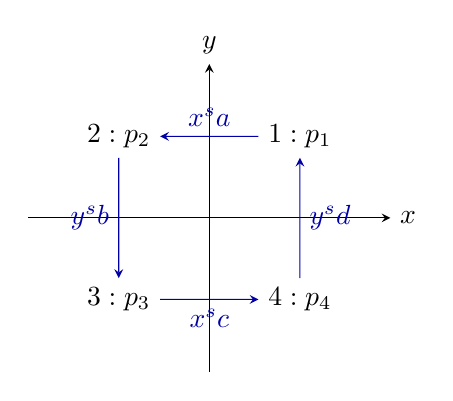
\begin{tikzpicture}[scale=1.15,>=stealth]
\draw[->] (-2,0)--(2,0) node[right] {\(x\)};
\draw[->] (0,-1.7)--(0,1.7) node[above] {\(y\)};
\node (q1) at (1,0.9) {\(1:p_1\)};
\node (q2) at (-1,0.9) {\(2:p_2\)};
\node (q3) at (-1,-0.9) {\(3:p_3\)};
\node (q4) at (1,-0.9) {\(4:p_4\)};
\draw[->,blue!65!black] (q1)--(q2) node[midway,above] {\(x^sa\)};
\draw[->,blue!65!black] (q2)--(q3) node[midway,left] {\(y^sb\)};
\draw[->,blue!65!black] (q3)--(q4) node[midway,below] {\(x^sc\)};
\draw[->,blue!65!black] (q4)--(q1) node[midway,right] {\(y^sd\)};
\end{tikzpicture}
\end{center}
相加得到环行相容条件
\[
x^s(a+c)+y^s(b+d)=0.
\]
这一条件也充分：给定 \(p_1,a,b,c,d\) 后，沿前三条边依次定义 \(p_2,p_3,p_4\)，相容等式恰好保证最后一条边的等式成立。因此没有遗漏其他环行条件。又因 \(x^s,y^s\) 互素，全部关系为
\[
a+c=y^s h,\qquad b+d=-x^s h\qquad(h\in S).
\]
证明也很直接：\(x^s\mid y^s(b+d)\) 推出 \(x^s\mid b+d\)，写 \(b+d=-x^sh\) 后再约去 \(x^s\)。这正是两生成元 \((x^s,y^s)\) 的合冲计算。

\ProseParagraphBreak
取 \(p=p_1\)，依次回代得到全部解
\[
\begin{aligned}
(p_1,p_2,p_3,p_4)
={}&p(1,1,1,1)+a(0,x^s,x^s,0)\\
&+b(0,0,y^s,y^s)+h(0,0,0,x^sy^s).
\end{aligned}
\]
这四个向量的系数唯一：先读第一坐标求 \(p\)，再由第二、第三、第四坐标顺次求 \(a,b,h\)。所以边条件解模是自由分次模
\[
S\oplus S(-s)^2\oplus S(-2s).
\]
四个自由生成元的内次数分别为 \(0,s,s,2s\)，所以这也是前面次数平移自由模的具体应用。其非零区域可以直接对照下面的图；灰色表示该生成元可能非零的象限，坐标轴上的值由相邻多项式一致决定。
\begin{center}
\begin{tikzpicture}[scale=0.75]
\begin{scope}[shift={(0,0)}]
\fill[gray!25] (-1,-1) rectangle (1,1);
\draw (-1.2,0)--(1.2,0);\draw (0,-1.2)--(0,1.2);
\node[below] at (0,-1.3) {\((1,1,1,1)\)};
\end{scope}
\begin{scope}[shift={(3.5,0)}]
\fill[gray!25] (-1,-1) rectangle (0,1);
\draw (-1.2,0)--(1.2,0);\draw (0,-1.2)--(0,1.2);
\node[below] at (0,-1.3) {左半平面：\(x^s\)};
\end{scope}
\begin{scope}[shift={(7,0)}]
\fill[gray!25] (-1,-1) rectangle (1,0);
\draw (-1.2,0)--(1.2,0);\draw (0,-1.2)--(0,1.2);
\node[below] at (0,-1.3) {下半平面：\(y^s\)};
\end{scope}
\begin{scope}[shift={(10.5,0)}]
\fill[gray!25] (0,-1) rectangle (1,0);
\draw (-1.2,0)--(1.2,0);\draw (0,-1.2)--(0,1.2);
\node[below] at (0,-1.3) {右下：\(x^sy^s\)};
\end{scope}
\end{tikzpicture}
\end{center}
前三个生成元只改变全平面或一侧半平面；第四个在右下象限同时含两个边界方程的幂，因而可以只修正这个角部，又不破坏两条邻边上的 \(C^r\) 条件。其系数 \(h\) 不由前三片决定，正是独立的角部修正。

\ProseParagraphBreak
四个生成元确实在原点也是 \(C^r\) 的。第二个对应左半平面上的 \(x^s\)、右半平面上的零，第三个对应下半平面上的 \(y^s\)、上半平面上的零；第四个是右半平面取 \(x^s\)、左半平面取零的函数，与下半平面取 \(y^s\)、上半平面取零的函数的乘积。每个一元分片函数的前 \(r=s-1\) 阶导数都在零处连续，乘以全局多项式及有限相加保持 \(C^r\)。因此上述全部解恰为整个平面的样条，顶点处没有遗漏的条件。

\ProseParagraphBreak
记 \(N(j)=\binom{j+2}{2}\) 当 \(j\ge0\)，而 \(N(j)=0\) 当 \(j<0\)。它是二元全次数不超过 \(j\) 的多项式空间维数。上述唯一表示逐项保持次数，故
\[
\dim_{\mathbb R}C_d^r(\Delta)=N(d)+2N(d-s)+N(d-2s).
\]
例如连续分片二次多项式对应 \(r=0,d=2\)，维数为 \(6+2\cdot3+1=13\)；若要求一阶光滑，则 \(r=1\)，维数变为 \(6+2=8\)。环行条件中的辅助元 \(h\) 正是四条边约束之间的关系所留下的自由量。这说明为什么实际维数不能只用四片的系数总数减去表面上列出的方程数。


\begin{chaptersummary}
自由消解逐层记录生成元之间的关系。分次极小性使微分在剩余域上变为零，因而各层各次的自由秩恰为 Tor 的分次维数。Hilbert 合冲定理进一步说明，在 \(n\) 个变量的多项式环上，有限生成分次模的极小自由消解不会超过 \(n\) 层。

\ProseParagraphBreak
计算时，模项序与 Schreyer 构造给出全部核关系，单位微分项则指出可以删去的可缩部分。正确的记录既要有微分相乘为零的等式，也要有像等于核的依据。Hilbert 级数能由各层次数的交错和恢复，但无法反过来决定 Betti 表；初始理想的单项式计数也必须与原理想的消解信息分开。样条实例把光滑拼接化为整除关系，进一步说明核、合冲模和次数计数怎样共同回答一个具体问题。
\end{chaptersummary}

\BookExercises
除题目另作说明外，多项式环均取标准分次。

\begin{exercise}\label{b3:ex:21-common-factor}
设 \(k\) 为域，在 \(S=k[x,y]\) 中令 \(I=(x^2,xy^2)\)。求 \(I\) 的全部关系，写出 \(S/I\) 的极小自由消解、分次 Betti 数与 Hilbert 级数。
\end{exercise}
\begin{solution}
若 \(ax^2+bxy^2=0\)，约去 \(x\) 得 \(ax+by^2=0\)。因 \(x,y\) 互素，\(b=-cx\)、\(a=cy^2\)。故消解为
\[
0\rightarrow S(-4)\xrightarrow{\binom{y^2}{-x}}S(-2)\oplus S(-3)
\xrightarrow{(x^2\ xy^2)}S\rightarrow S/I\rightarrow0.
\]
左映射单射，其余正合性由上述全部关系计算得出；各微分项在 \((x,y)\) 中，故极小。非零 Betti 数为 \(\beta_{0,0}=\beta_{1,2}=\beta_{1,3}=\beta_{2,4}=1\)，级数为 \((1-t^2-t^3+t^4)/(1-t)^2\)。标准单项式 \(y^a\ (a\ge0)\)、\(x\)、\(xy\) 也给出 \(1/(1-t)+t+t^2\)。
\end{solution}

\begin{exercise}\label{b3:ex:21-nakayama-bound}
设 \(k\) 为域，取 \(S=k[x]\)、\(M=k[x,x^{-1}]/k[x]\)，以通常次数分次。写出 \(M\) 的齐次 \(k\) 基，证明 \(M=xM\ne0\) 而 \(M_x=0\)，并说明分次 Nakayama 引理为何不适用。
\end{exercise}
\begin{solution}
齐次基为 \(\overline{x^{-r}}\ (r\ge1)\)，基向量的次数为 \(-r\)，故 \(M\ne0\) 且非零次数没有下界。又 \(\overline{x^{-r}}=x\overline{x^{-(r+1)}}\)，所以 \(M=xM\)。每个元素只涉及有限个负指数，乘足够大的 \(x\) 次幂后就落入 \(k[x]\)，在商中为零；因此局部化 \(M_x\) 为零。有限组生成元有共同最低次数，乘非负次数多项式不能生成更低次数，故 \(M\) 也非有限生成。\Cref{b3:lem:graded-nakayama}所需的次数下界在这里缺失。
\end{solution}

\begin{exercise}\label{b3:ex:21-direct-sum-shifts}
设 \(k\) 为域，\(S=k[x,y]\)，求 \(M=S/(x^2)\oplus (S/(y))(-1)\) 的极小自由消解与分次 Betti 数。
\end{exercise}
\begin{solution}
两部分分别由乘 \(x^2\) 与乘 \(y\) 的单射消解，直和后为
\[
0\rightarrow S(-2)^2\xrightarrow{\left(\begin{smallmatrix}x^2&0\\0&y\end{smallmatrix}\right)}
S\oplus S(-1)\rightarrow M\rightarrow0.
\]
第二行目标基次数一，故第二列的 \(y\) 仍使总次数为二。矩阵项都在极大齐次理想中，因此 \(\beta_{0,0}=\beta_{0,1}=1\)、\(\beta_{1,2}=2\)。
\end{solution}

\begin{exercise}\label{b3:ex:21-detect-localization}
设 \(k\) 为域，\(S=k[x_1,\ldots,x_n]\)、\(\mathfrak m=(x_1,\ldots,x_n)\)，\(M\) 为有限生成分次 \(S\) 模。证明 \(M_{\mathfrak m}=0\) 当且仅当 \(M=0\)。进一步说明分次极小消解局部化于 \(\mathfrak m\) 后仍极小。
\end{exercise}
\begin{solution}
若 \(M_{\mathfrak m}=0\)，取有限组生成元并合并各自使其为零的分母，得 \(s\notin\mathfrak m\) 且 \(sM=0\)。写 \(s=c+s_+\)、\(c\in k^\times\)，模 \(\mathfrak m\) 得 \(c(M/\mathfrak mM)=0\)，故商为零，再由\cref{b3:lem:graded-nakayama}得 \(M=0\)。反向直接成立。局部化保持正合与自由，极小微分的系数仍落入 \(\mathfrak mS_{\mathfrak m}\)，所以得到局部极小消解，且非零自由项不会消失。
\end{solution}

\begin{exercise}\label{b3:ex:21-projective-graded-free}
设 \(k\) 为域，\(S=k[x,y]\)，\(F=S(-2)\oplus S\)，记两个齐次基向量为 \(e_1,e_2\)，其内次数分别为二、零。考虑矩阵
\[
E=\begin{pmatrix}1&0\\xy&0\end{pmatrix}.
\]
验证它定义一个保持次数的幂等自同态，求 \(P=\operatorname{im}E\)、\(Q=\ker E\) 的齐次自由基和次数平移，并写出 \(F=P\oplus Q\) 的分次分解。
\end{exercise}
\begin{solution}
有 \(E(e_1)=e_1+xy e_2\)、\(E(e_2)=0\)，两者分别为次数二的齐次向量和零向量，所以 \(E\) 保持次数；直接计算得 \(E^2=E\)。其像以 \(e_1+xy e_2\) 为齐次自由基，次数二，故 \(P\cong S(-2)\)；核以 \(e_2\) 为齐次自由基，次数零，故 \(Q\cong S\)。分解由
\[
a e_1+b e_2=a(e_1+xy e_2)+(b-a xy)e_2
\]
给出，两个分量的交为零。对齐次向量，右边两项仍具有相同的总内次数，所以这是分次直和分解。它具体实现了\cref{b3:prop:graded-projective-free}中的齐次自由性，不能仅按矩阵系数的次数忽略目标基的次数平移。
\end{solution}

\begin{exercise}\label{b3:ex:21-polynomial-sequence-point}
设 \(k\) 为域，把\cref{b3:lem:polynomial-module-sequence}用于 \(A=k\)、\(B=k[t]\)、\(M=k\)，其中 \(t\) 作用为乘 \(\lambda\in k\)。写出对应短正合列，并由它计算 \(\operatorname{Tor}_1^B(M,M)\)。
\end{exercise}
\begin{solution}
两份 \(B\otimes_kM\) 都同构于 \(B\)，\(\delta\) 成为乘 \(t-\lambda\)，而 \(\varepsilon\) 是在 \(\lambda\) 处求值。因此得到 \(0\rightarrow B\xrightarrow{t-\lambda}B\rightarrow M\rightarrow0\)。张量 \(M\) 后微分为零，故 \(\operatorname{Tor}_1^B(M,M)\simeq M\)。当 \(\lambda\ne0\) 时该例按通常分次并非分次模例子，但引理本来适用于任意模。
\end{solution}

\begin{exercise}\label{b3:ex:21-infinite-singular-resolution}
设 \(k\) 为域，\(R=k[\varepsilon]/(\varepsilon^2)\)。证明 \(k=R/(\varepsilon)\) 有无限极小自由消解，计算全部 \(\operatorname{Tor}_i^R(k,k)\)，并指出 Hilbert 合冲定理不能直接用于此环的原因。
\end{exercise}
\begin{solution}
乘 \(\varepsilon\) 的核与像均为 \(k\varepsilon\)，所以
\(\cdots\xrightarrow{\varepsilon}R\xrightarrow{\varepsilon}R\rightarrow k\rightarrow0\)
正合。局部极大理想为 \((\varepsilon)\)，因此消解极小，张量 \(k\) 后全为零微分，得每个 \(i\ge0\) 的 Tor 均为 \(k\)。所以投射维数无限。\(R\) 是多项式环的商而非域上的多项式环；商去非零理想不保持上述整体维数上界。
\end{solution}

\begin{exercise}\label{b3:ex:21-cubic-powers}
设 \(k\) 为域，在 \(S=k[x,y,z]\) 中写出 \(S/(x^2,y^2,z^2)\) 的极小消解各项、分次 Betti 数和 Hilbert 级数，不必把所有微分展开成矩阵。
\end{exercise}
\begin{solution}
逐次商后每个新变量的平方仍是非零因子：商可按其余变量的单项式写成关于该变量的多项式，乘其平方只是平移指数。因此用 Koszul 消解得
\(F_0=S\)、\(F_1=S(-2)^3\)、\(F_2=S(-4)^3\)、\(F_3=S(-6)\)。微分系数为变量平方，故极小，\(\beta_{i,2i}=\binom3i\)。级数为 \((1-t^2)^3/(1-t)^3=(1+t)^3\)，总维数八，也由各变量指数为零或一的八个单项式得到。
\end{solution}

\begin{exercise}\label{b3:ex:21-cancel-hilbert-not-exact}
设 \(k\) 为域，\(S=k[x]\) 取标准分次，\(M=S/(x)\)。考虑保持次数的增广列
\[
0\longrightarrow S(-1)\oplus S\xrightarrow{\mathrm{d}}S^2
\xrightarrow{\varepsilon}M\longrightarrow0,
\]
其中 \(\mathrm{d}(a,b)=(xa,0)\)、\(\varepsilon(c,d)=c\bmod x\)。验证 \(\varepsilon\mathrm{d}=0\)，比较自由项的 Hilbert 交错和与 \(H_M(t)\)，并计算 \(\ker\mathrm{d}\) 及 \(\ker\varepsilon/\operatorname{im}\mathrm{d}\)，判断它是否为 \(M\) 的自由消解。
\end{exercise}
\begin{solution}
由 \(xa\bmod x=0\)，有 \(\varepsilon\mathrm{d}=0\)，且 \(\varepsilon\) 满射。自由项的交错和为
\[
\frac{2}{1-t}-\frac{t+1}{1-t}=1=H_M(t).
\]
然而，整环性给出 \(\ker\mathrm{d}=0\oplus S\cong S\)。又
\(\ker\varepsilon=xS\oplus S\)、\(\operatorname{im}\mathrm{d}=xS\oplus0\)，所以 \(\ker\varepsilon/\operatorname{im}\mathrm{d}\cong S\)。两处都不正合，故这不是消解。两个多出的非零模具有相同 Hilbert 级数，恰好在交错和中抵消；与\cref{b3:exm:hilbert-euler-not-exact}一样，Euler 计数不能代替核与像的检验。
\end{solution}

\begin{exercise}\label{b3:ex:21-rank-euler}
设 \(k\) 为域，\(n\ge1\)，\(S=k[x_1,\ldots,x_n]\) 取标准分次，\(M\ne0\) 为有限生成分次挠 \(S\) 模。记 \(B(M)=\sum_{i=0}^n\beta_i(M)\)。证明 \(B(M)\ge2\)，且等号成立当且仅当存在整数 \(a\) 和非零的正次数齐次多项式 \(f\in S\)，使 \(M\cong(S/(f))(-a)\)。
\end{exercise}
\begin{solution}
置 \(\mathfrak m=(x_1,\ldots,x_n)\)。Hilbert 合冲定理使极小消解在第 \(n\) 层以后为零，所以 \(B(M)\) 是全部 Betti 数的有限总和。\(M\ne0\) 给出 \(\beta_0\ge1\)。若 \(\beta_1=0\)，则 \(F_1=0\)，正合性使 \(F_0\cong M\)，与非零自由模不能为挠模矛盾；因此 \(\beta_1\ge1\)，遂有 \(B(M)\ge2\)。

若等号成立，则 \(\beta_0=\beta_1=1\)，其余 Betti 数全为零。极小消解因此为
\[
0\longrightarrow S(-b)\xrightarrow{f}S(-a)
\longrightarrow M\longrightarrow0.
\]
左映射单射使 \(f\ne0\)，保持次数使 \(f\) 齐次且次数为 \(b-a\)，极小性又使 \(f\in\mathfrak m\)，故 \(b-a>0\)。余核就是 \((S/(f))(-a)\)。反之，对这样的 \(f\)，乘 \(f\) 在整环上单射，所给两项消解极小，所以总 Betti 数为二。这个结论也符合\cref{b3:prop:betti-rank-euler}中的 \(\beta_0-\beta_1=0\)。
\end{solution}

\begin{exercise}\label{b3:ex:21-mixed-shifts}
设 \(k\) 为域，在 \(S=k[x,y]\) 中考虑行矩阵 \((x^2\ y)\)。确定使其保持次数的自由项，求其核以及余核 \(S/(x^2,y)\) 的极小消解，并检验每个矩阵项的次数。
\end{exercise}
\begin{solution}
源为 \(S(-2)\oplus S(-1)\)，目标为 \(S\)。由互素性，全部关系由 \((-y,x^2)\) 生成，其总次数是三，所以左项为 \(S(-3)\)。第一列系数 \(-y\) 的次数为 \(3-2=1\)，第二列系数 \(x^2\) 的次数为 \(3-1=2\)。得到 \(S/(x^2,y)\) 的长度二极小消解，首映射因整环性单射。
\end{solution}

\begin{exercise}\label{b3:ex:21-different-components}
设 \(k\) 为域，\(F=k[x,y]e_1\oplus k[x,y]e_2\)，取位置优先且 \(e_1\succ e_2\) 的模项序。证明 \(g_1=xe_1+e_2\)、\(g_2=ye_2\) 是其生成子模的 Gröbner 基，并求全部合冲关系。
\end{exercise}
\begin{solution}
两首项位置不同，不存在需检验的 \(S\)-向量，故由\cref{b3:prop:module-groebner-algorithm}为 Gröbner 基。也可直接看：若 \(a\ne0\)，\(ag_1+bg_2\) 的第一分量为 \(ax\ne0\)，首项被 \(xe_1\) 整除；若 \(a=0\)，非零首项被 \(ye_2\) 整除。若总和为零，第一分量给出 \(a=0\)，第二分量再得 \(b=0\)，所以合冲模为零。
\end{solution}

\begin{exercise}\label{b3:ex:21-same-component}
设 \(k\) 为域，\(F=k[x,y]e_1\oplus k[x,y]e_2\)，\(G=(x^2e_1,ye_1,e_2)\)。计算其 Schreyer 关系，并求 \(F/(G)\)。
\end{exercise}
\begin{solution}
只有前两个首项位置相同，得到关系 \(y\epsilon_1-x^2\epsilon_2\)。第三位置无法与其余项抵消，所以它生成全部合冲模。商中 \(e_2=0\)，第一分量模掉 \((x^2,y)\)，故 \(F/(G)\simeq k[x]/(x^2)\)。要讨论分次消解，可给三个源生成元分别赋次数二、一、零，关系次数为三。
\end{solution}

\begin{exercise}\label{b3:ex:21-redundant-original-generators}
设 \(k\) 为域，\(S=k[x,y,z]\)，令 \(F=(x\ y\ z\ x+y+z)\)、\(G=(x\ y\ z)\)。取
\[
U=\begin{pmatrix}1&0&0\\0&1&0\\0&0&1\\0&0&0\end{pmatrix},
\qquad
V=\begin{pmatrix}1&0&0&1\\0&1&0&1\\0&0&1&1\end{pmatrix}.
\]
先求一个列生成 \(\ker G\) 的矩阵 \(T\)，再利用 \(UT\) 与 \(I_4-UV\) 构造 \(\ker F\) 的全部生成元，写出这些生成元之间的关系，并指出常数关系怎样使消解极小化为变量 \(x,y,z\) 的 Koszul 消解。
\end{exercise}
\begin{solution}
有 \(G=FU\)、\(F=GV\)。变量 \(x,y,z\) 构成正则序列，所以 \(G\) 的核由三列 Koszul 关系生成，记其矩阵为 \(T\)。\Cref{b3:prop:kernel-generator-change}给出 \(\ker F\) 的生成元
\[
\begin{gathered}
s_{12}=(-y,x,0,0),\qquad s_{13}=(-z,0,x,0),\\
s_{23}=(0,-z,y,0),\qquad c=(-1,-1,-1,1).
\end{gathered}
\]
前三列来自 \(UT\)，最后一列是 \(I_4-UV\) 的唯一非零列。若它们的线性组合为零，第四坐标先使 \(c\) 的系数为零；剩下前三列的全部关系由 Koszul 复形的下一层给出，即
\[
z s_{12}-y s_{13}+x s_{23}=0.
\]
关系 \(c\) 表示第四生成元等于前三个之和，其非零常数系数消去一个同为次数一的源、目标基向量。留下的理想生成组为 \((x,y,z)\)，再接上 \(S\to S/(x,y,z)\)，便得到长度三的极小 Koszul 消解。若以理想 \((x,y,z)\) 为末项，则相应消解长二。
\end{solution}

\begin{exercise}\label{b3:ex:21-divisibility-relations}
设 \(k\) 为域，给 \(S=k[x,y]\) 中的三个单项式 \(x^3,x^2y,xy^2\) 求最小关系生成组，并求商环 \(S/(x^3,x^2y,xy^2)\) 的 Hilbert 级数。
\end{exercise}
\begin{solution}
三个生成元都含公共因子 \(x\)，在整环中约去它，关系与 \(x^2,xy,y^2\) 相同，故由 \((y,-x,0)\)、\((0,y,-x)\) 自由生成。所得极小消解各项为 \(S\)、\(S(-3)^3\)、\(S(-4)^2\)，级数为 \((1-3t^3+2t^4)/(1-t)^2\)。约去公共因子不改变关系系数，却改变生成元和关系的内次数。
\end{solution}

\begin{exercise}\label{b3:ex:21-unit-homotopy}
设 \(k\) 为域，\(S=k[x_1,\ldots,x_n]\) 取标准分次，\(a\in\mathbb Z\)、\(c\in k^\times\)。对两项复形 \(0\rightarrow S(-a)\xrightarrow{c}S(-a)\rightarrow0\)，写出恒等映射与零映射之间的链同伦。解释为什么它可以从消解中删去。
\end{exercise}
\begin{solution}
令从低次项到高次项的同伦映射为乘 \(c^{-1}\)，其余同伦分量为零。则两项上分别有 \(\mathrm{d}h=1\)、\(h\mathrm{d}=1\)，故 \(\mathrm{d}h+h\mathrm{d}\) 为恒等。这个复形可缩，特别正合；若它是某消解的直和项，去掉后各同调不变。仅在微分矩阵里看见一个非零常数还须先作相容换基，才能保证它确实构成直和项。
\end{solution}

\begin{exercise}\label{b3:ex:21-tor-socle}
设 \(k\) 为域，\(A=k[x,y]/(x^2,y^3)\)。直接用以 \(A\) 为系数的两元 Koszul 复形求 \(\operatorname{Tor}_2^{k[x,y]}(A,k)\) 的维数与内次数。
\end{exercise}
\begin{solution}
最高同调对应被 \(x,y\) 同时零化的元素。把元素按基 \(1,x,y,xy,y^2,xy^2\) 展开，乘 \(x\) 为零使只剩 \(x,xy,xy^2\) 的组合，再乘 \(y\) 为零只剩 \(kxy^2\)。此元素内次数三，加上 \(e_x\wedge e_y\) 的次数二，所得 Tor 为一维且内次数五，符合完整消解左项 \(S(-5)\)。
\end{solution}

\begin{exercise}\label{b3:ex:21-betti-specialization}
设 \(k\) 为域，\(a\in k\)，在 \(S=k[x,y]\) 中令 \(I_a=(x^2,xy+ay^2,y^3)\)。证明所有 \(S/I_a\) 的 Hilbert 级数相同，但 \(a=0\) 与 \(a\ne0\) 的 Betti 表不同。
\end{exercise}
\begin{solution}
字典序 \(x\succ y\) 下这三个多项式构成 Gröbner 基：前两者的 \(S\)-多项式先约化成 \(a^2y^3\)，第二、第三对约化为 \(ay^4\)，均由 \(y^3\) 消去；第一、第三对首项互素。标准单项式恒为 \(1,x,y,y^2\)，级数为 \(1+2t+t^2\)。

若 \(a\ne0\)，恒等式
\(yx^2-(x-ay)(xy+ay^2)=a^2y^3\)
使第三生成元冗余；前两者互素，构成二次正则序列，非零 Betti 多项式为 \(1,2t^2,t^4\)。若 \(a=0\)，则为正文的 \((x^2,xy,y^3)\)，Betti 多项式为 \(1,2t^2+t^3,t^3+t^4\)。消去三次生成元的系数涉及 \(a^{-2}\)，因此不能把一般参数下的极小化直接代入 \(a=0\)。
\end{solution}

\begin{exercise}\label{b3:ex:21-kernel-certificate}
设 \(k\) 为域，\(S=k[x,y,z]\)、\(F=(x^2\ xy\ xz)\)。有人以
\[
K=\begin{pmatrix}-y&-z\\x&0\\0&x\end{pmatrix}
\]
作为 \(\ker F\) 的生成矩阵。验证 \(FK=0\)，证明它遗漏了关系 \((0,-z,y)\)，补全核的生成组，并写出这些生成元的全部关系。
\end{exercise}
\begin{solution}
直接相乘得 \(FK=0\)，且 \(s_{23}=(0,-z,y)\) 也被 \(F\) 零化。但 \(K\) 的像中每个向量的第二、第三坐标都可被 \(x\) 整除；\(s_{23}\) 的这两坐标不能如此，故它不属于 \(\operatorname{im}K\)。等价地，模掉 \(x\) 后，\(K\) 的像只可能有第一坐标，而 \(s_{23}\) 的后两坐标非零。

在整环中约去 \(F=x(x\ y\ z)\) 的公共因子 \(x\)，得到 \(\ker F=\ker(x\ y\ z)\)。变量 Koszul 复形遂给出全部核生成元
\(s_{12}=(-y,x,0)\)、\(s_{13}=(-z,0,x)\)、\(s_{23}=(0,-z,y)\)，而它们的关系模由 \((z,-y,x)\) 生成，即 \(z s_{12}-y s_{13}+x s_{23}=0\)。所以微分相乘为零只证明给出的列是关系，不能证明全部关系已经找齐。
\end{solution}

\begin{exercise}\label{b3:ex:21-top-degree-bound}
设 \(k\) 为域，\(S=k[x_1,\ldots,x_n]\) 取标准分次，\(M\ne0\) 为有限生成分次 \(S\) 模，\(b\in\mathbb Z\)。若 \(M_j=0\) 对所有 \(j>b\) 成立，证明 \(\beta_{i,j}(M)=0\) 当 \(j>b+i\)。
\end{exercise}
\begin{solution}
以 \(M\) 为系数的变量 Koszul 复形第 \(i\) 项是 \(M(-i)^{\binom ni}\)，其次数 \(j\) 部分为若干 \(M_{j-i}\) 的直和。当 \(j>b+i\) 时该项为零，同调对应次数也为零；再由 Tor 与 Betti 数的等式得到结论。该上界来自各项本身为零，不需要预先求出微分的秩。
\end{solution}


\begin{exercise}\label{b3:ex:21-polynomial-inhomogeneous}
设 \(k\) 为域，在 \(S=k[x,y]\) 上求 \(x^2u+xyv=x^3\) 的全部多项式解，并说明把右端改为 \(x\) 时为何无解。
\end{exercise}
\begin{solution}
整环中约去 \(x\)，得到 \(xu+yv=x^2\)。特解为 \((x,0)\)，核由 \((y,-x)\) 生成，故全部解为 \(u=x+yh,v=-xh\)，\(h\in S\)。右端为 \(x\) 时约去 \(x\) 得 \(xu+yv=1\)，在原点求值即矛盾。若工作环改为 \(S_x\)，则 \((u,v)=(x^{-1},0)\) 是后一方程的解；这再次说明解集依赖工作环。
\end{solution}

\begin{optionalexercise}\label{b3:ex:21-spline-strips}
用直线 \(x=0\) 与 \(x=1\) 将 \(\mathbb R^2\) 分成三条闭区域，每片取 \(\mathbb R[x,y]\) 中的多项式，要求它们作 \(C^r\) 拼接，\(r\ge0\)。求全部解的唯一参数表示，以及每片全次数不超过整数 \(d\ge0\) 时的实向量空间维数。
\end{optionalexercise}
\begin{solution}
置 \(s=r+1\)，按从左到右排列分片。由\cref{b3:prop:spline-divisibility}，全部解唯一写成
\[
(p_1,p_2,p_3)=\bigl(p,\ p+x^sa,\ p+x^sa+(x-1)^sb\bigr),
\qquad p,a,b\in\mathbb R[x,y].
\]
两条直线不相交，因此没有内部顶点的额外拼接问题。若三个分片次数均不超过 \(d\)，由逐次作差可知 \(\deg p\le d\)、\(\deg a,\deg b\le d-s\)；反向这些限制显然足够。于是维数为 \(N(d)+2N(d-s)\)，其中 \(N(j)=\binom{j+2}{2}\) 对 \(j\ge0\)，负指标时为零。这里关系含常数，使用的是次数滤过；不能未经说明就把 \((x-1)^s\) 当成齐次元。
\end{solution}

